\documentclass[11pt]{article}
\usepackage[margin=1in]{geometry}
\usepackage[T1]{fontenc}
\usepackage[utf8]{inputenc}
\usepackage{amsmath, amssymb, amsfonts}
\usepackage{graphicx}
\usepackage{array}
\usepackage{tabularx}
\usepackage{booktabs}
\usepackage{float}
\usepackage{hyperref}
\title{Scientific Analysis of Moral Judgments using Tobit Models with Random Intercepts and Four Empathy Constructs}
\author{Automated Research Pipeline}
\date{abril 11, 2026}
\begin{document}
\maketitle

\section{Dataset and Sample Description}
The empirical foundation of this project rests on two primary experimental datasets: FLORIDA and BUC.  The sample consists of students from both the Floridablanca and Bucaramanga Campuses.  These datasets capture incentivized moral judgments from distinct socio-economic contexts. Participants were presented  with standardized negotiation scenarios where a negotiator's decision resulted in varying degrees of payoff for  themselves, their own group, and a victim group. Under  Option 2: judgment-level relational modeling , each judgment is treated as relational and linked both to a descriptive victim x negotiator scenario shorthand and to hypothesis-specific predictors for N1 (judged negotiator) and N2 (counterpart), observer-side victim alignment when applicable, and additional relational controls.

\section{Primary Estimator in This Run}
The primary inferential branch is the Tobit slot with random intercepts. In practice, each fitted model includes (1 | id), and when id\_case is identifiable as a repeated grouping level the model also includes (1 | id\_case).

\section{Datacard and Variable Definitions}
The following table defines the primary symbols and variables used in the mathematical specifications and hypothesis tests.
\begin{table}[H]
\centering
\caption{Symbols and Variable Dictionary.}
\label{tab:symbols}
\resizebox{\textwidth}{!}{%
\begin{tabular}{ll}
\toprule
Symbol & Definition \\
\midrule
$y_{isjr}$ & Observed moral judgment (Scale: -9 to 9). \\
$y^*_{isjr}$ & Latent moral preference score (unbounded true judgment). \\
$\beta_1$ & The measured effect of a variable on moral judgment (coefficient). \\
$\text{IRI}_i$ & Empathy score: Participant's propensity for empathy across different IRI subscales. \\
$\mathbf{S}_{isj}$ & Relationship structure: The group status of both N1 and N2 negotiators (Ingroup, Outgroup, or Control). \\
$V_{is}$ & Observer-victim match: Whether the observer and victim have matching group affiliations. \\
$G_{isjr}$ & N1 Group Status: The specific group affiliation of the N1 negotiator being judged. \\
$A_{is}$ & Action Taken: Whether the harm was Accepted (A=1) or Rejected (A=0). \\
$C_{isjr}$ & Relational Controls: Other factors that might influence judgment, like age or socioeconomic status. \\
$\text{ICC}$ & Intraclass Correlation: The degree of similarity in judgments within the same participant. \\
\bottomrule
\end{tabular}
}
\end{table}
Option 2: judgment-level relational modeling retains a compact relational shorthand for descriptive summaries, while the executable hypotheses use explicit role-specific N1/N2 predictors and N1\_N2\_same\_faculty as a contextual main effect.

\subsection{Predictor Glossary and Abbreviations}
The regression tables and dynamic figures use compact predictor labels to stay readable. The bullet list below maps those compact labels back to their full meaning and subset-specific interpretation.
\begin{itemize}
  \item \texttt{iri\_fs, iri\_ec, iri\_pt, iri\_pd} [FS, EC, PT, PD]: Active empathy predictors: fantasy, empathic concern, perspective taking, and personal distress. Used in H1/H2/H3 active model.
  \item \texttt{victim\_N1\_groupIn, victim\_N1\_groupOut} [V-N1 In, V-N1 Out]: Victim-to-N1 contrasts relative to the control-labeled baseline. Used in H1/H2/H3 Victim and Bystander.
  \item \texttt{victim\_N2\_groupIn, victim\_N2\_groupOut} [V-N2 In, V-N2 Out]: Victim-to-N2 contrasts relative to the control-labeled baseline. Used in H1/H2/H3 Victim and Bystander.
  \item \texttt{bystander\_N1\_groupIn, bystander\_N1\_groupOut} [B-N1 In, B-N1 Out]: Bystander-to-N1 contrasts relative to the control-labeled baseline. Used in H1/H2/H3 Bystander.
  \item \texttt{bystander\_N2\_groupIn, bystander\_N2\_groupOut} [B-N2 In, B-N2 Out]: Bystander-to-N2 contrasts relative to the control-labeled baseline. Used in H1/H2/H3 Bystander.
  \item \texttt{bystander\_victim\_groupOut} [B-V Out]: Bystander-victim outgroup contrast with bystander-victim ingroup as the reference. Used in H1/H2/H3 Bystander.
  \item \texttt{N1\_N2\_same\_faculty} [SameFac]: Context indicator for whether N1 and N2 belong to the same faculty. Used in H1/H2/H3 Victim and Bystander.
  \item \texttt{victim\_N1\_group*:victim\_N2\_group*} [V-N1 x V-N2]: Victim-side N1-by-N2 interaction block. Used in H2/H3 Victim and Bystander.
  \item \texttt{bystander\_N1\_group*:bystander\_N2\_group*} [B-N1 x B-N2]: Bystander-side N1-by-N2 interaction block. Used in H2/H3 Bystander.
  \item \texttt{bystander\_victim\_group*:bystander\_N1\_group*} [B-V x B-N1]: Bystander-victim by bystander-N1 interaction block. Used in H2/H3 Bystander.
  \item \texttt{bystander\_victim\_group*:bystander\_N2\_group*} [B-V x B-N2]: Bystander-victim by bystander-N2 interaction block. Used in H2/H3 Bystander.
  \item \texttt{iri\_*:victim\_N*\_group*} [FS / EC / PT / PD x V-N...]: Empathy-by-victim-side relational interaction block. Used in H3 Victim.
  \item \texttt{iri\_*:bystander\_N*\_group*} [FS / EC / PT / PD x B-N...]: Empathy-by-bystander-side relational interaction block. Used in H3 Bystander.
  \item \texttt{iri\_*:bystander\_victim\_group*} [FS / EC / PT / PD x B-V]: Empathy-by-bystander-victim interaction block. Used in H3 Bystander.
  \item \texttt{participant\_engineering} [Eng part.]: Participant faculty contrast. Used in H1/H2/H3.
  \item \texttt{sex\_man} [Man]: Sex contrast with woman as the reference. Used in H1/H2/H3.
  \item \texttt{age} [Age]: Participant age in original units. Used in H1/H2/H3.
  \item \texttt{economic\_status} [SES]: Economic status in original units. Used in H1/H2/H3.
\end{itemize}

\subsection{Interpretation of Interaction Terms}
The models herein employ several predefined predictors. It is important to note how interaction terms are interpreted in the context of this behavioral experiment:
\begin{enumerate}
  \item \textbf{Interaction Subsumption:} When an interaction term is statistically significant, it indicates that the effect of one variable depends on the level of the other. Crucially, if the interaction is significant but the constituent main effects are not explicitly significant, their effects are fully subsumed and contextualized by the interaction.
  \item \textbf{Continuous by Discrete Interactions:} For terms like \texttt{iri\_pt:victim\_N1\_groupOut}, a negative coefficient implies that the empathy slope becomes more negative (more severe judgments) under that relational outgroup condition relative to the control-labeled baseline.
  \item \textbf{Discrete by Discrete Interactions:} For terms like \texttt{bystander\_N1\_groupOut:bystander\_N2\_groupOut}, a positive coefficient implies that the joint relational condition is associated with less severe condemnation than expected from the baseline profile.
\end{enumerate}

\section{Hypotheses to Test}
\begin{itemize}
  \item \textbf{H1 (Empathy Effect):} Empathy dimensions are associated with moral judgment severity after conditioning on role-specific N1/N2 relational predictors and the N1-N2 same-faculty context term.
  \item \textbf{H2 (Negotiator-Side Structure):} Moral judgments vary with explicit N1/N2 relational structure and with the participant role. Bystander models retain participant-victim alignment and selective pairwise interactions.
  \item \textbf{H3 (Empathy x Relational Status):} The empathy effect depends on N1/N2 relational status indicators within each role-specific model while retaining relational controls and participant-level random intercepts.
\end{itemize}

\section{Mathematical Approach and Theoretical Foundations}
The analysis employs two complementary estimators for bounded moral judgments. The primary inferential branch is labeled Tobit and estimated with random intercepts, separately by role subset. 
Observed moral judgments ($y_{isjr}$) remain on the original bounded scale from -9 to 9, where lower values indicate harsher condemnation and higher values indicate less severe condemnation. 
The primary model is:

$$y_{isjr} = \beta_0 + \mathbf{x}_{isjr}'\beta + u_i + v_{c(i,s)} + \epsilon_{isjr}$$

where $u_i$ is a participant random intercept and $v_{c(i,s)}$ is an optional case-level random intercept included when the case identifier supports repeated within-case judgments (otherwise the model keeps the participant random intercept only). In implementation terms this corresponds to $(1|id)$ and, when identifiable, $(1|id\_case)$.
Option 2 replaces isolated ingroup/outgroup indicators with explicit judgment-level relational variables built from the paired-group structure of each judgment. The analytic hypothesis models decompose that structure into judged-negotiator status, counterpart-negotiator status, observer-side victim alignment when applicable, and hypothesis-specific interaction blocks.
 H1, H2, and H3 are all estimated separately in the victim and bystander subsets using role-specific relational predictors:

Victim-subset H2:

$$y_{isj,Victim} = \beta_0 + \beta_1 \text{Empathy}_i + \gamma_1 \text{Victim-N1}_{isj} + \gamma_2 \text{Victim-N2}_{isj} + \gamma_3(\text{Victim-N1}_{isj} \times \text{Victim-N2}_{isj}) + \gamma_4\text{SameFac}_{isj} + \boldsymbol{\delta}'\mathbf{Z}_i + u_i + v_{c(i,s)} + \epsilon_{isj}$$

Bystander-subset H2:

$$y_{isj,Obs} = \beta_0 + \beta_1 \text{Empathy}_i + \eta\text{Bystander-Victim}_{isj} + \boldsymbol{\kappa}'(\text{Bystander-Victim}_{isj}\times\text{Bystander-N}_{isj}) + \boldsymbol{\gamma}'\mathbf{R}_{isj} + \gamma_4\text{SameFac}_{isj} + \boldsymbol{\delta}'\mathbf{Z}_i + u_i + v_{c(i,s)} + \epsilon_{isj}$$

H3:

$$y_{isjr} = \beta_0 + \beta_1 \text{Empathy}_i + \boldsymbol{\beta}_2'\mathbf{G}_{isjr} + \boldsymbol{\beta}_3'(\text{Empathy}_i \times \mathbf{G}_{isjr}) + \kappa_1(\text{Bystander-Victim}_{isjr}\times\text{Bystander-N}_{isjr}) + \kappa_2(\text{Empathy}_i\times\text{Bystander-Victim}_{isjr}) + \beta_4\text{SameFac}_{isjr} + \boldsymbol{\delta}'\mathbf{Z}_i + u_i + v_{c(i,s)} + \epsilon_{isjr}$$

For the three-level relational factors (Victim-N1, Victim-N2, Bystander-N1, Bystander-N2), the control-labeled level is the reference category. For bystander-victim alignment, ingroup is the reference category.


\section{Analysis of Sample Size Impact}
The statistical validity of our inferences depends on the trade-off between False Positives (Type I error, $\alpha$) 
and False Negatives (Type II error, $\beta$). Given the clustered nature of our data, sample size impact is not 
merely a count of observations, but a function of cluster correlation.

\subsubsection{Step-by-Step Sensitivity Analysis}
To determine the impact of our sample size on our ability to detect effects, we follow these steps:

1. Calculate the Design Effect (Deff): As multiple judgments are nested within individuals, we adjust for the Intraclass Correlation (ICC).
$$Deff = 1 + (m - 1) \times ICC$$
where $m$ is the average number of scenarios per participant. 

2. Determine the Effective Sample Size (ESS): The ESS represents the number of independent observations that would provide the same statistical power as our clustered sample.
$$ESS = \frac{n_{total}}{Deff}$$

3. Inference Impact: A higher ICC reduces the ESS, thereby increasing standard errors in our Tobit random-intercepts coefficients. 
If the ESS is low, our models become 'conservative', increasing the risk of Type II errors (failing to support a hypothesis). 
By using role-specific Tobit random-intercepts estimation, we ensure that inference acknowledges this reduced information density, protecting the integrity of our Type I error threshold ($\alpha = 0.05$).

Based on the current run, the observed Intraclass Correlation (ICC) is 0.088, with an Effective Sample Size (ESS) of 1819.3.

\section{Descriptive Statistics}
The empathy profile of the sample is visualized in Figure \ref{fig:radar}, showing the average scores across the four IRI subscales (Fantasy, Empathic Concern, Perspective Taking, Personal Distress), each scored 0–4 (scale mean per subscale).
\begin{figure}[H]
\centering
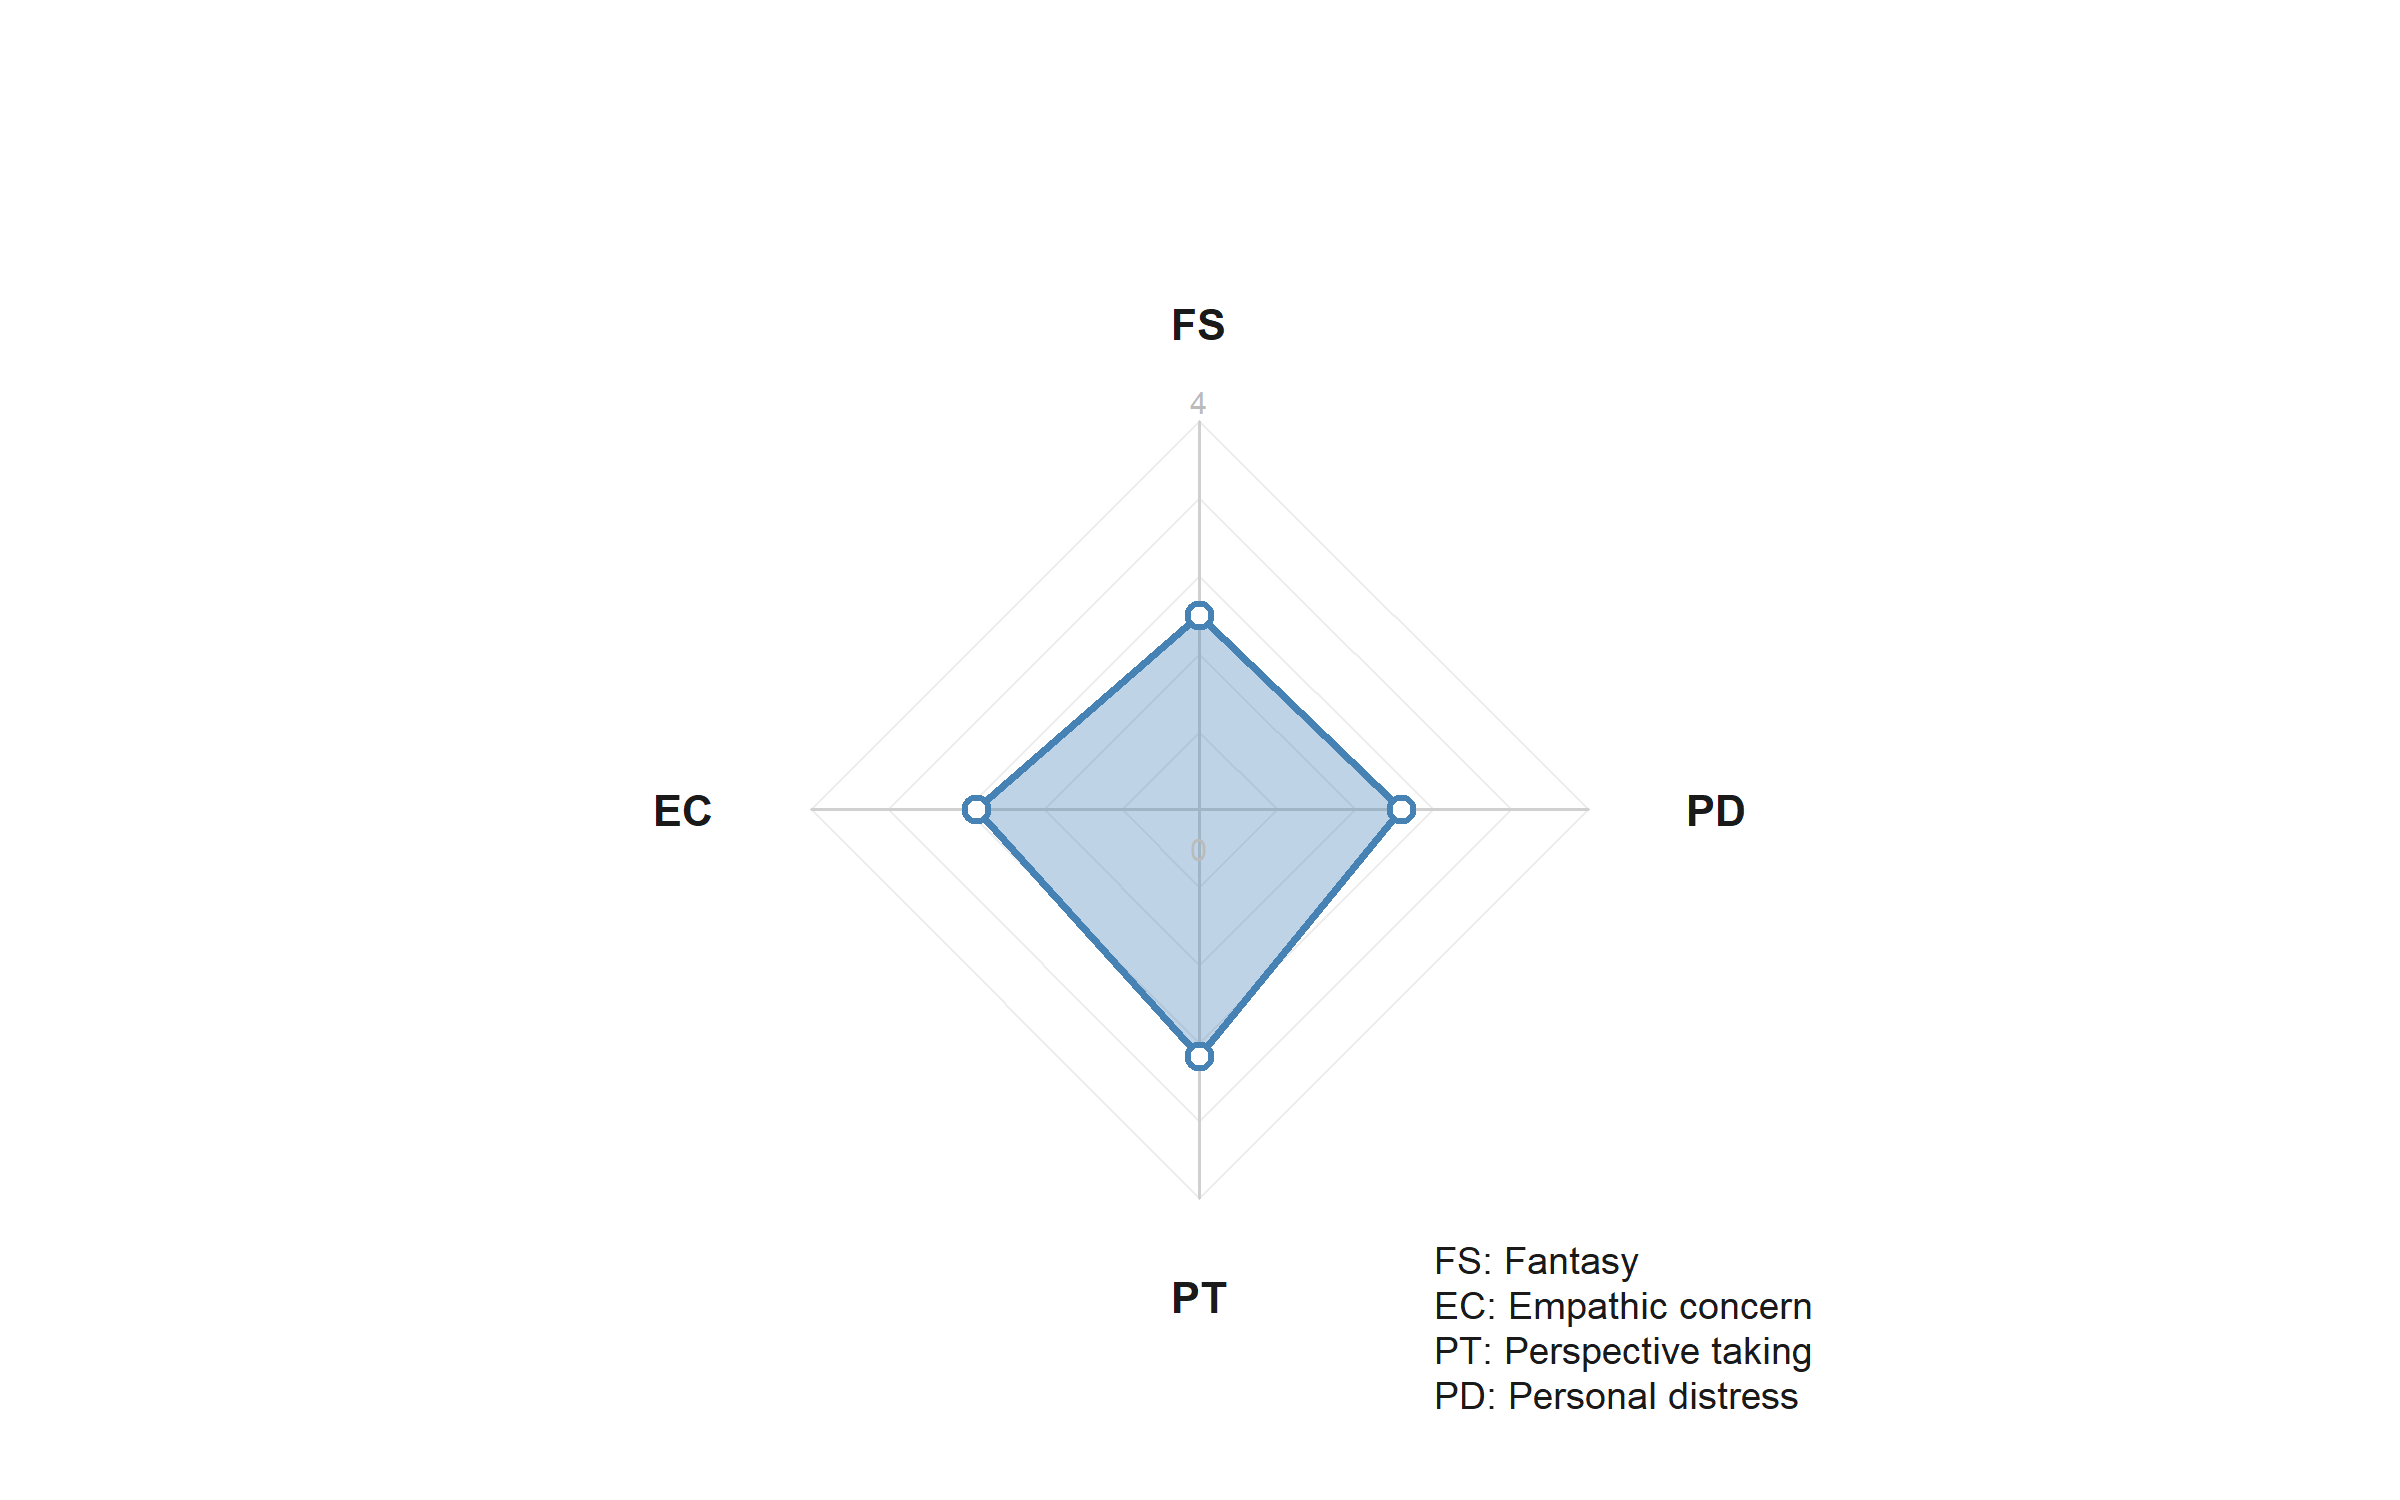
\includegraphics[width=0.92\textwidth]{../figures/figure_03_iri_latent_variable_averages.png}
\caption{IRI subscale averages (radar plot; scale 0--4 per subscale).}
\label{fig:radar}
\end{figure}
Figure \ref{fig:severity_panels} shows severity distributions pooled across the full analytical sample, broken down by N1 group membership (\textit{group\_target}: Ingroup, Outgroup, Control). Figures \ref{fig:victim_case_panels} and \ref{fig:bystander_case_panels} expand the descriptive view to the six explicit victim x negotiator faculty configurations, with separate panel rows for accepted and rejected harmful deals inside each role subset. Figures \ref{fig:accepted_case_panels} and \ref{fig:rejected_case_panels} then pool the full analytical sample and show the accepted- and rejected-decision distributions across those same six case configurations.
\begin{figure}[H]
\centering
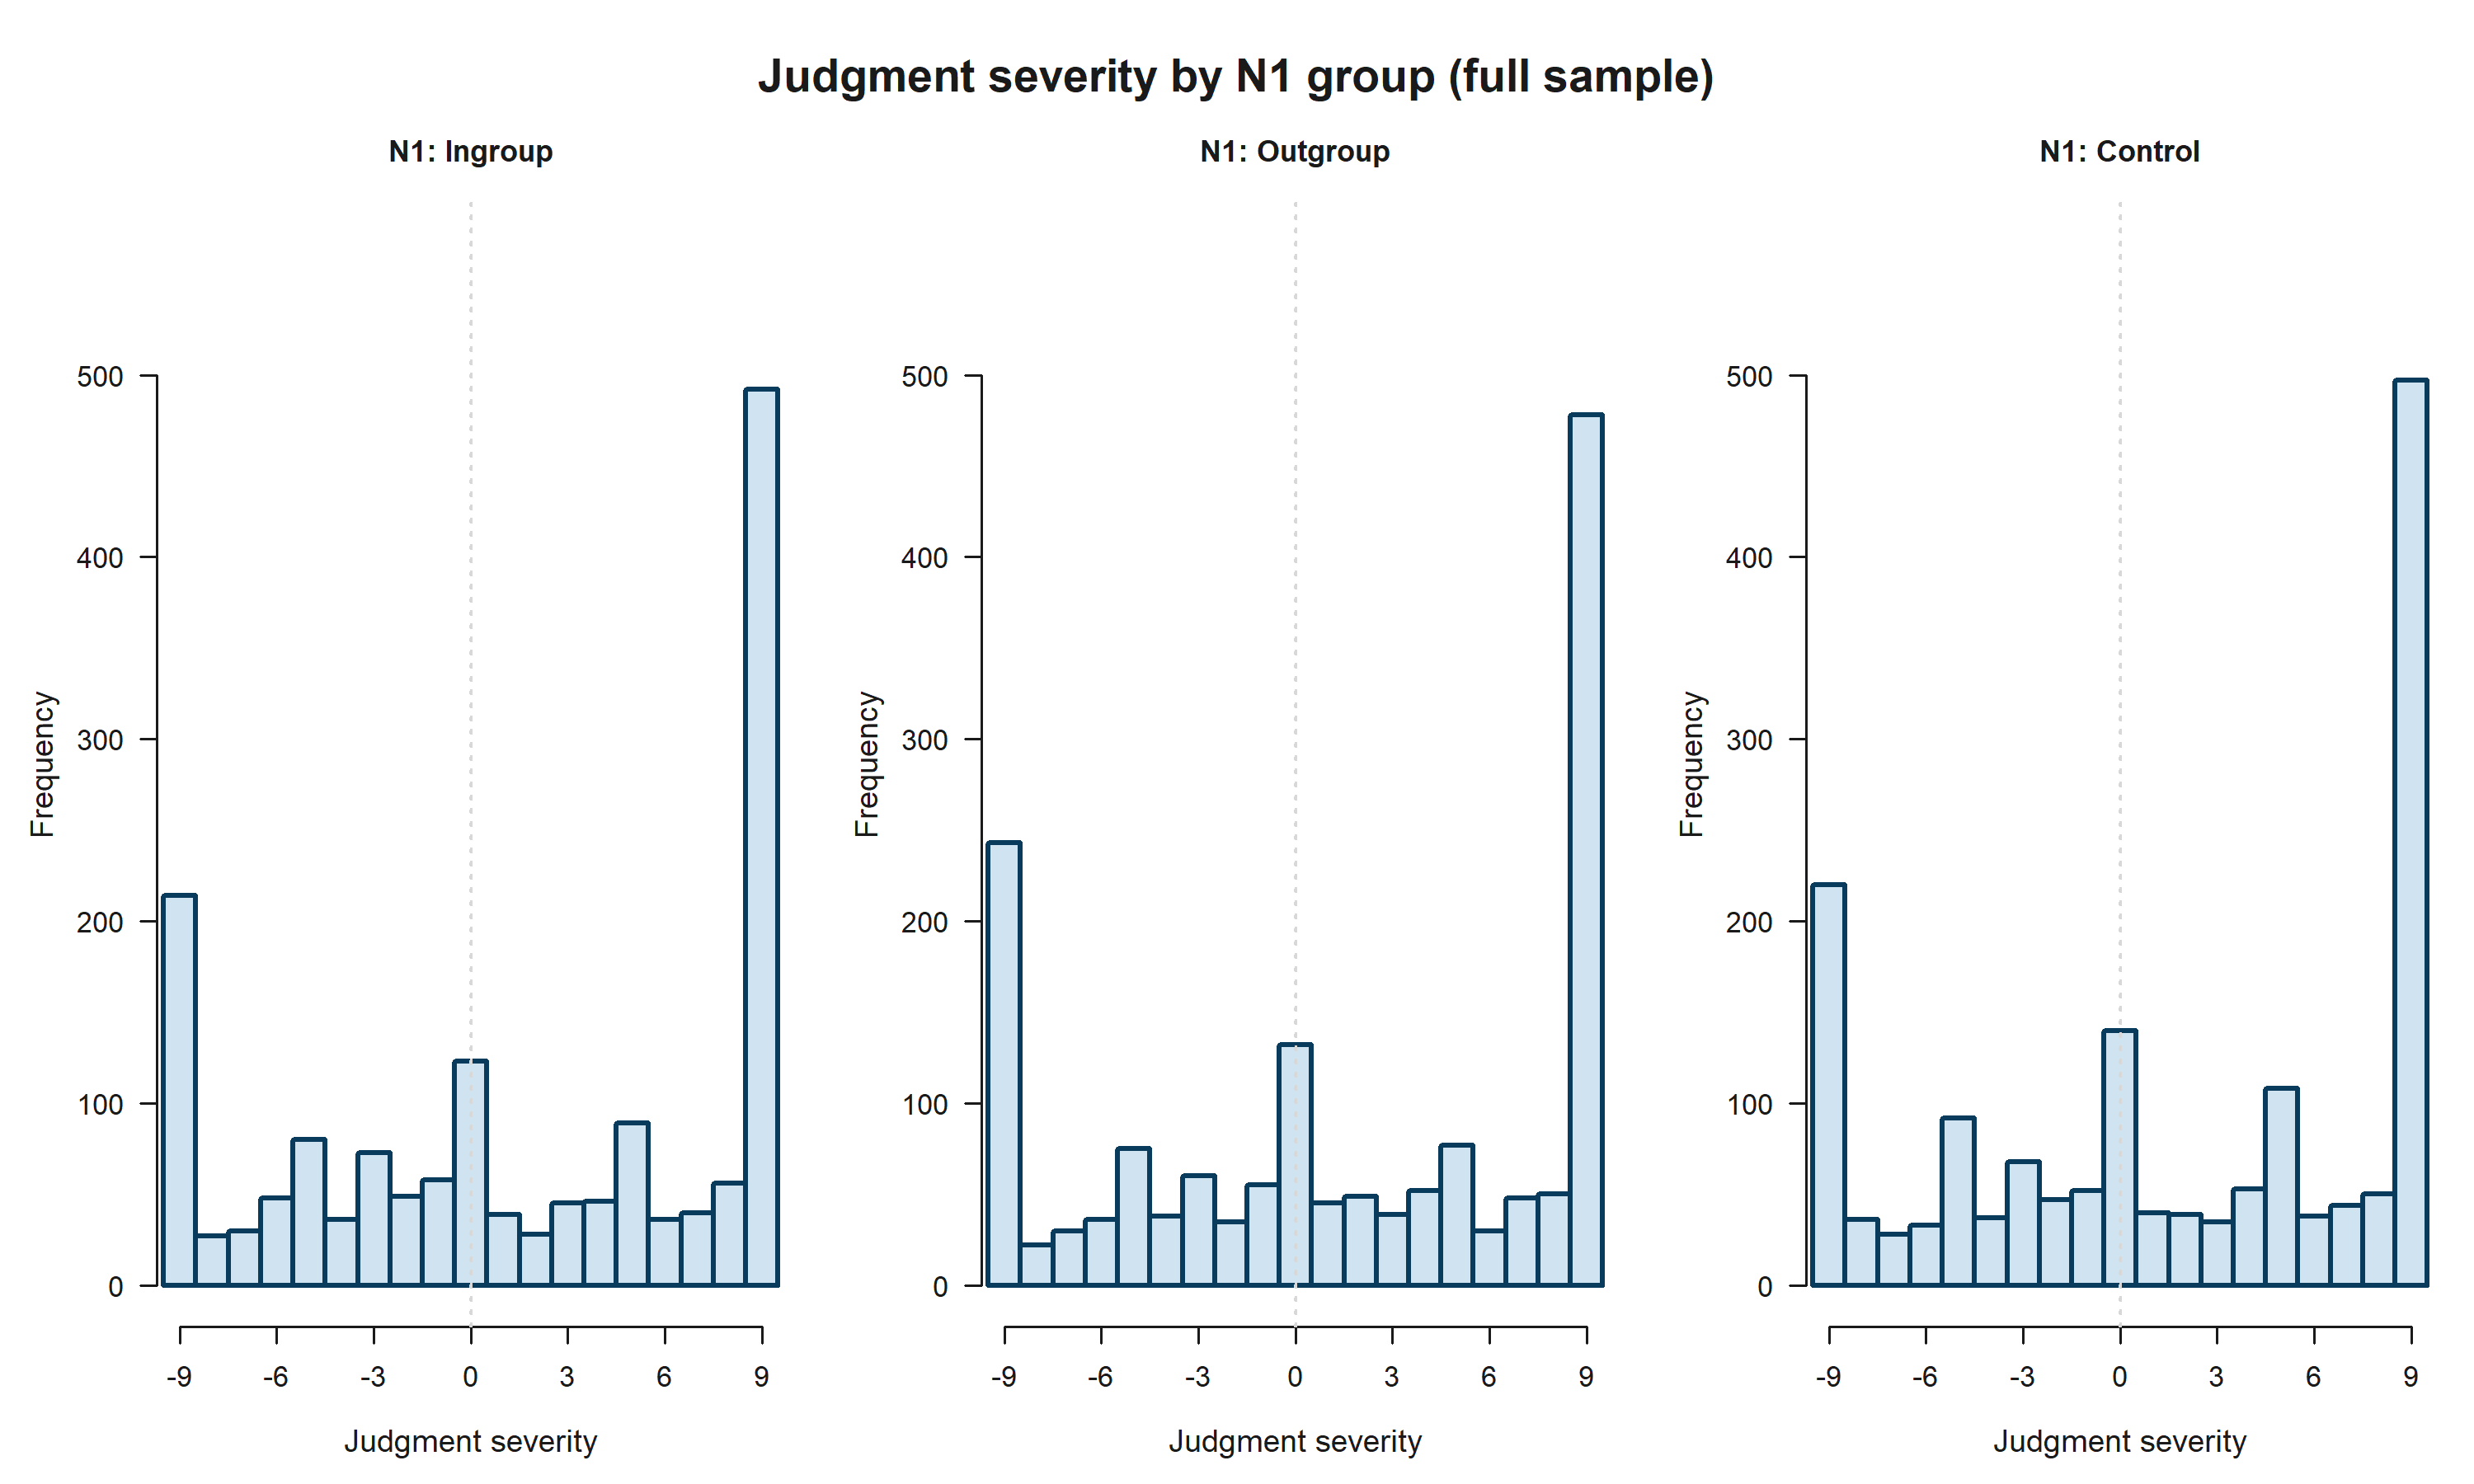
\includegraphics[width=0.92\textwidth]{../figures/figure_04_judgment_distributions_by_n1_status.png}
\caption{Judgment severity by N1 group (\textit{group\_target}: Ingroup, Outgroup, Control) --- full analytical sample, scale $-9$ to $9$.}
\label{fig:severity_panels}
\end{figure}
\begin{figure}[H]
\centering
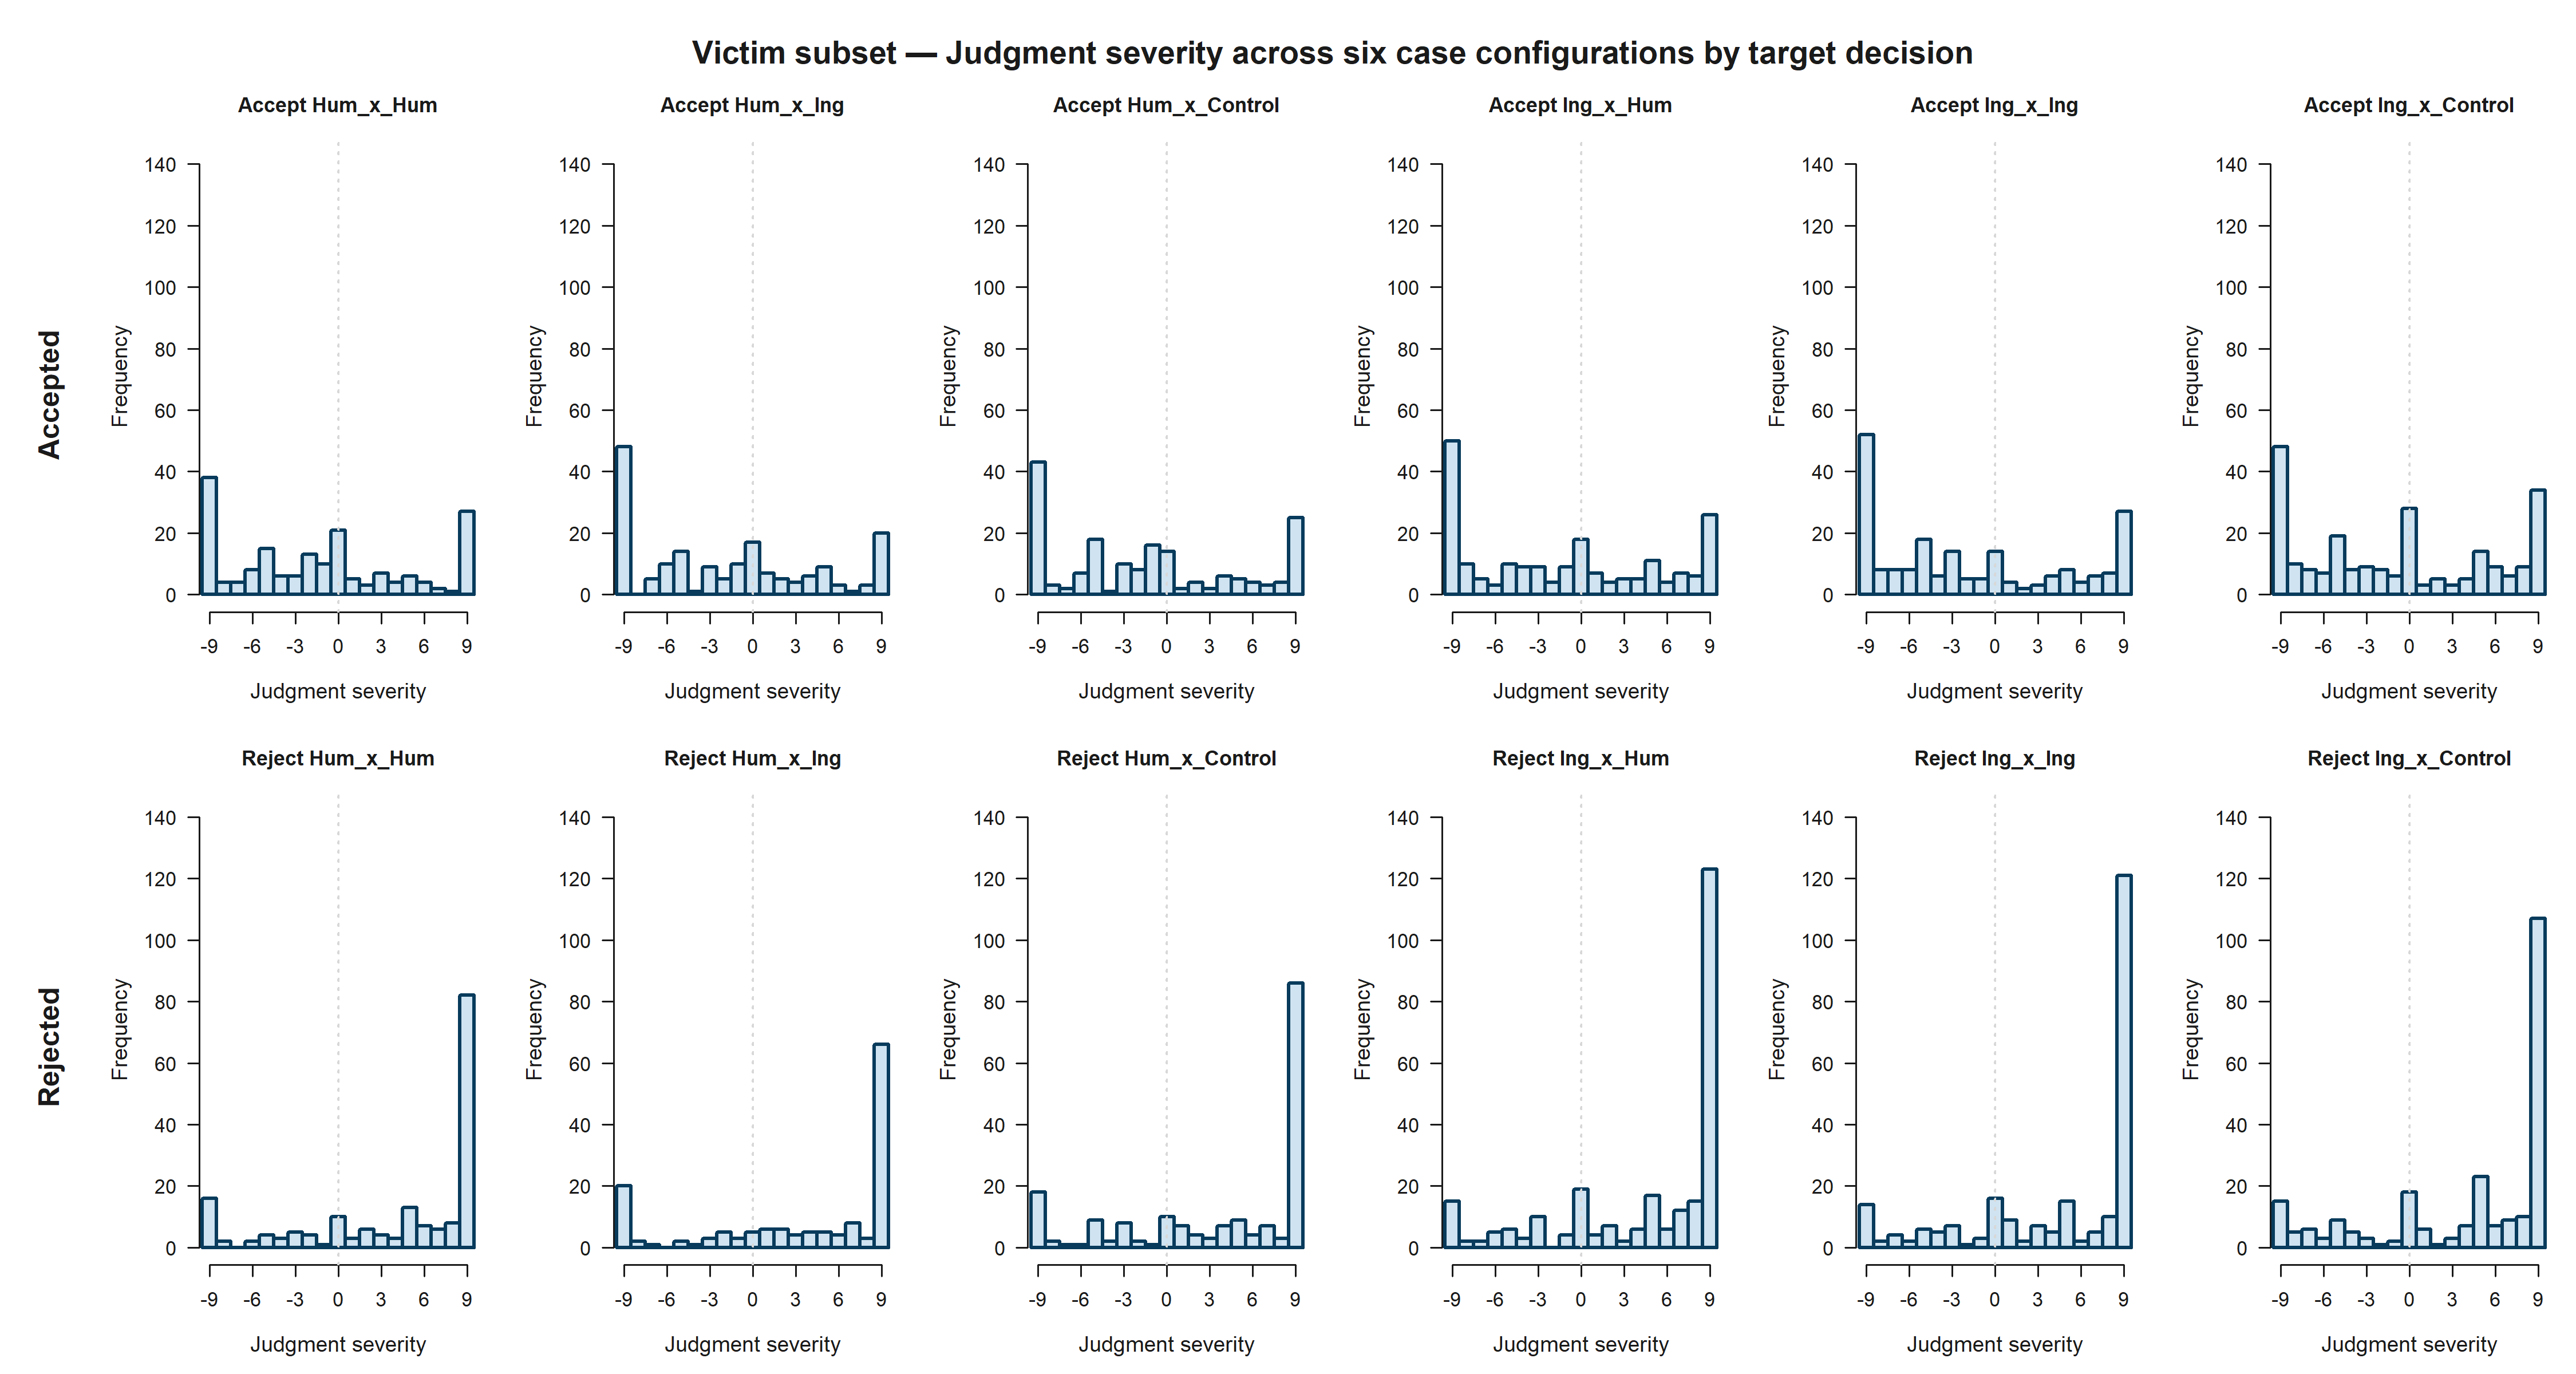
\includegraphics[width=0.92\textwidth]{../figures/figure_06_victim_subset_judgment_distributions_across_six_case_configurations.png}
\caption{Victim-subset judgment distributions across the six explicit victim x negotiator faculty configurations, with separate rows for accepted and rejected harmful deals, scale $-9$ to $9$.}
\label{fig:victim_case_panels}
\end{figure}
\begin{figure}[H]
\centering
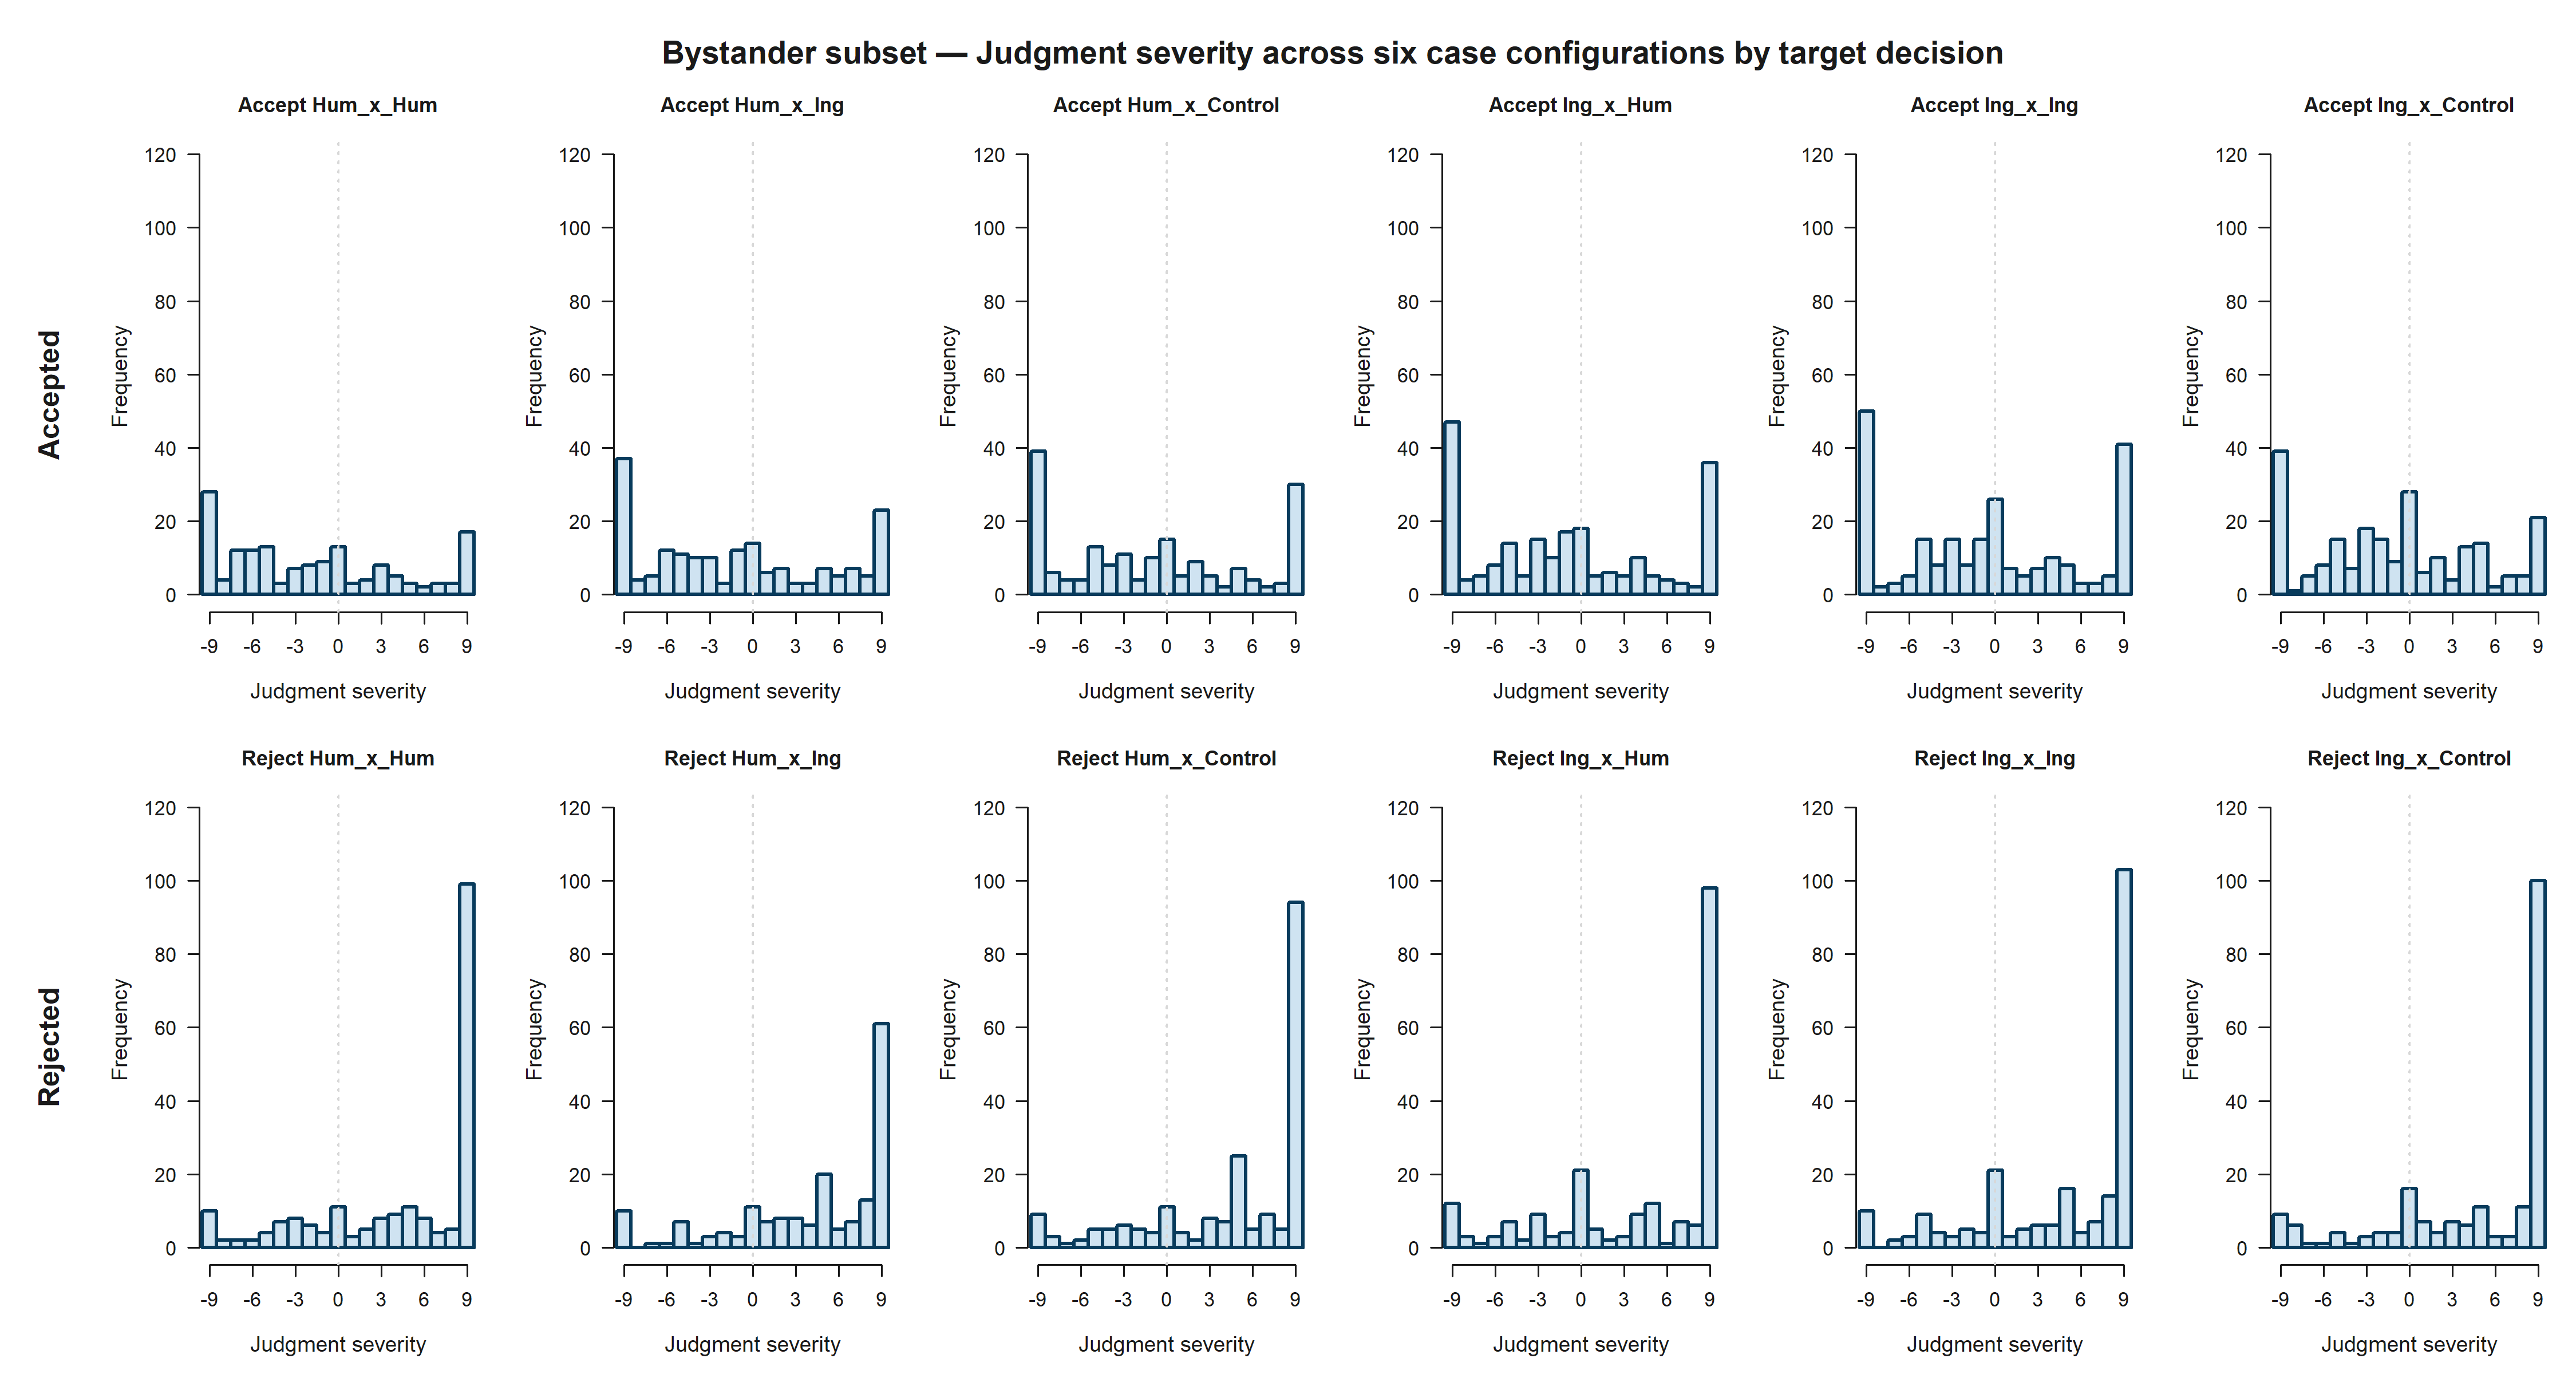
\includegraphics[width=0.92\textwidth]{../figures/figure_07_bystander_subset_judgment_distributions_across_six_case_configurations.png}
\caption{Bystander-subset judgment distributions across the six explicit victim x negotiator faculty configurations, with separate rows for accepted and rejected harmful deals, scale $-9$ to $9$.}
\label{fig:bystander_case_panels}
\end{figure}
\begin{figure}[H]
\centering
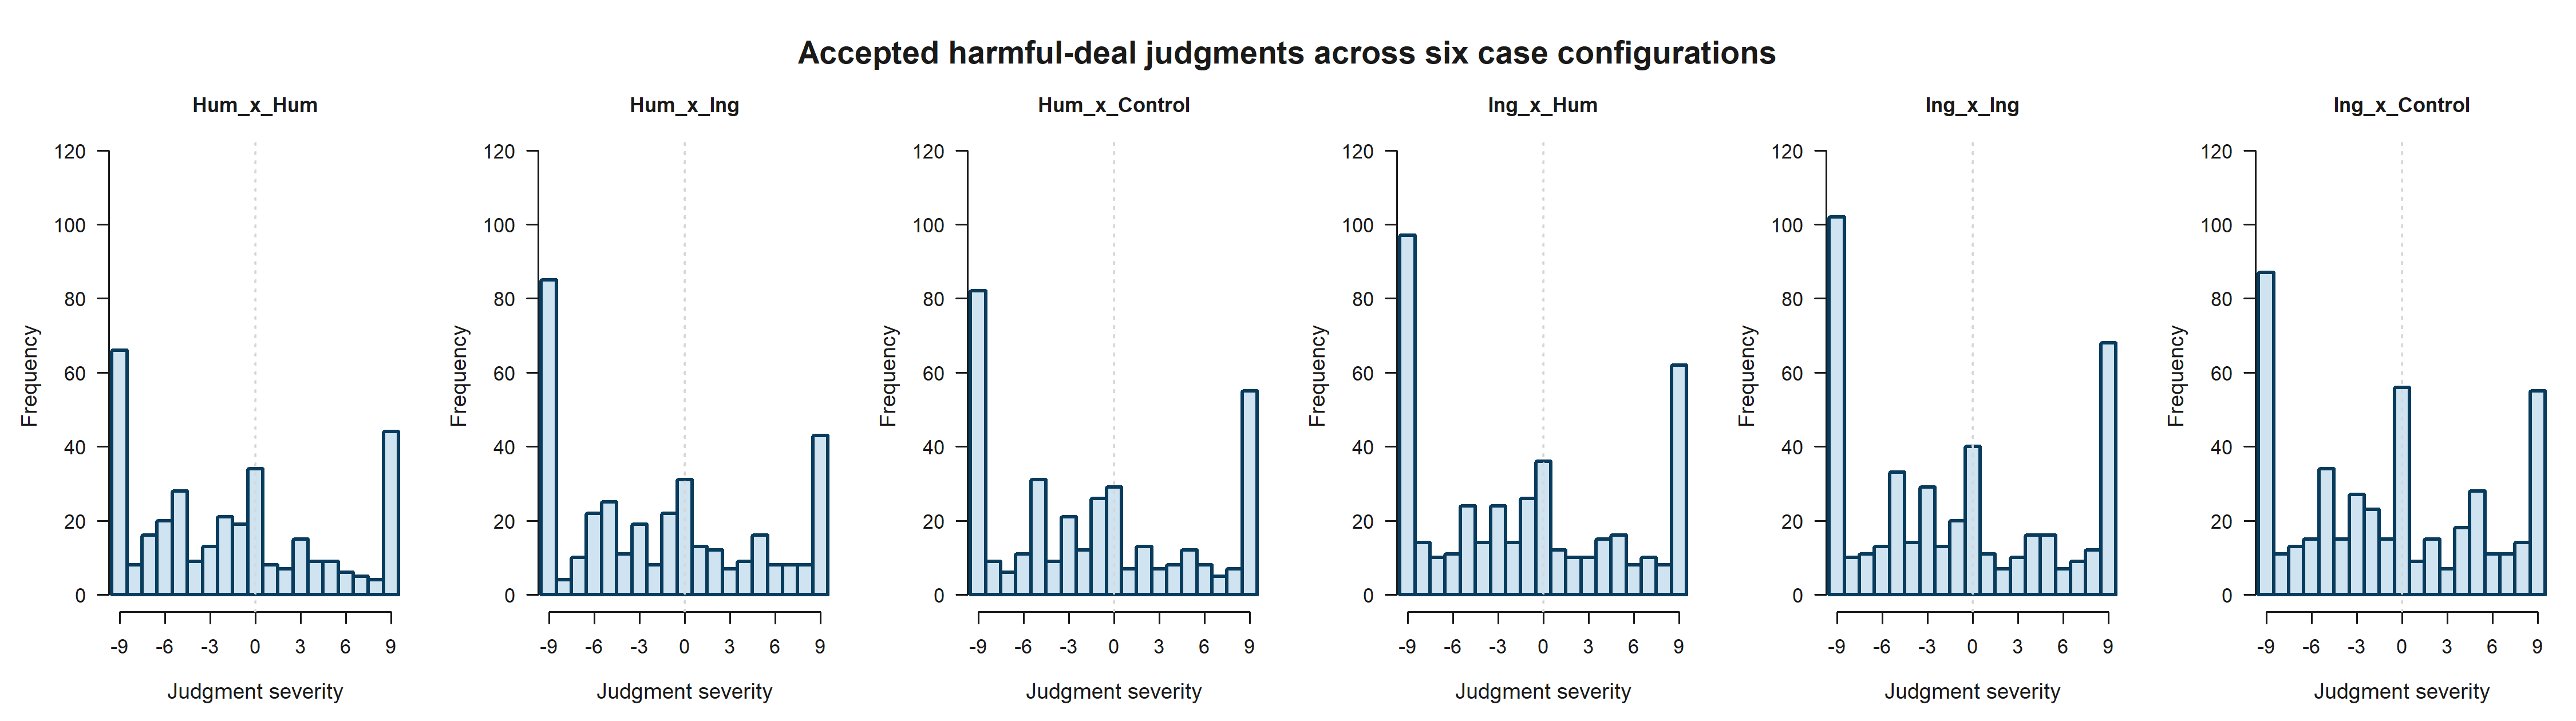
\includegraphics[width=0.92\textwidth]{../figures/figure_08_accepted_harmful_deal_judgment_distributions_across_six_case_configurations.png}
\caption{Accepted harmful-deal judgments across the six explicit victim x negotiator faculty configurations in the full analytical sample, scale $-9$ to $9$.}
\label{fig:accepted_case_panels}
\end{figure}
\begin{figure}[H]
\centering
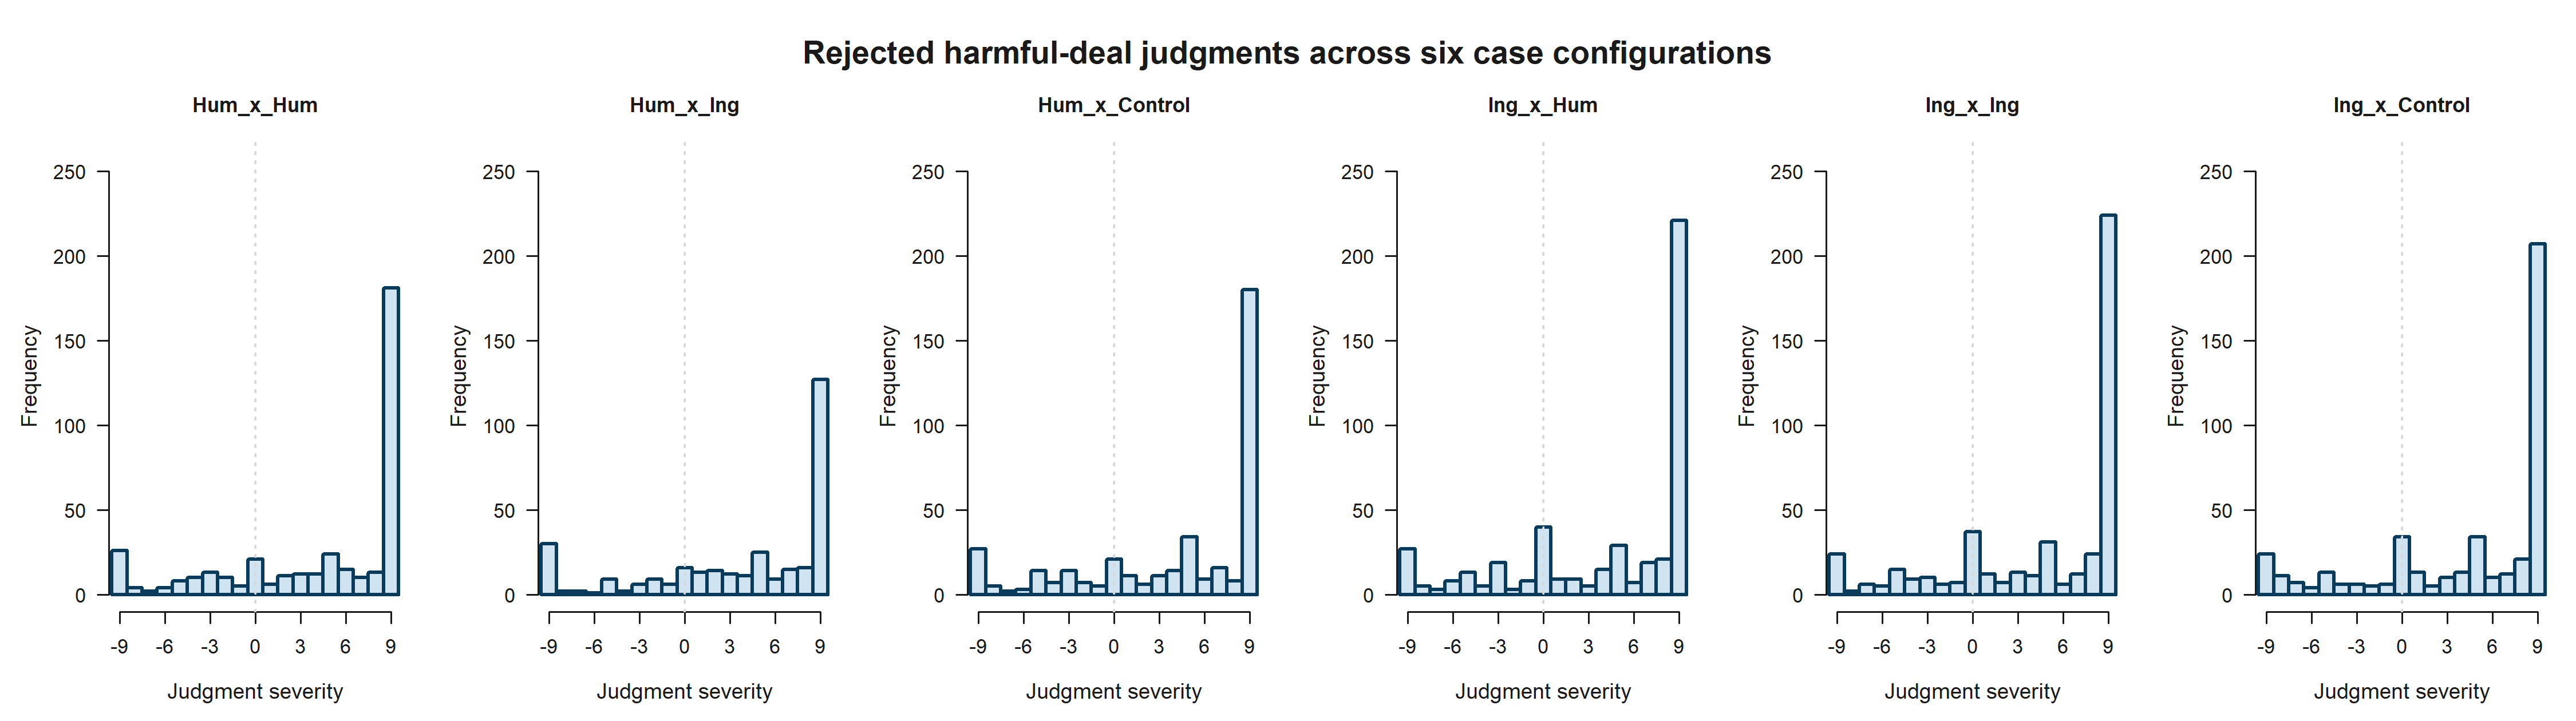
\includegraphics[width=0.92\textwidth]{../figures/figure_09_rejected_harmful_deal_judgment_distributions_across_six_case_configurations.png}
\caption{Rejected harmful-deal judgments across the six explicit victim x negotiator faculty configurations in the full analytical sample, scale $-9$ to $9$.}
\label{fig:rejected_case_panels}
\end{figure}
When a control-labeled negotiator condition exists, the active hypothesis models treat that control level as the reference category. Observer--victim alignment remains binary and therefore keeps ingroup as its reference level.

\section{Bi-variate Statistics}
The correlation matrix between the psychometric subscales and the mean moral judgment is presented below. Figure \ref{fig:bivariate_scatters} complements that matrix with participant-level scatterplots, fitted lines, and 95\% confidence bands on the observed judgment scale.
\begin{table}[H]
\centering
\caption{Correlation Matrix: IRI Subscales and Moral Judgment.}
\label{tab:bivar}
\resizebox{\textwidth}{!}{%
\begin{tabular}{lllll}
\toprule
Fantasy & Empathic Concern & Perspective Taking & Personal Distress & Mean Judgment \\
\midrule
1.000 & 0.476 & 0.524 & 0.490 & -0.062 \\
0.476 & 1.000 & 0.402 & 0.598 & -0.150 \\
0.524 & 0.402 & 1.000 & 0.265 & 0.008 \\
0.490 & 0.598 & 0.265 & 1.000 & -0.003 \\
-0.062 & -0.150 & 0.008 & -0.003 & 1.000 \\
\bottomrule
\end{tabular}
}
\end{table}
\begin{figure}[H]
\centering
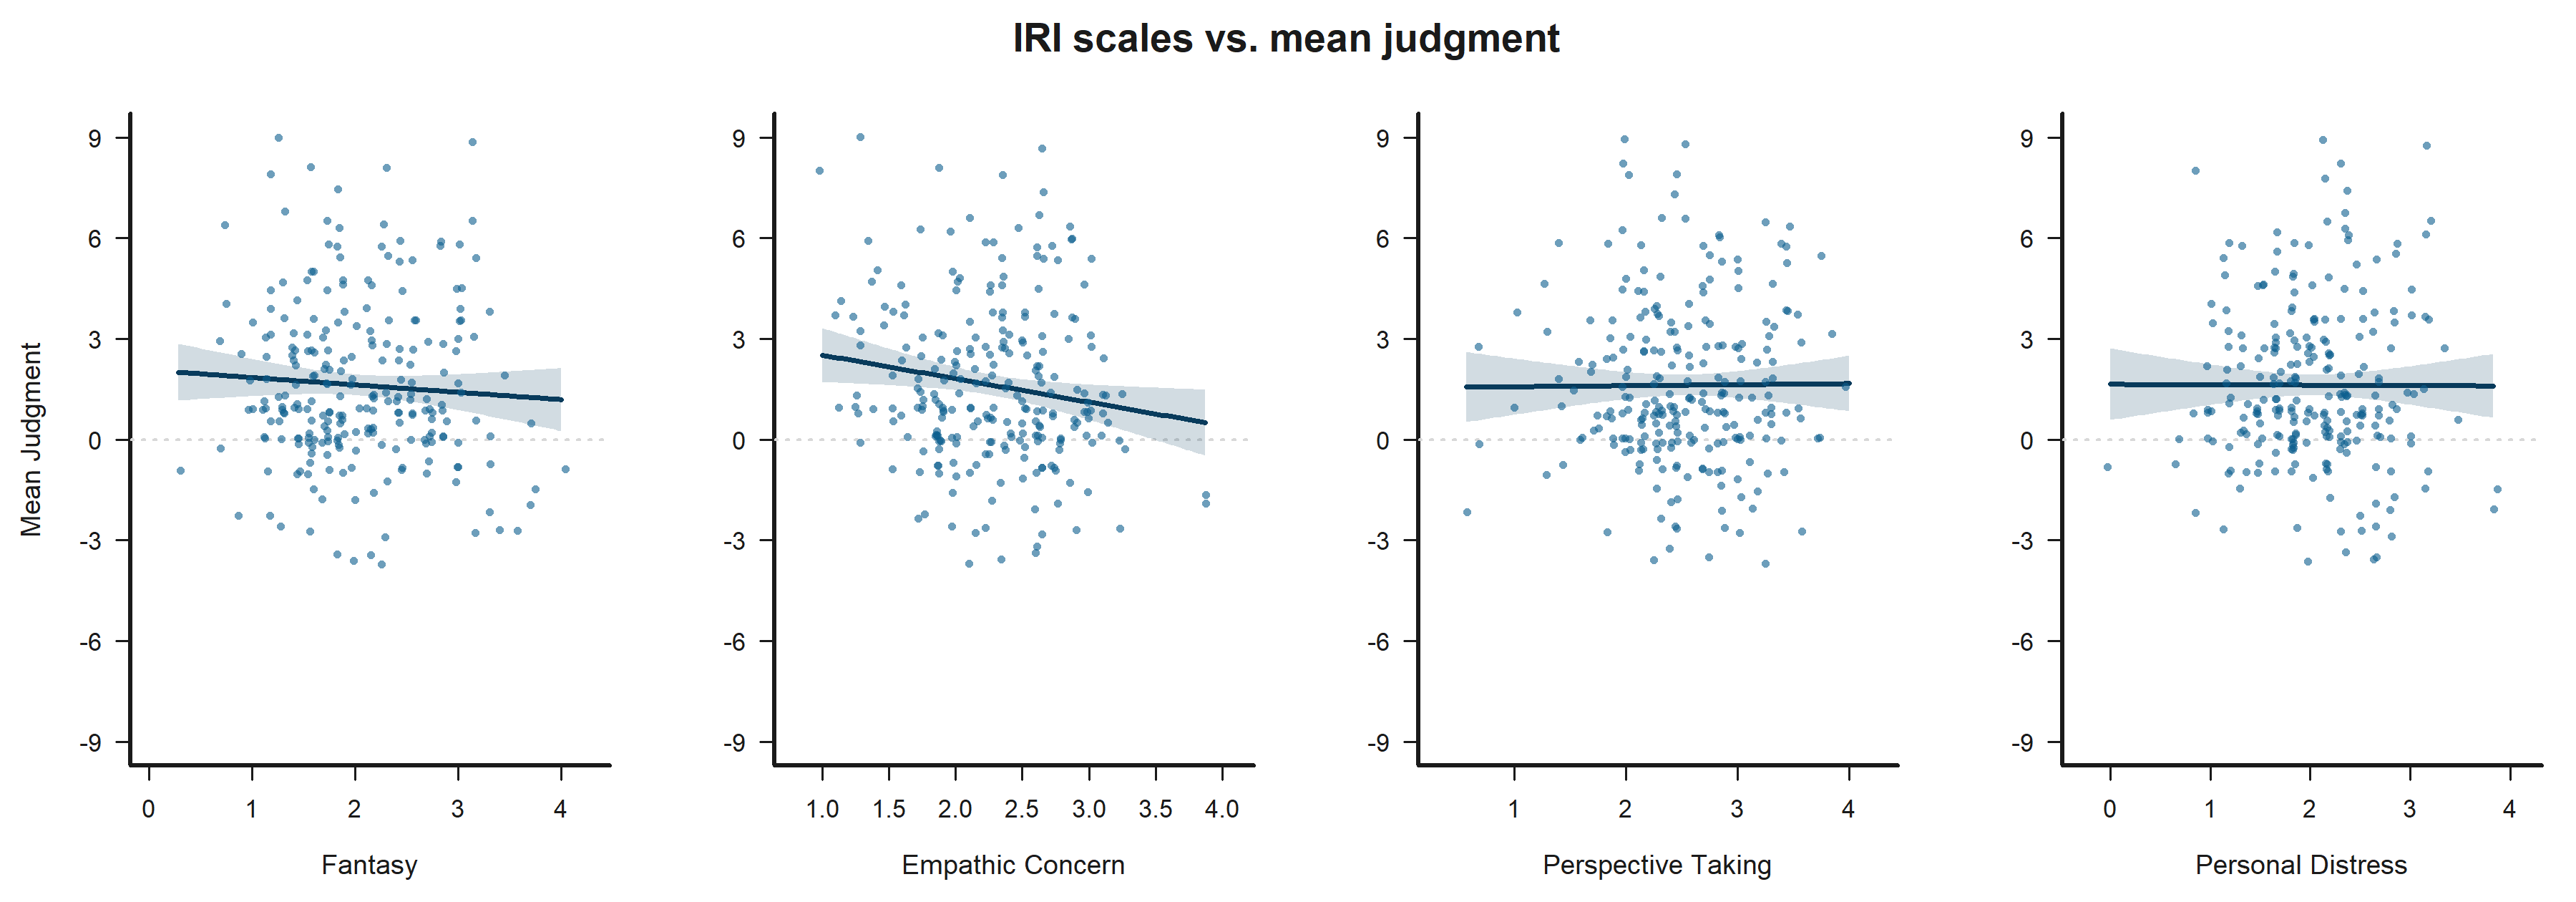
\includegraphics[width=0.92\textwidth]{../figures/figure_05_bivariate_scatters_iri_scales_vs_mean_judgment.png}
\caption{Bivariate scatters of participant-level IRI scales versus mean judgment, with fitted lines and 95\% confidence bands. The judgment axis is fixed at $-9$ to $9$.}
\label{fig:bivariate_scatters}
\end{figure}

\section{Estimator Fit Summary}
The following table consolidates fit-status information for the Tobit models with random intercepts used in this report.
\begin{table}[H]
\centering
{\fontsize{11}{13}\selectfont
\renewcommand{\arraystretch}{1.10}
\caption{Estimator fit summary across Tobit-random-intercepts specifications.}
\label{tab:model_fit_summary}
\begin{tabularx}{\textwidth}{>{\raggedright\arraybackslash}Xllllllll}
\toprule
Hypothesis & Subset & Specification & Approach & Status & Iterations & Observations & Participants & Cluster unit \\
\midrule
H1 & Bystander & Model B & Tobit & Completed & -- & 2430 & 243 & case + participant \\
H1 & Victim & Model B & Tobit & Completed & -- & 2430 & 243 & case + participant \\
H2 & Bystander & Model B & Tobit & Completed & -- & 2430 & 243 & case + participant \\
H2 & Victim & Model B & Tobit & Completed & -- & 2430 & 243 & case + participant \\
H3 & Bystander & Model B & Tobit & Completed & -- & 2430 & 243 & case + participant \\
H3 & Victim & Model B & Tobit & Completed & -- & 2430 & 243 & case + participant \\
\bottomrule
\end{tabularx}
}
\end{table}
\begin{flushleft}
\footnotesize\textit{Note.} Reported approaches: Tobit. Iterations are shown as -- when the saved estimator object does not report a comparable iteration count. Cluster unit entries used in this table: case + participant.
\end{flushleft}

\subsection{Hypothesis Significance Summary}
The following concise tables list only hypothesis-relevant predictors that reached at least p < 0.10 in the available Tobit models with random intercepts, split by victim and bystander subsets, using conventional symbols to indicate strength of evidence (plus for p < 0.10, one-star for p < 0.05, two-star for p < 0.01, and three-star for p < 0.001). Dynamic figures are generated only for predictors that appear in these tables with at least one significance symbol.
\paragraph{Victim subset}
\begin{table}[H]
\centering
{\fontsize{11}{13}\selectfont
\renewcommand{\arraystretch}{1.15}
\caption{Hypothesis-level significance summary for the victim subset across Tobit random-intercepts models.}
\label{tab:hypothesis_summary_victim}
\begin{tabular}{>{\raggedright\arraybackslash}p{0.12\textwidth}>{\raggedright\arraybackslash}p{0.74\textwidth}}
\toprule
Hypothesis & Tobit (random intercepts) support \\
\midrule
H1 & PT* \\
H2 & None \\
H3 & PT x V-N1 Out*;\newline EC x V-N1 Out* \\
\bottomrule
\end{tabular}
}
\end{table}
\begin{flushleft}
\footnotesize\textit{Note.} Abbrev.: EC = empathic concern; PT = perspective taking; N1 = judged negotiator; V-N1 = victim-negotiator 1 relation.
\end{flushleft}

\paragraph{Bystander subset}
\begin{table}[H]
\centering
{\fontsize{11}{13}\selectfont
\renewcommand{\arraystretch}{1.15}
\caption{Hypothesis-level significance summary for the bystander subset across Tobit random-intercepts models.}
\label{tab:hypothesis_summary_bystander}
\begin{tabular}{>{\raggedright\arraybackslash}p{0.12\textwidth}>{\raggedright\arraybackslash}p{0.74\textwidth}}
\toprule
Hypothesis & Tobit (random intercepts) support \\
\midrule
H1 & None \\
H2 & B-V Out*;\newline V-N2 In+;\newline B-N2 Out+;\newline B-N2 In+;\newline B-N1 In x B-N2 In+ \\
H3 & B-N1 Out x FS*;\newline B-V Out x PD+;\newline B-N2 Out x PT+ \\
\bottomrule
\end{tabular}
}
\end{table}
\begin{flushleft}
\footnotesize\textit{Note.} Abbrev.: FS = fantasy; PT = perspective taking; PD = personal distress; N1 = judged negotiator; N2 = counterpart negotiator; B-V = bystander-victim relation; V-N2 = victim-negotiator 2 relation; B-N1 = bystander-negotiator 1 relation; B-N2 = bystander-negotiator 2 relation.
\end{flushleft}


\subsection{Significance-Driven Figures}
Only hypothesis-relevant predictors that reach p < 0.10 or better are visualized automatically. These dynamic figures use the saved Tobit random-intercepts outputs, and participant id remains only an inference-level clustering unit rather than a substantive explanatory variable.

\paragraph{Empathy Effect}

Empathy: Perspective taking is statistically significant in the Tobit random-intercepts model (*, p = 0.017). Figure \ref{fig:sig_H1_iri_pt} shows that across the observed range, higher Empathy: Perspective taking corresponds to higher predicted judgment.

\begin{figure}[H]
\centering
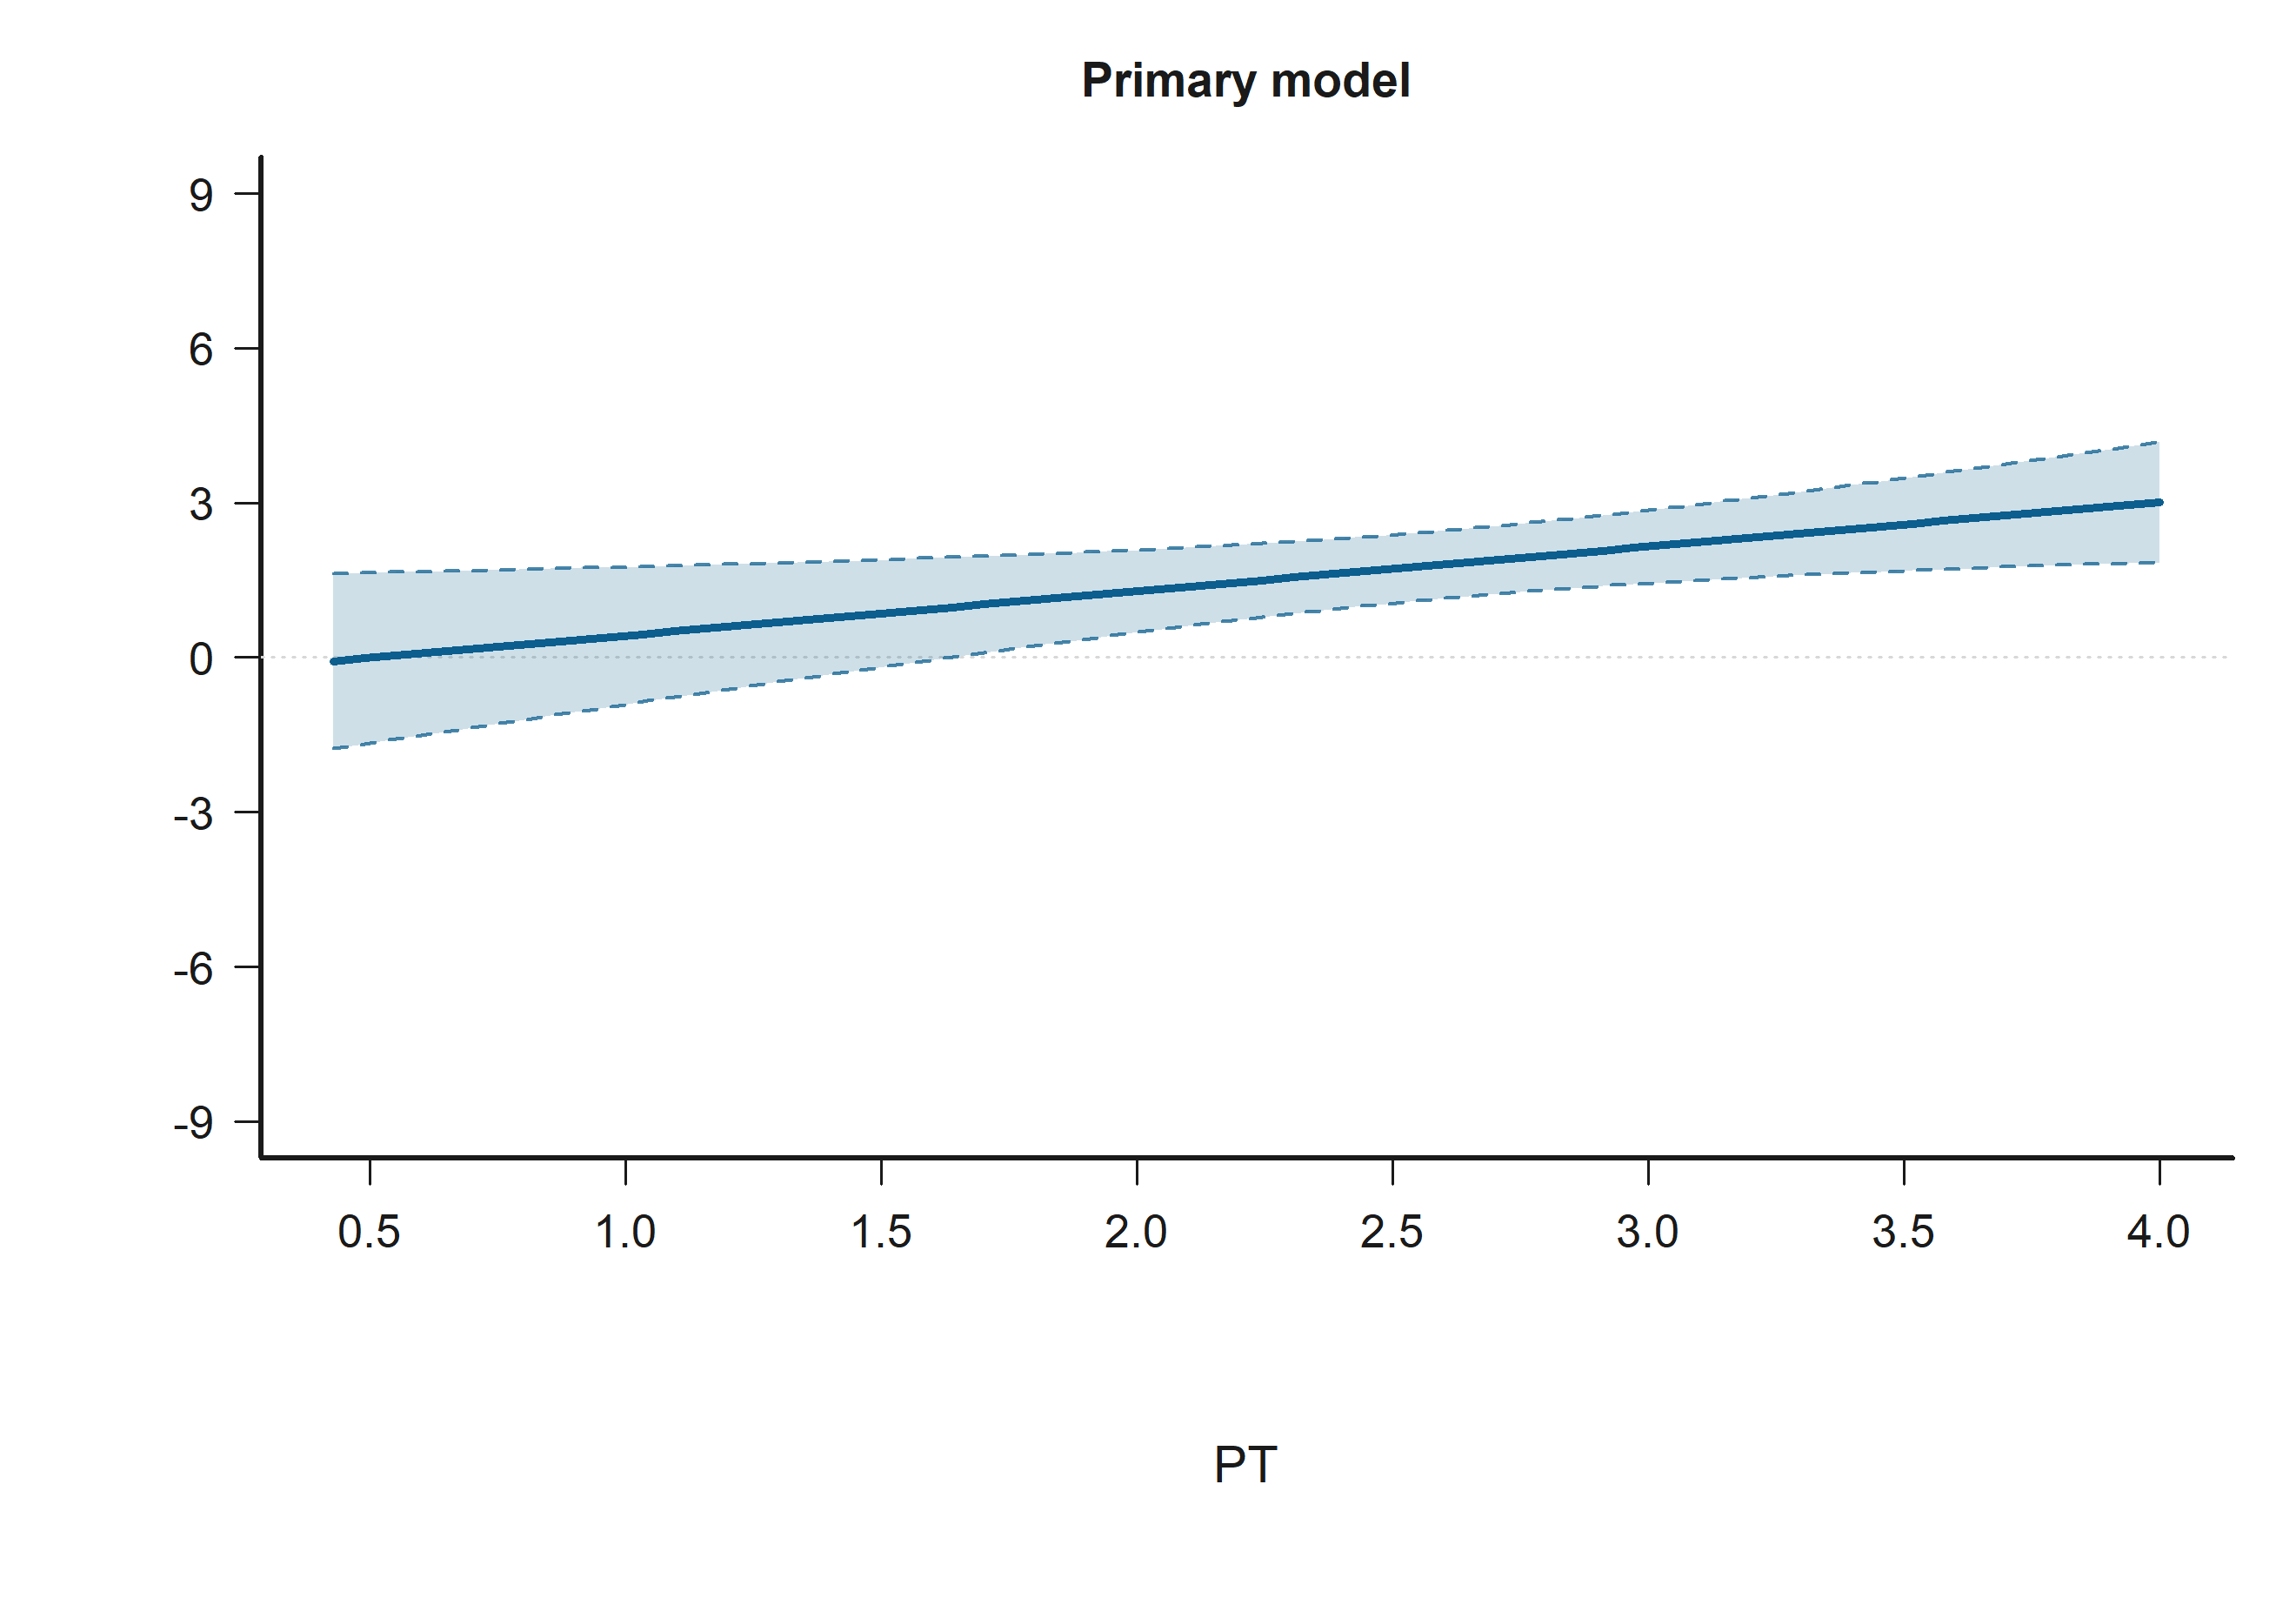
\includegraphics[width=0.92\textwidth]{../figures/figure_sig_H1_iri_pt_h1_empathy_perspective_taking.png}
\caption{Effect Plot for Empathy: Perspective taking in Empathy Effect. The panels show predicted judgments on the observed -9 to 9 scale with 95\% confidence intervals. Abbrev.: FS / EC / PT / PD = IRI subscales; N1 / N2 = negotiator 1 / negotiator 2; B-V = bystander-victim relation; V-N1 / V-N2 = victim-negotiator relations; B-N1 / B-N2 = bystander-negotiator relations; Vic / Obs = victim / observer subset; In / Out / Ctl = ingroup / outgroup / control label hidden; SameFac = N1 and N2 same faculty; SES = economic status.}
\label{fig:sig_H1_iri_pt}
\end{figure}

\paragraph{Negotiator-Side Structure}

Bystander-victim: Outgroup (ref = Ingroup) is statistically significant in the Tobit random-intercepts model (*, p = 0.035). Figure \ref{fig:sig_H2_bystander_victim_groupout} shows that predicted judgment is lower for B-V Out than for B-V In.

\begin{figure}[H]
\centering
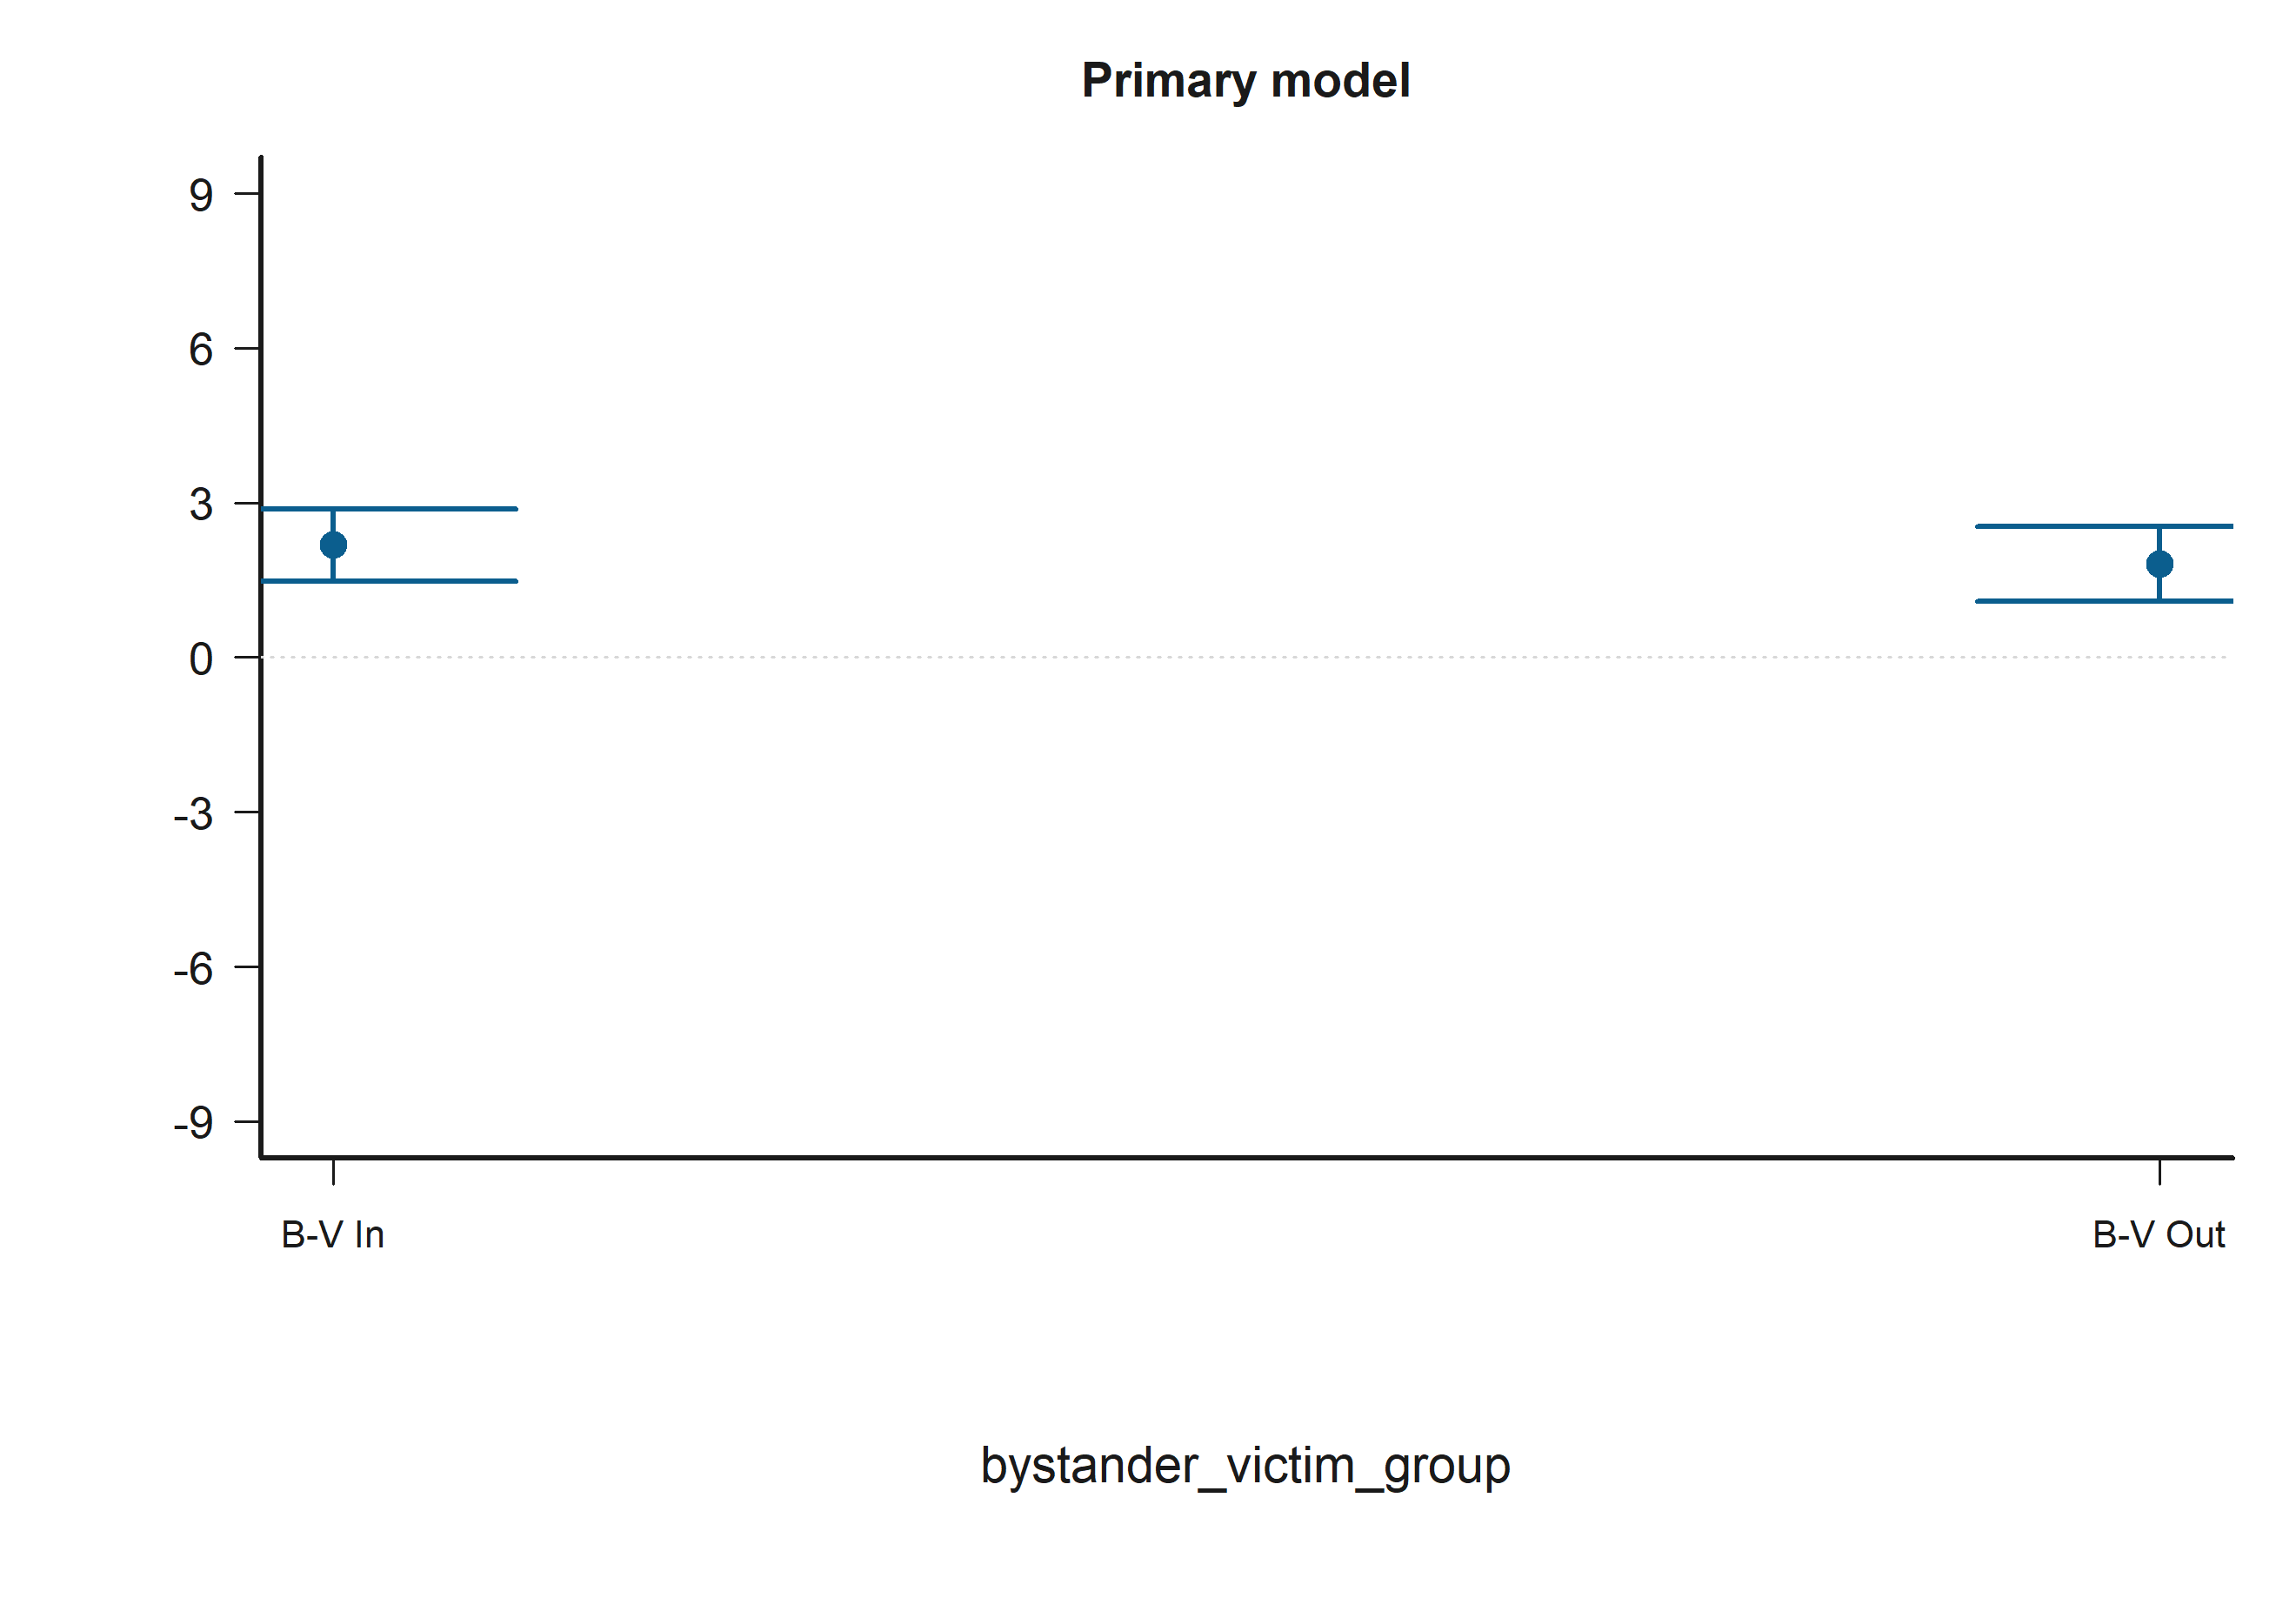
\includegraphics[width=0.92\textwidth]{../figures/figure_sig_H2_bystander_victim_groupout_h2_bystander_victim_outgroup_ref_ingroup.png}
\caption{Grouped Prediction Plot for Bystander-victim: Outgroup (ref = Ingroup) in Negotiator-Side Structure. The panels show predicted judgments on the observed -9 to 9 scale with 95\% confidence intervals. Abbrev.: FS / EC / PT / PD = IRI subscales; N1 / N2 = negotiator 1 / negotiator 2; B-V = bystander-victim relation; V-N1 / V-N2 = victim-negotiator relations; B-N1 / B-N2 = bystander-negotiator relations; Vic / Obs = victim / observer subset; In / Out / Ctl = ingroup / outgroup / control label hidden; SameFac = N1 and N2 same faculty; SES = economic status.}
\label{fig:sig_H2_bystander_victim_groupout}
\end{figure}

Victim-N2: Ingroup (ref = Control) is statistically significant in the Tobit random-intercepts model (+, p = 0.071). Figure \ref{fig:sig_H2_victim_n2_groupin} shows that predicted judgment is higher for V-N2 In than for V-N2 Ctl.

\begin{figure}[H]
\centering
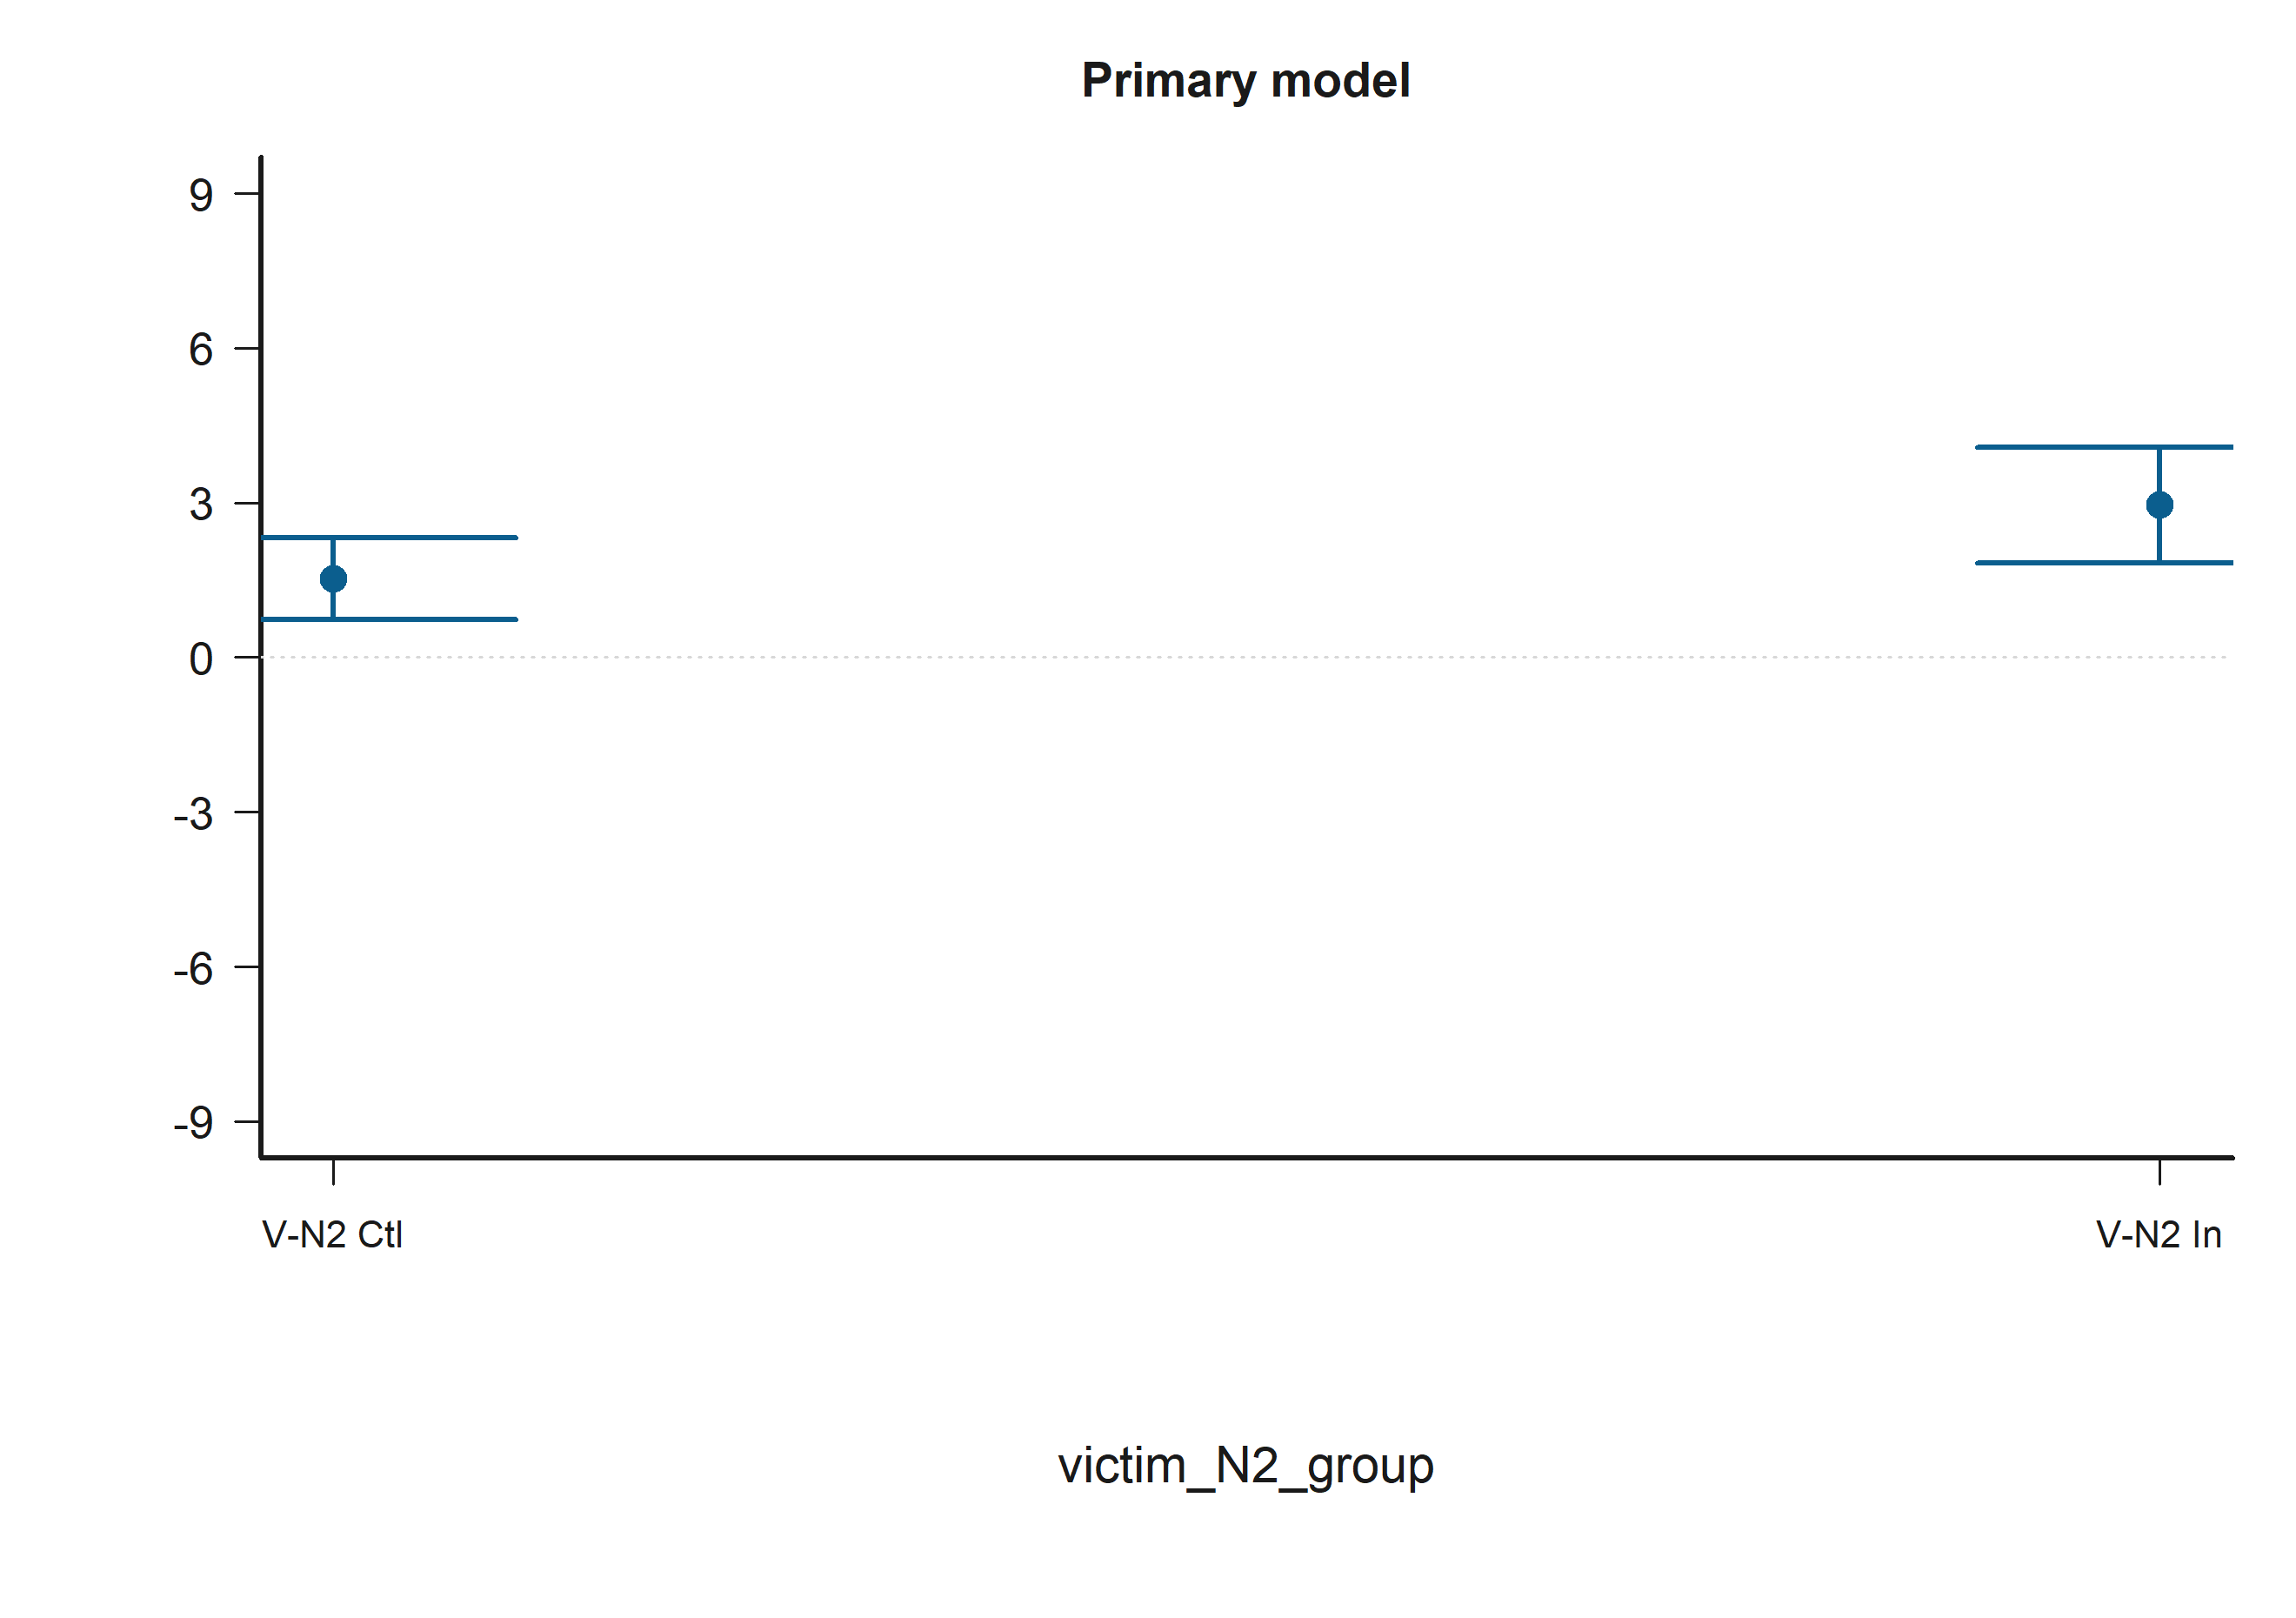
\includegraphics[width=0.92\textwidth]{../figures/figure_sig_H2_victim_n2_groupin_h2_victim_n2_ingroup_ref_control.png}
\caption{Grouped Prediction Plot for Victim-N2: Ingroup (ref = Control) in Negotiator-Side Structure. The panels show predicted judgments on the observed -9 to 9 scale with 95\% confidence intervals. Abbrev.: FS / EC / PT / PD = IRI subscales; N1 / N2 = negotiator 1 / negotiator 2; B-V = bystander-victim relation; V-N1 / V-N2 = victim-negotiator relations; B-N1 / B-N2 = bystander-negotiator relations; Vic / Obs = victim / observer subset; In / Out / Ctl = ingroup / outgroup / control label hidden; SameFac = N1 and N2 same faculty; SES = economic status.}
\label{fig:sig_H2_victim_n2_groupin}
\end{figure}

Bystander-N2: Outgroup (ref = Control) is statistically significant in the Tobit random-intercepts model (+, p = 0.073). Figure \ref{fig:sig_H2_bystander_n2_groupout} shows that predicted judgment is lower for B-N2 Out than for B-N2 Ctl.

\begin{figure}[H]
\centering
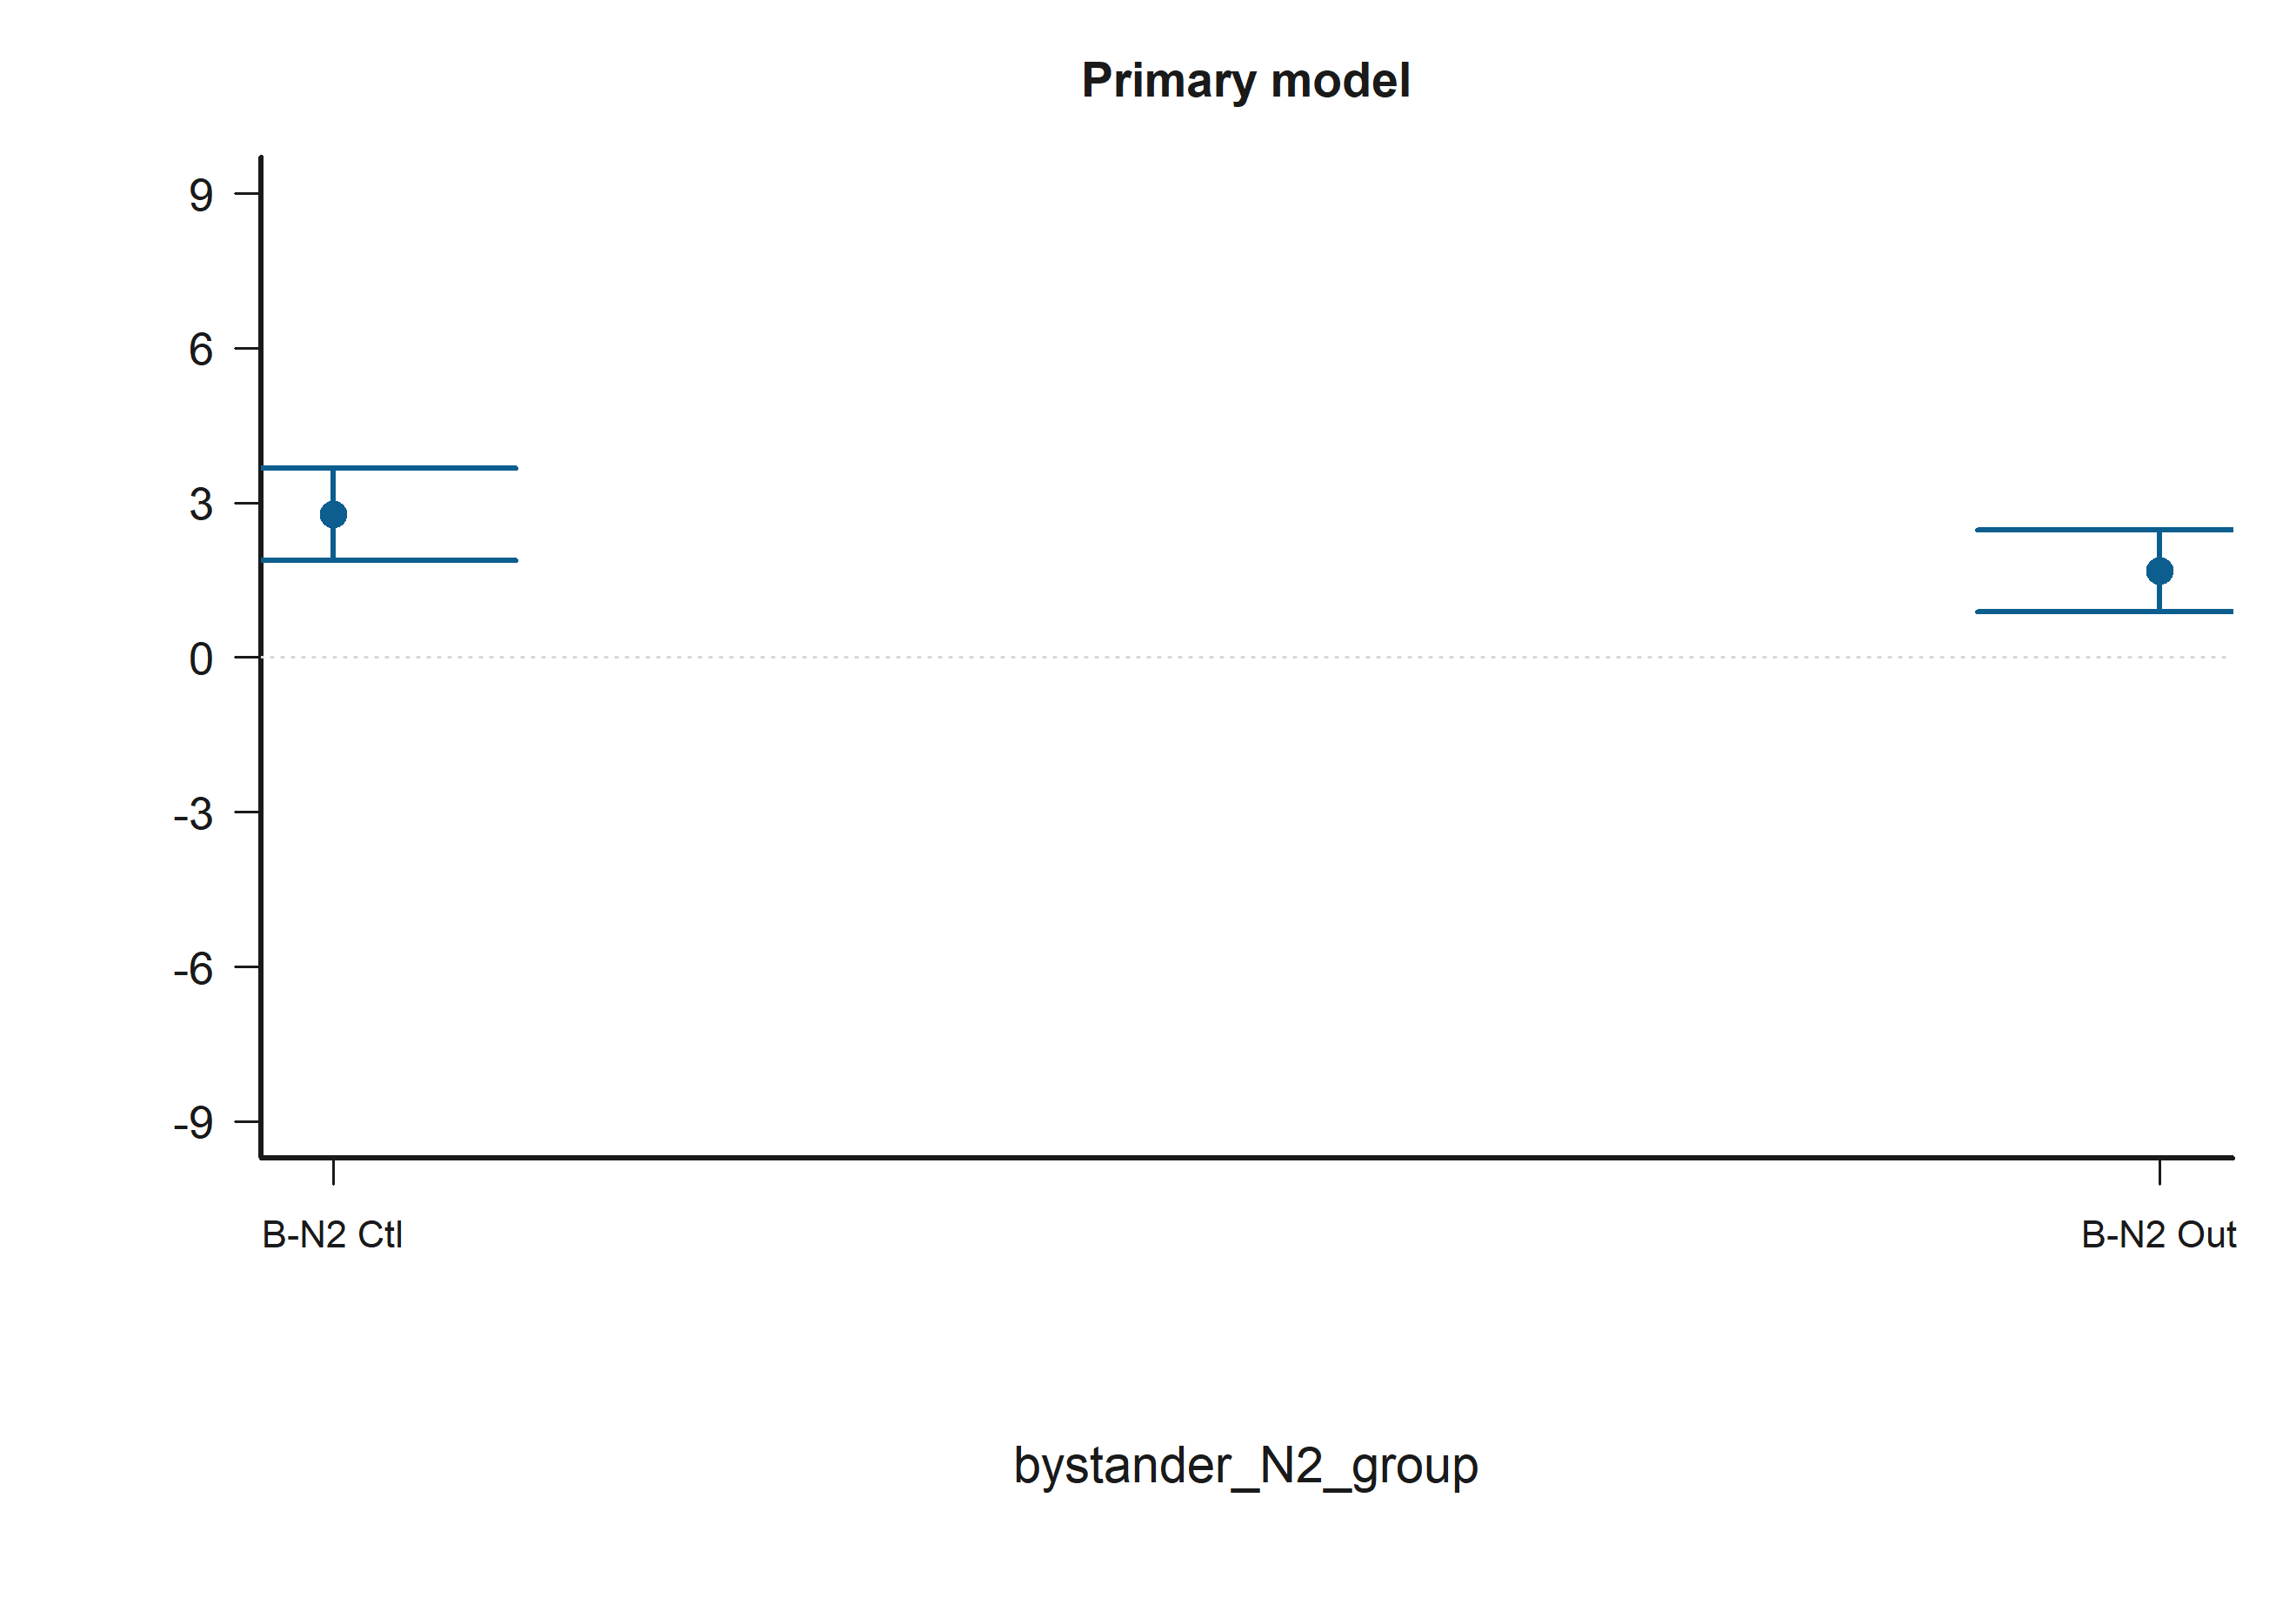
\includegraphics[width=0.92\textwidth]{../figures/figure_sig_H2_bystander_n2_groupout_h2_bystander_n2_outgroup_ref_control.png}
\caption{Grouped Prediction Plot for Bystander-N2: Outgroup (ref = Control) in Negotiator-Side Structure. The panels show predicted judgments on the observed -9 to 9 scale with 95\% confidence intervals. Abbrev.: FS / EC / PT / PD = IRI subscales; N1 / N2 = negotiator 1 / negotiator 2; B-V = bystander-victim relation; V-N1 / V-N2 = victim-negotiator relations; B-N1 / B-N2 = bystander-negotiator relations; Vic / Obs = victim / observer subset; In / Out / Ctl = ingroup / outgroup / control label hidden; SameFac = N1 and N2 same faculty; SES = economic status.}
\label{fig:sig_H2_bystander_n2_groupout}
\end{figure}

Bystander-N2: Ingroup (ref = Control) is statistically significant in the Tobit random-intercepts model (+, p = 0.083). Figure \ref{fig:sig_H2_bystander_n2_groupin} shows that predicted judgment is lower for B-N2 In than for B-N2 Ctl.

\begin{figure}[H]
\centering
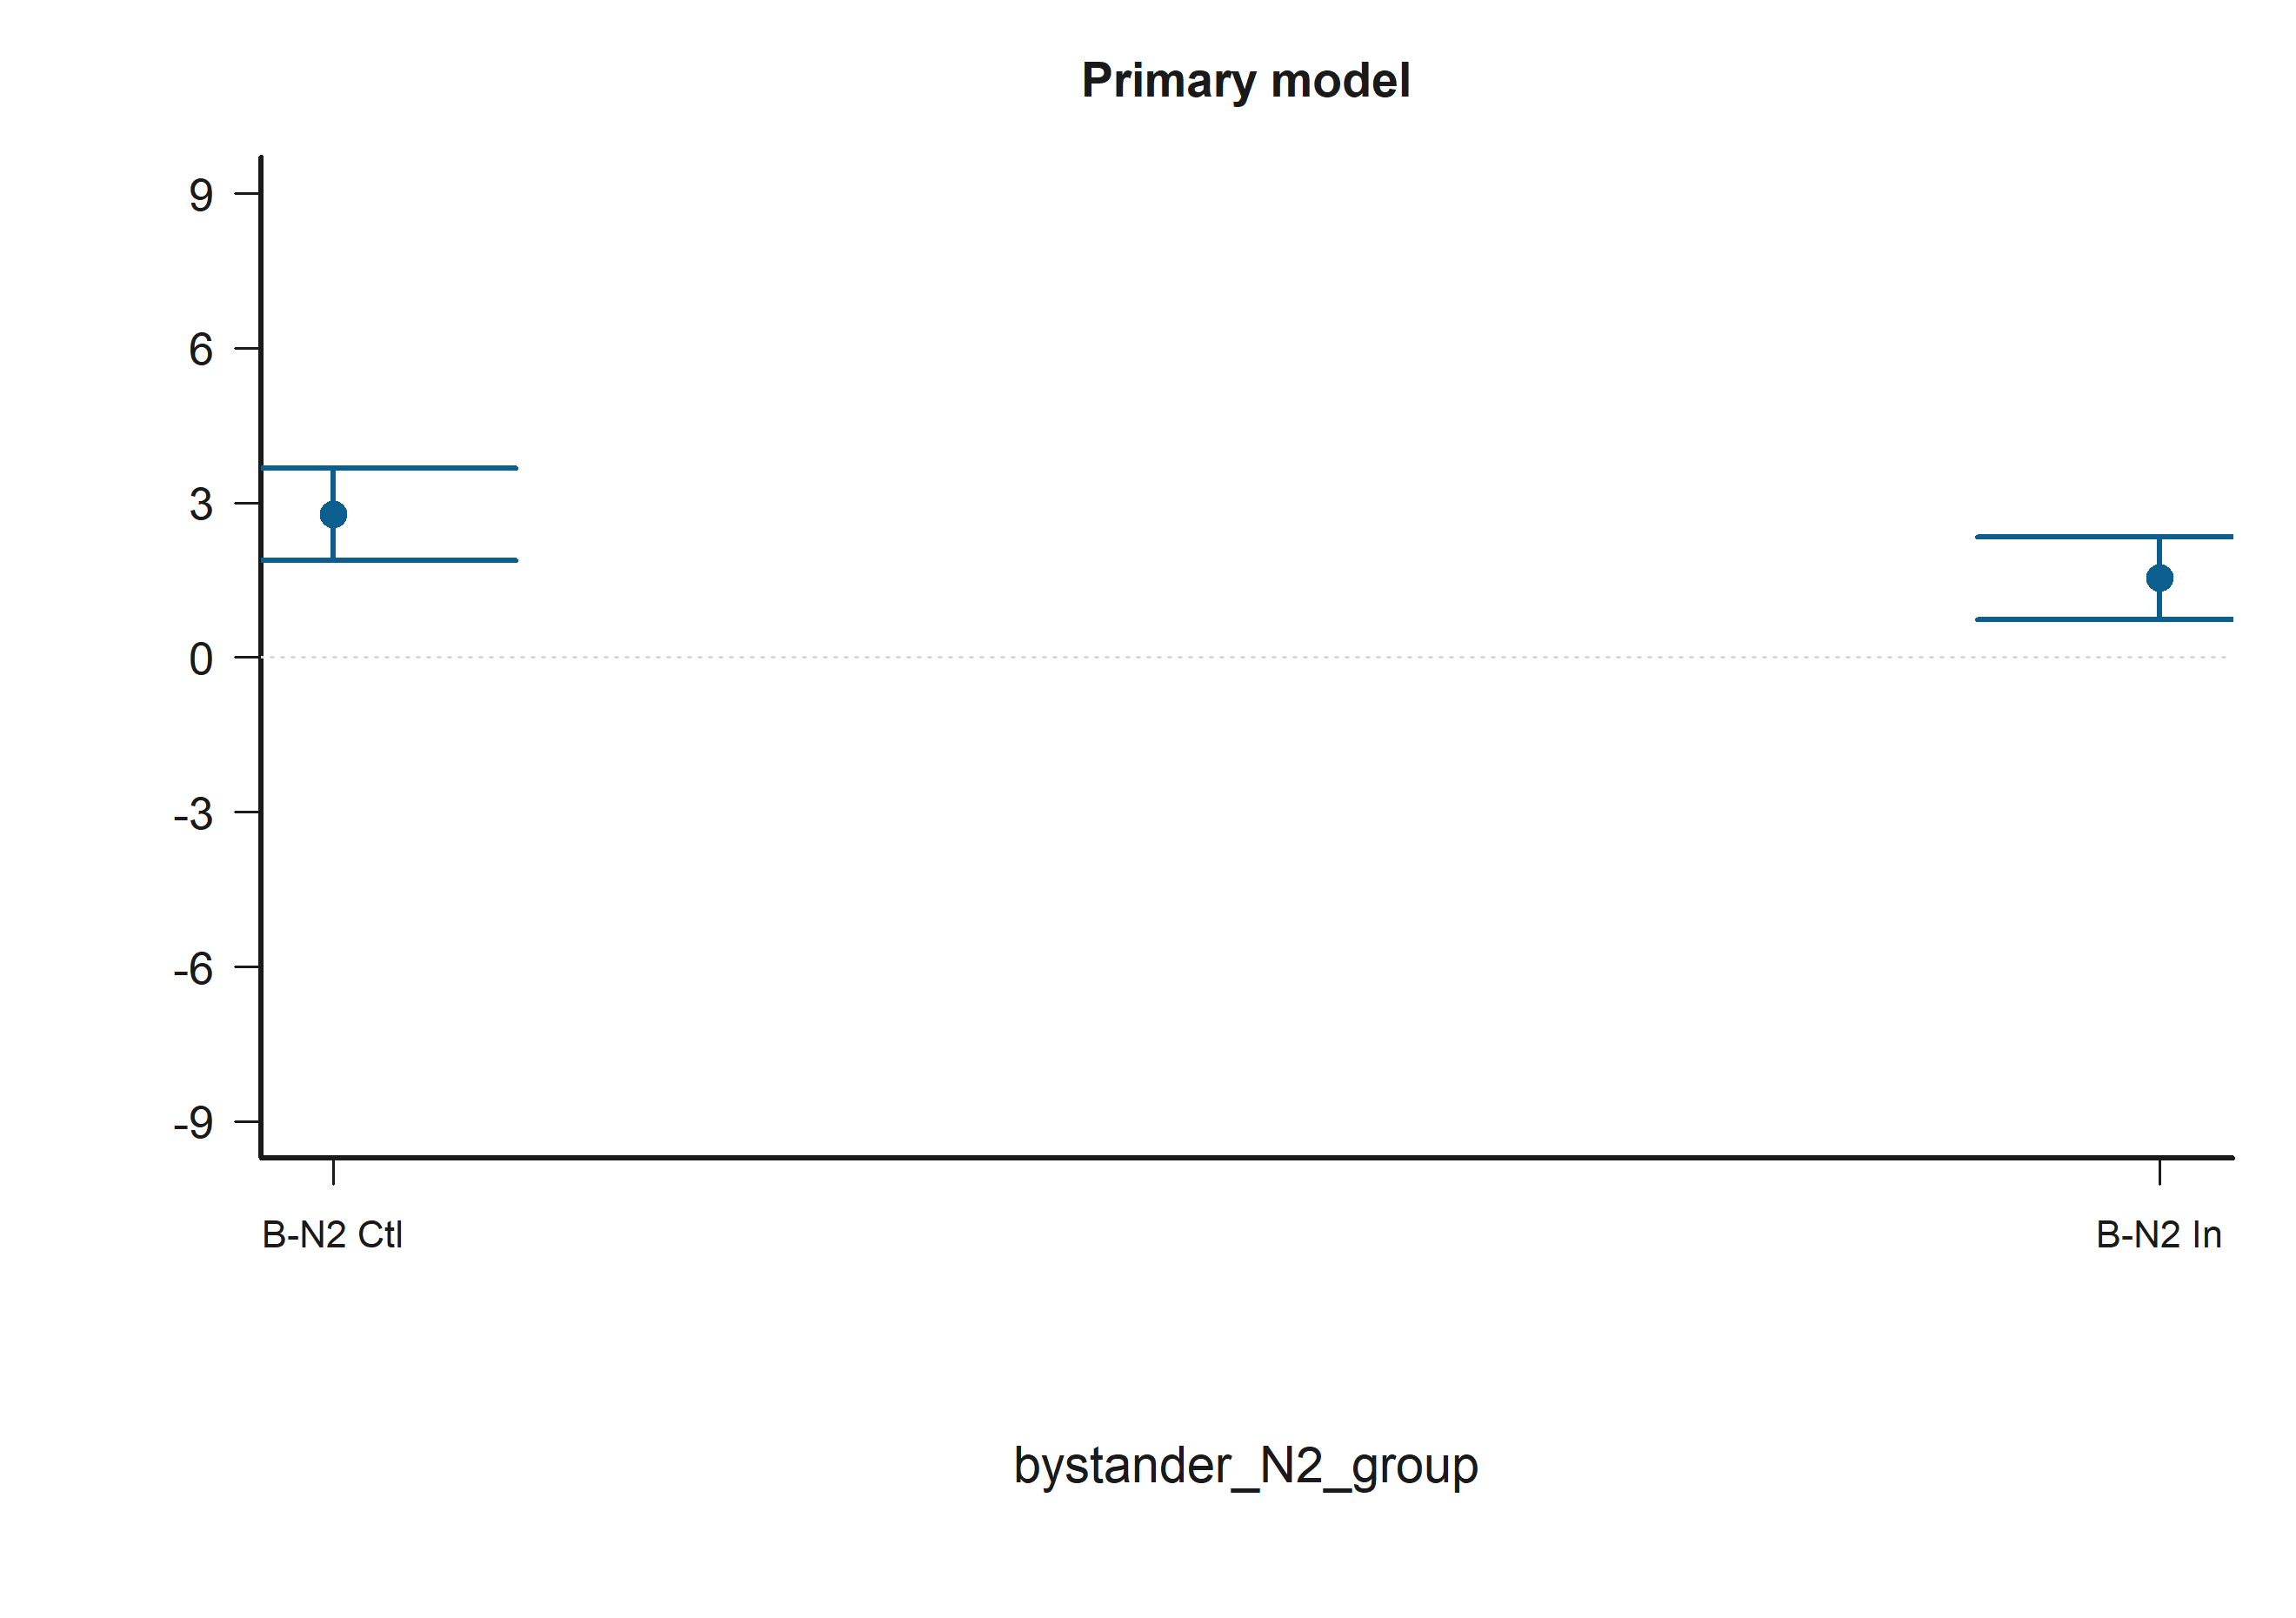
\includegraphics[width=0.92\textwidth]{../figures/figure_sig_H2_bystander_n2_groupin_h2_bystander_n2_ingroup_ref_control.png}
\caption{Grouped Prediction Plot for Bystander-N2: Ingroup (ref = Control) in Negotiator-Side Structure. The panels show predicted judgments on the observed -9 to 9 scale with 95\% confidence intervals. Abbrev.: FS / EC / PT / PD = IRI subscales; N1 / N2 = negotiator 1 / negotiator 2; B-V = bystander-victim relation; V-N1 / V-N2 = victim-negotiator relations; B-N1 / B-N2 = bystander-negotiator relations; Vic / Obs = victim / observer subset; In / Out / Ctl = ingroup / outgroup / control label hidden; SameFac = N1 and N2 same faculty; SES = economic status.}
\label{fig:sig_H2_bystander_n2_groupin}
\end{figure}

Bystander-N1: Ingroup (ref = Control) x Bystander-N2: Ingroup (ref = Control) is statistically significant in the Tobit random-intercepts model (+, p = 0.098). Figure \ref{fig:sig_H2_bystander_n1_groupin_bystander_n2_groupin} shows that the predicted relationship rises most sharply for bystander\_N1\_group when the condition is B-N2 Ctl.

\begin{figure}[H]
\centering
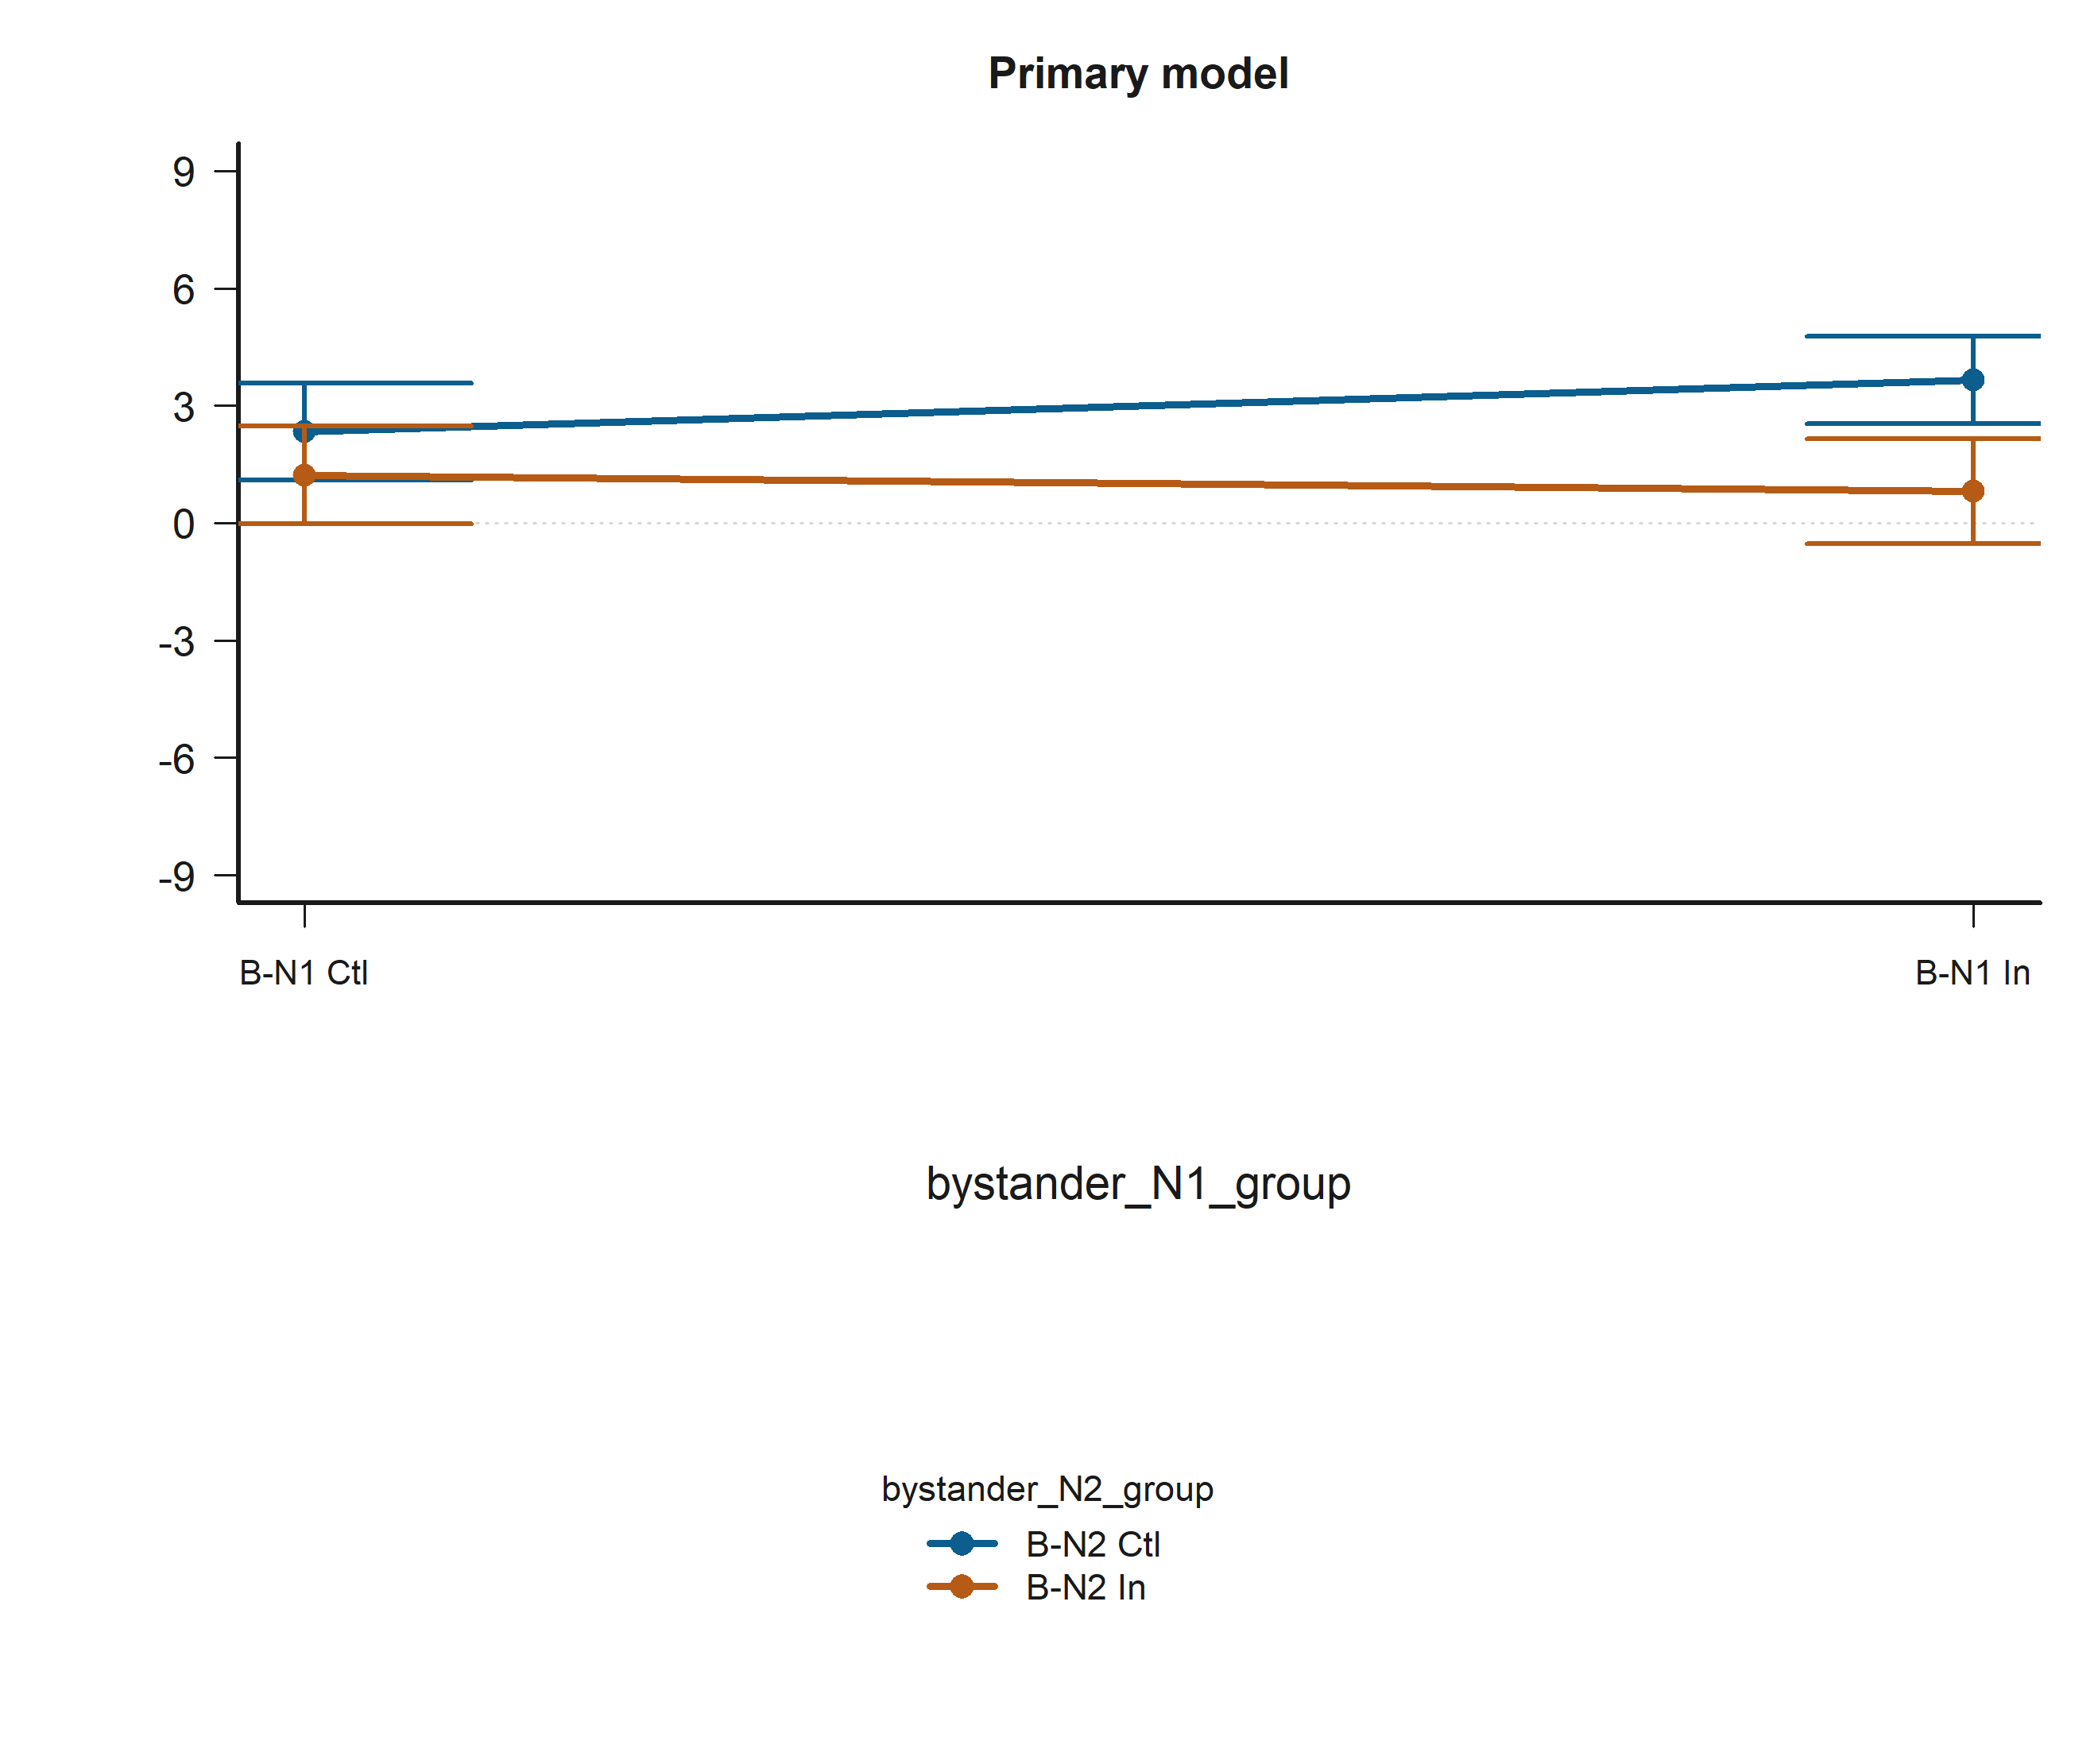
\includegraphics[width=0.92\textwidth]{../figures/figure_sig_H2_bystander_n1_groupin_bystander_n2_groupin_h2_bystander_n1_ingroup_ref_control_x_bystander_n2_ingroup_ref_control.png}
\caption{Interaction Plot for Bystander-N1: Ingroup (ref = Control) x Bystander-N2: Ingroup (ref = Control) in Negotiator-Side Structure. The panels show predicted judgments on the observed -9 to 9 scale with 95\% confidence intervals. Abbrev.: FS / EC / PT / PD = IRI subscales; N1 / N2 = negotiator 1 / negotiator 2; B-V = bystander-victim relation; V-N1 / V-N2 = victim-negotiator relations; B-N1 / B-N2 = bystander-negotiator relations; Vic / Obs = victim / observer subset; In / Out / Ctl = ingroup / outgroup / control label hidden; SameFac = N1 and N2 same faculty; SES = economic status.}
\label{fig:sig_H2_bystander_n1_groupin_bystander_n2_groupin}
\end{figure}

\paragraph{Empathy x Relational Status}

Empathy: Perspective taking x Victim-N1: Outgroup (ref = Control) is statistically significant in the Tobit random-intercepts model (*, p = 0.014). Figure \ref{fig:sig_H3_iri_pt_victim_n1_groupout} shows that the predicted relationship rises most sharply for Empathy: Perspective taking when the condition is V-N1 Out.

\begin{figure}[H]
\centering
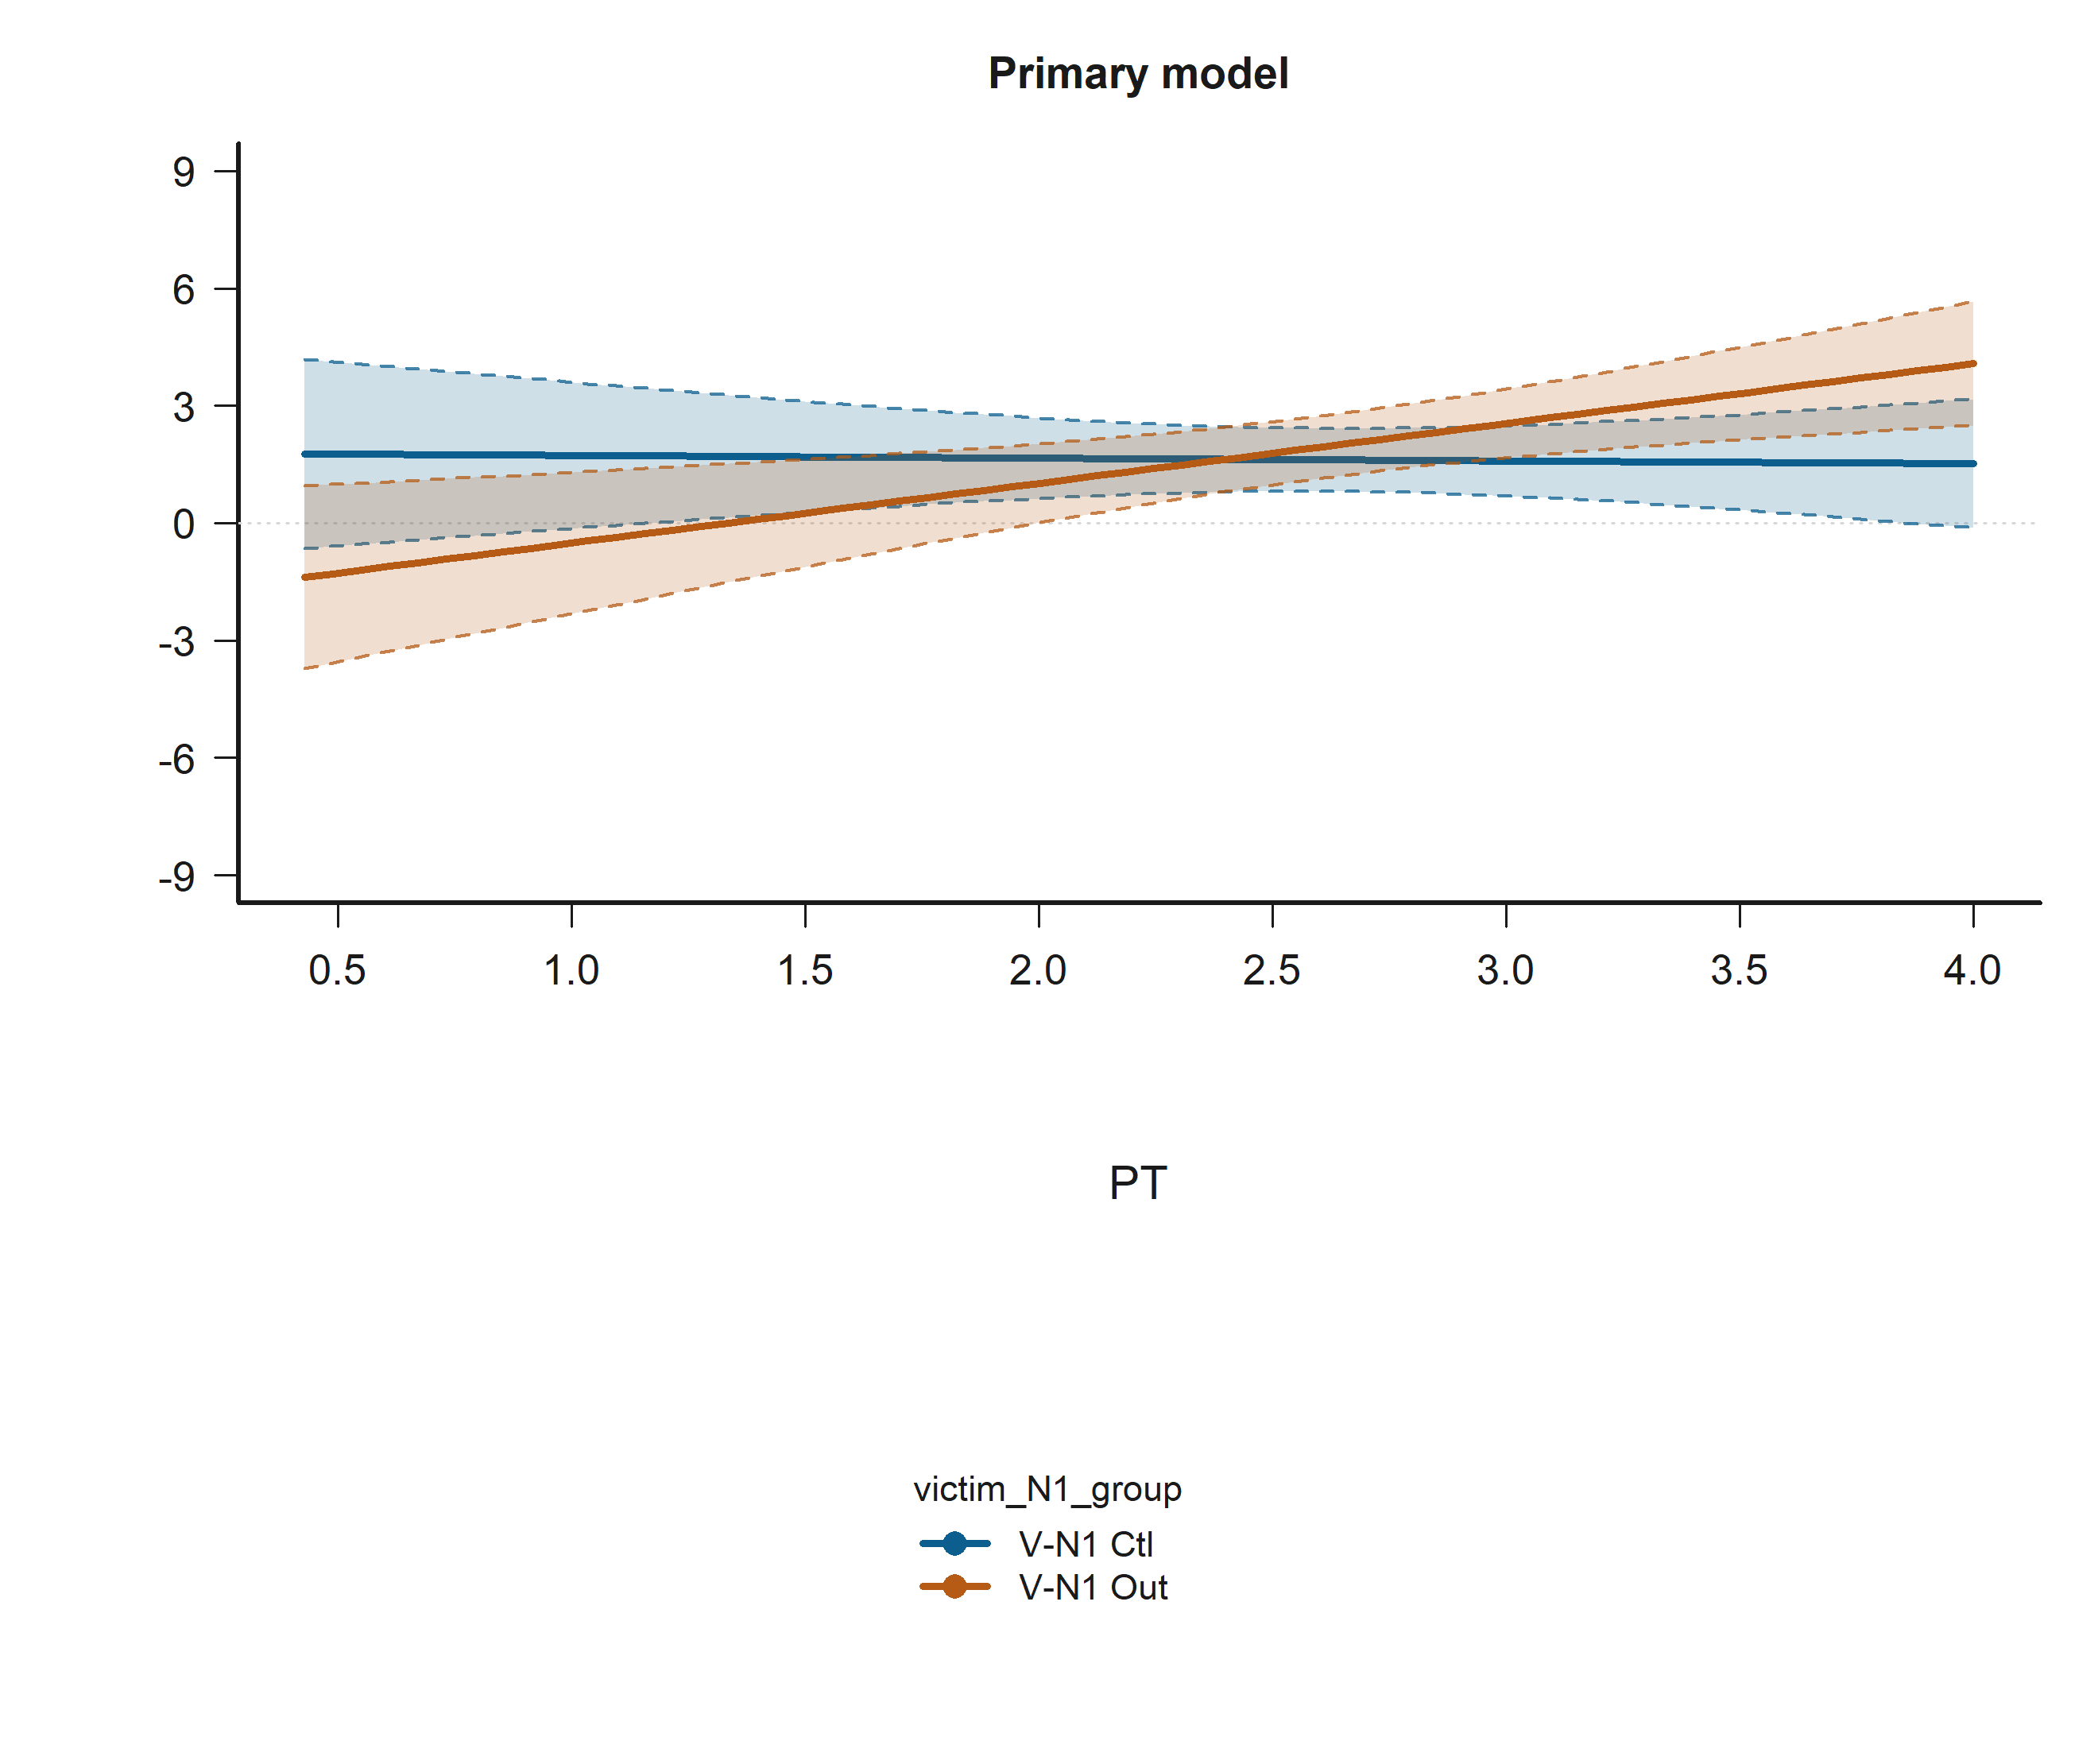
\includegraphics[width=0.92\textwidth]{../figures/figure_sig_H3_iri_pt_victim_n1_groupout_h3_empathy_perspective_taking_x_victim_n1_outgroup_ref_control.png}
\caption{Interaction Plot for Empathy: Perspective taking x Victim-N1: Outgroup (ref = Control) in Empathy x Relational Status. The panels show predicted judgments on the observed -9 to 9 scale with 95\% confidence intervals. Abbrev.: FS / EC / PT / PD = IRI subscales; N1 / N2 = negotiator 1 / negotiator 2; B-V = bystander-victim relation; V-N1 / V-N2 = victim-negotiator relations; B-N1 / B-N2 = bystander-negotiator relations; Vic / Obs = victim / observer subset; In / Out / Ctl = ingroup / outgroup / control label hidden; SameFac = N1 and N2 same faculty; SES = economic status.}
\label{fig:sig_H3_iri_pt_victim_n1_groupout}
\end{figure}

Empathy: Empathic concern x Victim-N1: Outgroup (ref = Control) is statistically significant in the Tobit random-intercepts model (*, p = 0.036). Figure \ref{fig:sig_H3_iri_ec_victim_n1_groupout} shows that the predicted relationship falls most sharply for Empathy: Empathic concern when the condition is V-N1 Out.

\begin{figure}[H]
\centering
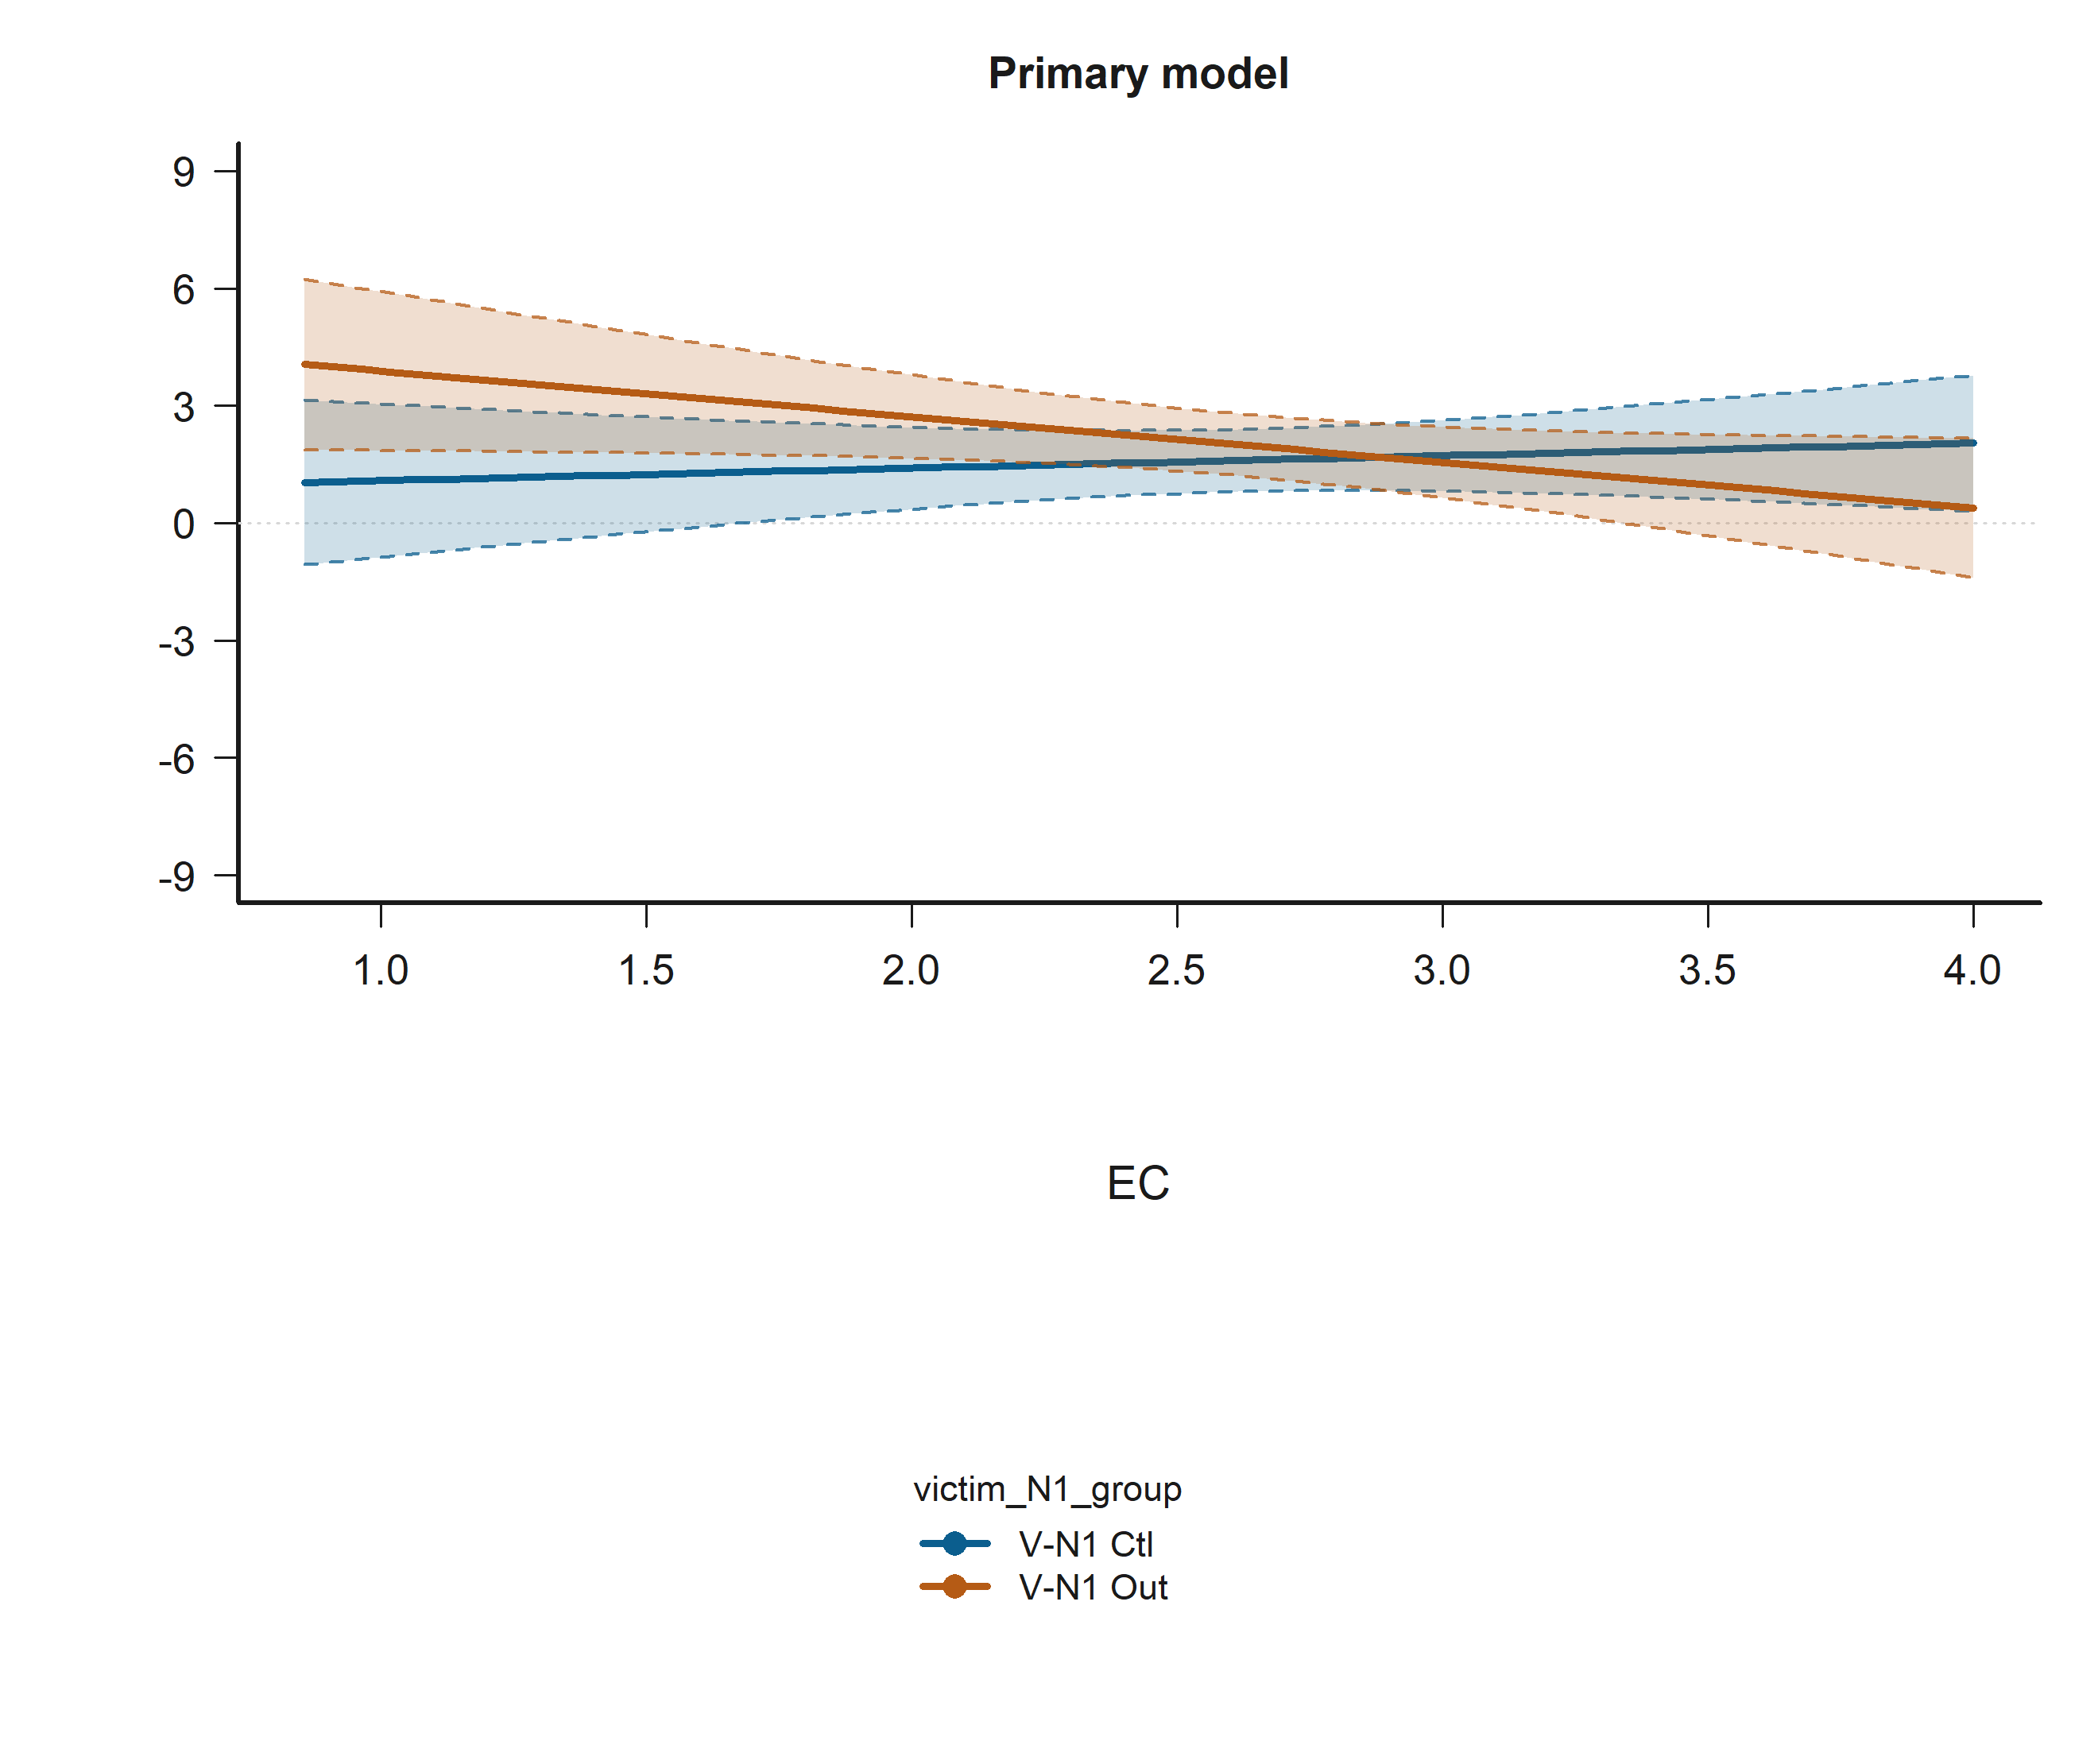
\includegraphics[width=0.92\textwidth]{../figures/figure_sig_H3_iri_ec_victim_n1_groupout_h3_empathy_empathic_concern_x_victim_n1_outgroup_ref_control.png}
\caption{Interaction Plot for Empathy: Empathic concern x Victim-N1: Outgroup (ref = Control) in Empathy x Relational Status. The panels show predicted judgments on the observed -9 to 9 scale with 95\% confidence intervals. Abbrev.: FS / EC / PT / PD = IRI subscales; N1 / N2 = negotiator 1 / negotiator 2; B-V = bystander-victim relation; V-N1 / V-N2 = victim-negotiator relations; B-N1 / B-N2 = bystander-negotiator relations; Vic / Obs = victim / observer subset; In / Out / Ctl = ingroup / outgroup / control label hidden; SameFac = N1 and N2 same faculty; SES = economic status.}
\label{fig:sig_H3_iri_ec_victim_n1_groupout}
\end{figure}

Bystander-N1: Outgroup (ref = Control) x Empathy: Fantasy scale is statistically significant in the Tobit random-intercepts model (*, p = 0.039). Figure \ref{fig:sig_H3_bystander_n1_groupout_iri_fs} shows that the predicted relationship falls most sharply for Empathy: Fantasy scale when the condition is B-N1 Out.

\begin{figure}[H]
\centering
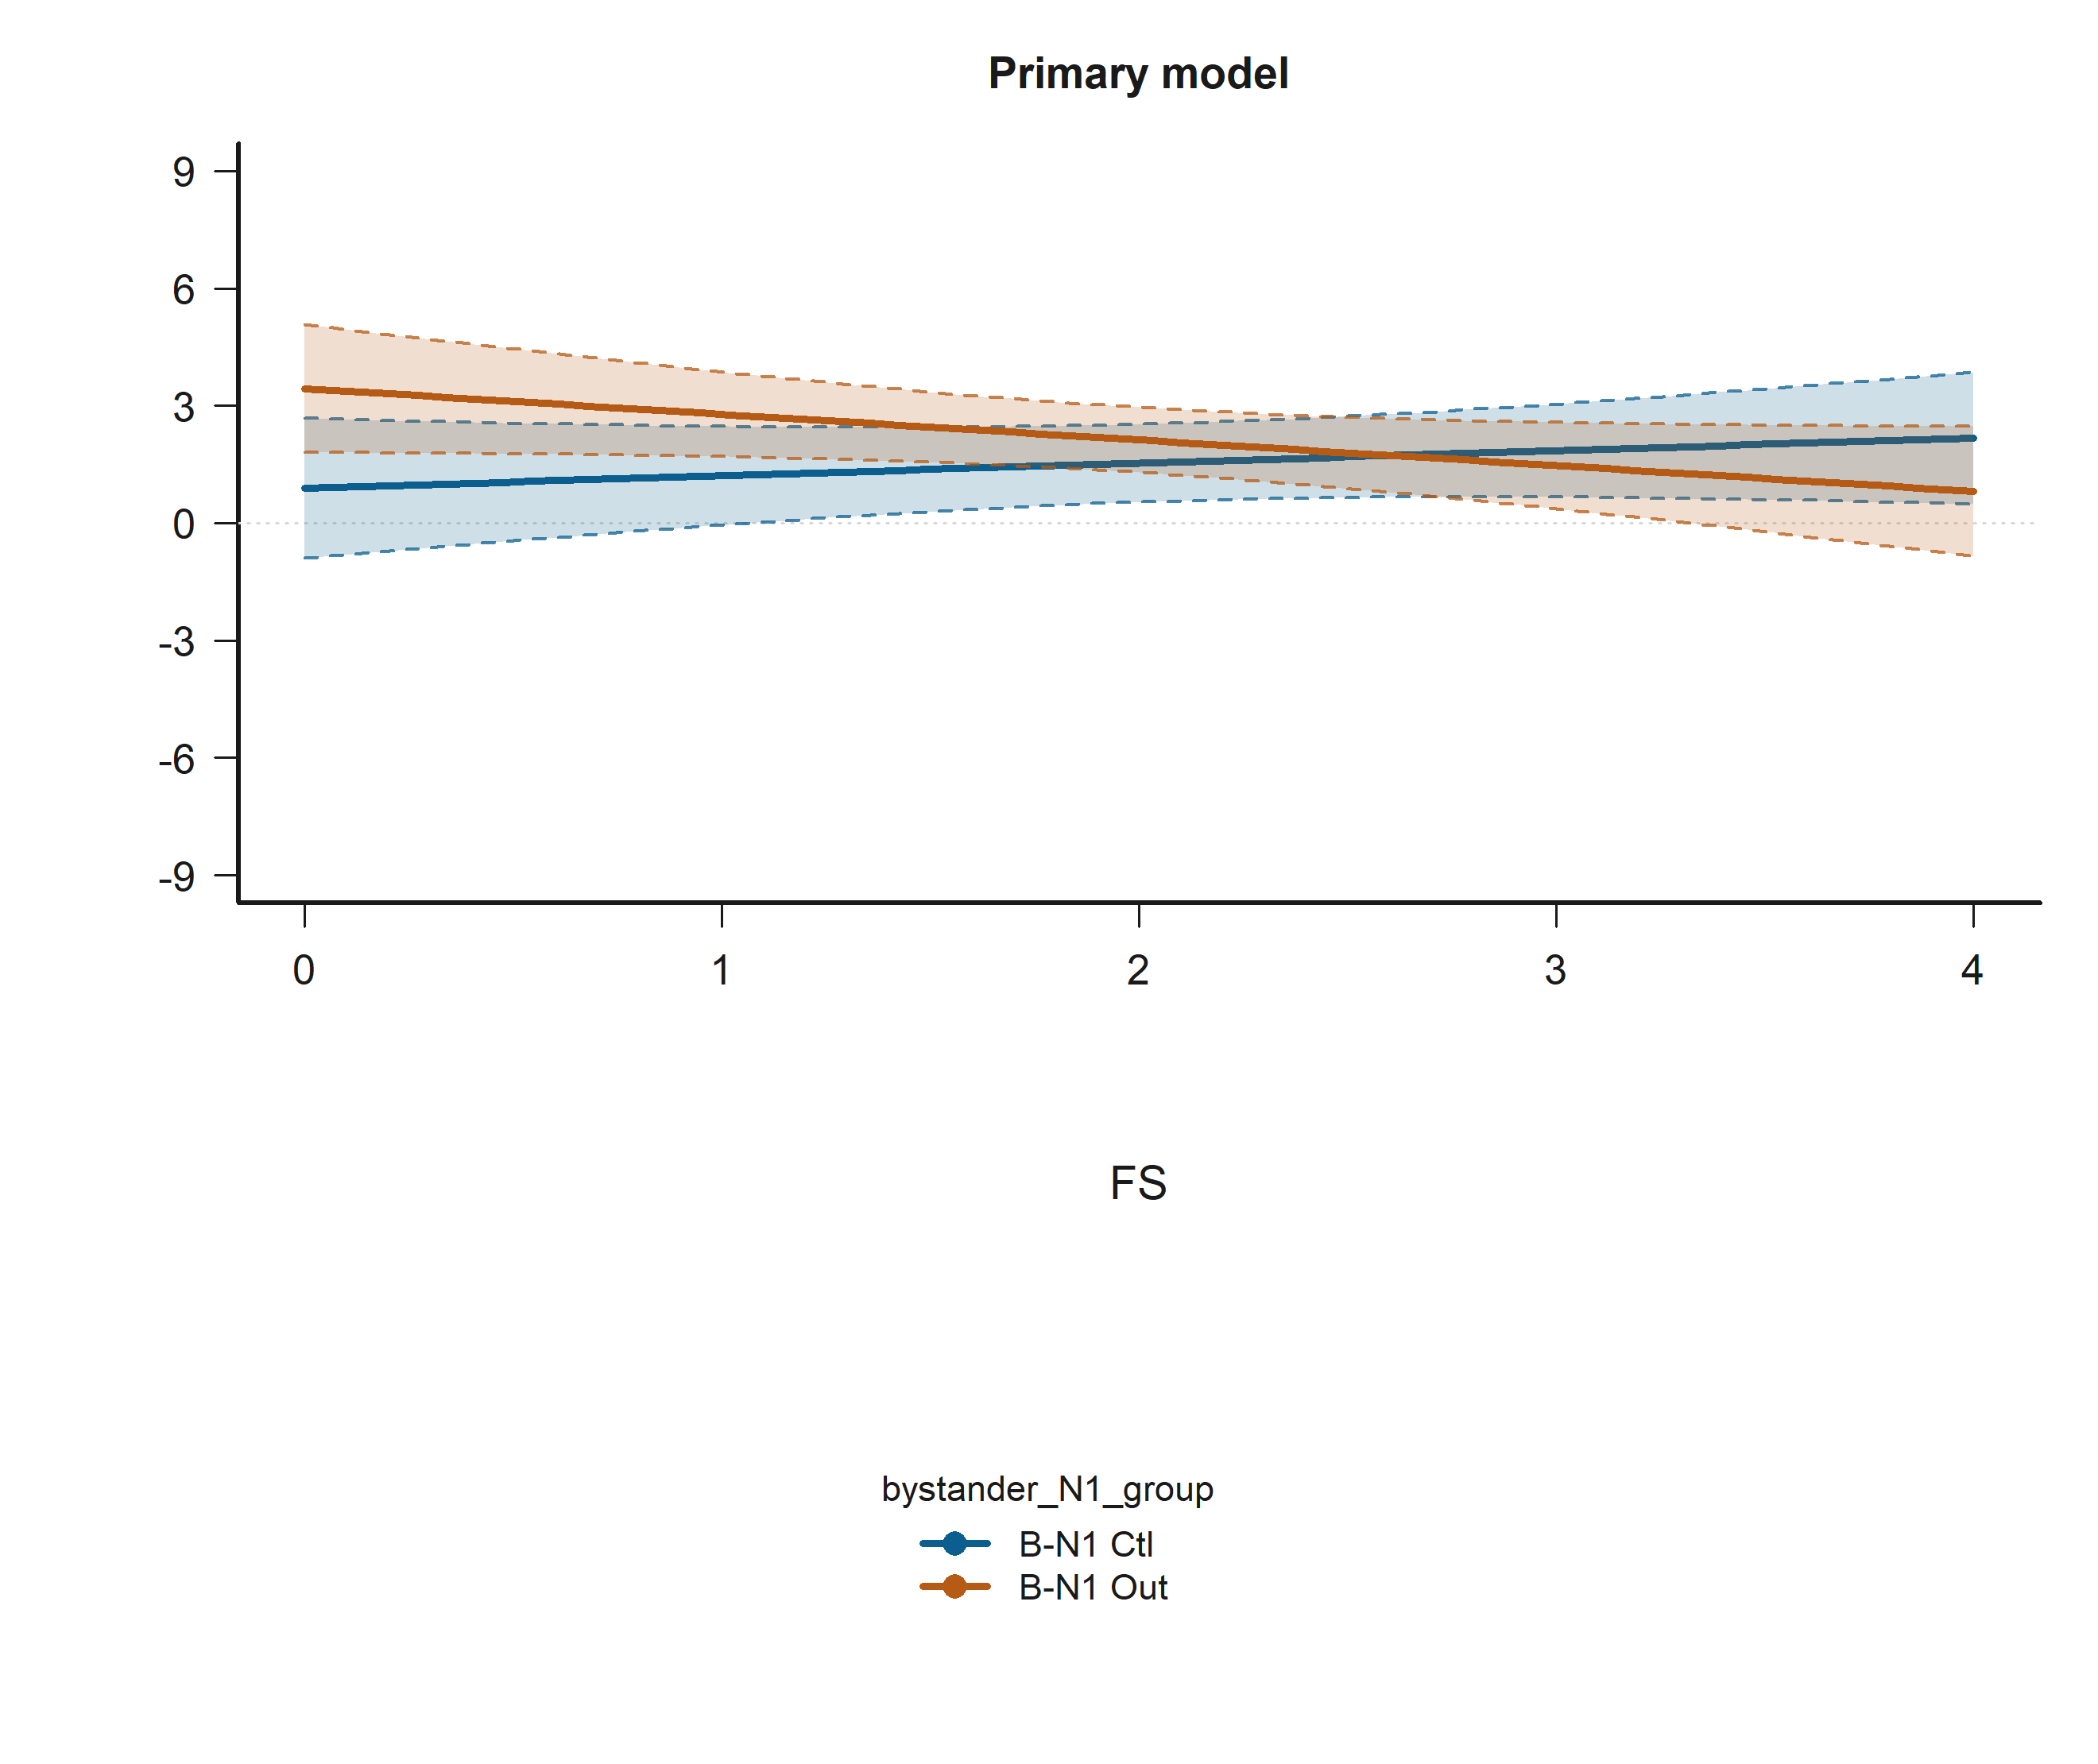
\includegraphics[width=0.92\textwidth]{../figures/figure_sig_H3_bystander_n1_groupout_iri_fs_h3_bystander_n1_outgroup_ref_control_x_empathy_fantasy_scale.png}
\caption{Interaction Plot for Bystander-N1: Outgroup (ref = Control) x Empathy: Fantasy scale in Empathy x Relational Status. The panels show predicted judgments on the observed -9 to 9 scale with 95\% confidence intervals. Abbrev.: FS / EC / PT / PD = IRI subscales; N1 / N2 = negotiator 1 / negotiator 2; B-V = bystander-victim relation; V-N1 / V-N2 = victim-negotiator relations; B-N1 / B-N2 = bystander-negotiator relations; Vic / Obs = victim / observer subset; In / Out / Ctl = ingroup / outgroup / control label hidden; SameFac = N1 and N2 same faculty; SES = economic status.}
\label{fig:sig_H3_bystander_n1_groupout_iri_fs}
\end{figure}

Bystander-victim: Outgroup (ref = Ingroup) x Empathy: Personal distress is statistically significant in the Tobit random-intercepts model (+, p = 0.064). Figure \ref{fig:sig_H3_bystander_victim_groupout_iri_pd} shows that the predicted relationship rises most sharply for Empathy: Personal distress when the condition is B-V Out.

\begin{figure}[H]
\centering
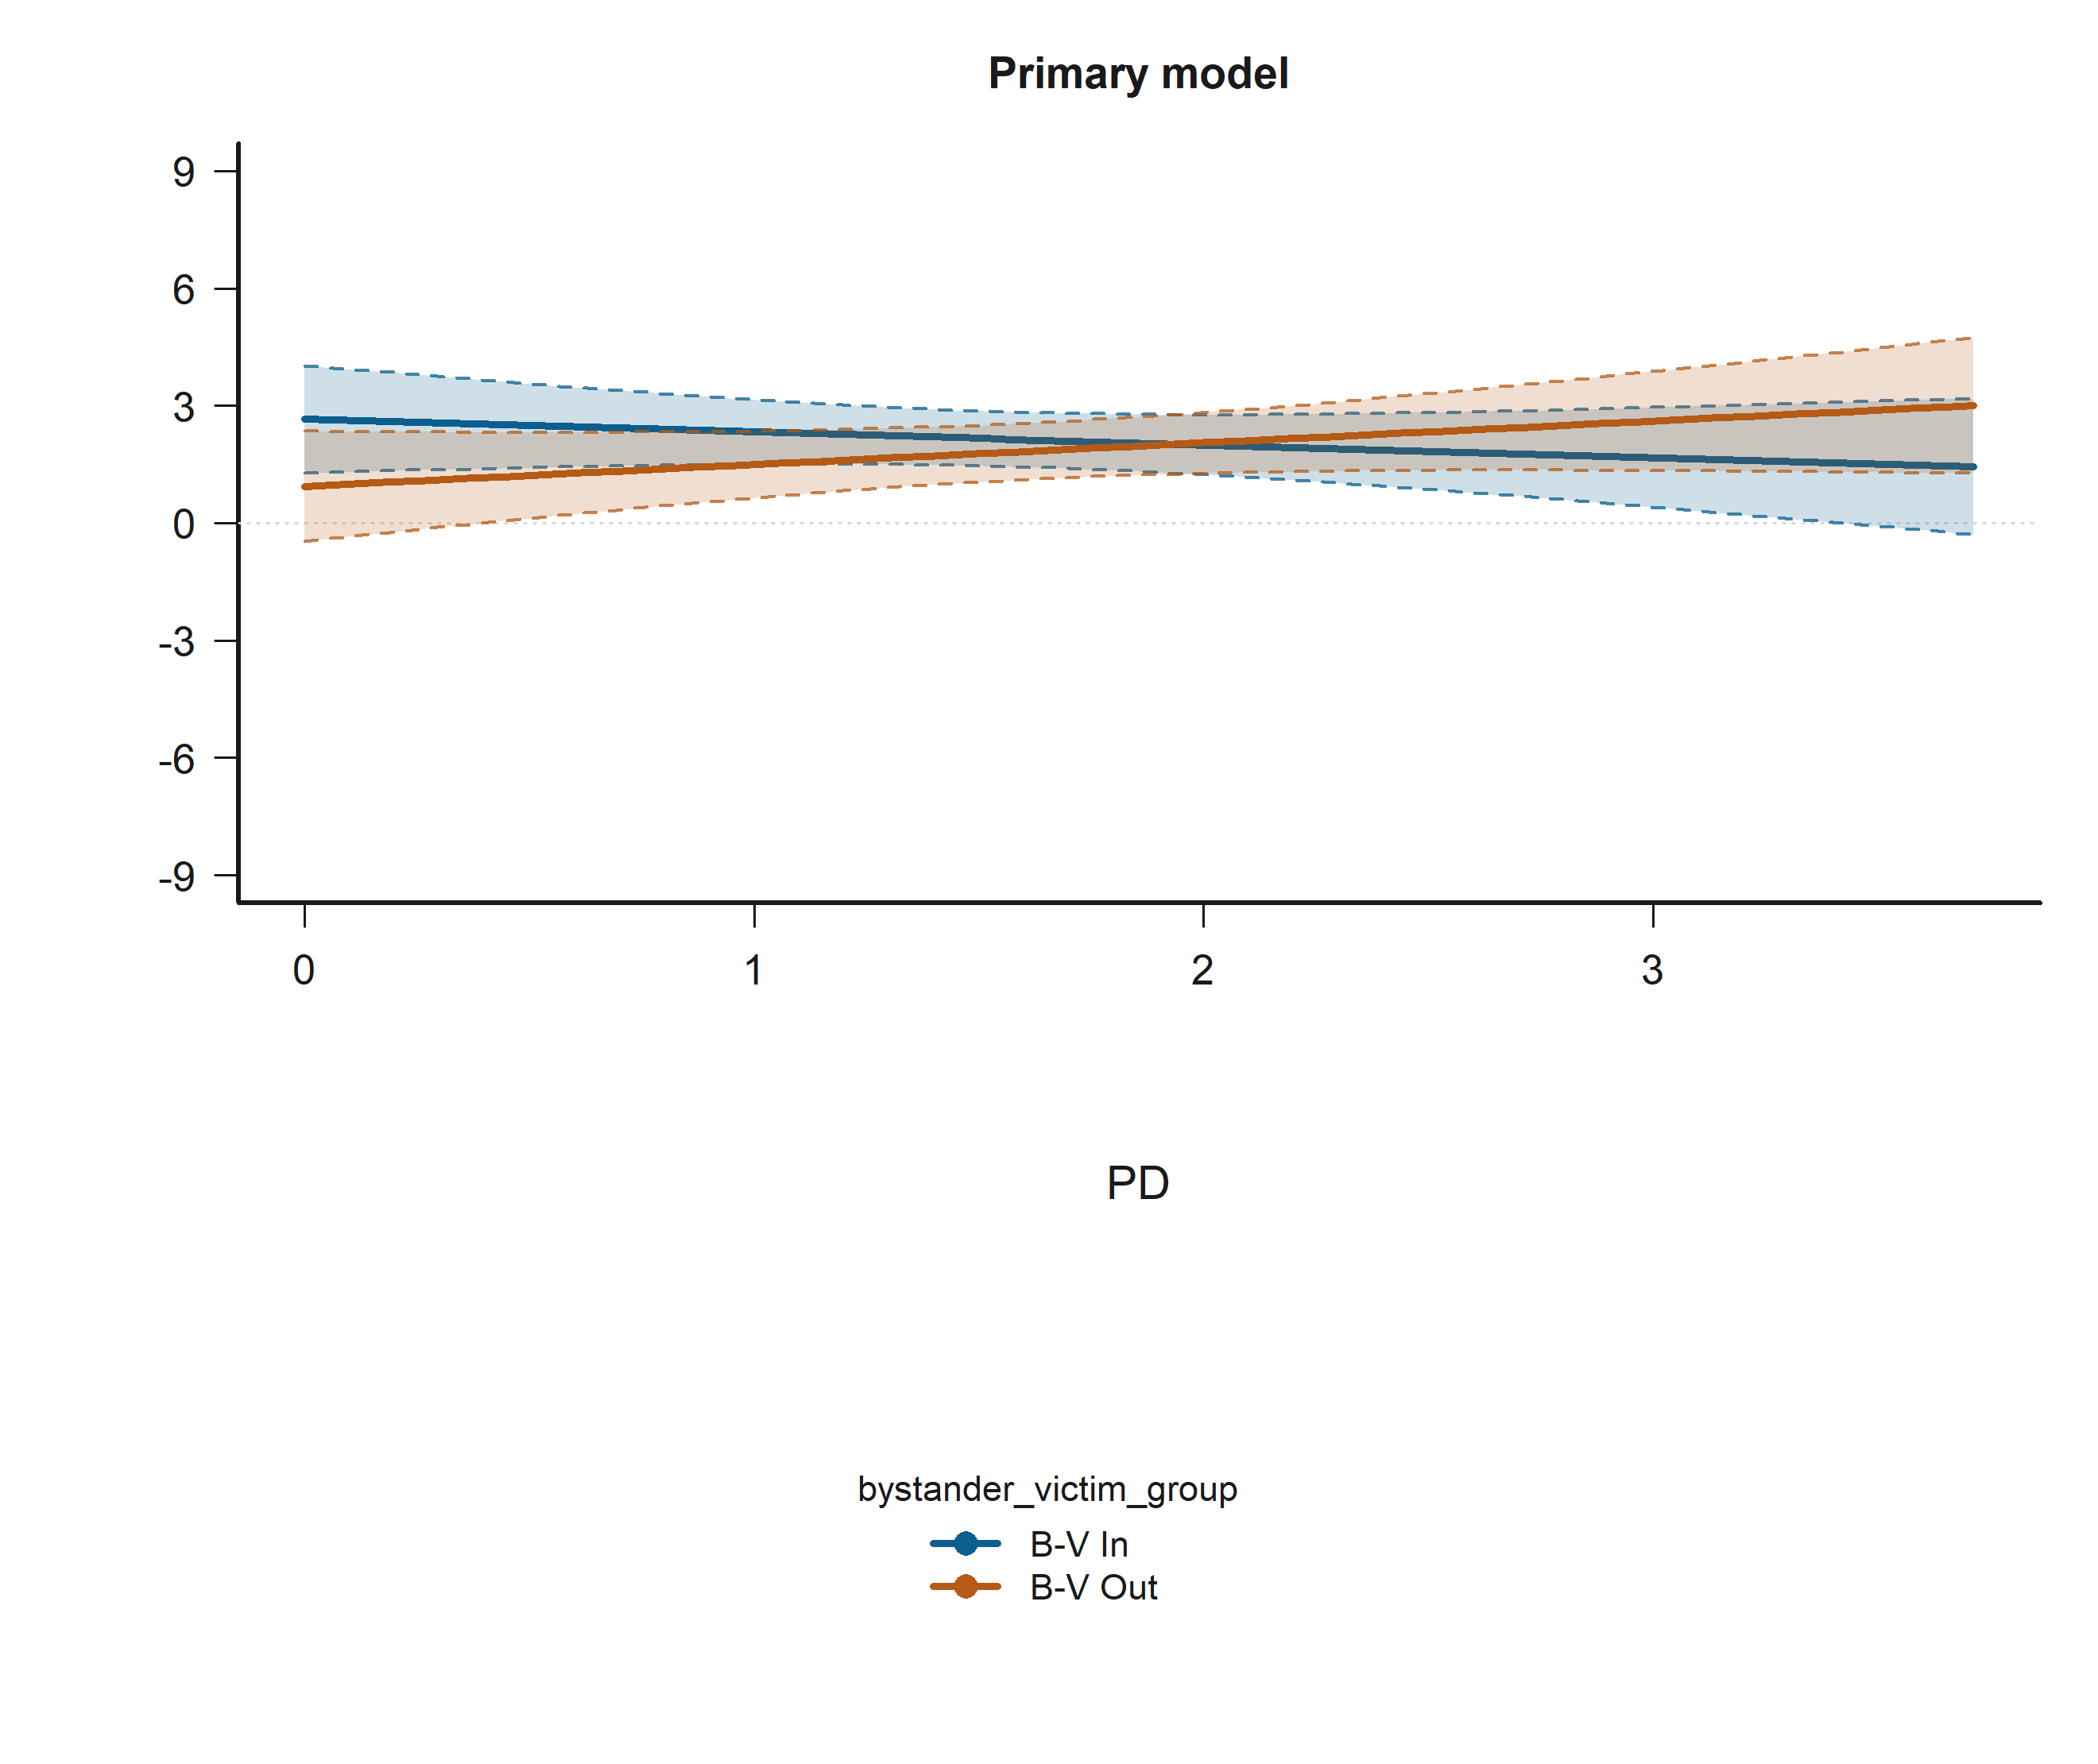
\includegraphics[width=0.92\textwidth]{../figures/figure_sig_H3_bystander_victim_groupout_iri_pd_h3_bystander_victim_outgroup_ref_ingroup_x_empathy_personal_distress.png}
\caption{Interaction Plot for Bystander-victim: Outgroup (ref = Ingroup) x Empathy: Personal distress in Empathy x Relational Status. The panels show predicted judgments on the observed -9 to 9 scale with 95\% confidence intervals. Abbrev.: FS / EC / PT / PD = IRI subscales; N1 / N2 = negotiator 1 / negotiator 2; B-V = bystander-victim relation; V-N1 / V-N2 = victim-negotiator relations; B-N1 / B-N2 = bystander-negotiator relations; Vic / Obs = victim / observer subset; In / Out / Ctl = ingroup / outgroup / control label hidden; SameFac = N1 and N2 same faculty; SES = economic status.}
\label{fig:sig_H3_bystander_victim_groupout_iri_pd}
\end{figure}

Bystander-N2: Outgroup (ref = Control) x Empathy: Perspective taking is statistically significant in the Tobit random-intercepts model (+, p = 0.084). Figure \ref{fig:sig_H3_bystander_n2_groupout_iri_pt} shows that the predicted relationship rises most sharply for Empathy: Perspective taking when the condition is B-N2 Ctl.

\begin{figure}[H]
\centering
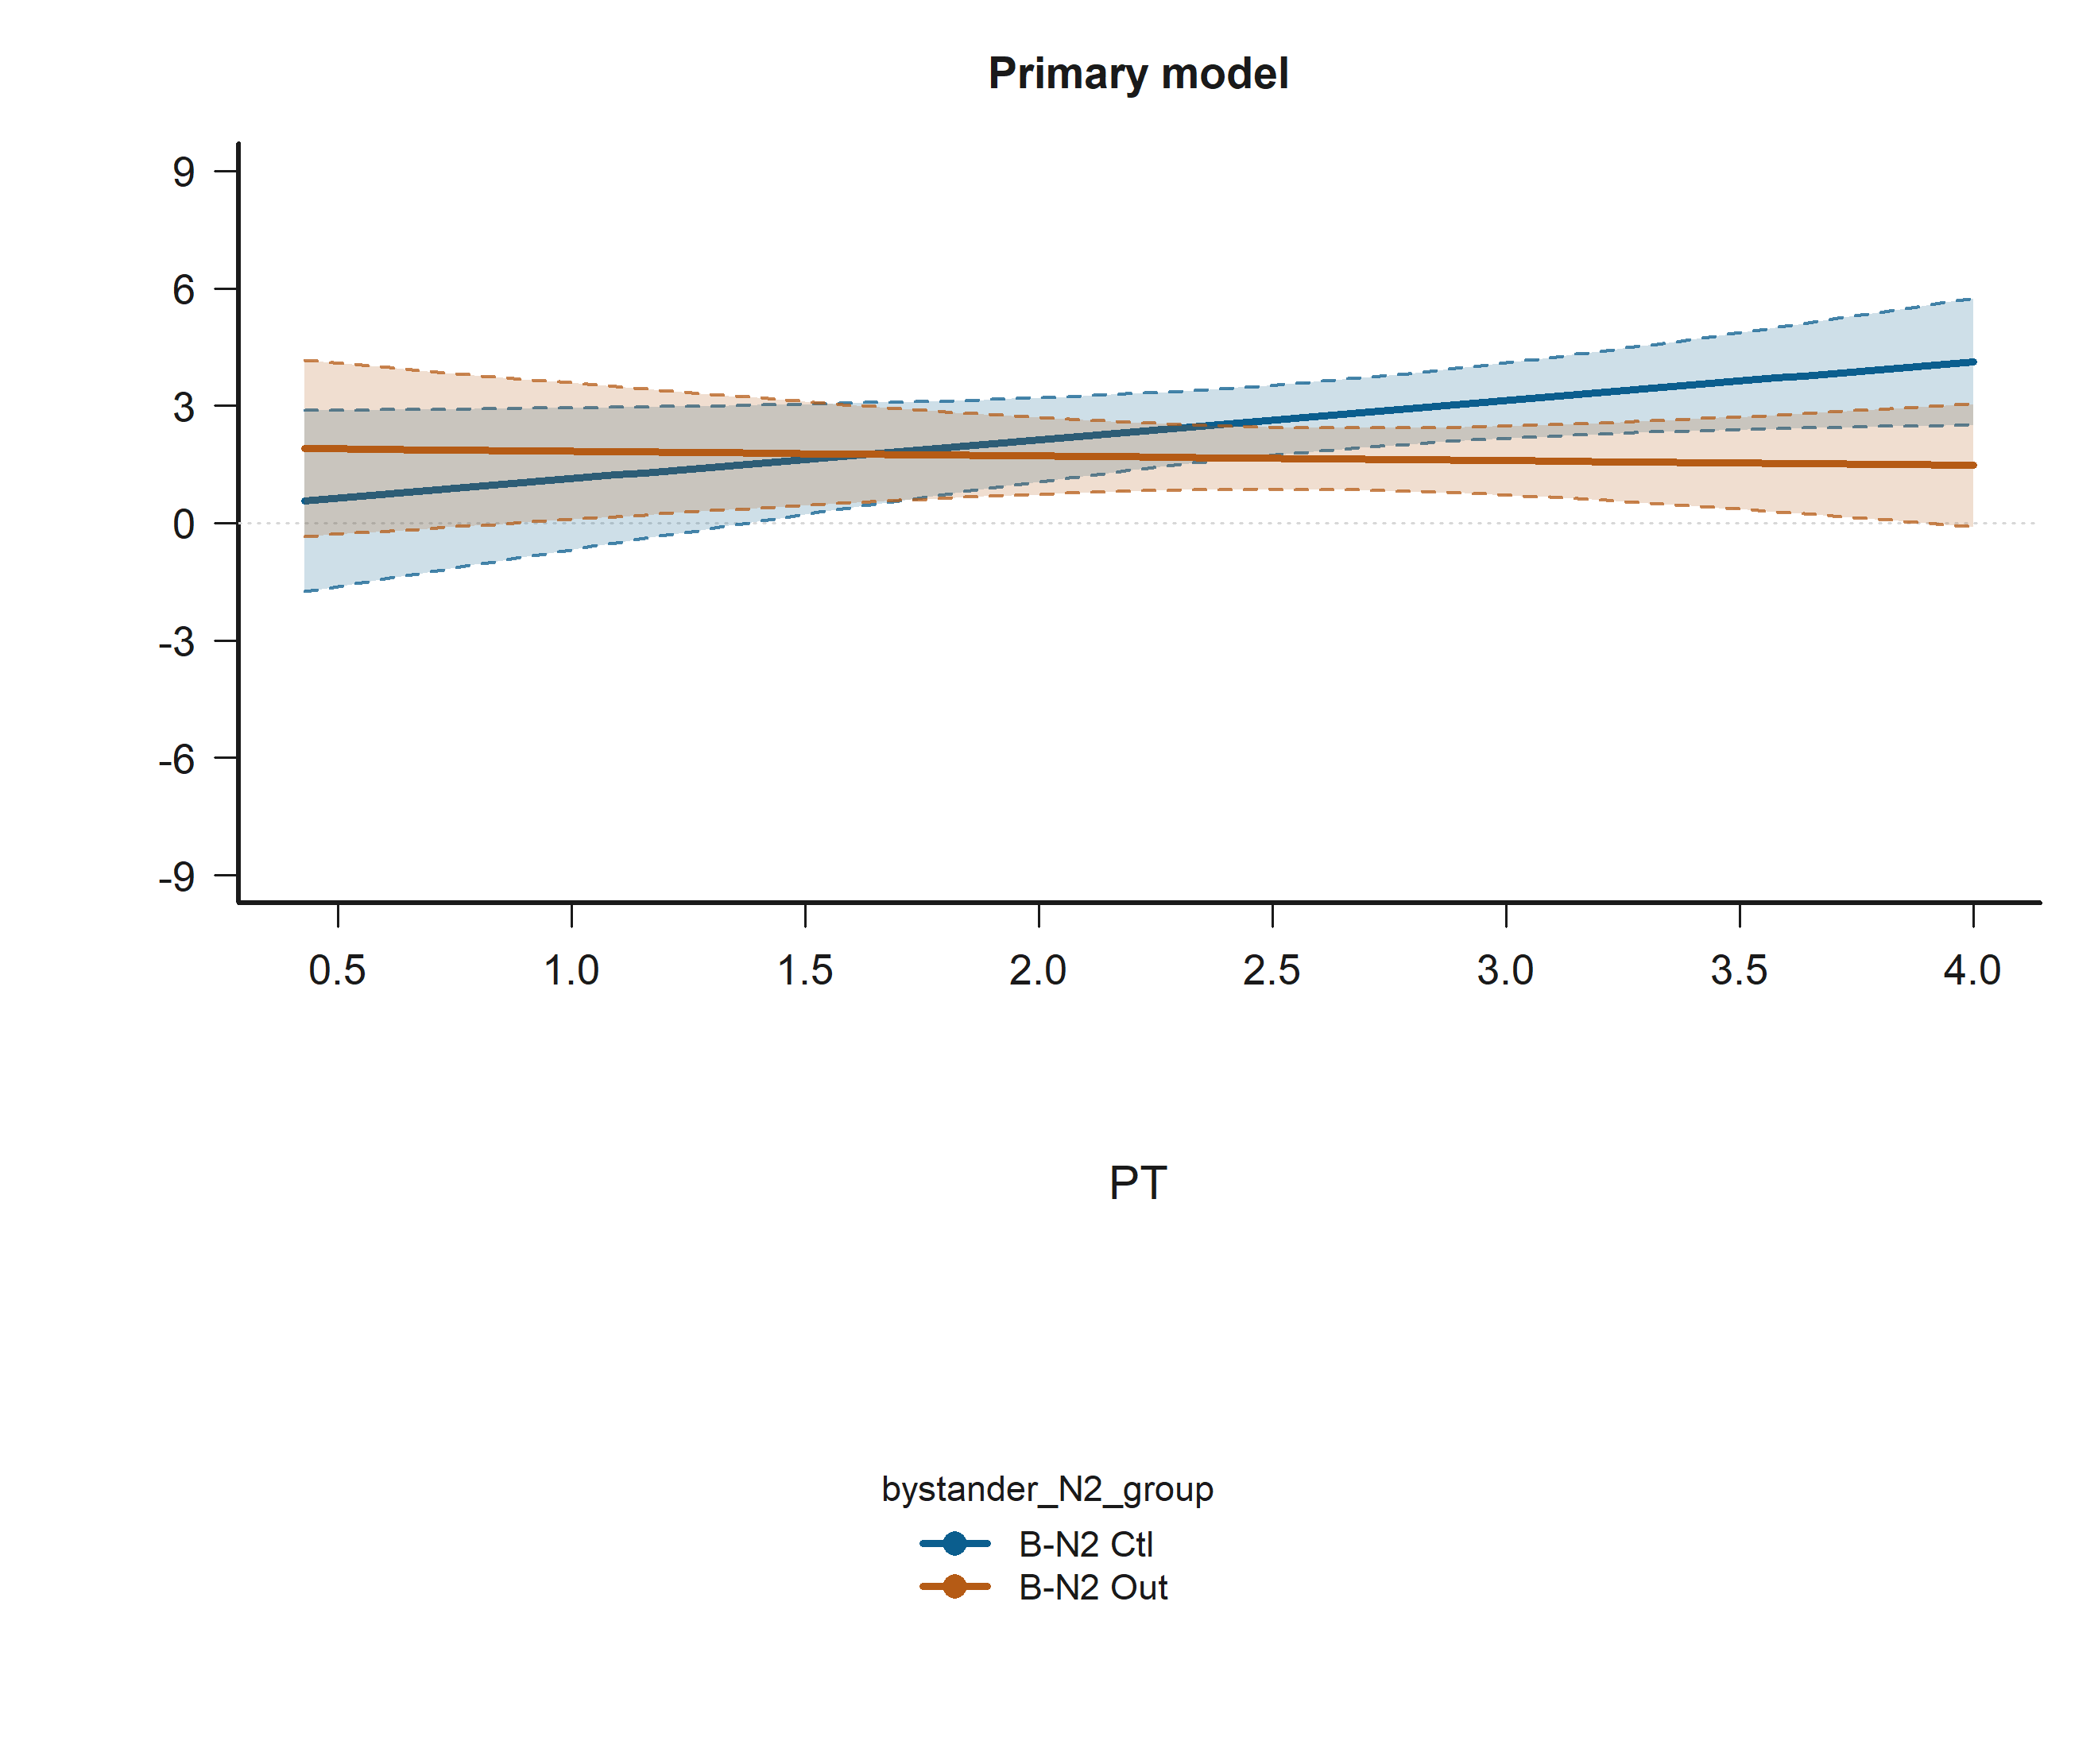
\includegraphics[width=0.92\textwidth]{../figures/figure_sig_H3_bystander_n2_groupout_iri_pt_h3_bystander_n2_outgroup_ref_control_x_empathy_perspective_taking.png}
\caption{Interaction Plot for Bystander-N2: Outgroup (ref = Control) x Empathy: Perspective taking in Empathy x Relational Status. The panels show predicted judgments on the observed -9 to 9 scale with 95\% confidence intervals. Abbrev.: FS / EC / PT / PD = IRI subscales; N1 / N2 = negotiator 1 / negotiator 2; B-V = bystander-victim relation; V-N1 / V-N2 = victim-negotiator relations; B-N1 / B-N2 = bystander-negotiator relations; Vic / Obs = victim / observer subset; In / Out / Ctl = ingroup / outgroup / control label hidden; SameFac = N1 and N2 same faculty; SES = economic status.}
\label{fig:sig_H3_bystander_n2_groupout_iri_pt}
\end{figure}


\subsection{All Significant Predictors (p < 0.10)}
The following figures extend beyond the hypothesis-target terms and visualize every predictor that reaches p < 0.10 in the available H1-H3 Tobit random-intercepts models. This includes significant controls such as age when they clear the threshold.

\paragraph{judgments\_bystander}

Age is statistically significant in:
\begin{itemize}
  \item Empathy x Relational Status Model B (Tobit random-intercepts)
  \item Negotiator-Side Structure Model B (Tobit random-intercepts)
  \item Empathy Effect Model B (Tobit random-intercepts)
\end{itemize}
Figure \ref{fig:sig_all_judgments_bystander_age} shows that across the observed range, higher Age corresponds to higher predicted judgment.

\begin{figure}[H]
\centering
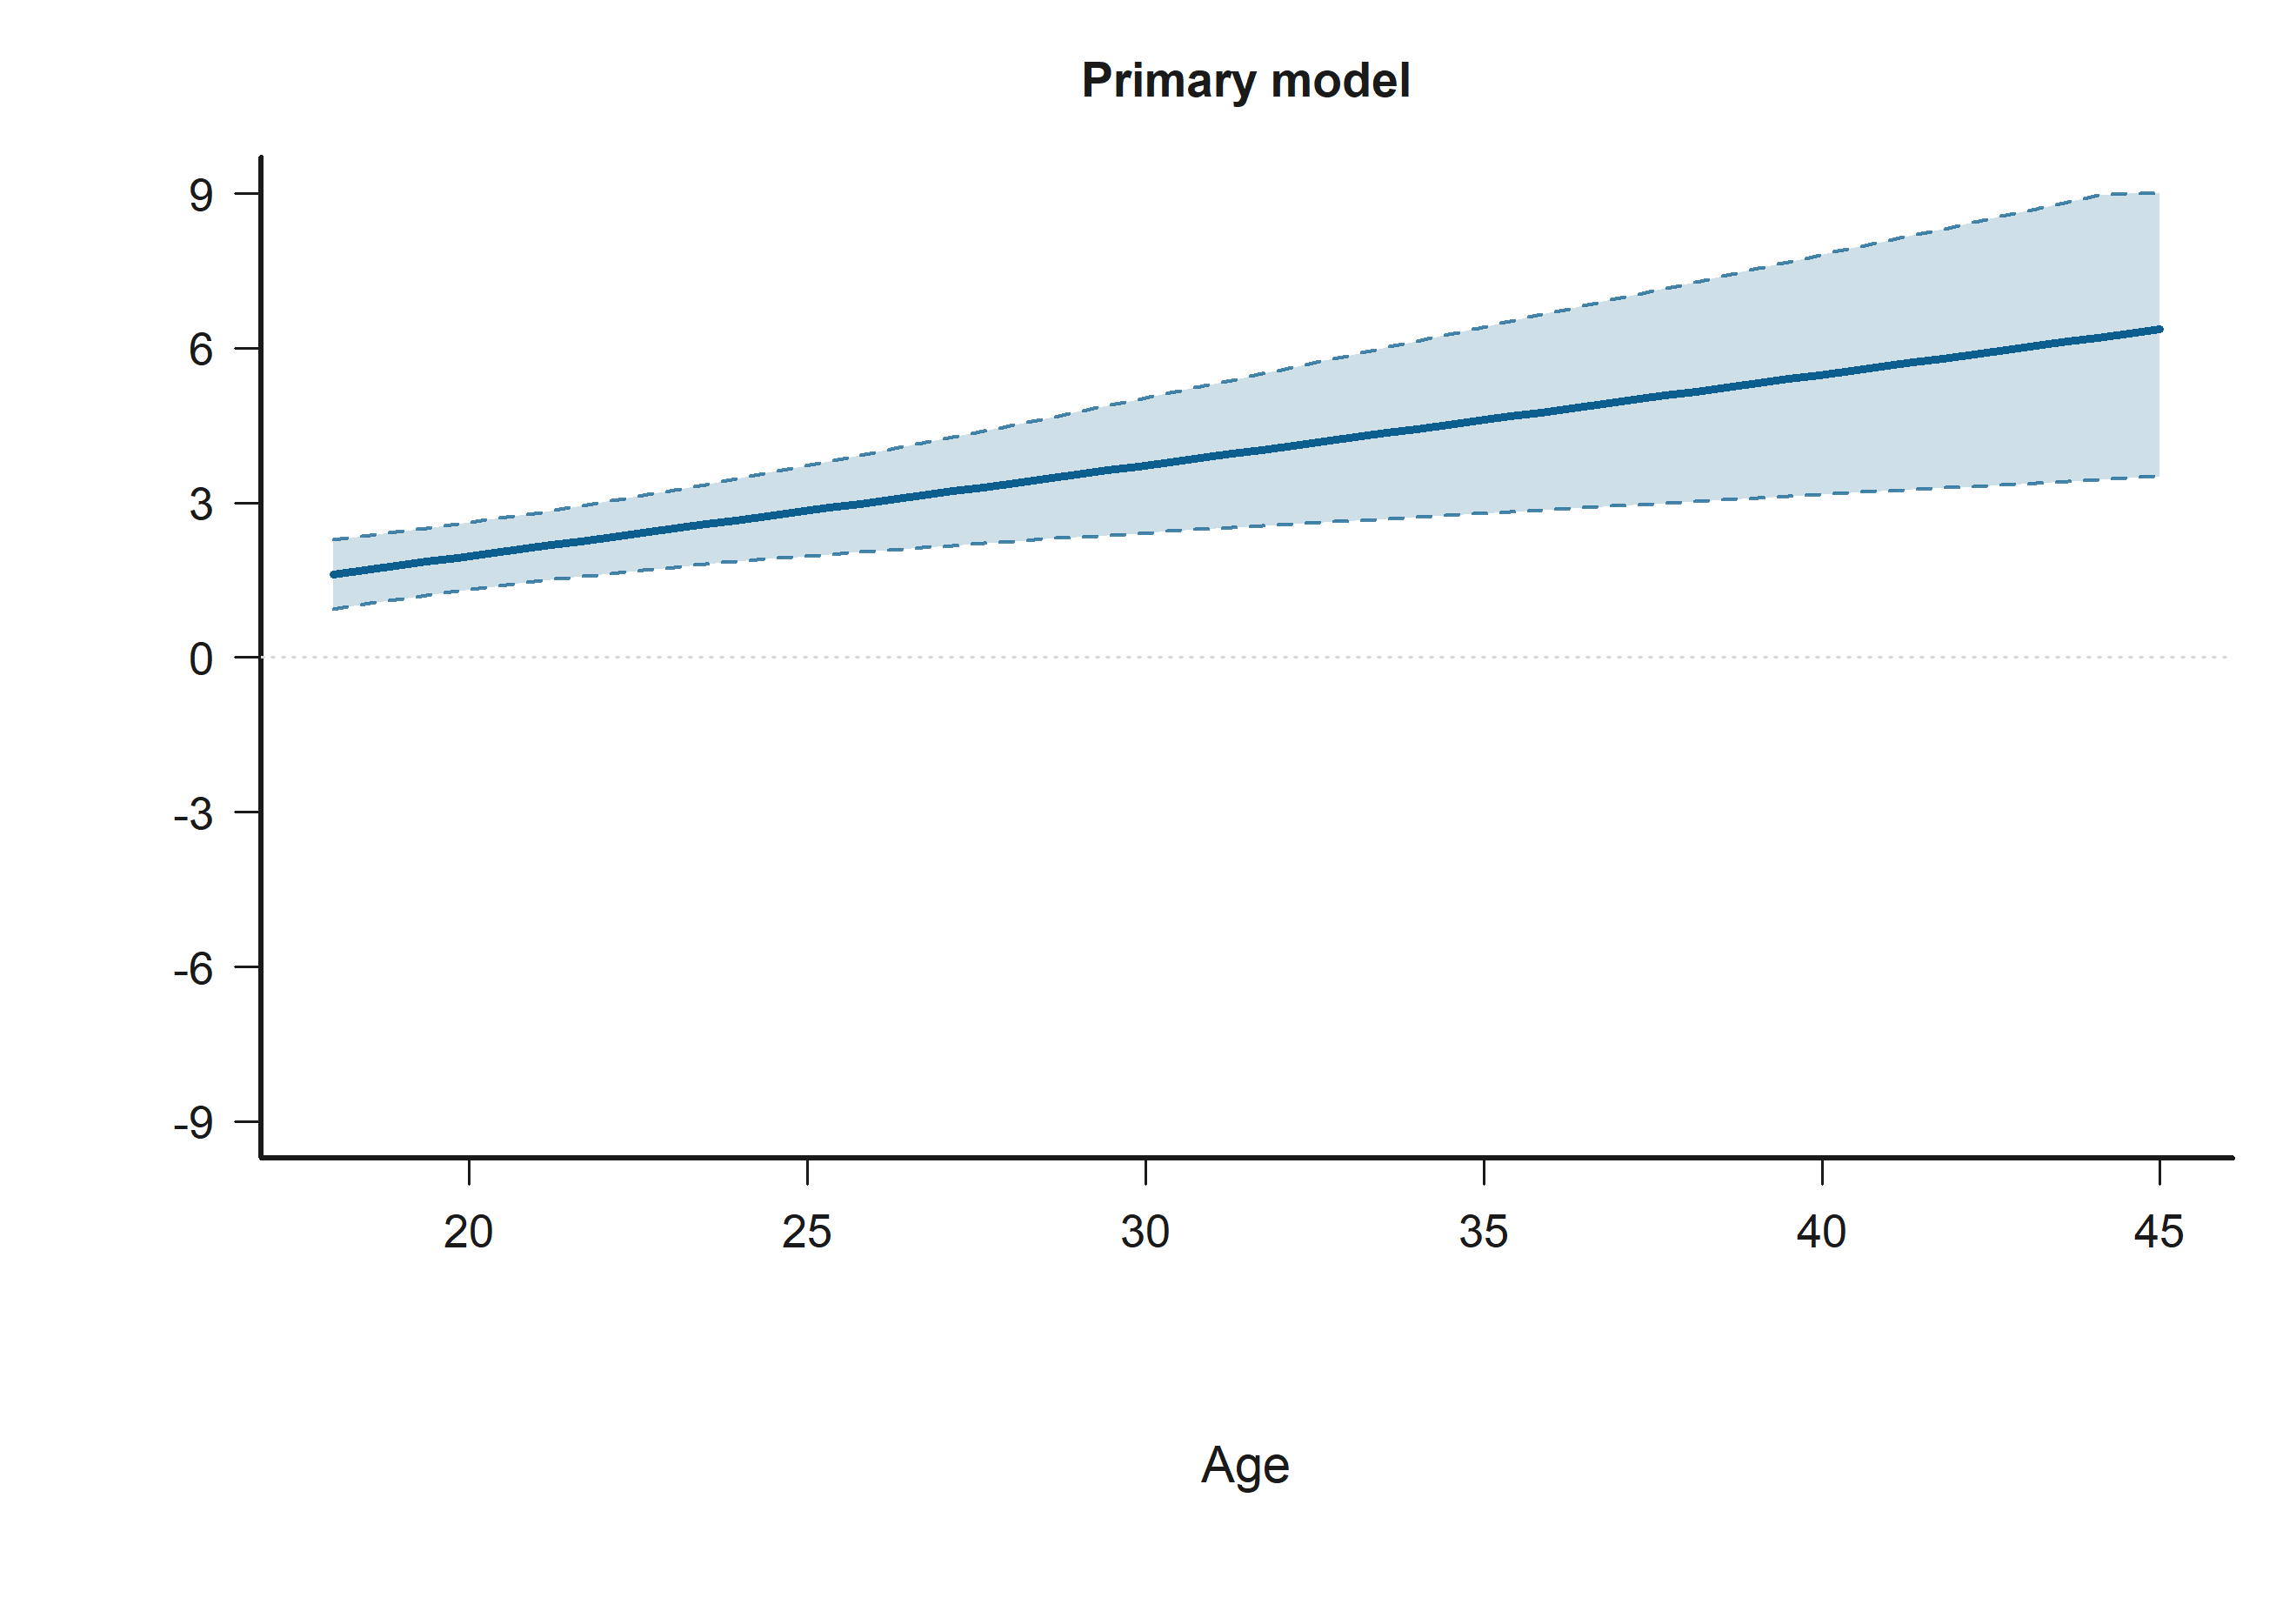
\includegraphics[width=0.92\textwidth]{../figures/figure_sig_all_judgments_bystander_age_judgments_bystander_age.png}
\caption{Effect Plot for Age in the judgments\_bystander. The panels show predicted judgments on the observed -9 to 9 scale with 95\% confidence intervals. Abbrev.: FS / EC / PT / PD = IRI subscales; N1 / N2 = negotiator 1 / negotiator 2; B-V = bystander-victim relation; V-N1 / V-N2 = victim-negotiator relations; B-N1 / B-N2 = bystander-negotiator relations; Vic / Obs = victim / observer subset; In / Out / Ctl = ingroup / outgroup / control label hidden; SameFac = N1 and N2 same faculty; SES = economic status.}
\label{fig:sig_all_judgments_bystander_age}
\end{figure}

Bystander-victim: Outgroup (ref = Ingroup) is statistically significant in:
\begin{itemize}
  \item Negotiator-Side Structure Model B (Tobit random-intercepts)
\end{itemize}
Figure \ref{fig:sig_all_judgments_bystander_bystander_victim_groupout} shows that predicted judgment is lower for B-V Out than for B-V In.

\begin{figure}[H]
\centering
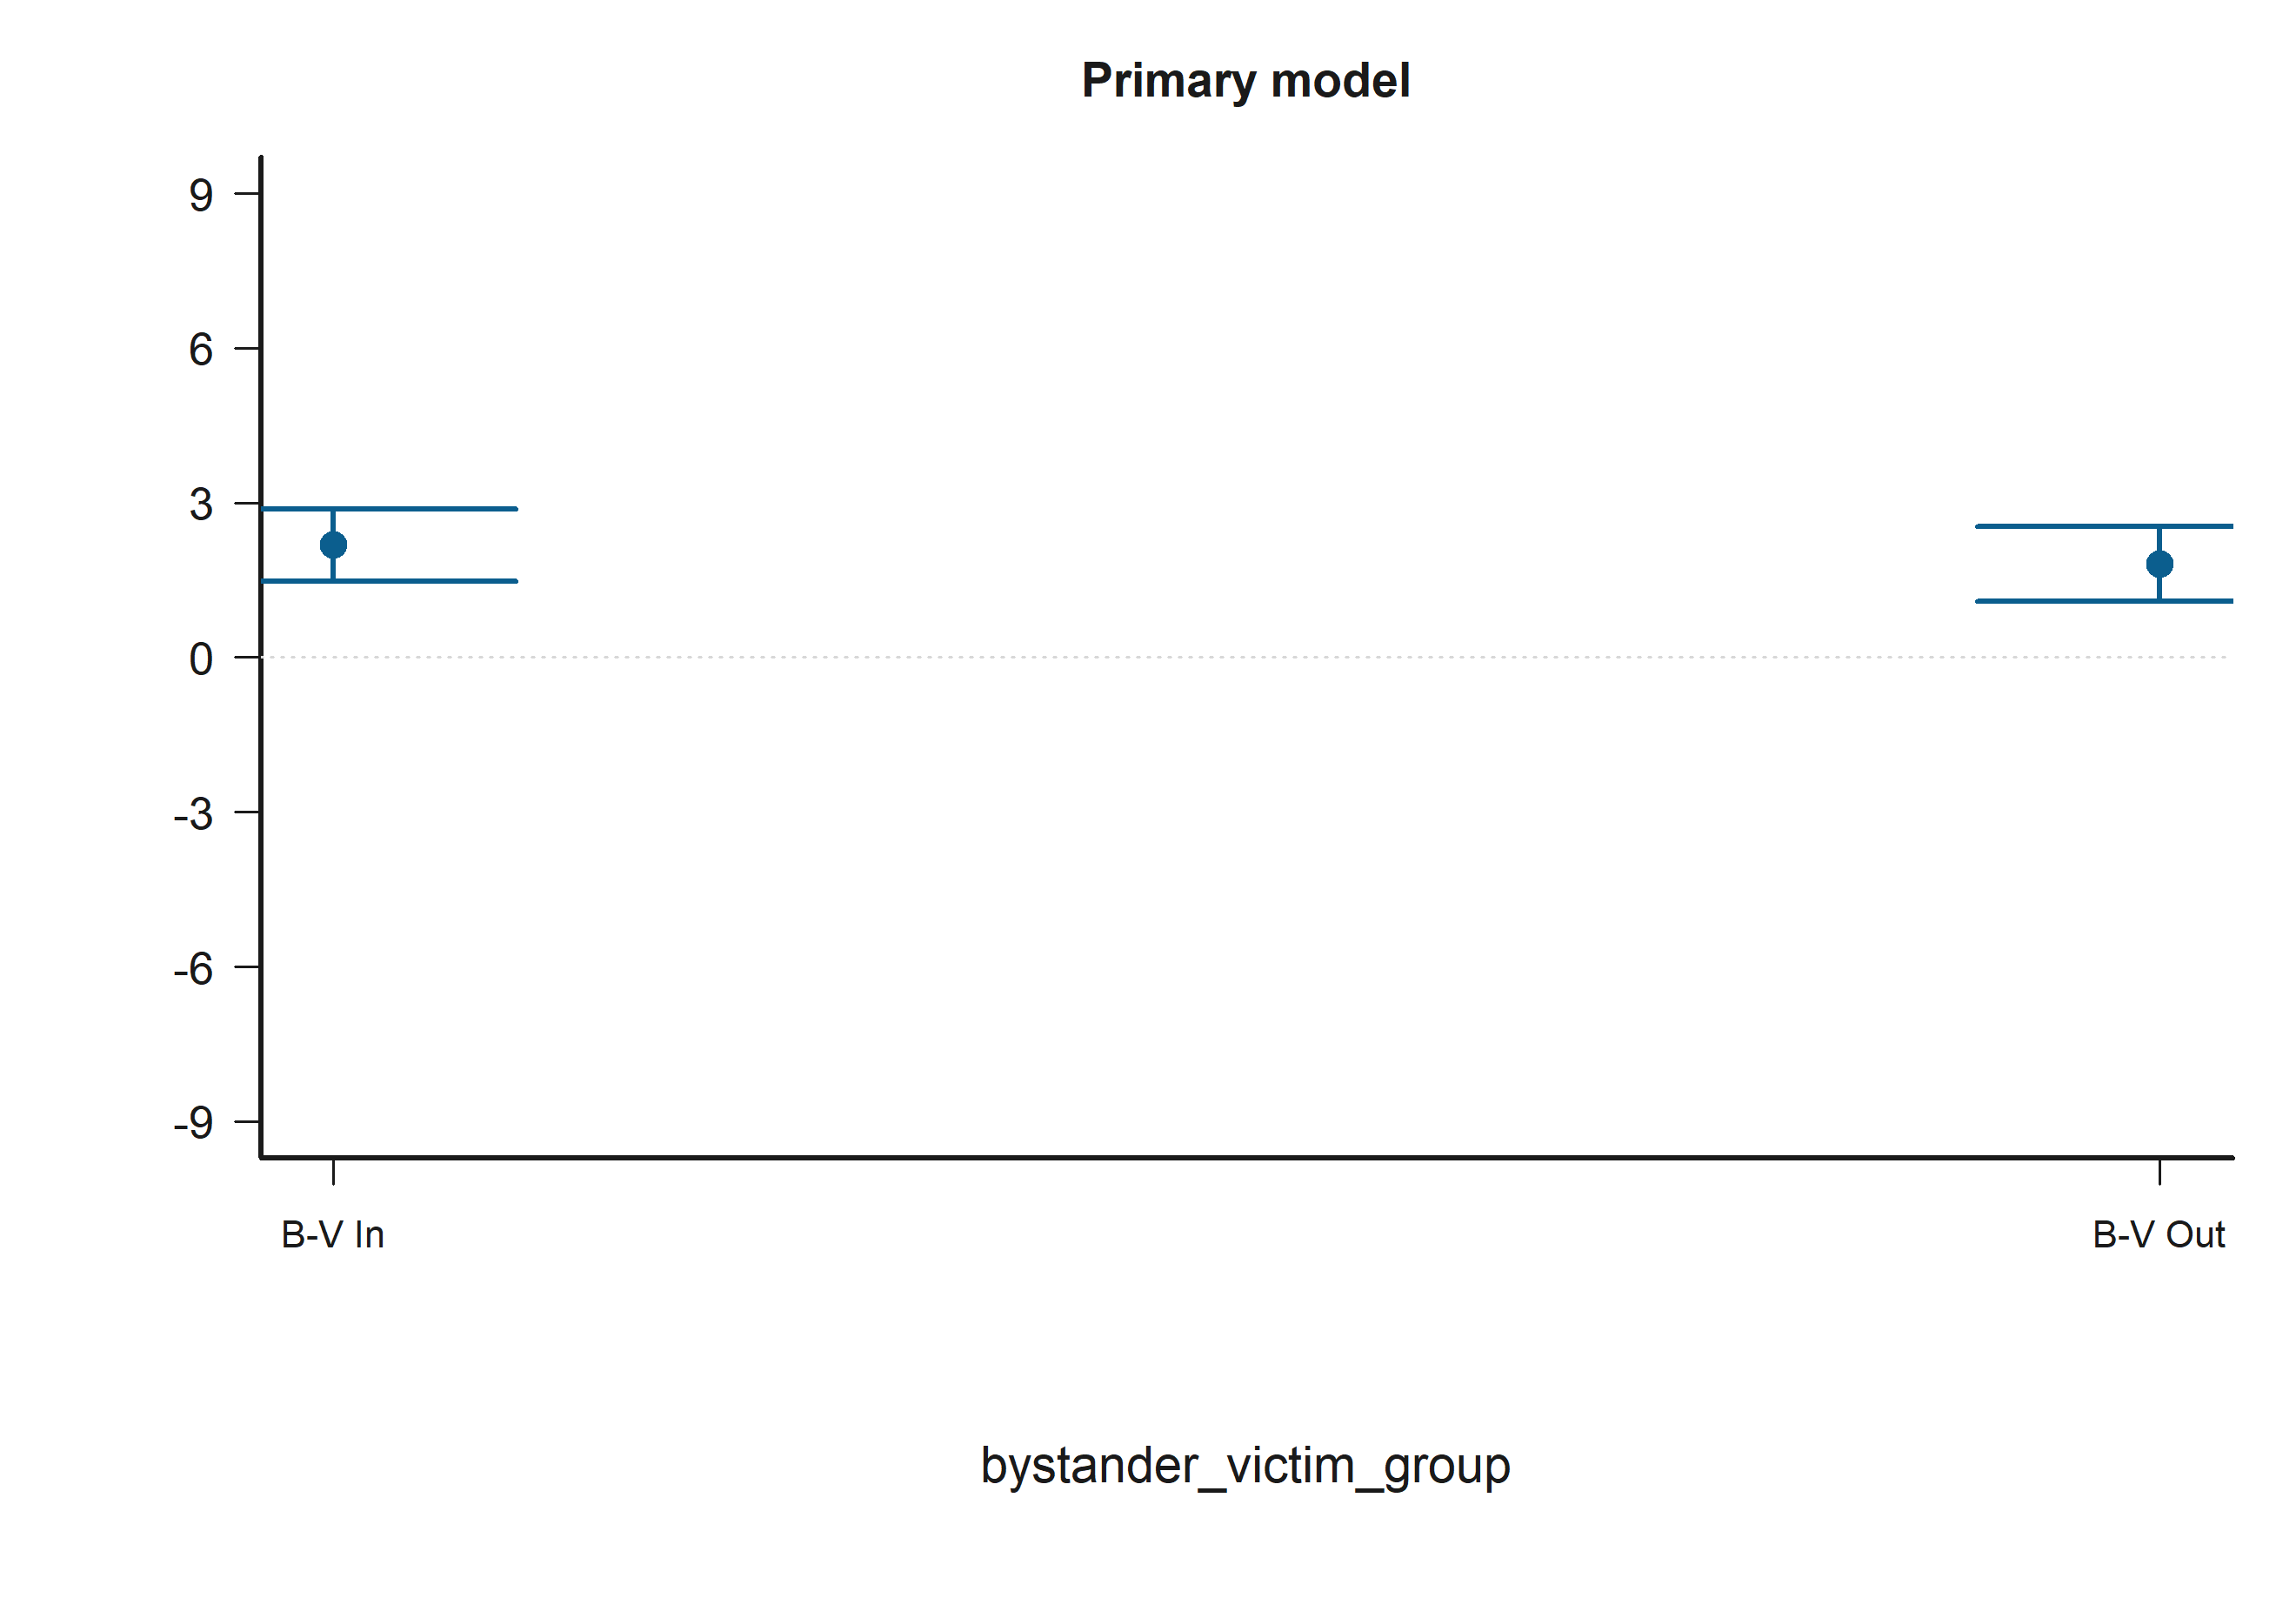
\includegraphics[width=0.92\textwidth]{../figures/figure_sig_all_judgments_bystander_bystander_victim_groupout_judgments_bystander_bystander_victim_outgroup_ref_ingroup.png}
\caption{Grouped Prediction Plot for Bystander-victim: Outgroup (ref = Ingroup) in the judgments\_bystander. The panels show predicted judgments on the observed -9 to 9 scale with 95\% confidence intervals. Abbrev.: FS / EC / PT / PD = IRI subscales; N1 / N2 = negotiator 1 / negotiator 2; B-V = bystander-victim relation; V-N1 / V-N2 = victim-negotiator relations; B-N1 / B-N2 = bystander-negotiator relations; Vic / Obs = victim / observer subset; In / Out / Ctl = ingroup / outgroup / control label hidden; SameFac = N1 and N2 same faculty; SES = economic status.}
\label{fig:sig_all_judgments_bystander_bystander_victim_groupout}
\end{figure}

Bystander-N1: Outgroup (ref = Control) x Empathy: Fantasy scale is statistically significant in:
\begin{itemize}
  \item Empathy x Relational Status Model B (Tobit random-intercepts)
\end{itemize}
Figure \ref{fig:sig_all_judgments_bystander_bystander_n1_groupout_iri_fs} shows that the predicted relationship falls most sharply for Empathy: Fantasy scale when the condition is B-N1 Out.

\begin{figure}[H]
\centering
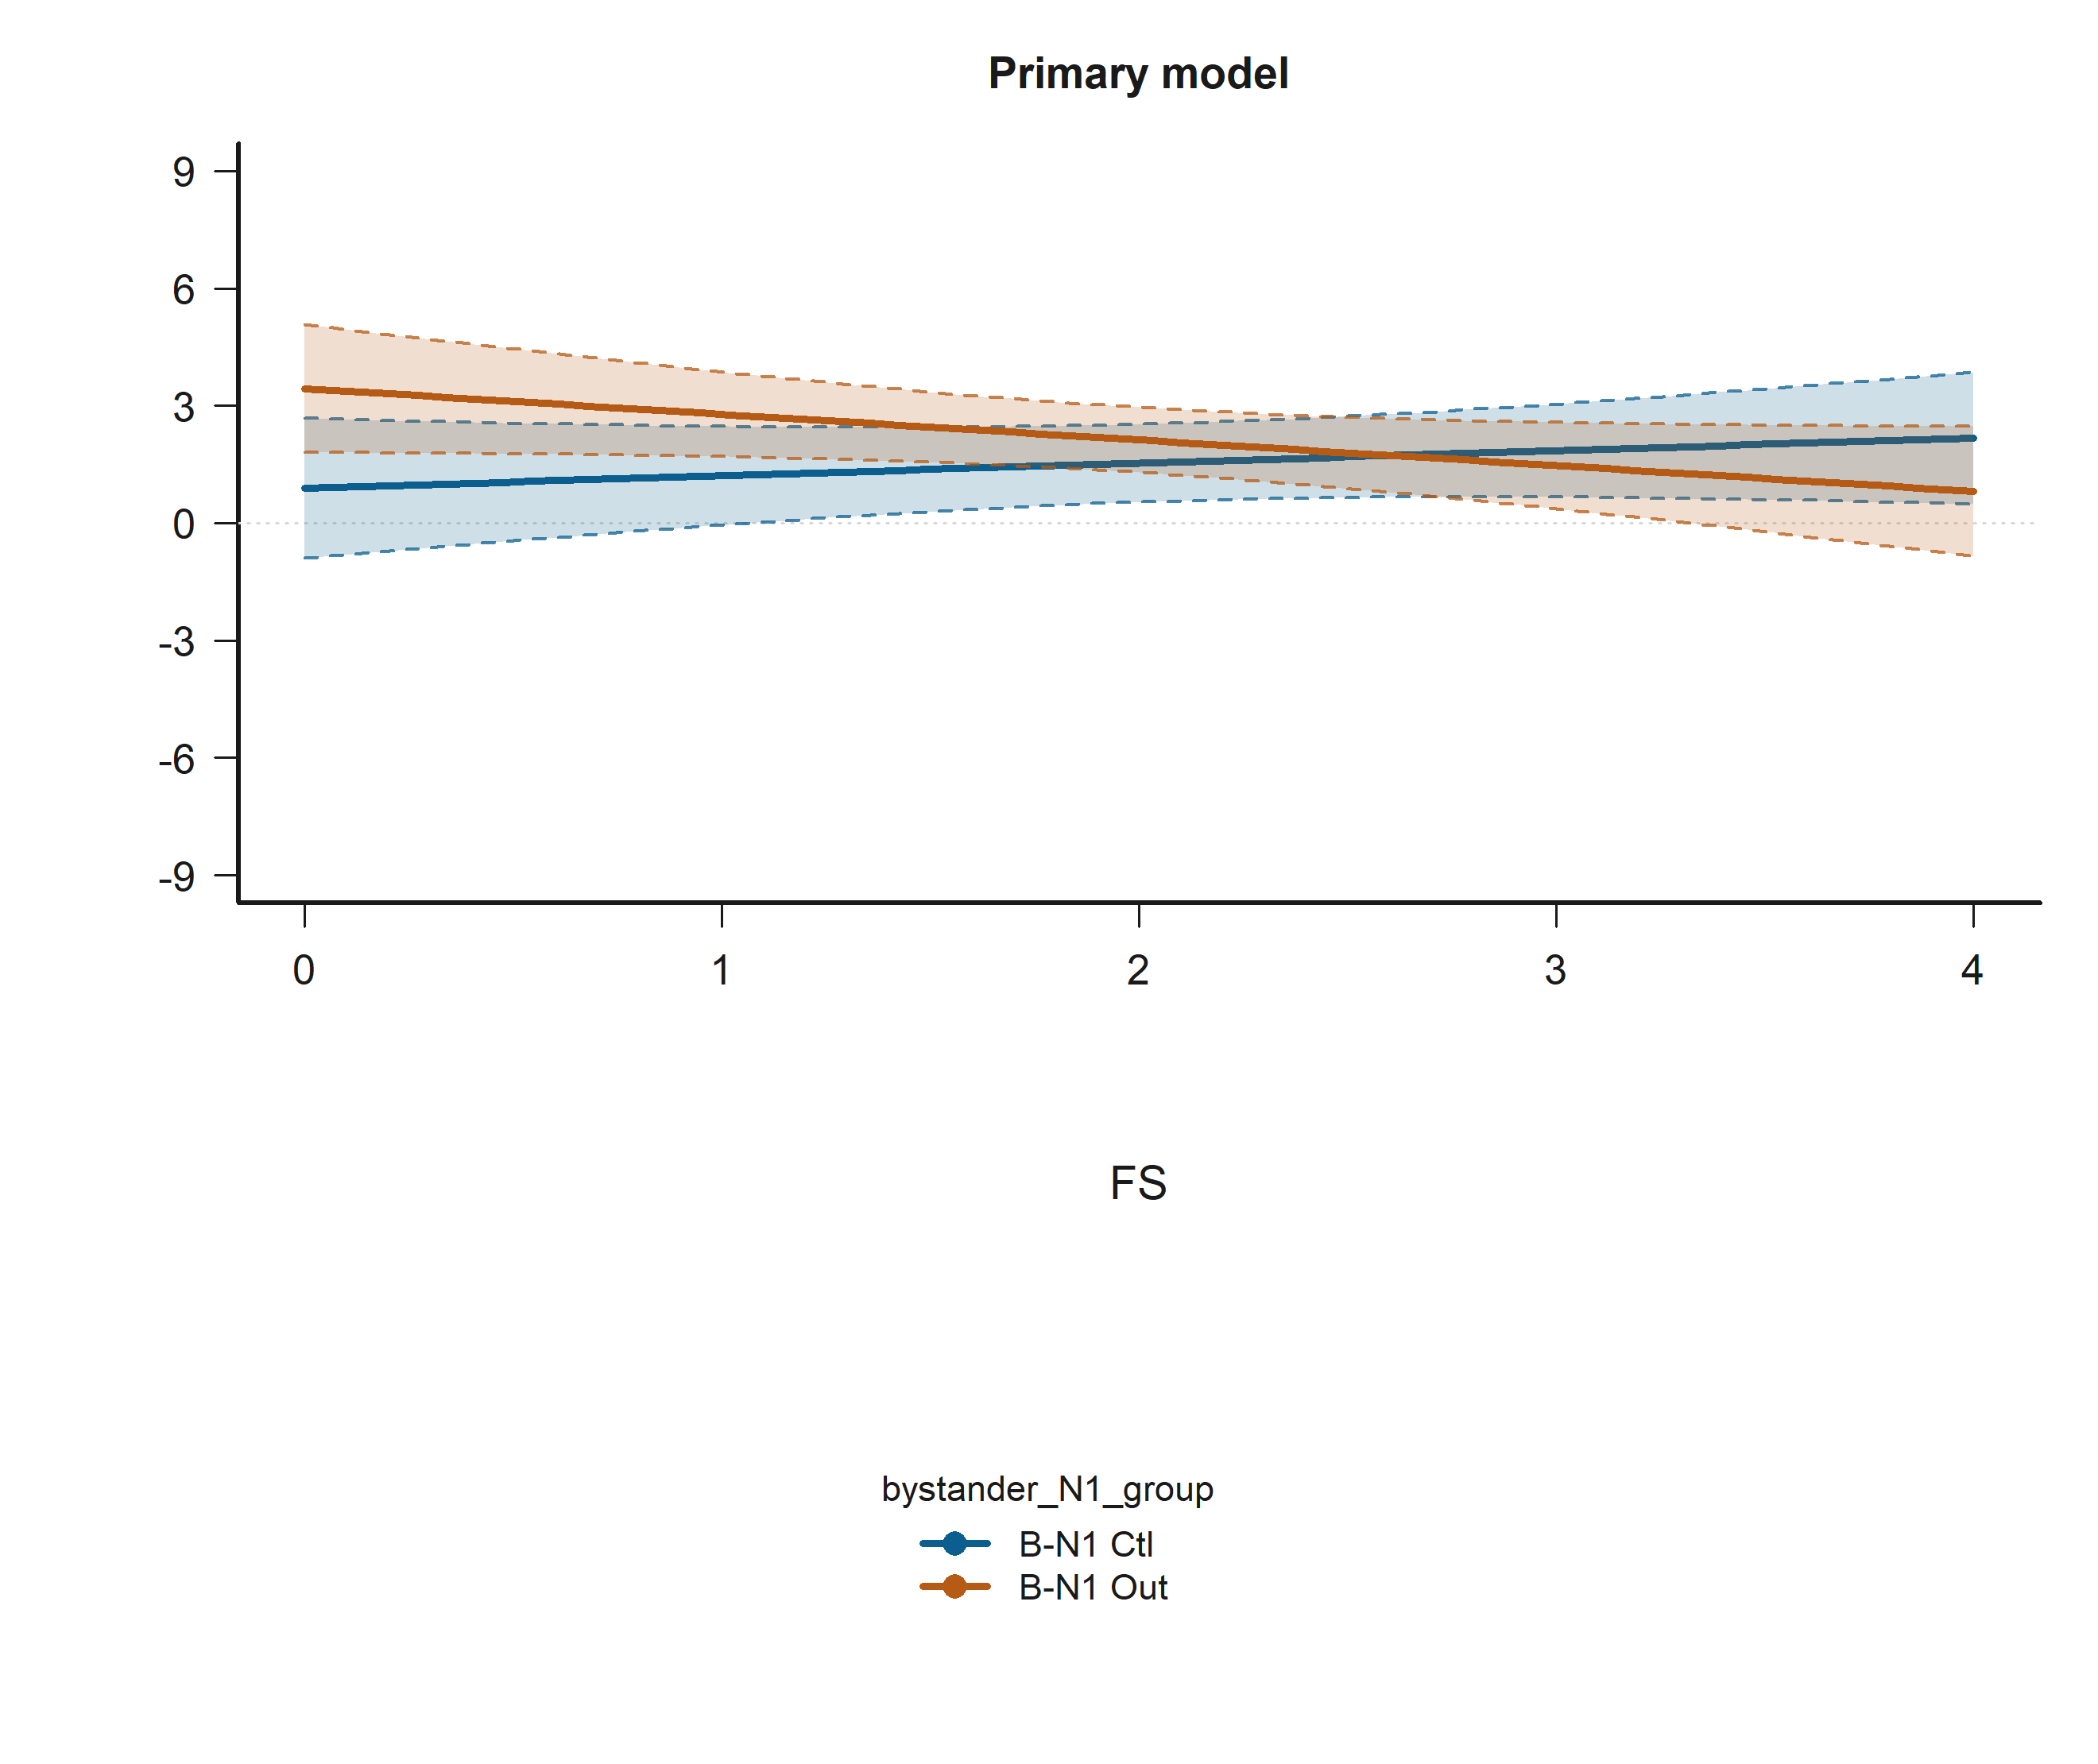
\includegraphics[width=0.92\textwidth]{../figures/figure_sig_all_judgments_bystander_bystander_n1_groupout_iri_fs_judgments_bystander_bystander_n1_outgroup_ref_control_x_empathy_fantasy_scale.png}
\caption{Interaction Plot for Bystander-N1: Outgroup (ref = Control) x Empathy: Fantasy scale in the judgments\_bystander. The panels show predicted judgments on the observed -9 to 9 scale with 95\% confidence intervals. Abbrev.: FS / EC / PT / PD = IRI subscales; N1 / N2 = negotiator 1 / negotiator 2; B-V = bystander-victim relation; V-N1 / V-N2 = victim-negotiator relations; B-N1 / B-N2 = bystander-negotiator relations; Vic / Obs = victim / observer subset; In / Out / Ctl = ingroup / outgroup / control label hidden; SameFac = N1 and N2 same faculty; SES = economic status.}
\label{fig:sig_all_judgments_bystander_bystander_n1_groupout_iri_fs}
\end{figure}

Empathy: Perspective taking is statistically significant in:
\begin{itemize}
  \item Empathy x Relational Status Model B (Tobit random-intercepts)
\end{itemize}
Figure \ref{fig:sig_all_judgments_bystander_iri_pt} shows that across the observed range, higher Empathy: Perspective taking corresponds to higher predicted judgment.

\begin{figure}[H]
\centering
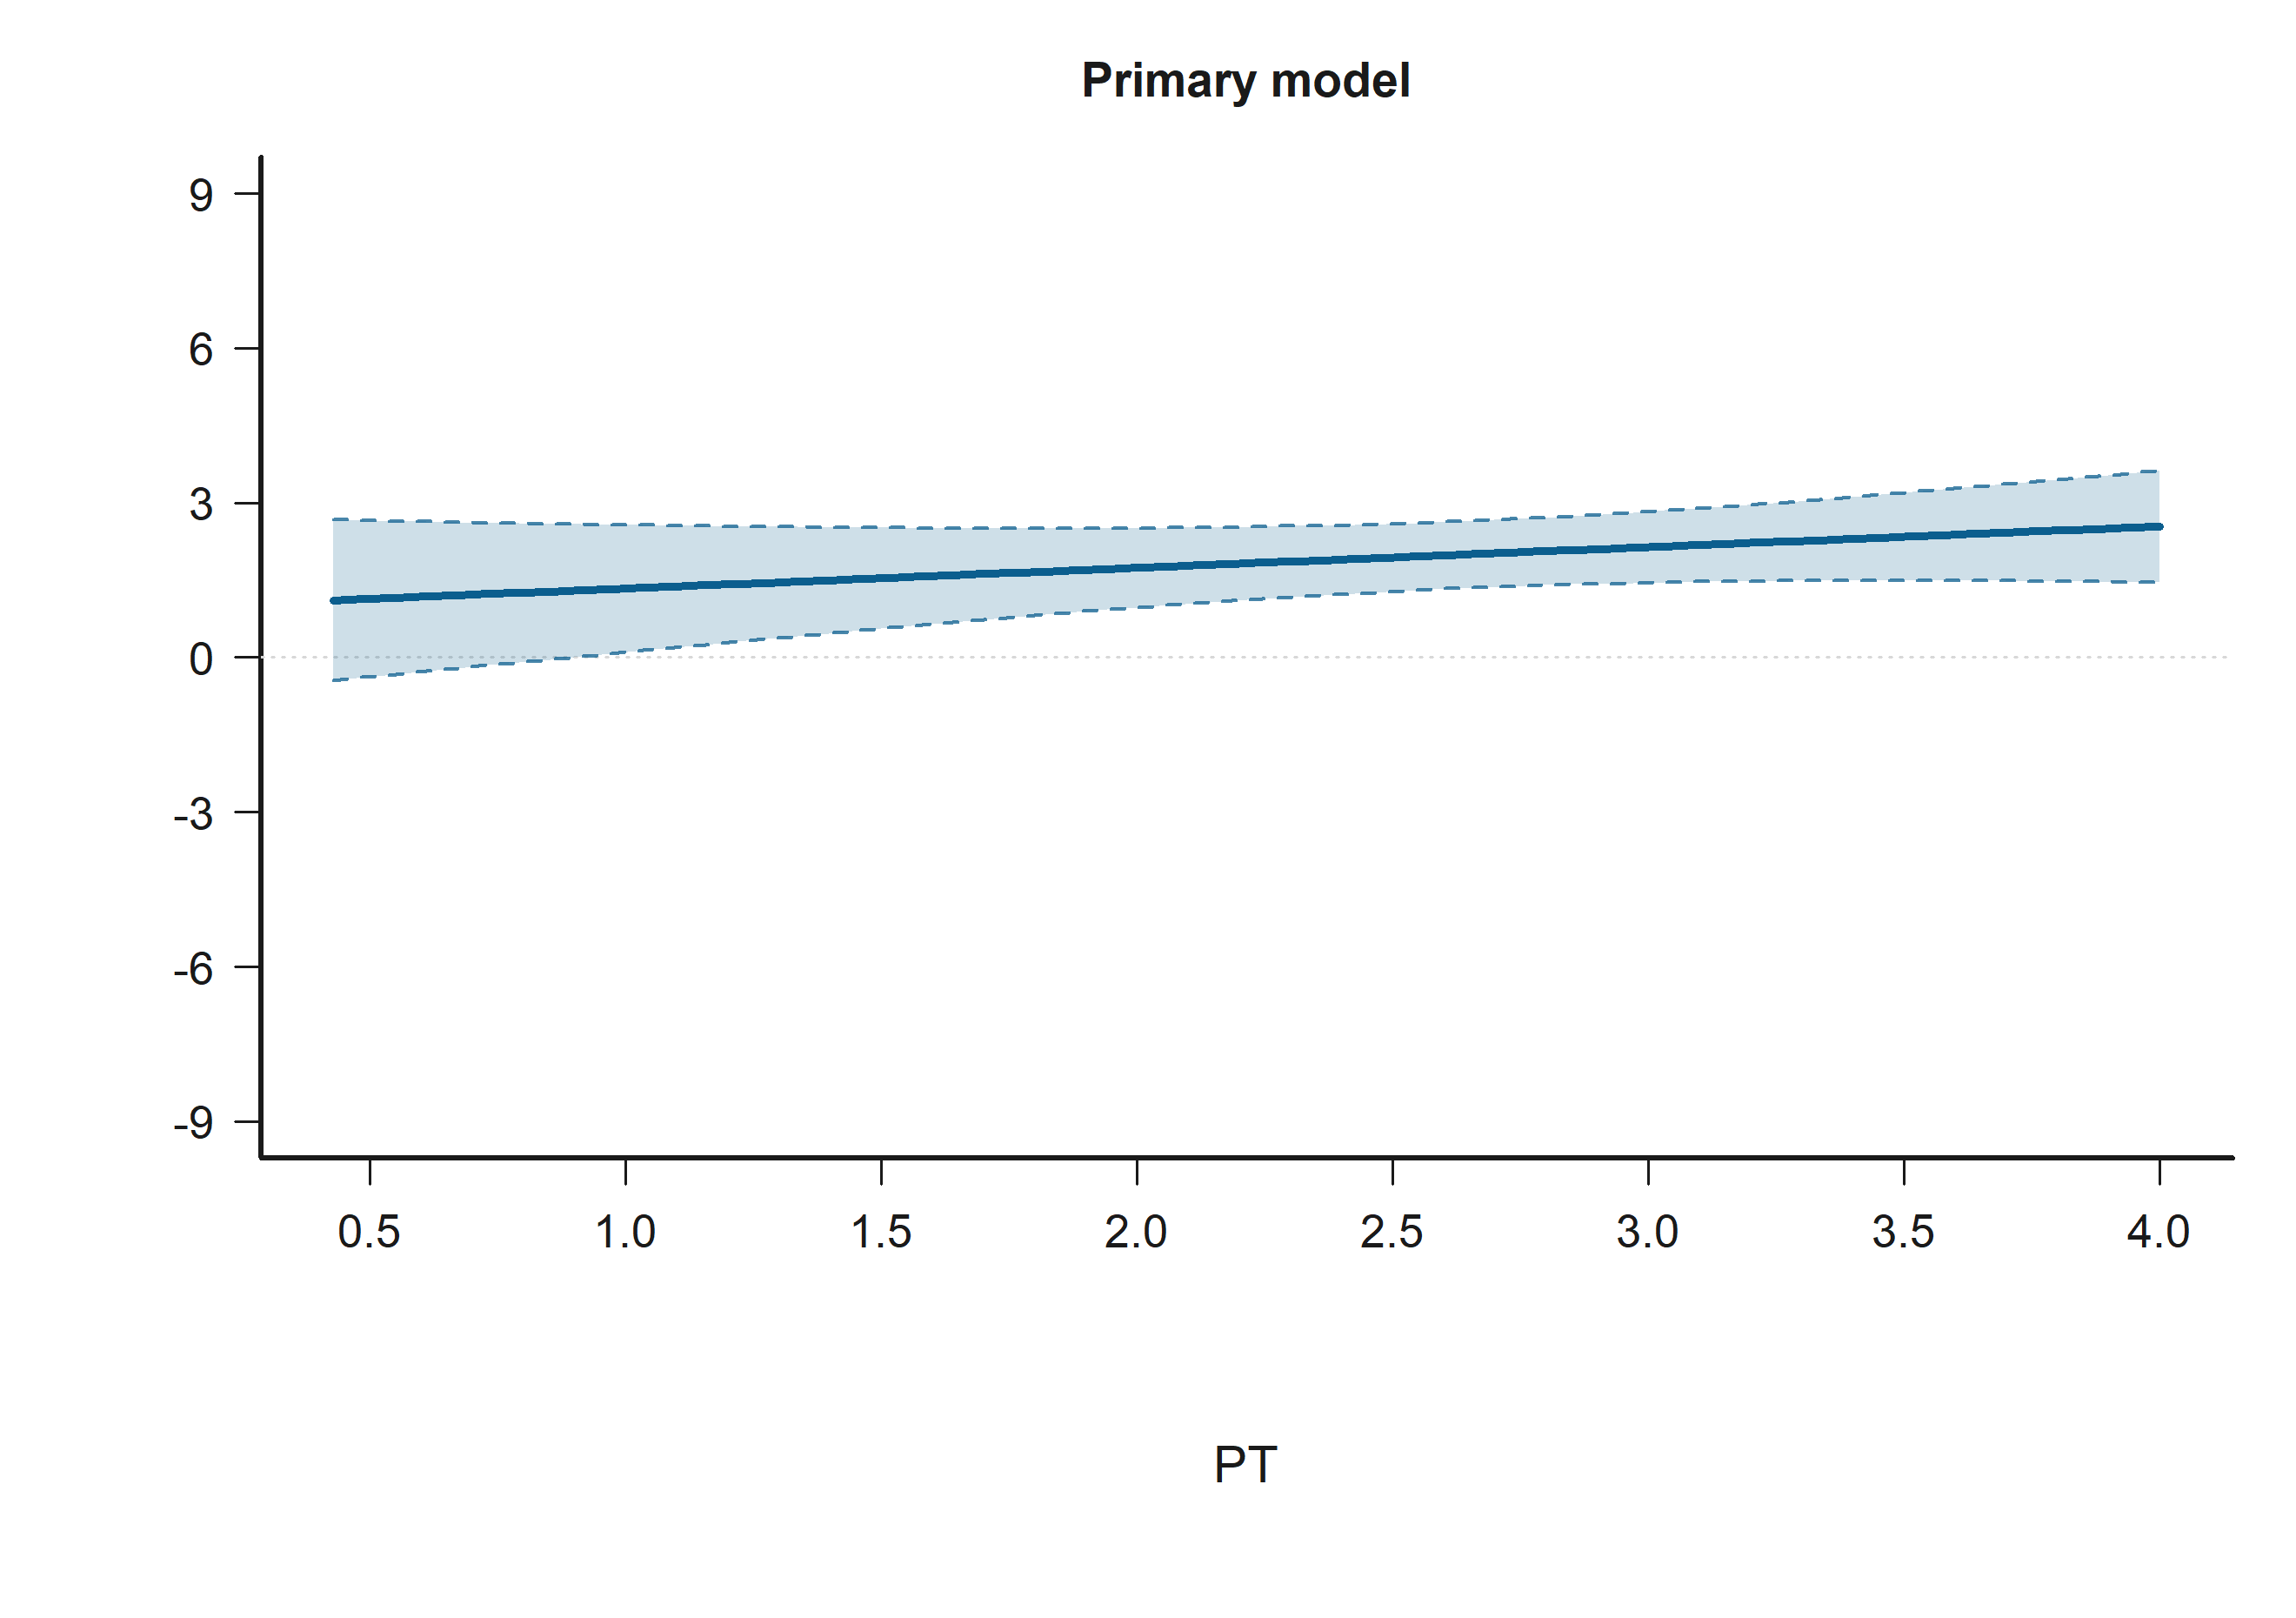
\includegraphics[width=0.92\textwidth]{../figures/figure_sig_all_judgments_bystander_iri_pt_judgments_bystander_empathy_perspective_taking.png}
\caption{Effect Plot for Empathy: Perspective taking in the judgments\_bystander. The panels show predicted judgments on the observed -9 to 9 scale with 95\% confidence intervals. Abbrev.: FS / EC / PT / PD = IRI subscales; N1 / N2 = negotiator 1 / negotiator 2; B-V = bystander-victim relation; V-N1 / V-N2 = victim-negotiator relations; B-N1 / B-N2 = bystander-negotiator relations; Vic / Obs = victim / observer subset; In / Out / Ctl = ingroup / outgroup / control label hidden; SameFac = N1 and N2 same faculty; SES = economic status.}
\label{fig:sig_all_judgments_bystander_iri_pt}
\end{figure}

Bystander-N2: Ingroup (ref = Control) is statistically significant in:
\begin{itemize}
  \item Empathy Effect Model B (Tobit random-intercepts)
  \item Negotiator-Side Structure Model B (Tobit random-intercepts)
\end{itemize}
Figure \ref{fig:sig_all_judgments_bystander_bystander_n2_groupin} shows that predicted judgment is lower for B-N2 In than for B-N2 Ctl.

\begin{figure}[H]
\centering
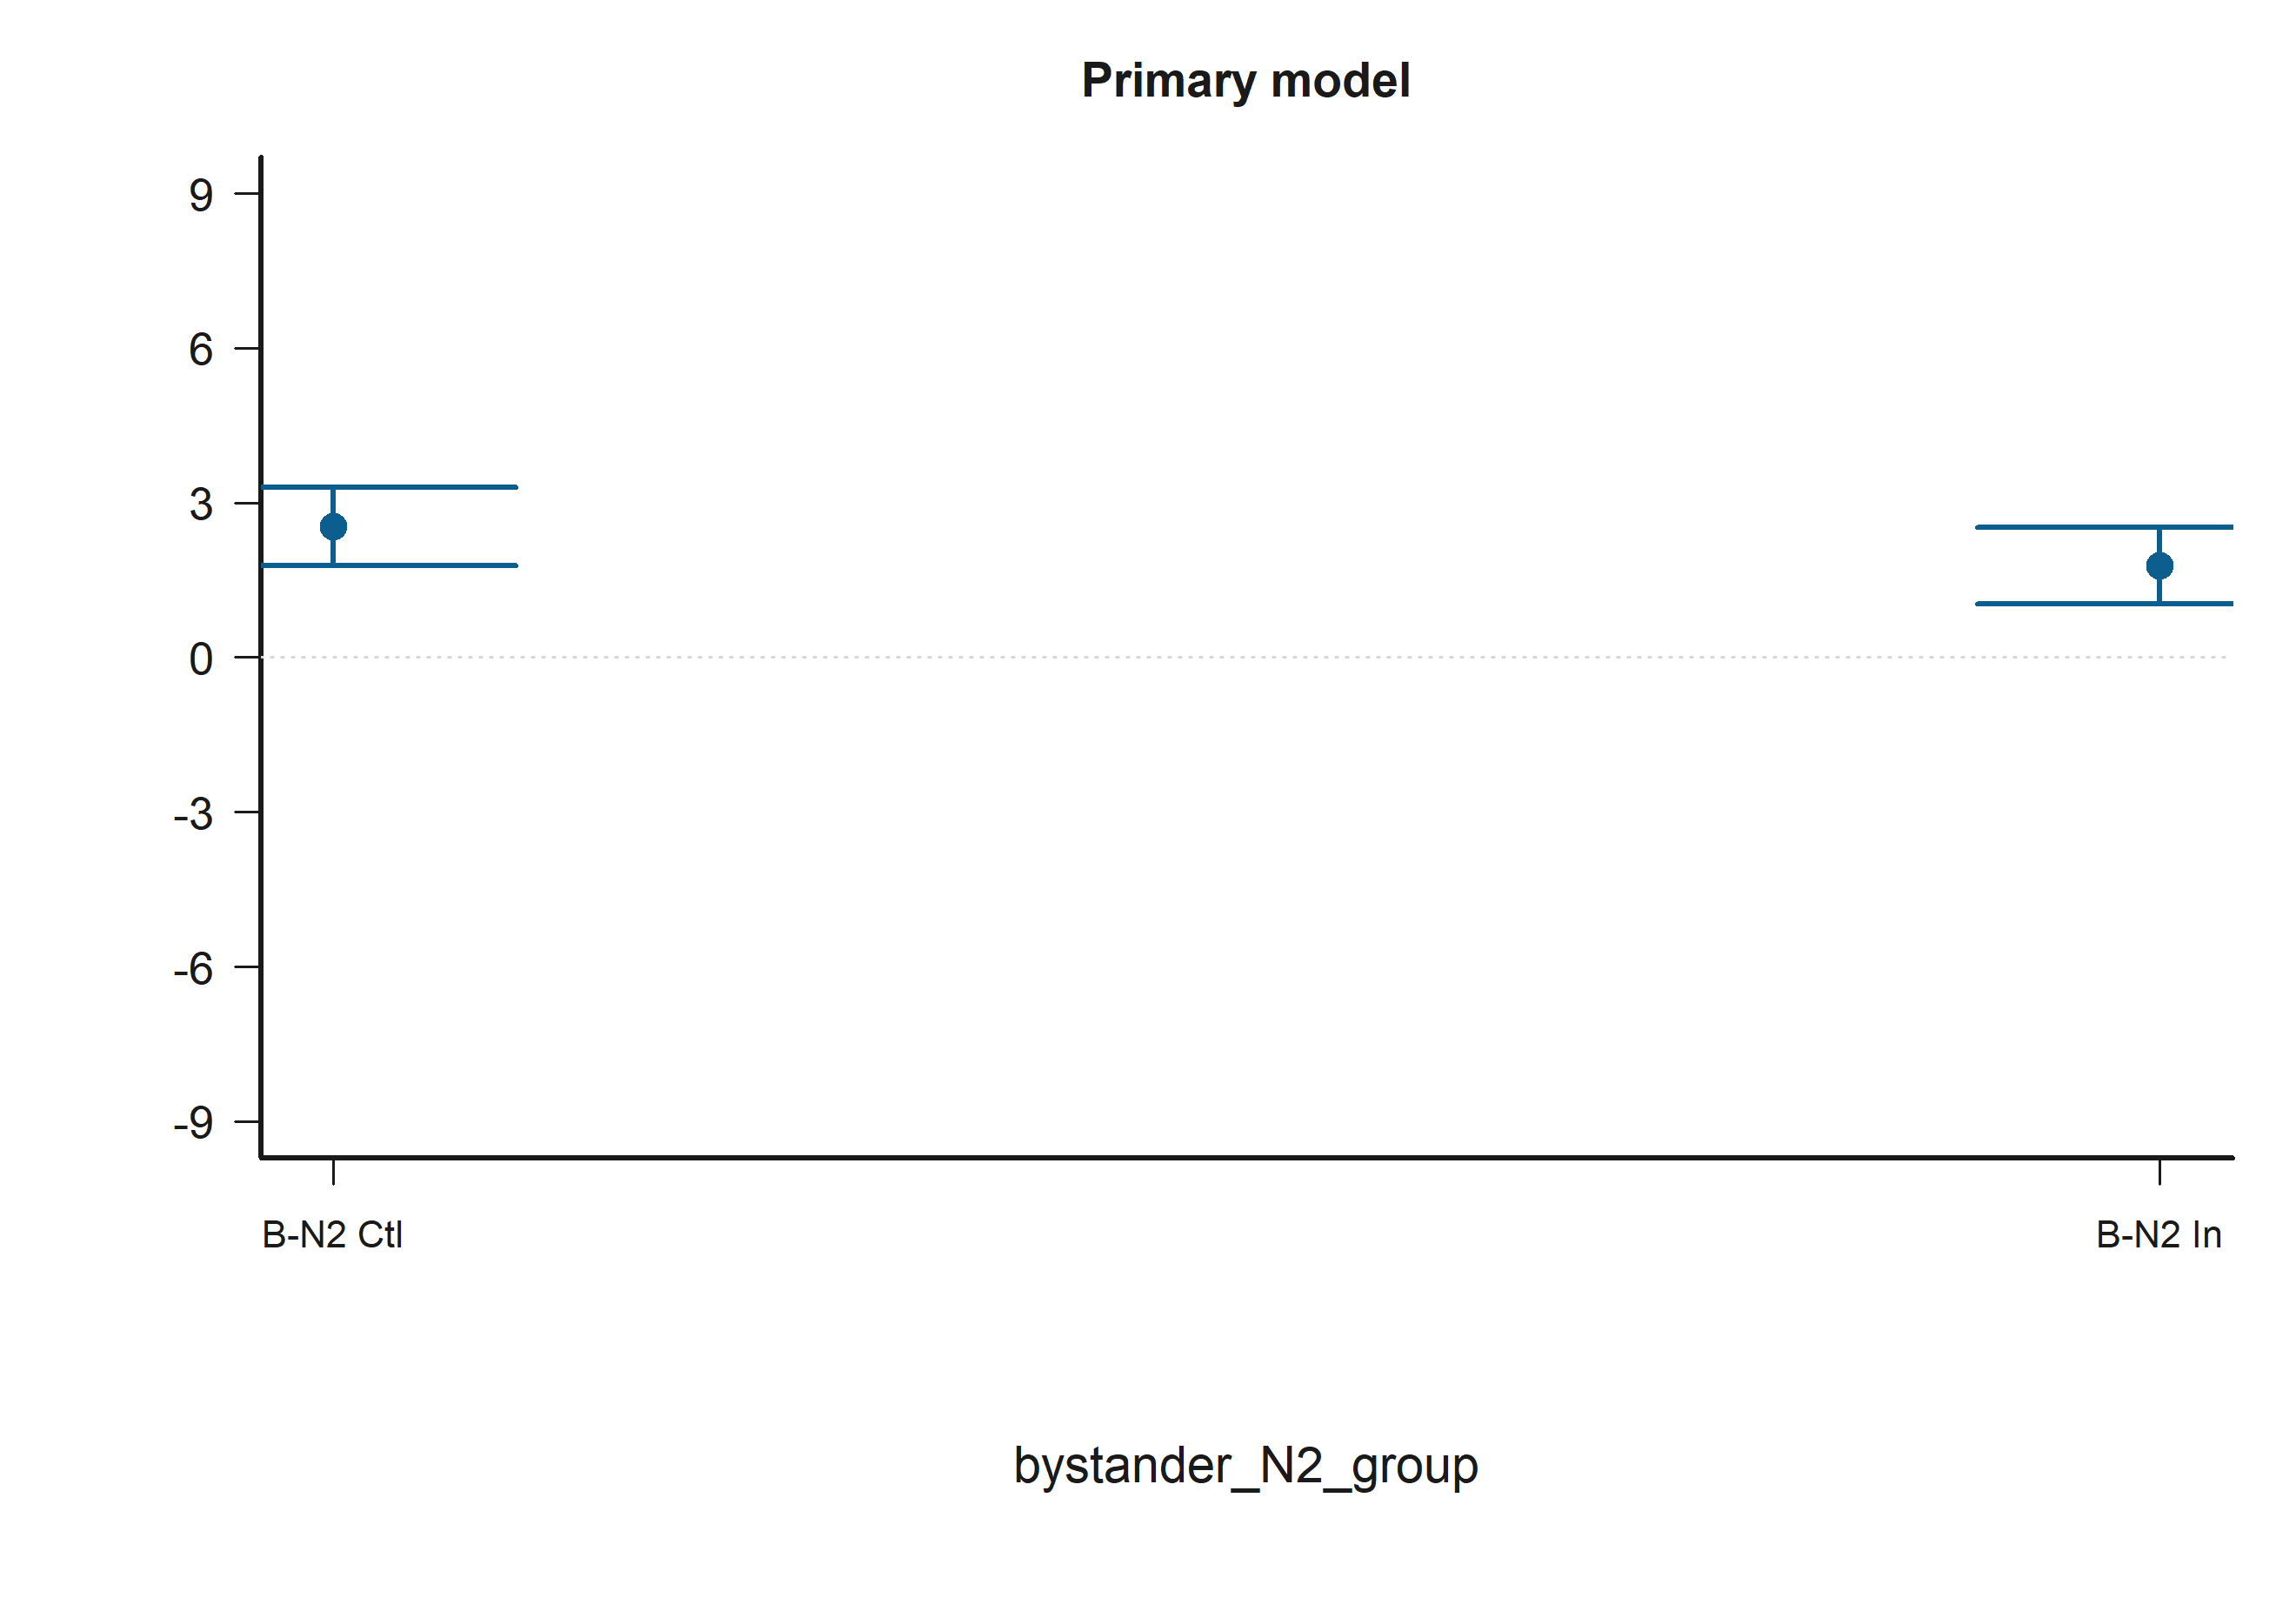
\includegraphics[width=0.92\textwidth]{../figures/figure_sig_all_judgments_bystander_bystander_n2_groupin_judgments_bystander_bystander_n2_ingroup_ref_control.png}
\caption{Grouped Prediction Plot for Bystander-N2: Ingroup (ref = Control) in the judgments\_bystander. The panels show predicted judgments on the observed -9 to 9 scale with 95\% confidence intervals. Abbrev.: FS / EC / PT / PD = IRI subscales; N1 / N2 = negotiator 1 / negotiator 2; B-V = bystander-victim relation; V-N1 / V-N2 = victim-negotiator relations; B-N1 / B-N2 = bystander-negotiator relations; Vic / Obs = victim / observer subset; In / Out / Ctl = ingroup / outgroup / control label hidden; SameFac = N1 and N2 same faculty; SES = economic status.}
\label{fig:sig_all_judgments_bystander_bystander_n2_groupin}
\end{figure}

Bystander-N1: Ingroup (ref = Control) is statistically significant in:
\begin{itemize}
  \item Empathy x Relational Status Model B (Tobit random-intercepts)
  \item Empathy Effect Model B (Tobit random-intercepts)
\end{itemize}
Figure \ref{fig:sig_all_judgments_bystander_bystander_n1_groupin} shows that predicted judgment is higher for B-N1 In than for B-N1 Ctl.

\begin{figure}[H]
\centering
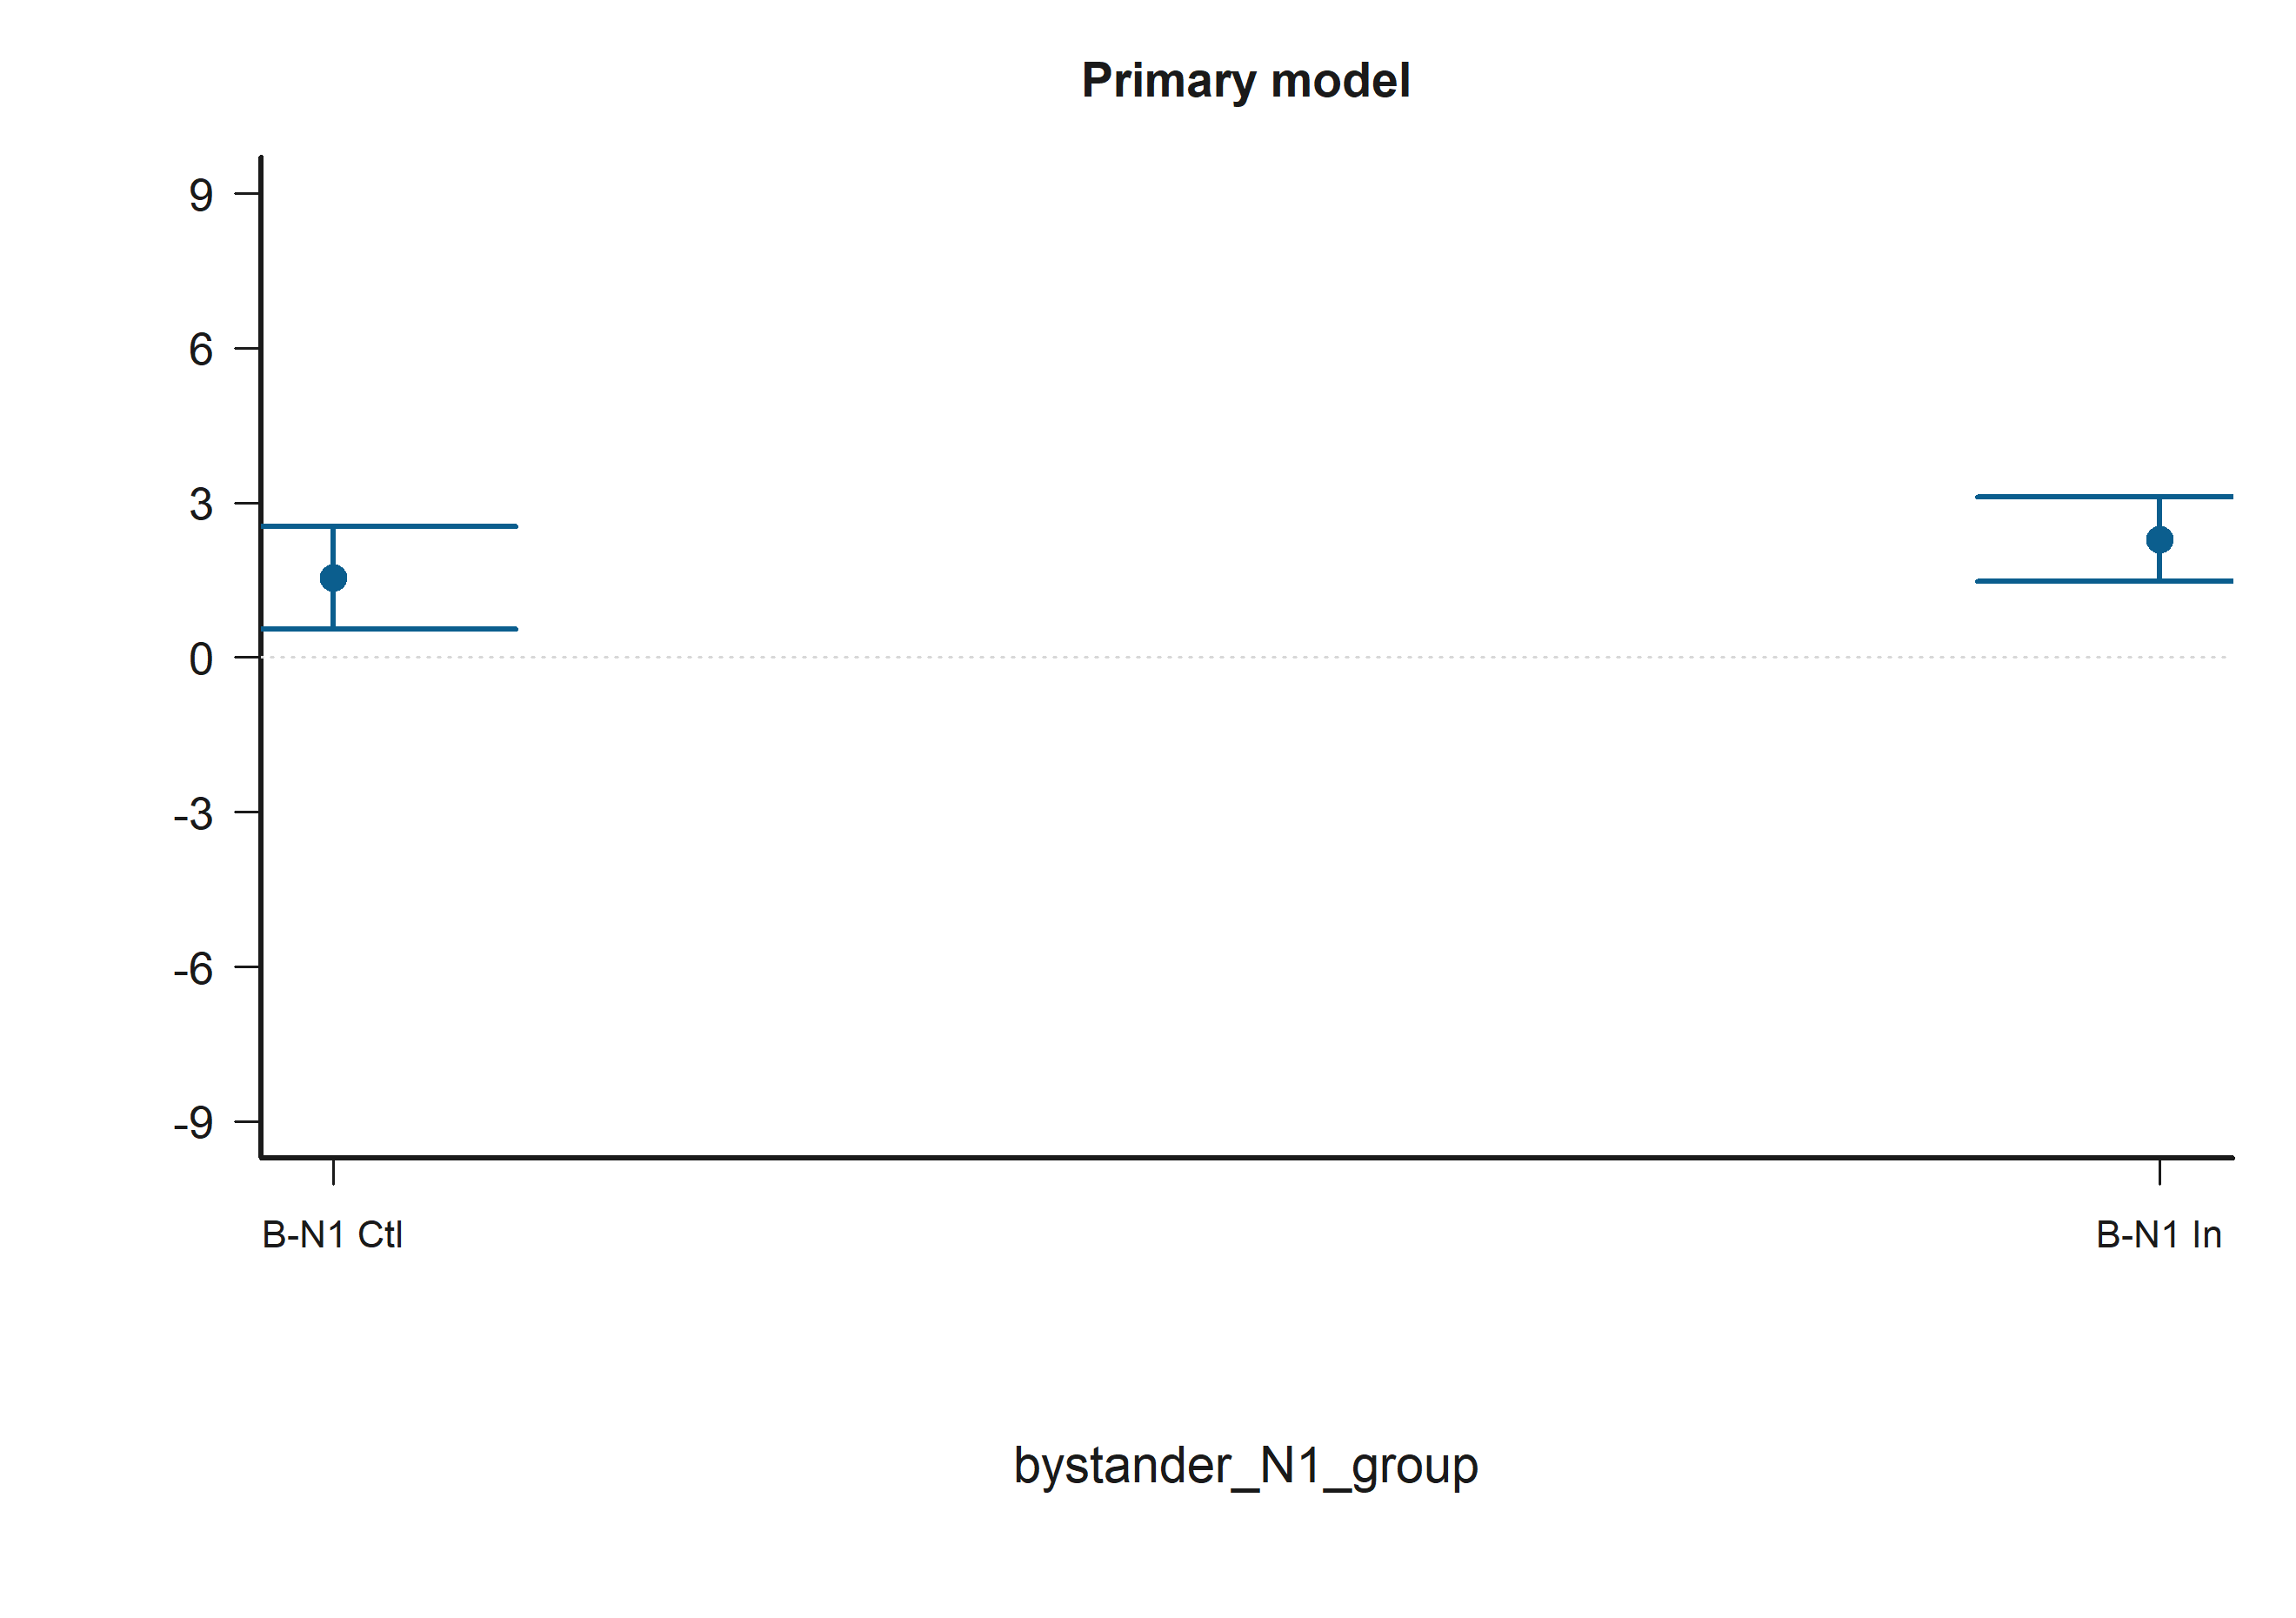
\includegraphics[width=0.92\textwidth]{../figures/figure_sig_all_judgments_bystander_bystander_n1_groupin_judgments_bystander_bystander_n1_ingroup_ref_control.png}
\caption{Grouped Prediction Plot for Bystander-N1: Ingroup (ref = Control) in the judgments\_bystander. The panels show predicted judgments on the observed -9 to 9 scale with 95\% confidence intervals. Abbrev.: FS / EC / PT / PD = IRI subscales; N1 / N2 = negotiator 1 / negotiator 2; B-V = bystander-victim relation; V-N1 / V-N2 = victim-negotiator relations; B-N1 / B-N2 = bystander-negotiator relations; Vic / Obs = victim / observer subset; In / Out / Ctl = ingroup / outgroup / control label hidden; SameFac = N1 and N2 same faculty; SES = economic status.}
\label{fig:sig_all_judgments_bystander_bystander_n1_groupin}
\end{figure}

Victim-N2: Ingroup (ref = Control) is statistically significant in:
\begin{itemize}
  \item Empathy x Relational Status Model B (Tobit random-intercepts)
  \item Negotiator-Side Structure Model B (Tobit random-intercepts)
\end{itemize}
Figure \ref{fig:sig_all_judgments_bystander_victim_n2_groupin} shows that predicted judgment is higher for V-N2 In than for V-N2 Ctl.

\begin{figure}[H]
\centering
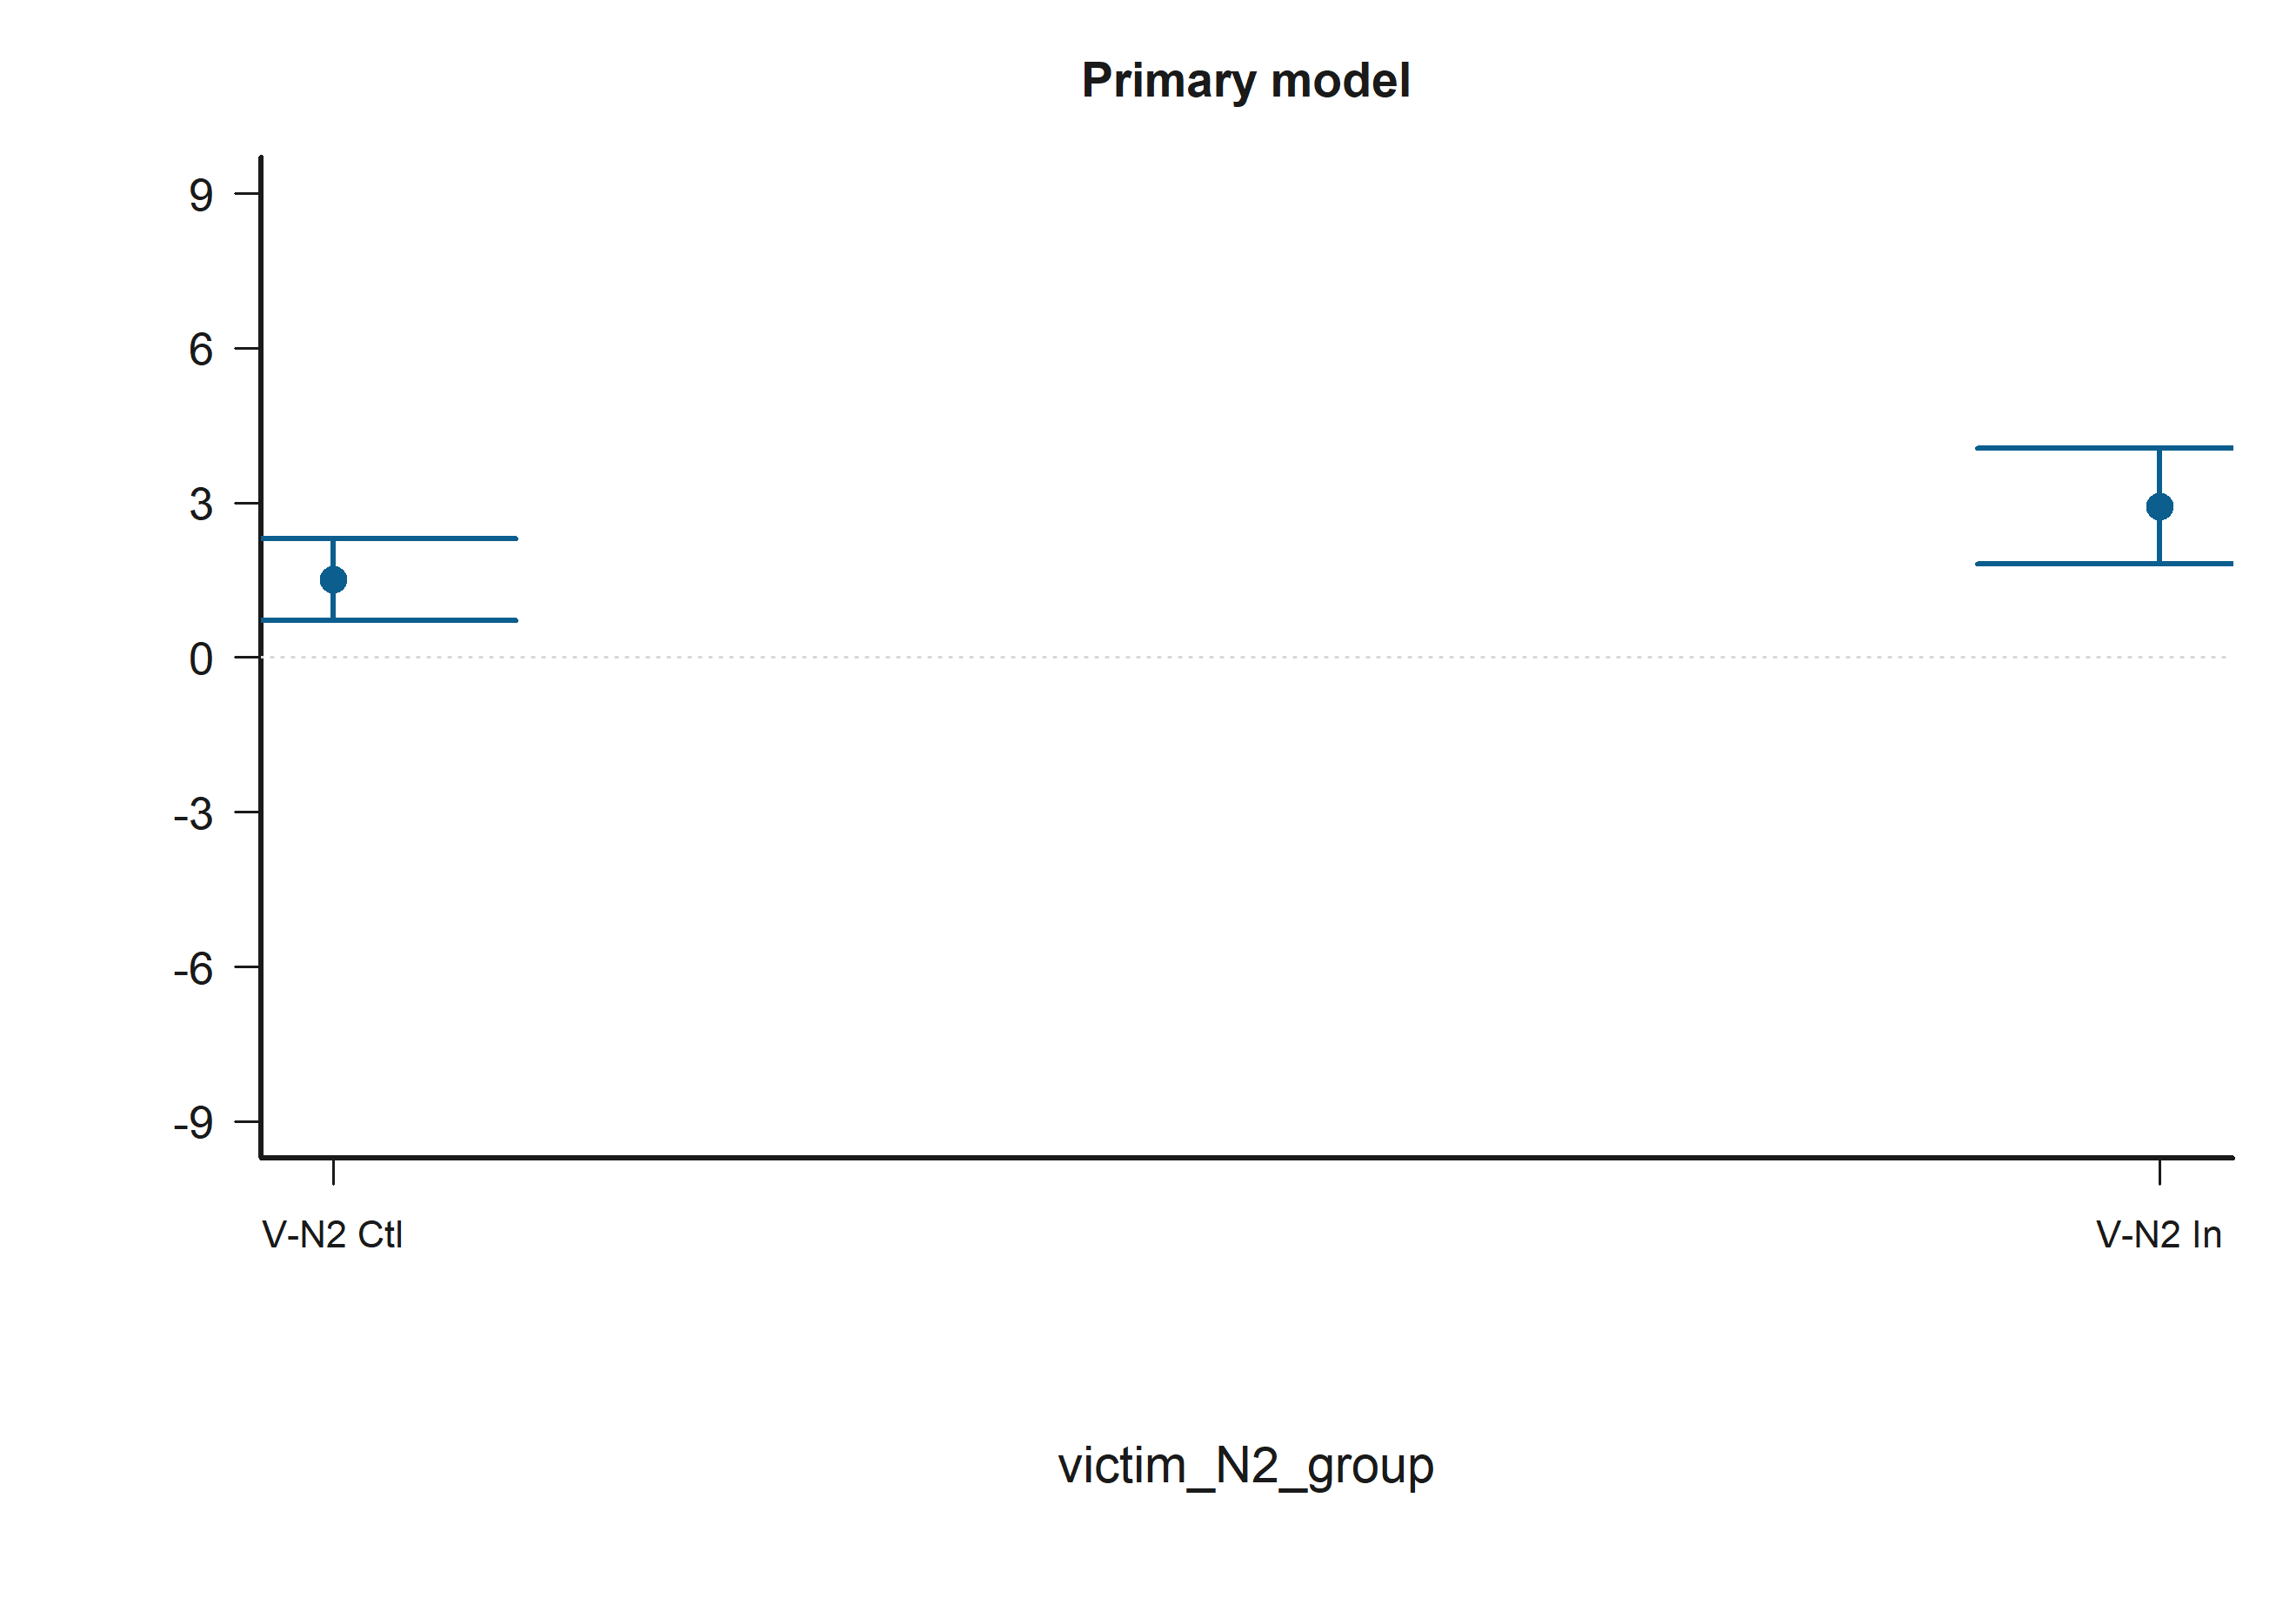
\includegraphics[width=0.92\textwidth]{../figures/figure_sig_all_judgments_bystander_victim_n2_groupin_judgments_bystander_victim_n2_ingroup_ref_control.png}
\caption{Grouped Prediction Plot for Victim-N2: Ingroup (ref = Control) in the judgments\_bystander. The panels show predicted judgments on the observed -9 to 9 scale with 95\% confidence intervals. Abbrev.: FS / EC / PT / PD = IRI subscales; N1 / N2 = negotiator 1 / negotiator 2; B-V = bystander-victim relation; V-N1 / V-N2 = victim-negotiator relations; B-N1 / B-N2 = bystander-negotiator relations; Vic / Obs = victim / observer subset; In / Out / Ctl = ingroup / outgroup / control label hidden; SameFac = N1 and N2 same faculty; SES = economic status.}
\label{fig:sig_all_judgments_bystander_victim_n2_groupin}
\end{figure}

Bystander-victim: Outgroup (ref = Ingroup) x Empathy: Personal distress is statistically significant in:
\begin{itemize}
  \item Empathy x Relational Status Model B (Tobit random-intercepts)
\end{itemize}
Figure \ref{fig:sig_all_judgments_bystander_bystander_victim_groupout_iri_pd} shows that the predicted relationship rises most sharply for Empathy: Personal distress when the condition is B-V Out.

\begin{figure}[H]
\centering
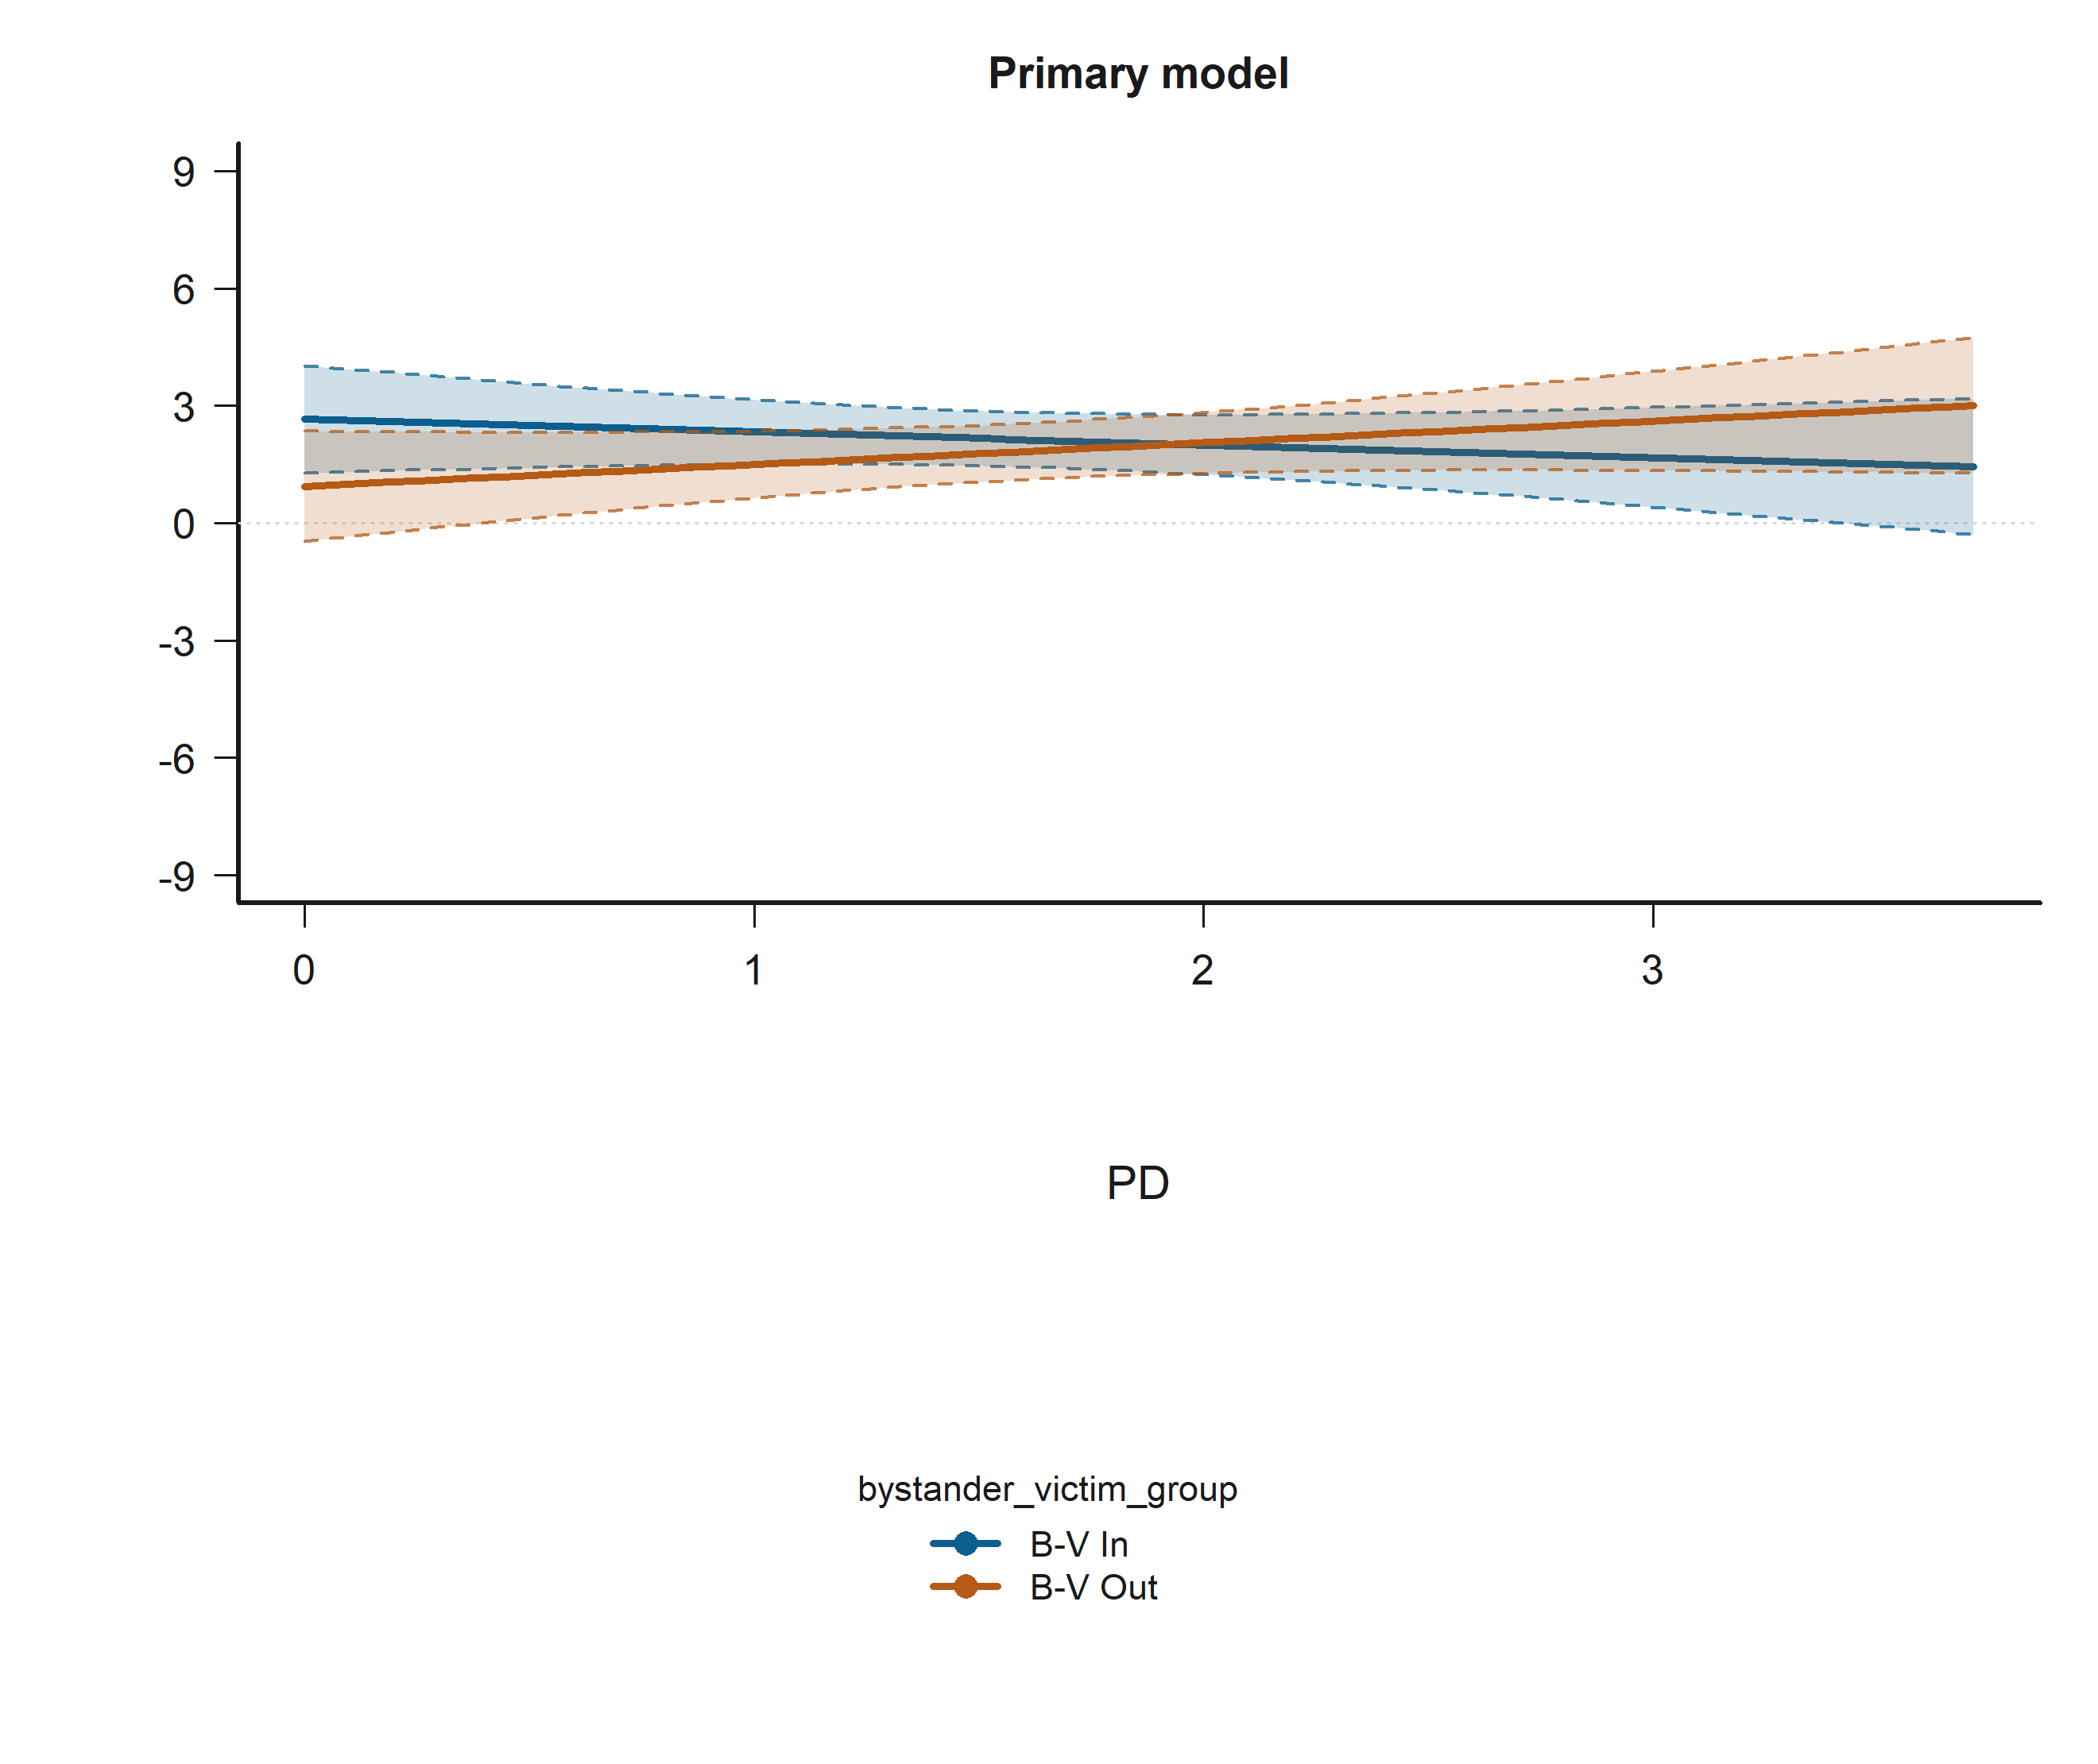
\includegraphics[width=0.92\textwidth]{../figures/figure_sig_all_judgments_bystander_bystander_victim_groupout_iri_pd_judgments_bystander_bystander_victim_outgroup_ref_ingroup_x_empathy_personal_distress.png}
\caption{Interaction Plot for Bystander-victim: Outgroup (ref = Ingroup) x Empathy: Personal distress in the judgments\_bystander. The panels show predicted judgments on the observed -9 to 9 scale with 95\% confidence intervals. Abbrev.: FS / EC / PT / PD = IRI subscales; N1 / N2 = negotiator 1 / negotiator 2; B-V = bystander-victim relation; V-N1 / V-N2 = victim-negotiator relations; B-N1 / B-N2 = bystander-negotiator relations; Vic / Obs = victim / observer subset; In / Out / Ctl = ingroup / outgroup / control label hidden; SameFac = N1 and N2 same faculty; SES = economic status.}
\label{fig:sig_all_judgments_bystander_bystander_victim_groupout_iri_pd}
\end{figure}

Bystander-N2: Outgroup (ref = Control) is statistically significant in:
\begin{itemize}
  \item Negotiator-Side Structure Model B (Tobit random-intercepts)
  \item Empathy Effect Model B (Tobit random-intercepts)
\end{itemize}
Figure \ref{fig:sig_all_judgments_bystander_bystander_n2_groupout} shows that predicted judgment is lower for B-N2 Out than for B-N2 Ctl.

\begin{figure}[H]
\centering
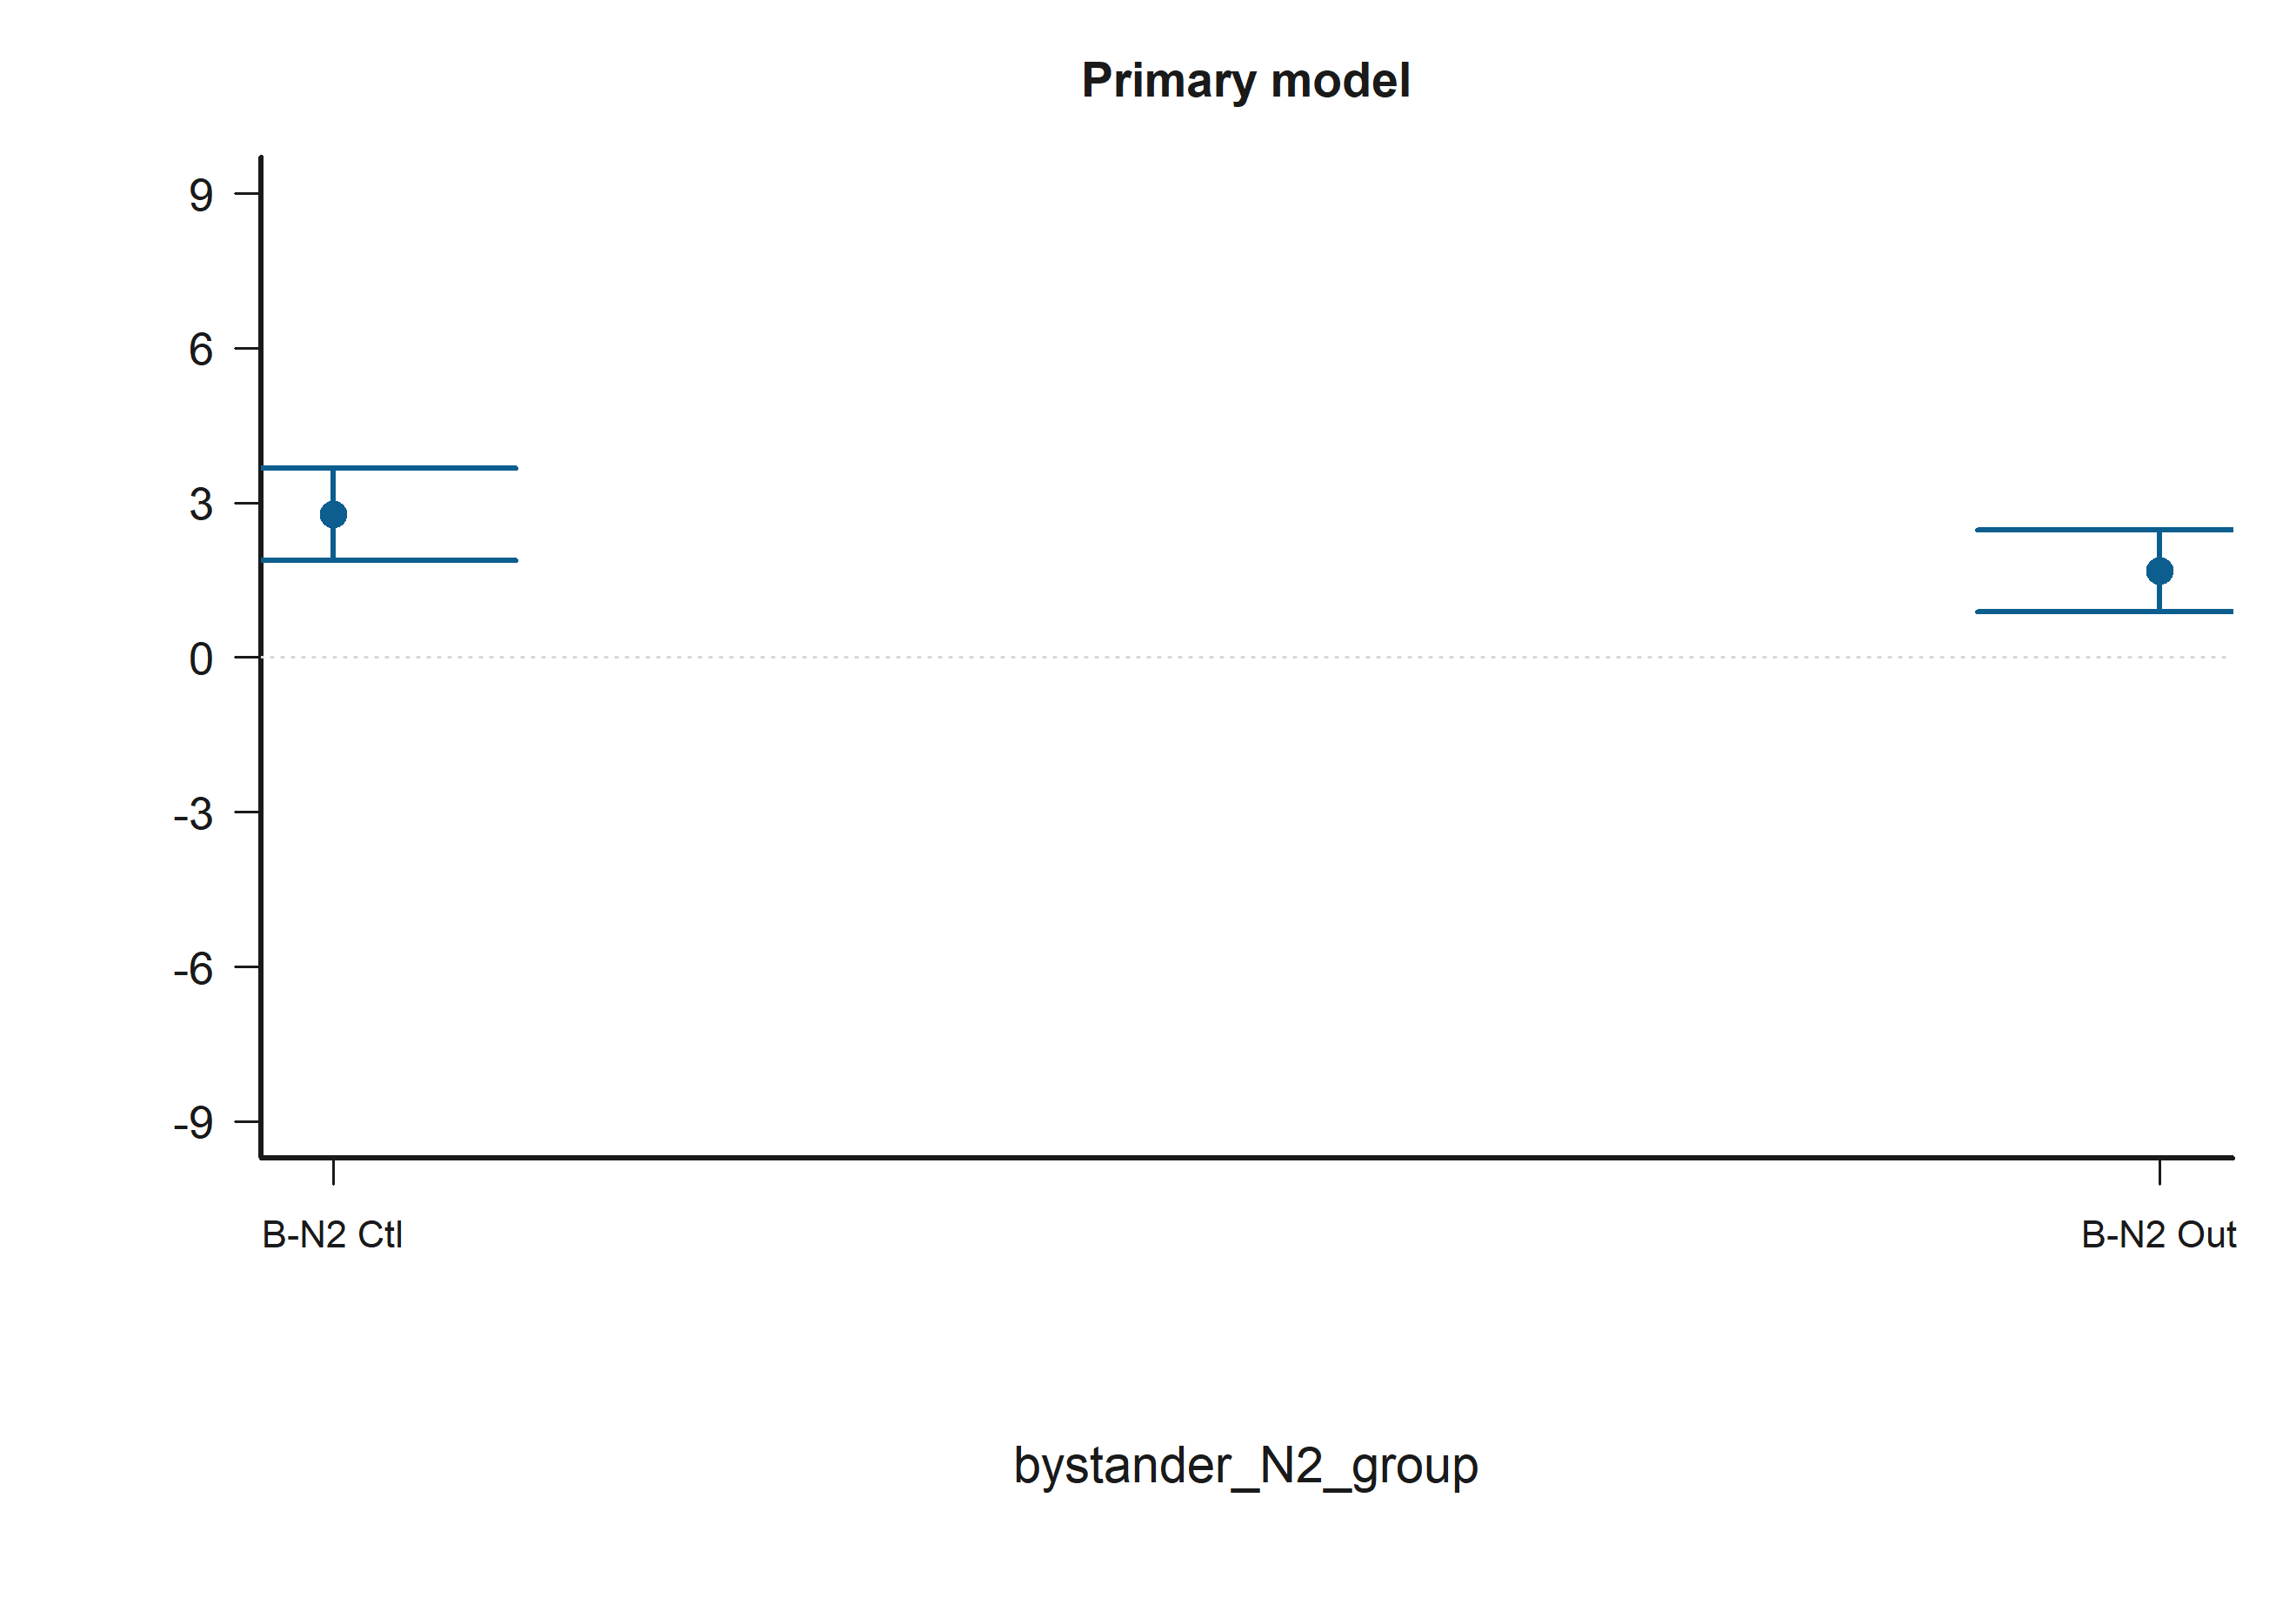
\includegraphics[width=0.92\textwidth]{../figures/figure_sig_all_judgments_bystander_bystander_n2_groupout_judgments_bystander_bystander_n2_outgroup_ref_control.png}
\caption{Grouped Prediction Plot for Bystander-N2: Outgroup (ref = Control) in the judgments\_bystander. The panels show predicted judgments on the observed -9 to 9 scale with 95\% confidence intervals. Abbrev.: FS / EC / PT / PD = IRI subscales; N1 / N2 = negotiator 1 / negotiator 2; B-V = bystander-victim relation; V-N1 / V-N2 = victim-negotiator relations; B-N1 / B-N2 = bystander-negotiator relations; Vic / Obs = victim / observer subset; In / Out / Ctl = ingroup / outgroup / control label hidden; SameFac = N1 and N2 same faculty; SES = economic status.}
\label{fig:sig_all_judgments_bystander_bystander_n2_groupout}
\end{figure}

Bystander-N2: Outgroup (ref = Control) x Empathy: Perspective taking is statistically significant in:
\begin{itemize}
  \item Empathy x Relational Status Model B (Tobit random-intercepts)
\end{itemize}
Figure \ref{fig:sig_all_judgments_bystander_bystander_n2_groupout_iri_pt} shows that the predicted relationship rises most sharply for Empathy: Perspective taking when the condition is B-N2 Ctl.

\begin{figure}[H]
\centering
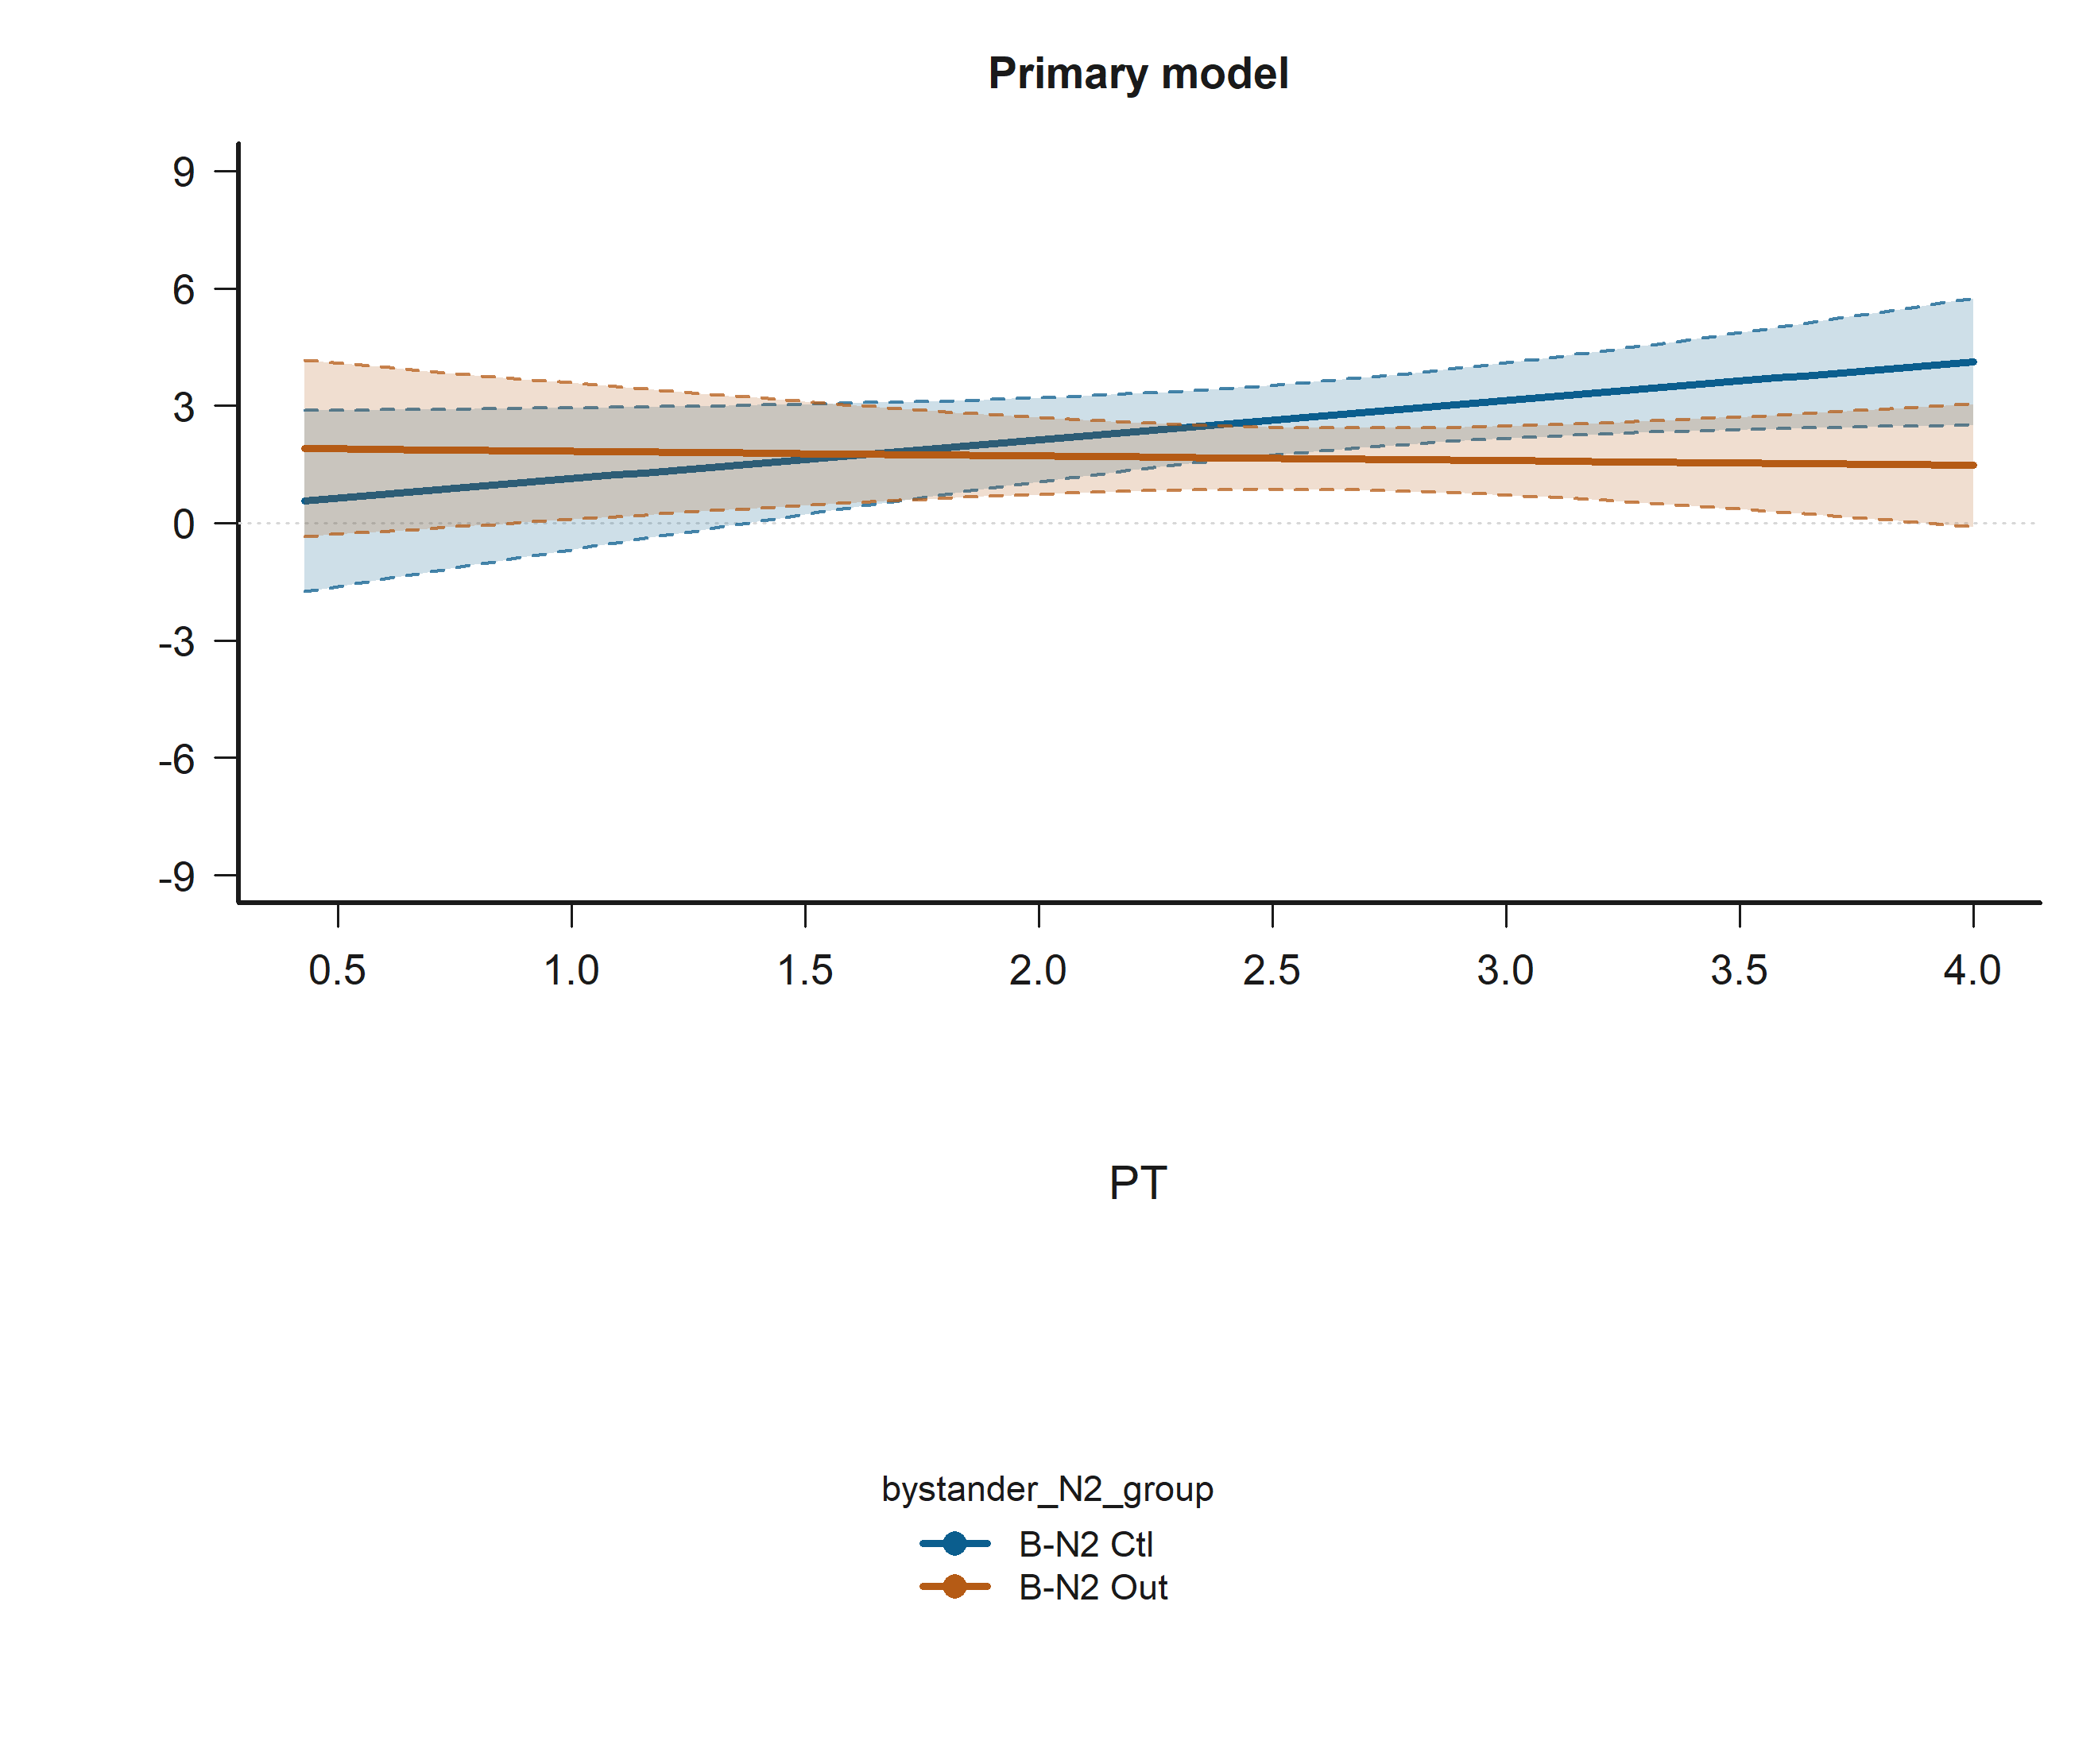
\includegraphics[width=0.92\textwidth]{../figures/figure_sig_all_judgments_bystander_bystander_n2_groupout_iri_pt_judgments_bystander_bystander_n2_outgroup_ref_control_x_empathy_perspective_taking.png}
\caption{Interaction Plot for Bystander-N2: Outgroup (ref = Control) x Empathy: Perspective taking in the judgments\_bystander. The panels show predicted judgments on the observed -9 to 9 scale with 95\% confidence intervals. Abbrev.: FS / EC / PT / PD = IRI subscales; N1 / N2 = negotiator 1 / negotiator 2; B-V = bystander-victim relation; V-N1 / V-N2 = victim-negotiator relations; B-N1 / B-N2 = bystander-negotiator relations; Vic / Obs = victim / observer subset; In / Out / Ctl = ingroup / outgroup / control label hidden; SameFac = N1 and N2 same faculty; SES = economic status.}
\label{fig:sig_all_judgments_bystander_bystander_n2_groupout_iri_pt}
\end{figure}

Bystander-N1: Outgroup (ref = Control) x Bystander-N2: Ingroup (ref = Control) is statistically significant in:
\begin{itemize}
  \item Empathy x Relational Status Model B (Tobit random-intercepts)
\end{itemize}
Figure \ref{fig:sig_all_judgments_bystander_bystander_n1_groupout_bystander_n2_groupin} shows that the predicted relationship rises most sharply for bystander\_N1\_group when the condition is B-N2 In.

\begin{figure}[H]
\centering
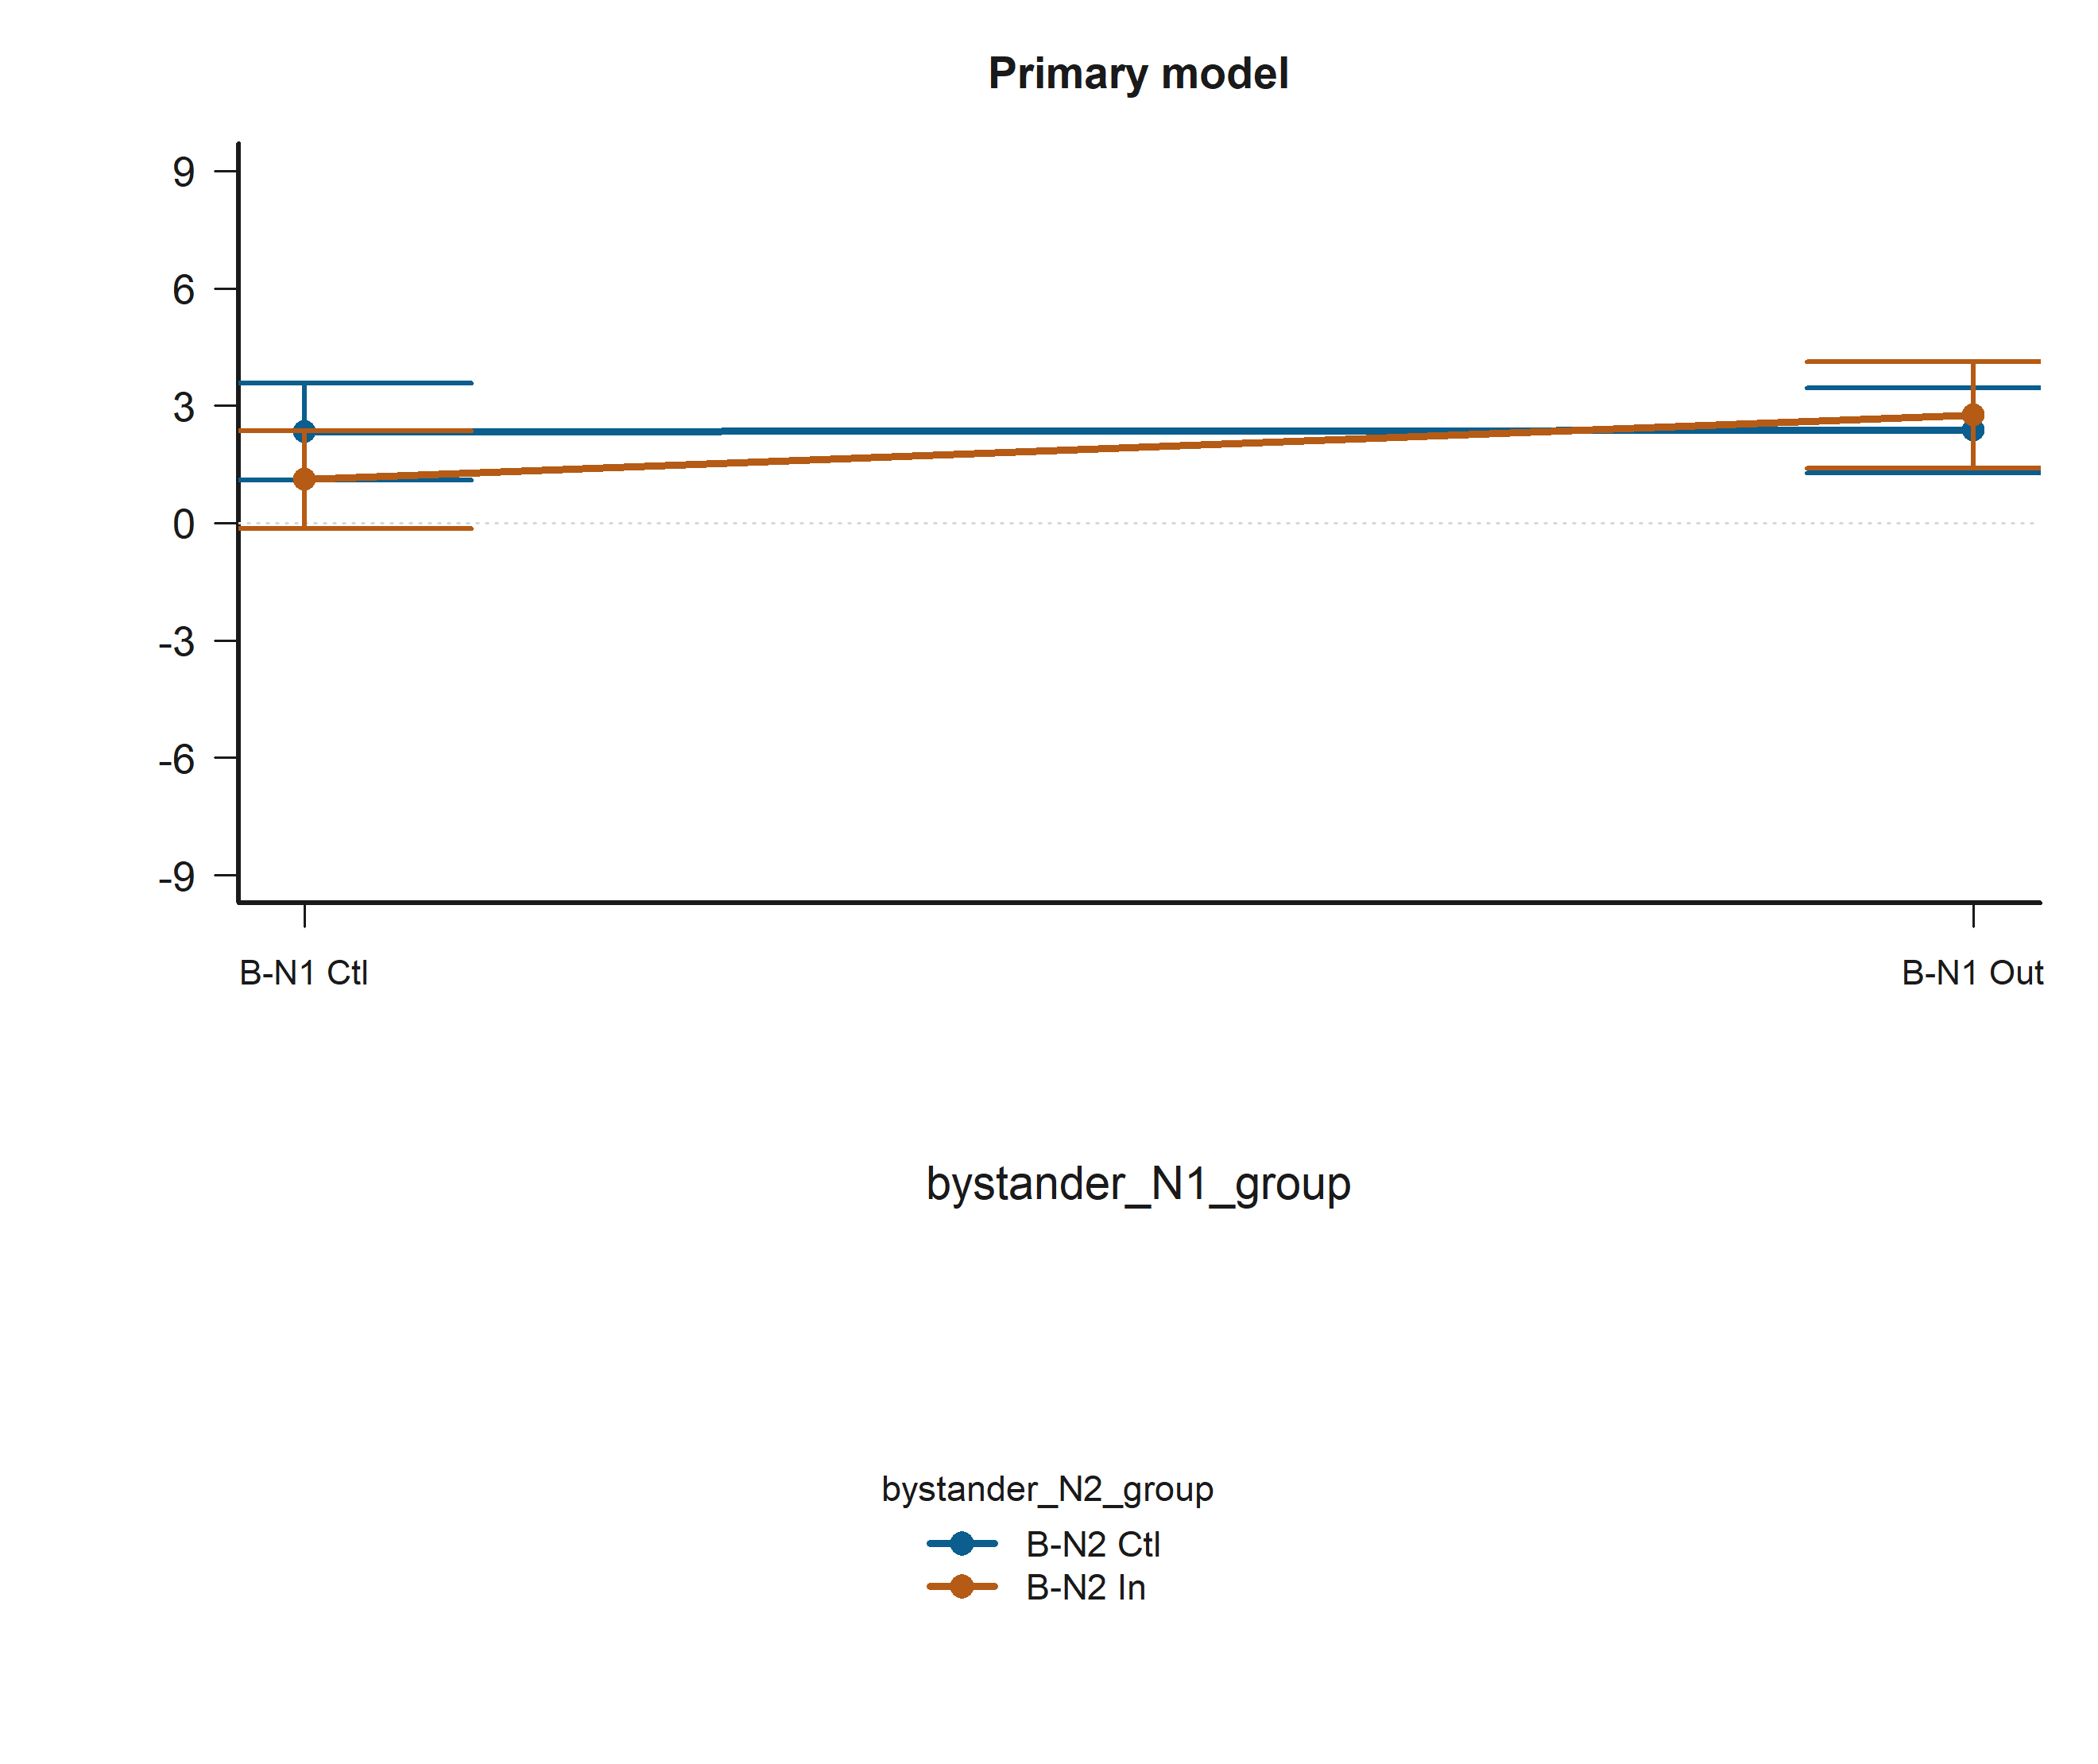
\includegraphics[width=0.92\textwidth]{../figures/figure_sig_all_judgments_bystander_bystander_n1_groupout_bystander_n2_groupin_judgments_bystander_bystander_n1_outgroup_ref_control_x_bystander_n2_ingroup_ref_control.png}
\caption{Interaction Plot for Bystander-N1: Outgroup (ref = Control) x Bystander-N2: Ingroup (ref = Control) in the judgments\_bystander. The panels show predicted judgments on the observed -9 to 9 scale with 95\% confidence intervals. Abbrev.: FS / EC / PT / PD = IRI subscales; N1 / N2 = negotiator 1 / negotiator 2; B-V = bystander-victim relation; V-N1 / V-N2 = victim-negotiator relations; B-N1 / B-N2 = bystander-negotiator relations; Vic / Obs = victim / observer subset; In / Out / Ctl = ingroup / outgroup / control label hidden; SameFac = N1 and N2 same faculty; SES = economic status.}
\label{fig:sig_all_judgments_bystander_bystander_n1_groupout_bystander_n2_groupin}
\end{figure}

Bystander-N1: Outgroup (ref = Control) is statistically significant in:
\begin{itemize}
  \item Empathy x Relational Status Model B (Tobit random-intercepts)
\end{itemize}
Figure \ref{fig:sig_all_judgments_bystander_bystander_n1_groupout} shows that predicted judgment is higher for B-N1 Out than for B-N1 Ctl.

\begin{figure}[H]
\centering
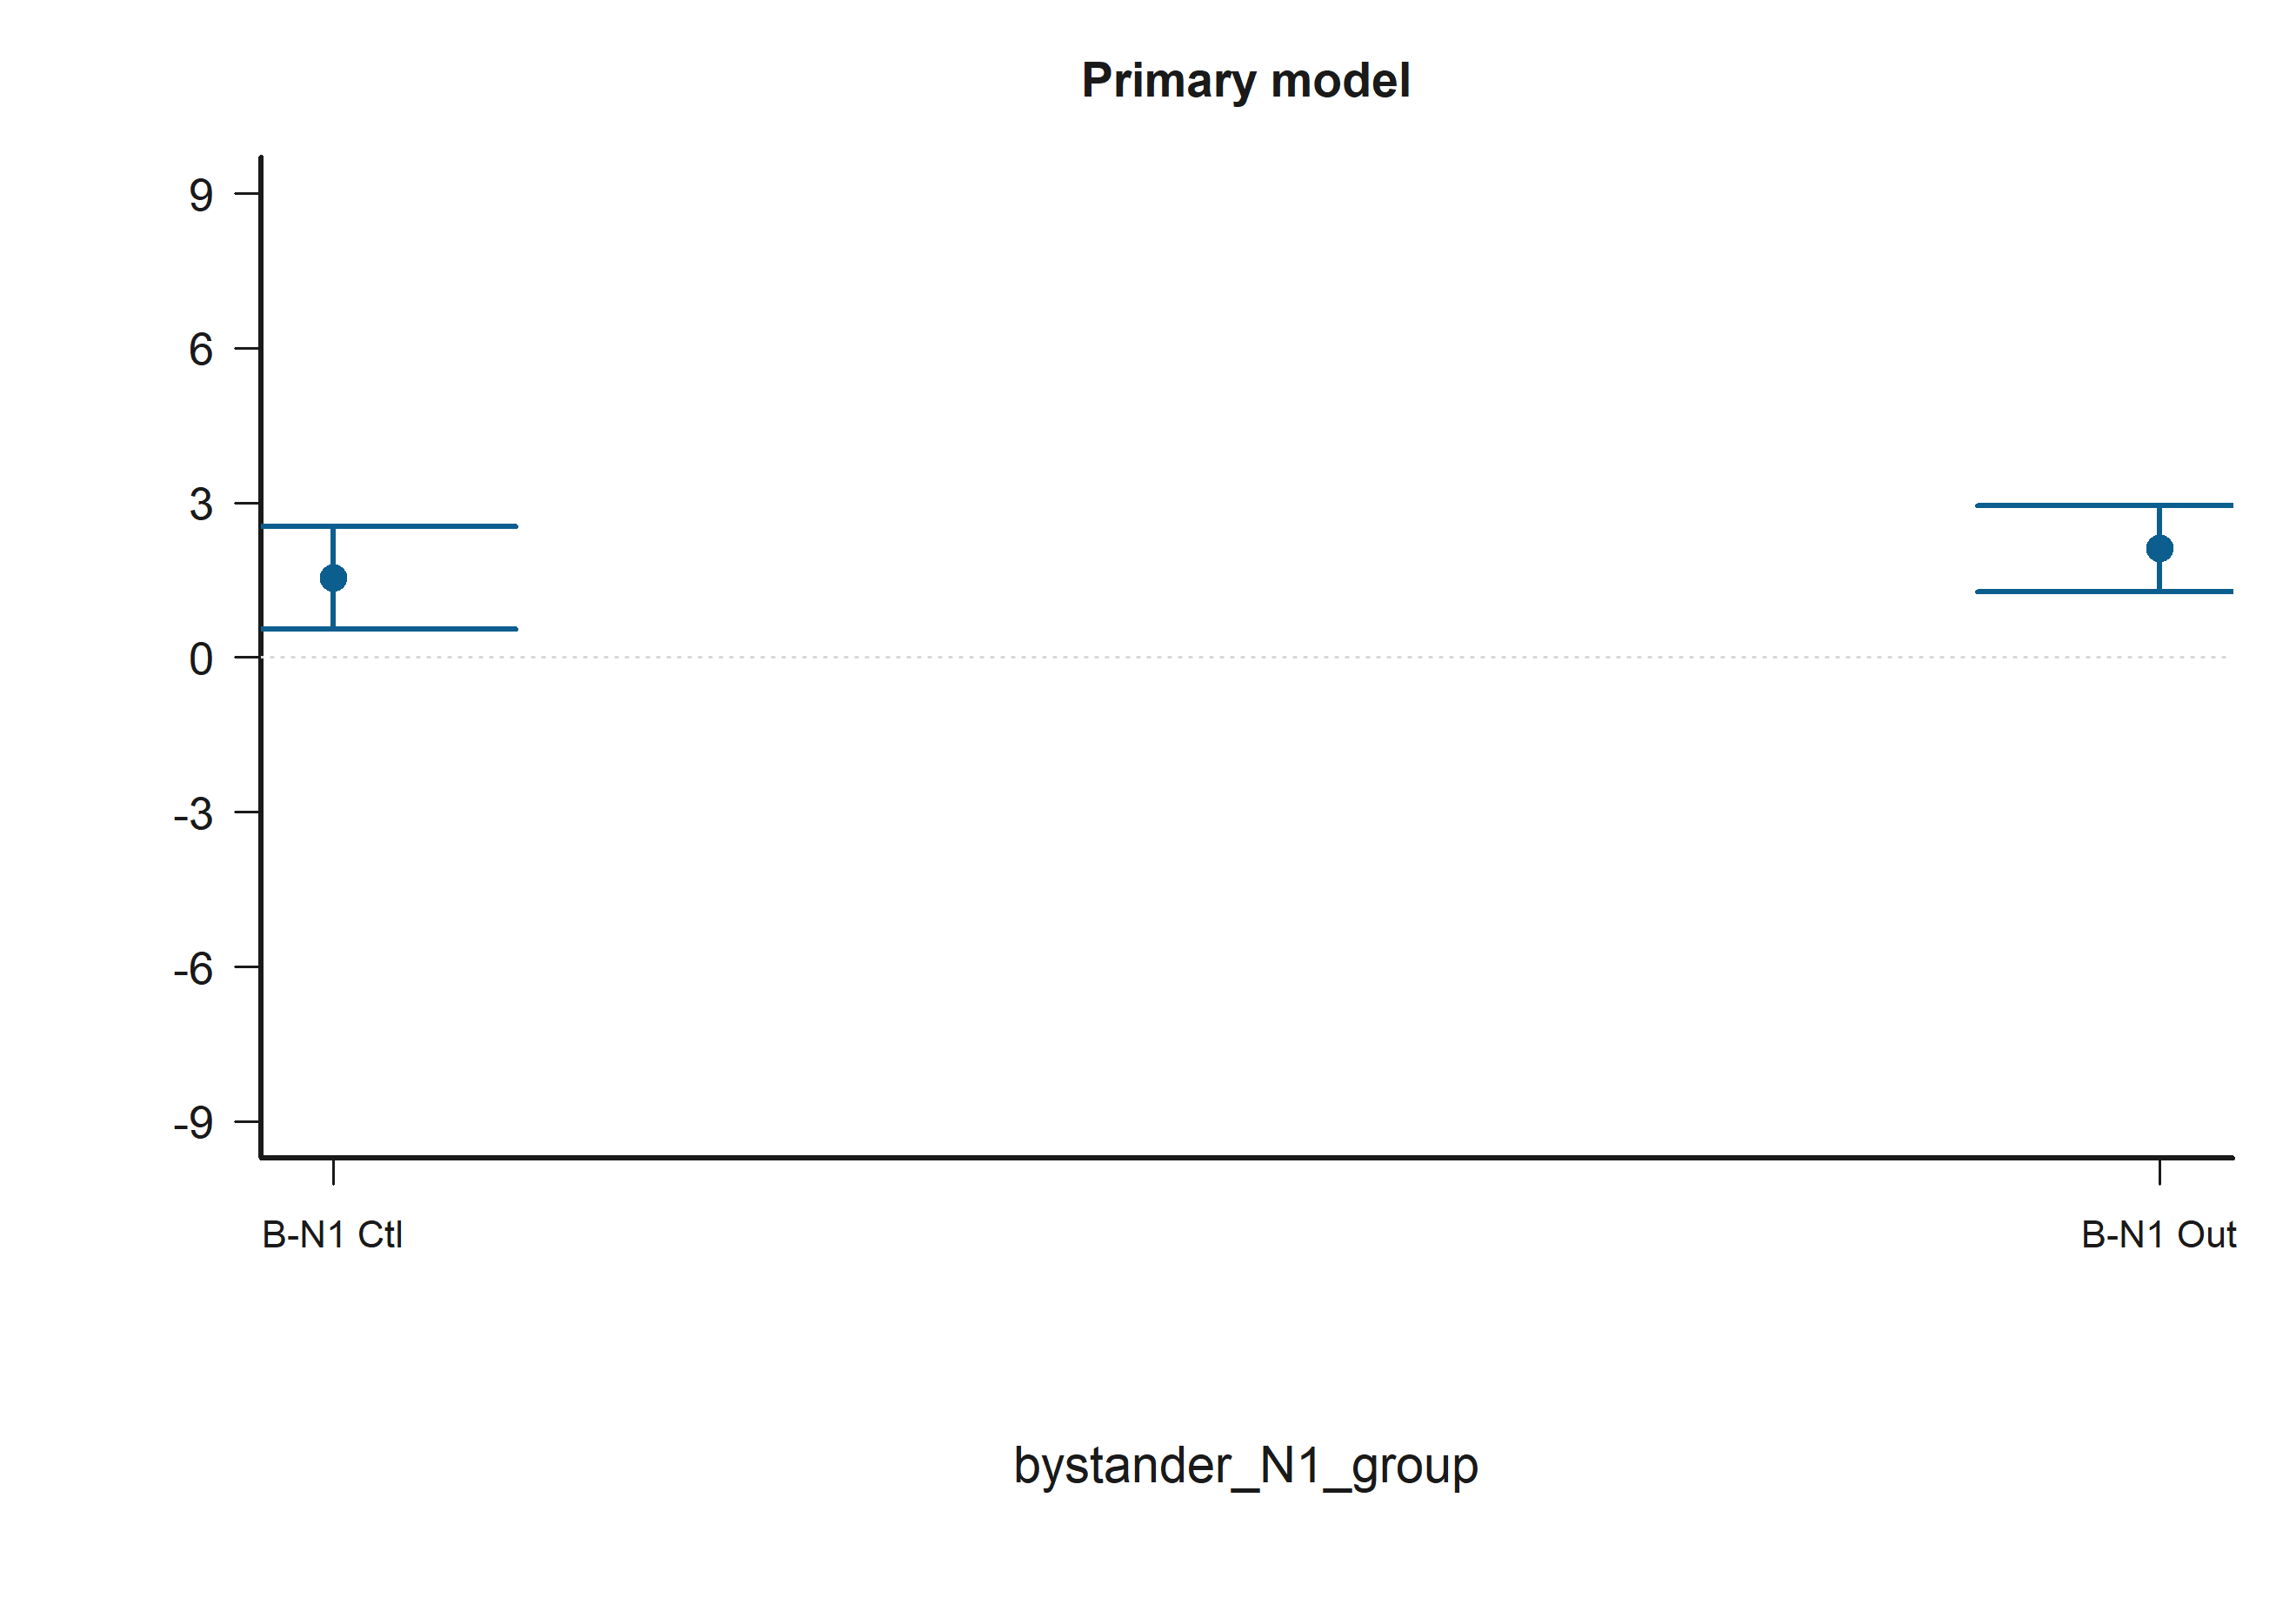
\includegraphics[width=0.92\textwidth]{../figures/figure_sig_all_judgments_bystander_bystander_n1_groupout_judgments_bystander_bystander_n1_outgroup_ref_control.png}
\caption{Grouped Prediction Plot for Bystander-N1: Outgroup (ref = Control) in the judgments\_bystander. The panels show predicted judgments on the observed -9 to 9 scale with 95\% confidence intervals. Abbrev.: FS / EC / PT / PD = IRI subscales; N1 / N2 = negotiator 1 / negotiator 2; B-V = bystander-victim relation; V-N1 / V-N2 = victim-negotiator relations; B-N1 / B-N2 = bystander-negotiator relations; Vic / Obs = victim / observer subset; In / Out / Ctl = ingroup / outgroup / control label hidden; SameFac = N1 and N2 same faculty; SES = economic status.}
\label{fig:sig_all_judgments_bystander_bystander_n1_groupout}
\end{figure}

Bystander-N1: Ingroup (ref = Control) x Bystander-N2: Ingroup (ref = Control) is statistically significant in:
\begin{itemize}
  \item Negotiator-Side Structure Model B (Tobit random-intercepts)
\end{itemize}
Figure \ref{fig:sig_all_judgments_bystander_bystander_n1_groupin_bystander_n2_groupin} shows that the predicted relationship rises most sharply for bystander\_N1\_group when the condition is B-N2 Ctl.

\begin{figure}[H]
\centering
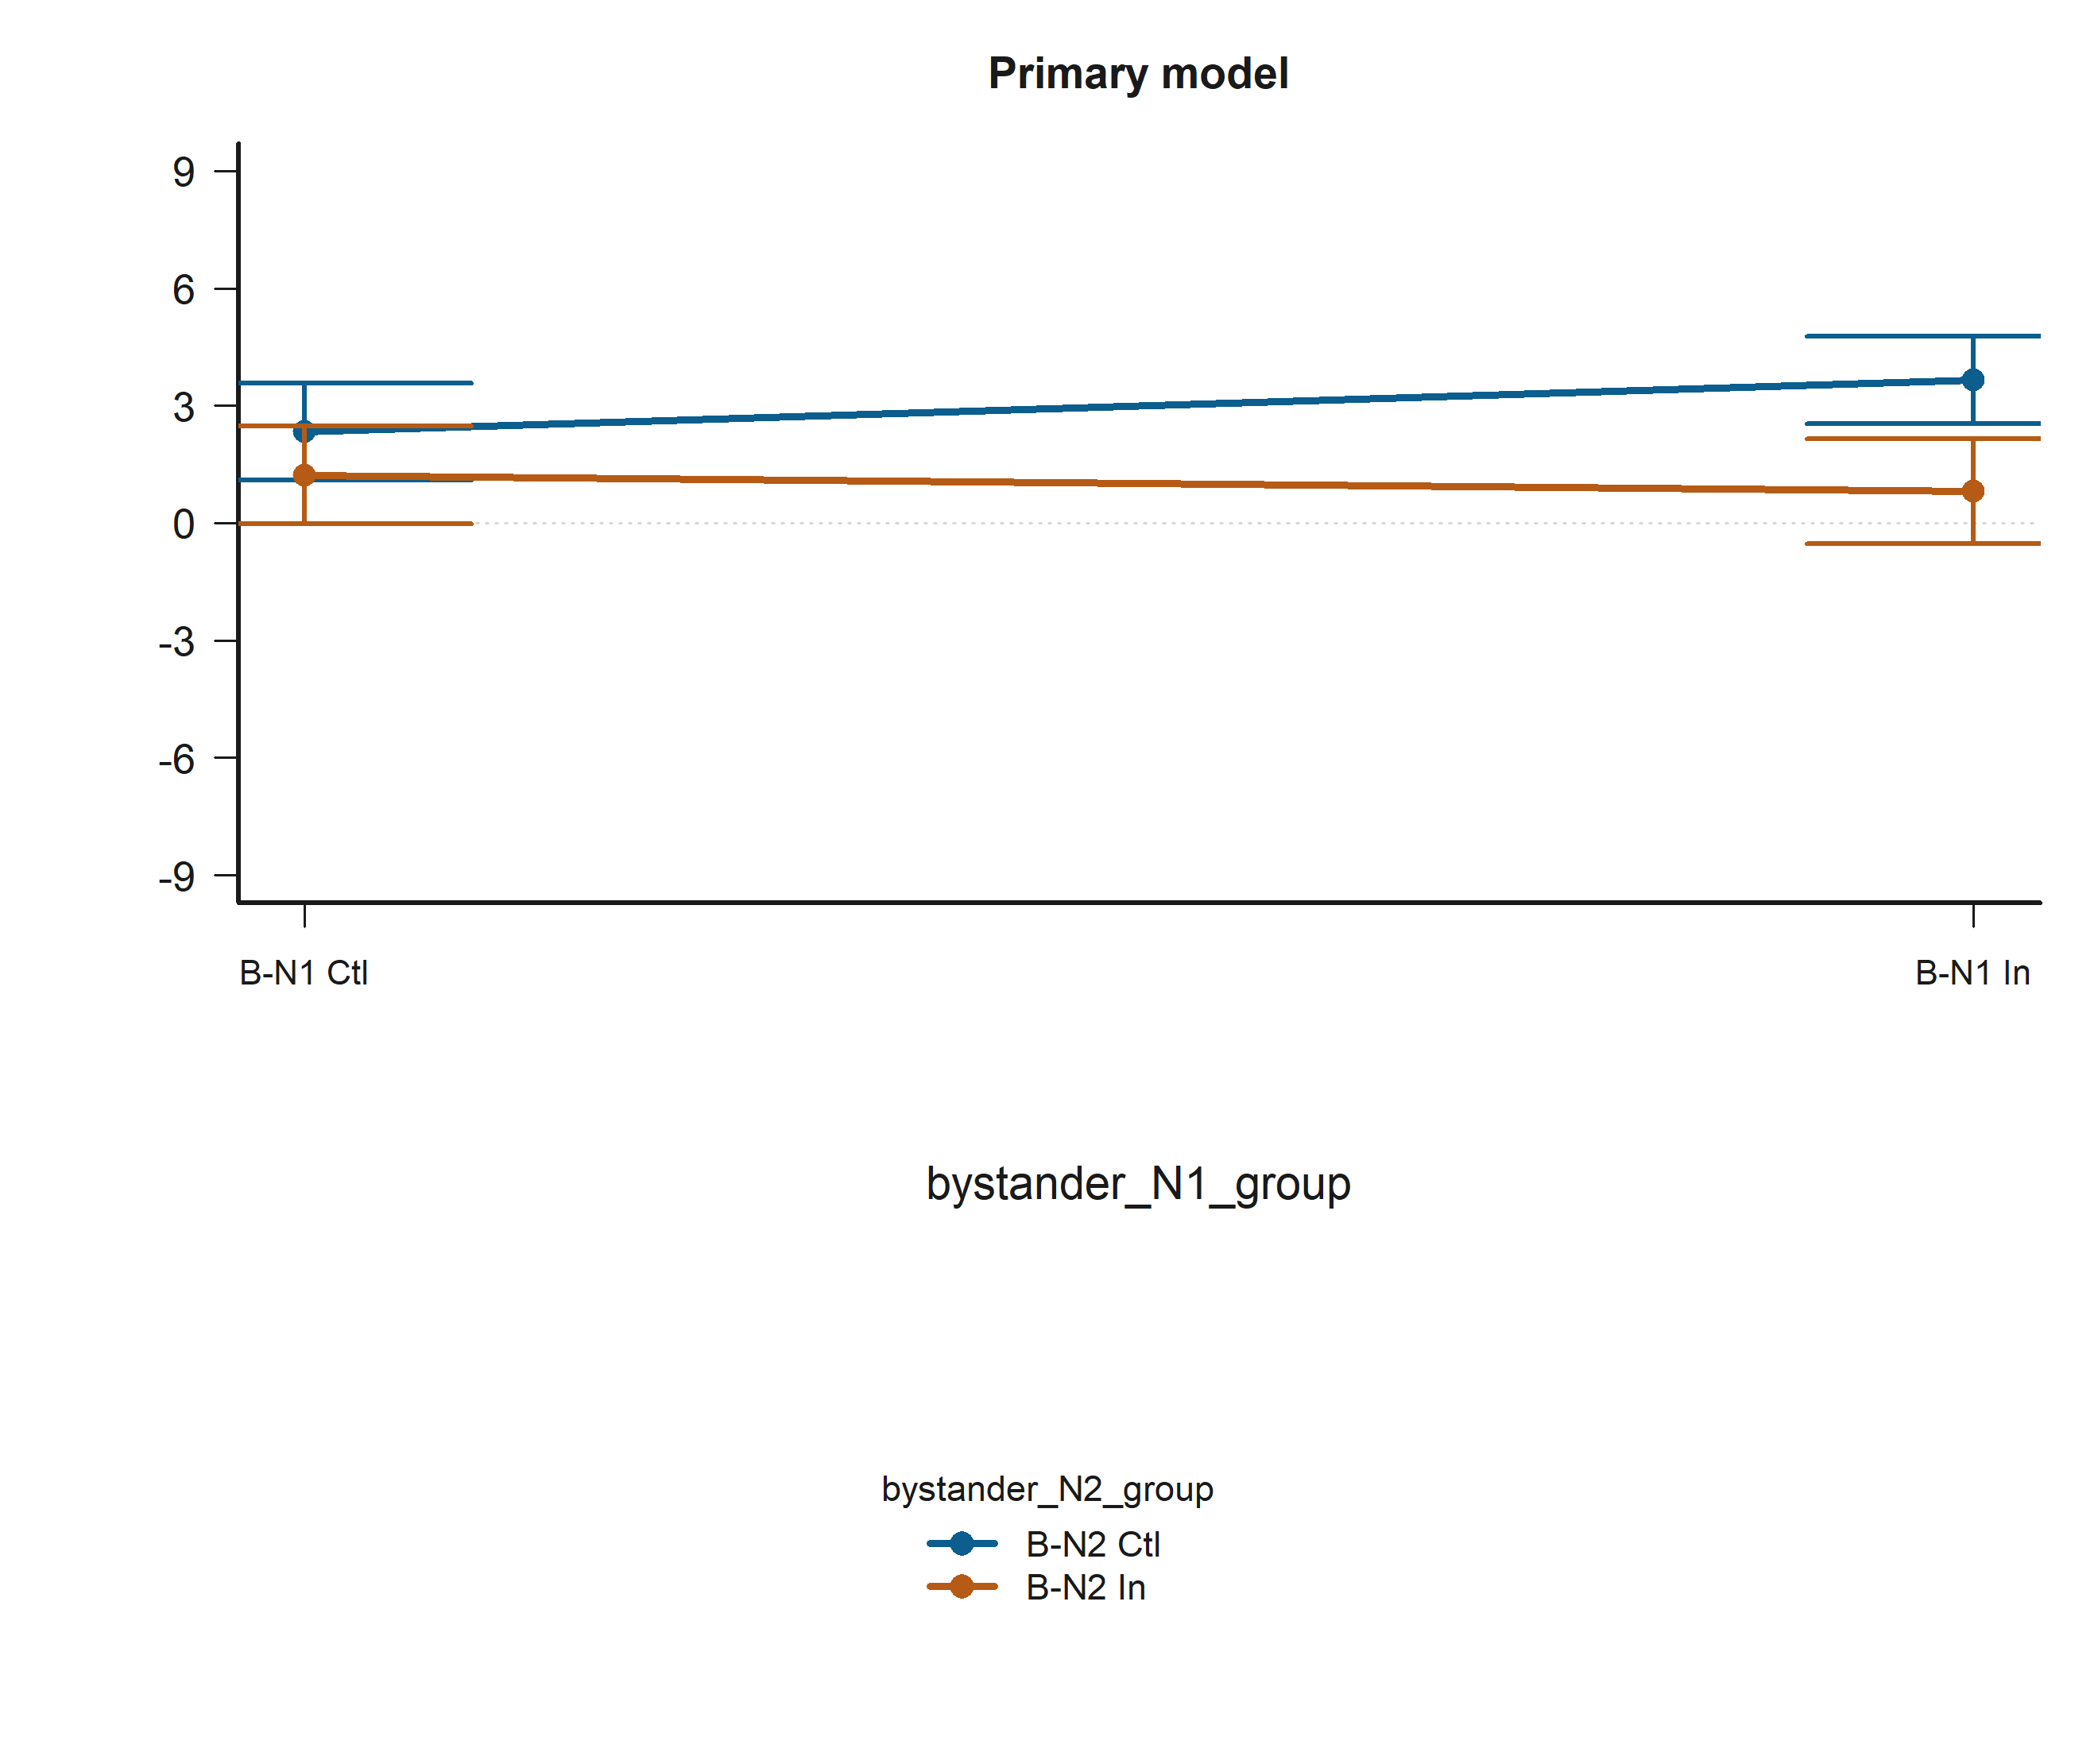
\includegraphics[width=0.92\textwidth]{../figures/figure_sig_all_judgments_bystander_bystander_n1_groupin_bystander_n2_groupin_judgments_bystander_bystander_n1_ingroup_ref_control_x_bystander_n2_ingroup_ref_control.png}
\caption{Interaction Plot for Bystander-N1: Ingroup (ref = Control) x Bystander-N2: Ingroup (ref = Control) in the judgments\_bystander. The panels show predicted judgments on the observed -9 to 9 scale with 95\% confidence intervals. Abbrev.: FS / EC / PT / PD = IRI subscales; N1 / N2 = negotiator 1 / negotiator 2; B-V = bystander-victim relation; V-N1 / V-N2 = victim-negotiator relations; B-N1 / B-N2 = bystander-negotiator relations; Vic / Obs = victim / observer subset; In / Out / Ctl = ingroup / outgroup / control label hidden; SameFac = N1 and N2 same faculty; SES = economic status.}
\label{fig:sig_all_judgments_bystander_bystander_n1_groupin_bystander_n2_groupin}
\end{figure}

\paragraph{judgments\_victim}

Empathy: Perspective taking x Victim-N1: Outgroup (ref = Control) is statistically significant in:
\begin{itemize}
  \item Empathy x Relational Status Model B (Tobit random-intercepts)
\end{itemize}
Figure \ref{fig:sig_all_judgments_victim_iri_pt_victim_n1_groupout} shows that the predicted relationship rises most sharply for Empathy: Perspective taking when the condition is V-N1 Out.

\begin{figure}[H]
\centering
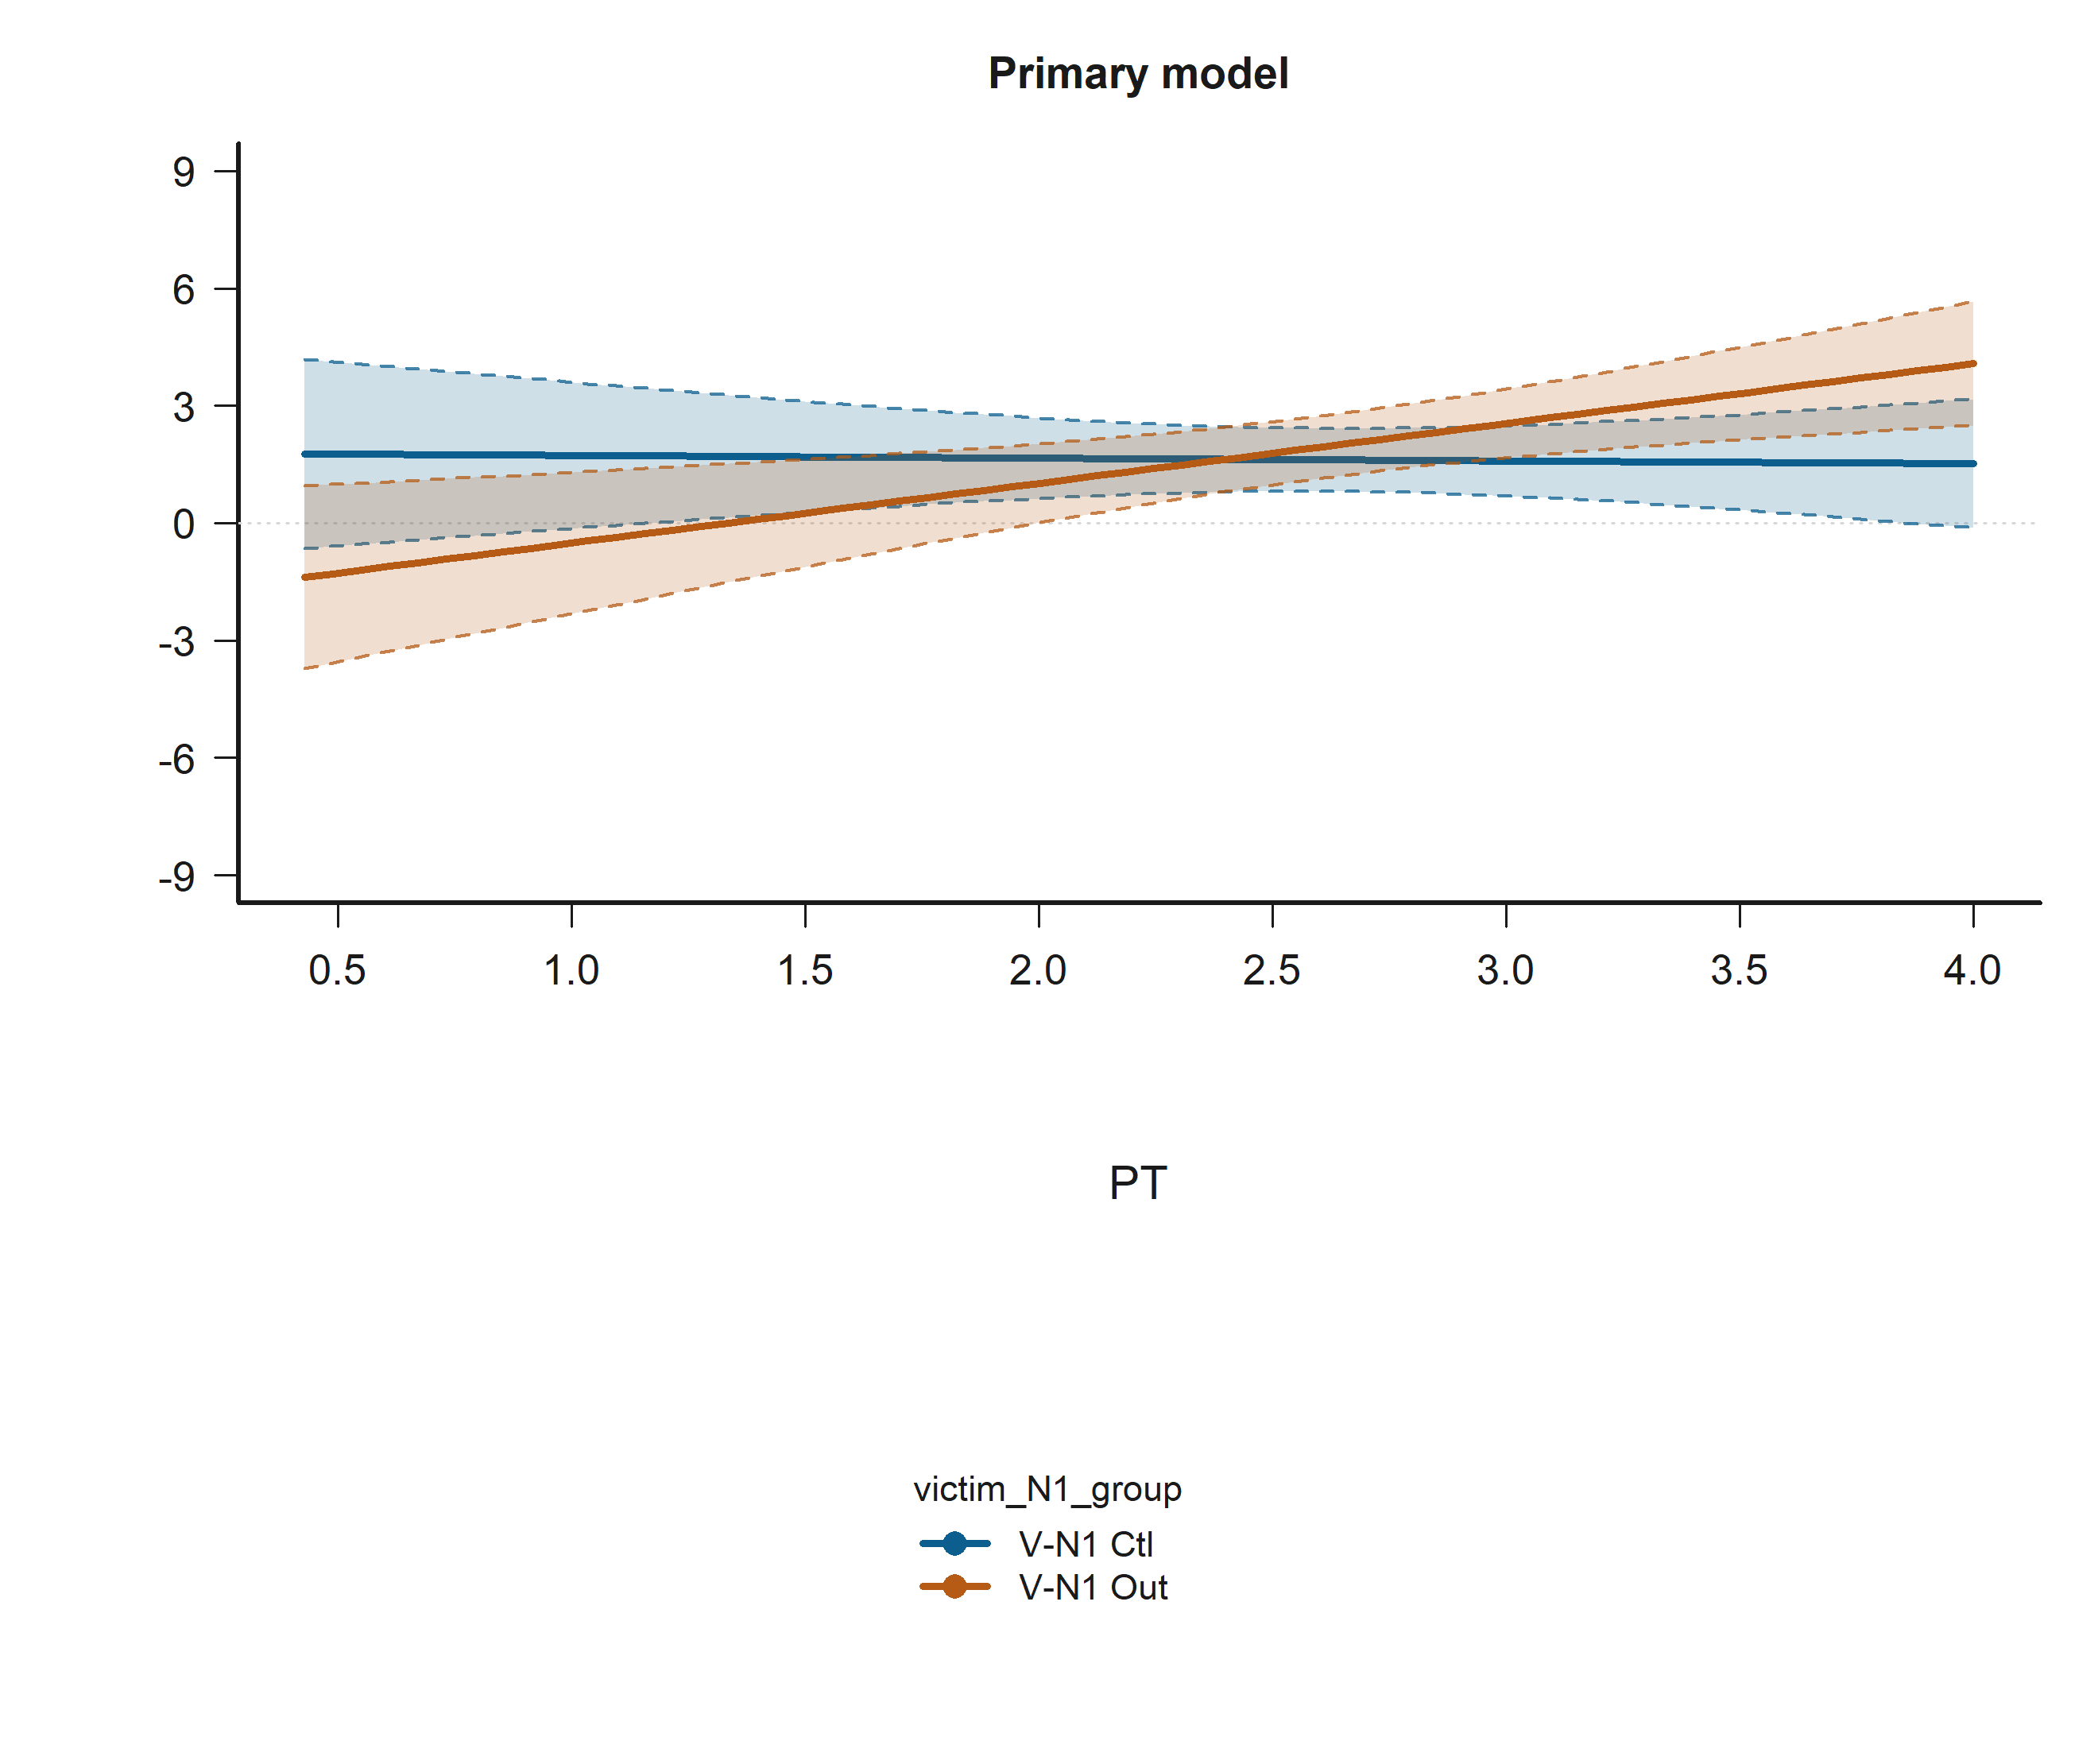
\includegraphics[width=0.92\textwidth]{../figures/figure_sig_all_judgments_victim_iri_pt_victim_n1_groupout_judgments_victim_empathy_perspective_taking_x_victim_n1_outgroup_ref_control.png}
\caption{Interaction Plot for Empathy: Perspective taking x Victim-N1: Outgroup (ref = Control) in the judgments\_victim. The panels show predicted judgments on the observed -9 to 9 scale with 95\% confidence intervals. Abbrev.: FS / EC / PT / PD = IRI subscales; N1 / N2 = negotiator 1 / negotiator 2; B-V = bystander-victim relation; V-N1 / V-N2 = victim-negotiator relations; B-N1 / B-N2 = bystander-negotiator relations; Vic / Obs = victim / observer subset; In / Out / Ctl = ingroup / outgroup / control label hidden; SameFac = N1 and N2 same faculty; SES = economic status.}
\label{fig:sig_all_judgments_victim_iri_pt_victim_n1_groupout}
\end{figure}

Empathy: Perspective taking is statistically significant in:
\begin{itemize}
  \item Empathy Effect Model B (Tobit random-intercepts)
  \item Negotiator-Side Structure Model B (Tobit random-intercepts)
\end{itemize}
Figure \ref{fig:sig_all_judgments_victim_iri_pt} shows that across the observed range, higher Empathy: Perspective taking corresponds to higher predicted judgment.

\begin{figure}[H]
\centering
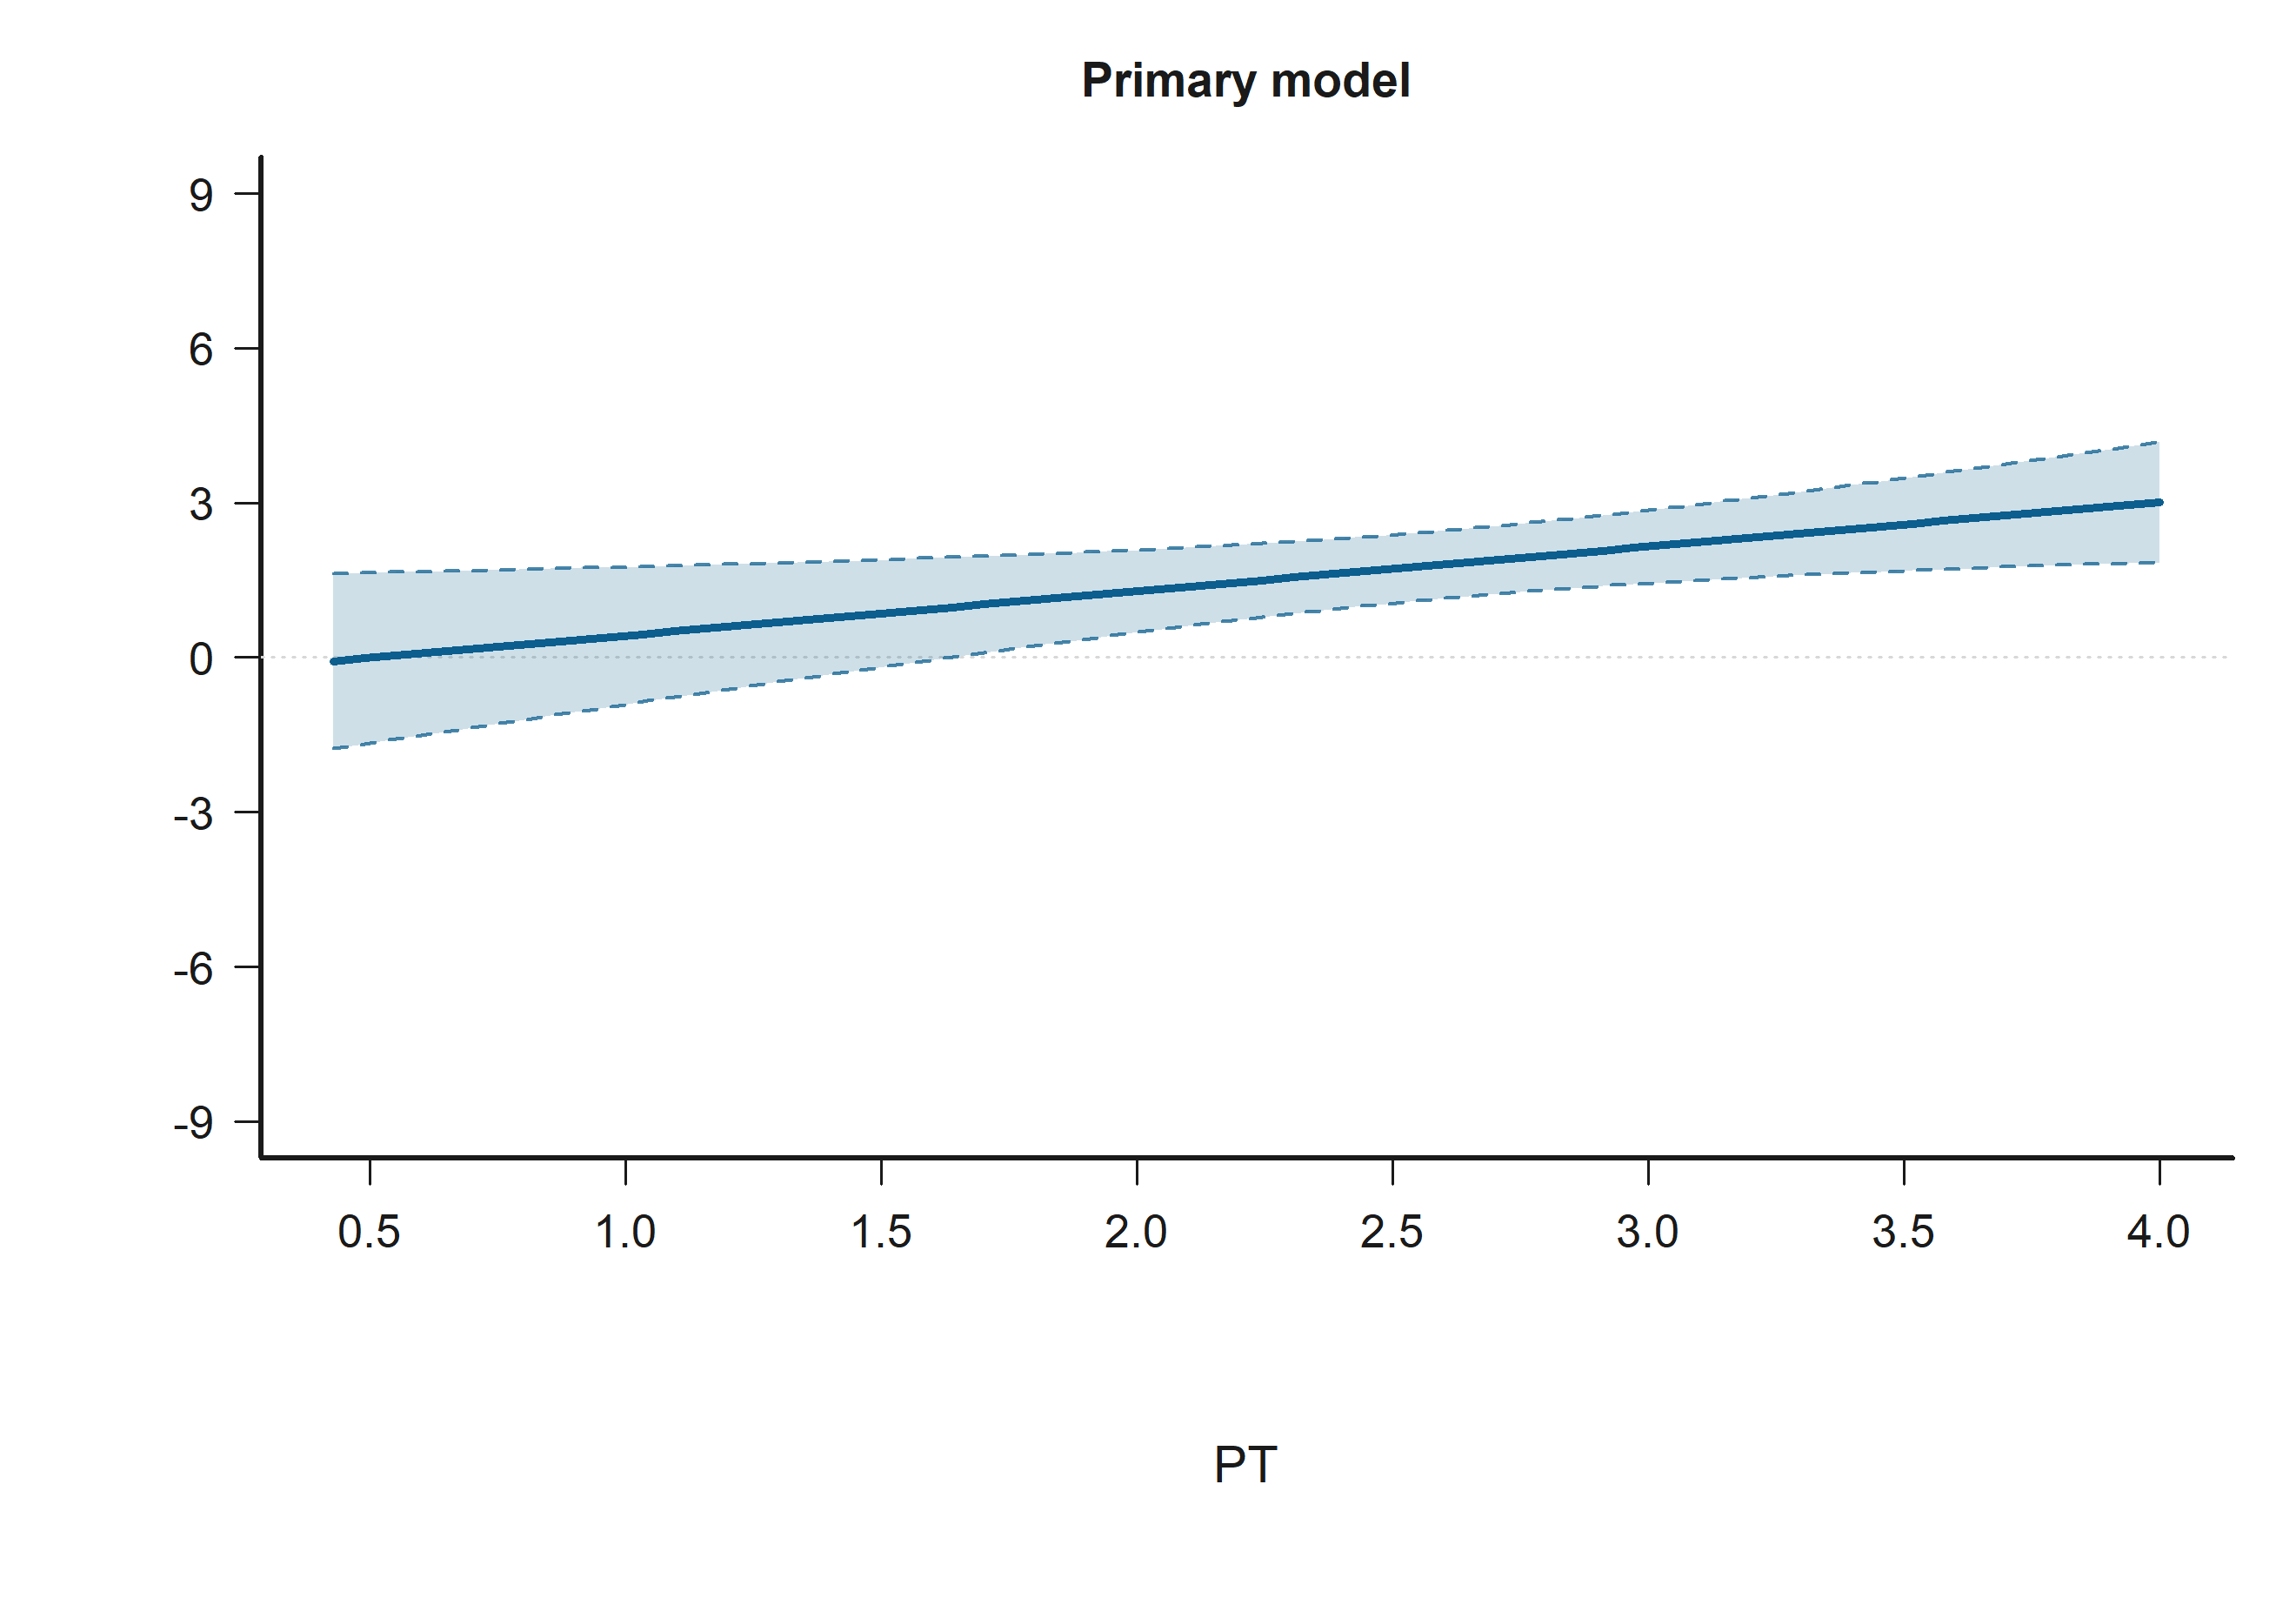
\includegraphics[width=0.92\textwidth]{../figures/figure_sig_all_judgments_victim_iri_pt_judgments_victim_empathy_perspective_taking.png}
\caption{Effect Plot for Empathy: Perspective taking in the judgments\_victim. The panels show predicted judgments on the observed -9 to 9 scale with 95\% confidence intervals. Abbrev.: FS / EC / PT / PD = IRI subscales; N1 / N2 = negotiator 1 / negotiator 2; B-V = bystander-victim relation; V-N1 / V-N2 = victim-negotiator relations; B-N1 / B-N2 = bystander-negotiator relations; Vic / Obs = victim / observer subset; In / Out / Ctl = ingroup / outgroup / control label hidden; SameFac = N1 and N2 same faculty; SES = economic status.}
\label{fig:sig_all_judgments_victim_iri_pt}
\end{figure}

Empathy: Empathic concern x Victim-N1: Outgroup (ref = Control) is statistically significant in:
\begin{itemize}
  \item Empathy x Relational Status Model B (Tobit random-intercepts)
\end{itemize}
Figure \ref{fig:sig_all_judgments_victim_iri_ec_victim_n1_groupout} shows that the predicted relationship falls most sharply for Empathy: Empathic concern when the condition is V-N1 Out.

\begin{figure}[H]
\centering
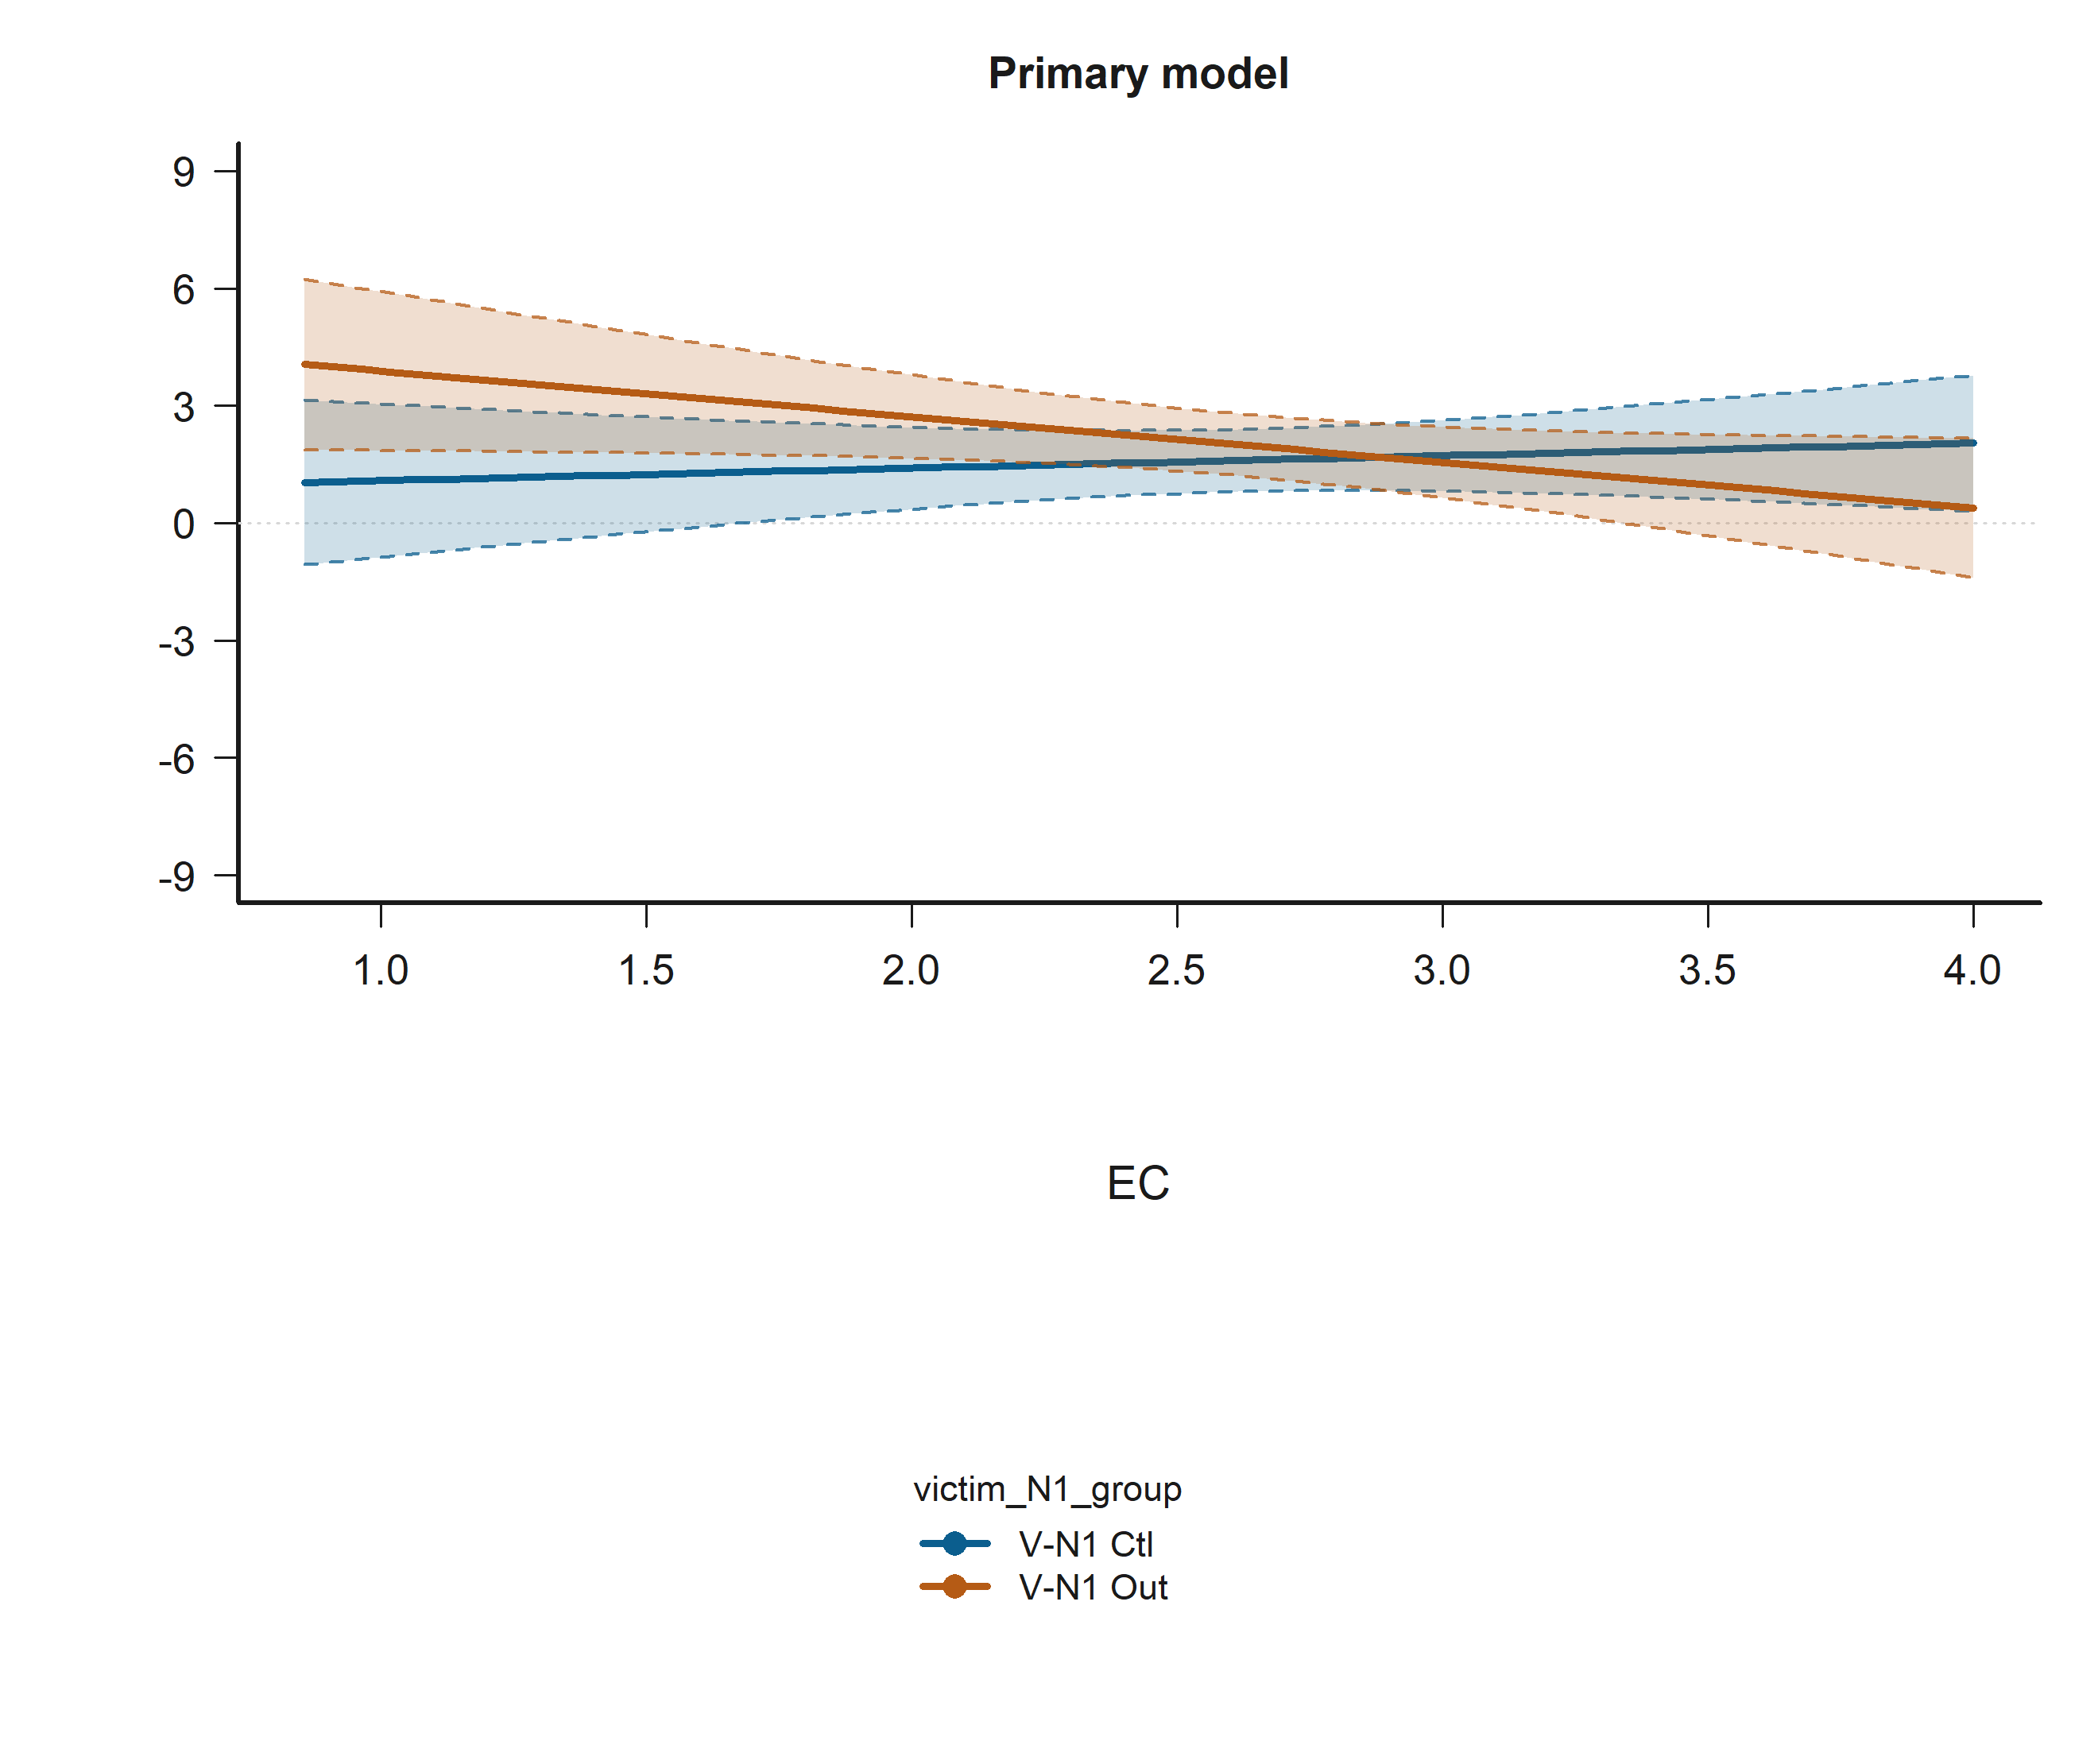
\includegraphics[width=0.92\textwidth]{../figures/figure_sig_all_judgments_victim_iri_ec_victim_n1_groupout_judgments_victim_empathy_empathic_concern_x_victim_n1_outgroup_ref_control.png}
\caption{Interaction Plot for Empathy: Empathic concern x Victim-N1: Outgroup (ref = Control) in the judgments\_victim. The panels show predicted judgments on the observed -9 to 9 scale with 95\% confidence intervals. Abbrev.: FS / EC / PT / PD = IRI subscales; N1 / N2 = negotiator 1 / negotiator 2; B-V = bystander-victim relation; V-N1 / V-N2 = victim-negotiator relations; B-N1 / B-N2 = bystander-negotiator relations; Vic / Obs = victim / observer subset; In / Out / Ctl = ingroup / outgroup / control label hidden; SameFac = N1 and N2 same faculty; SES = economic status.}
\label{fig:sig_all_judgments_victim_iri_ec_victim_n1_groupout}
\end{figure}

Engineering participant is statistically significant in:
\begin{itemize}
  \item Empathy x Relational Status Model B (Tobit random-intercepts)
  \item Empathy Effect Model B (Tobit random-intercepts)
  \item Negotiator-Side Structure Model B (Tobit random-intercepts)
\end{itemize}
Figure \ref{fig:sig_all_judgments_victim_participant_engineering} shows that predicted judgment is higher for Eng part. than for Hum part..

\begin{figure}[H]
\centering
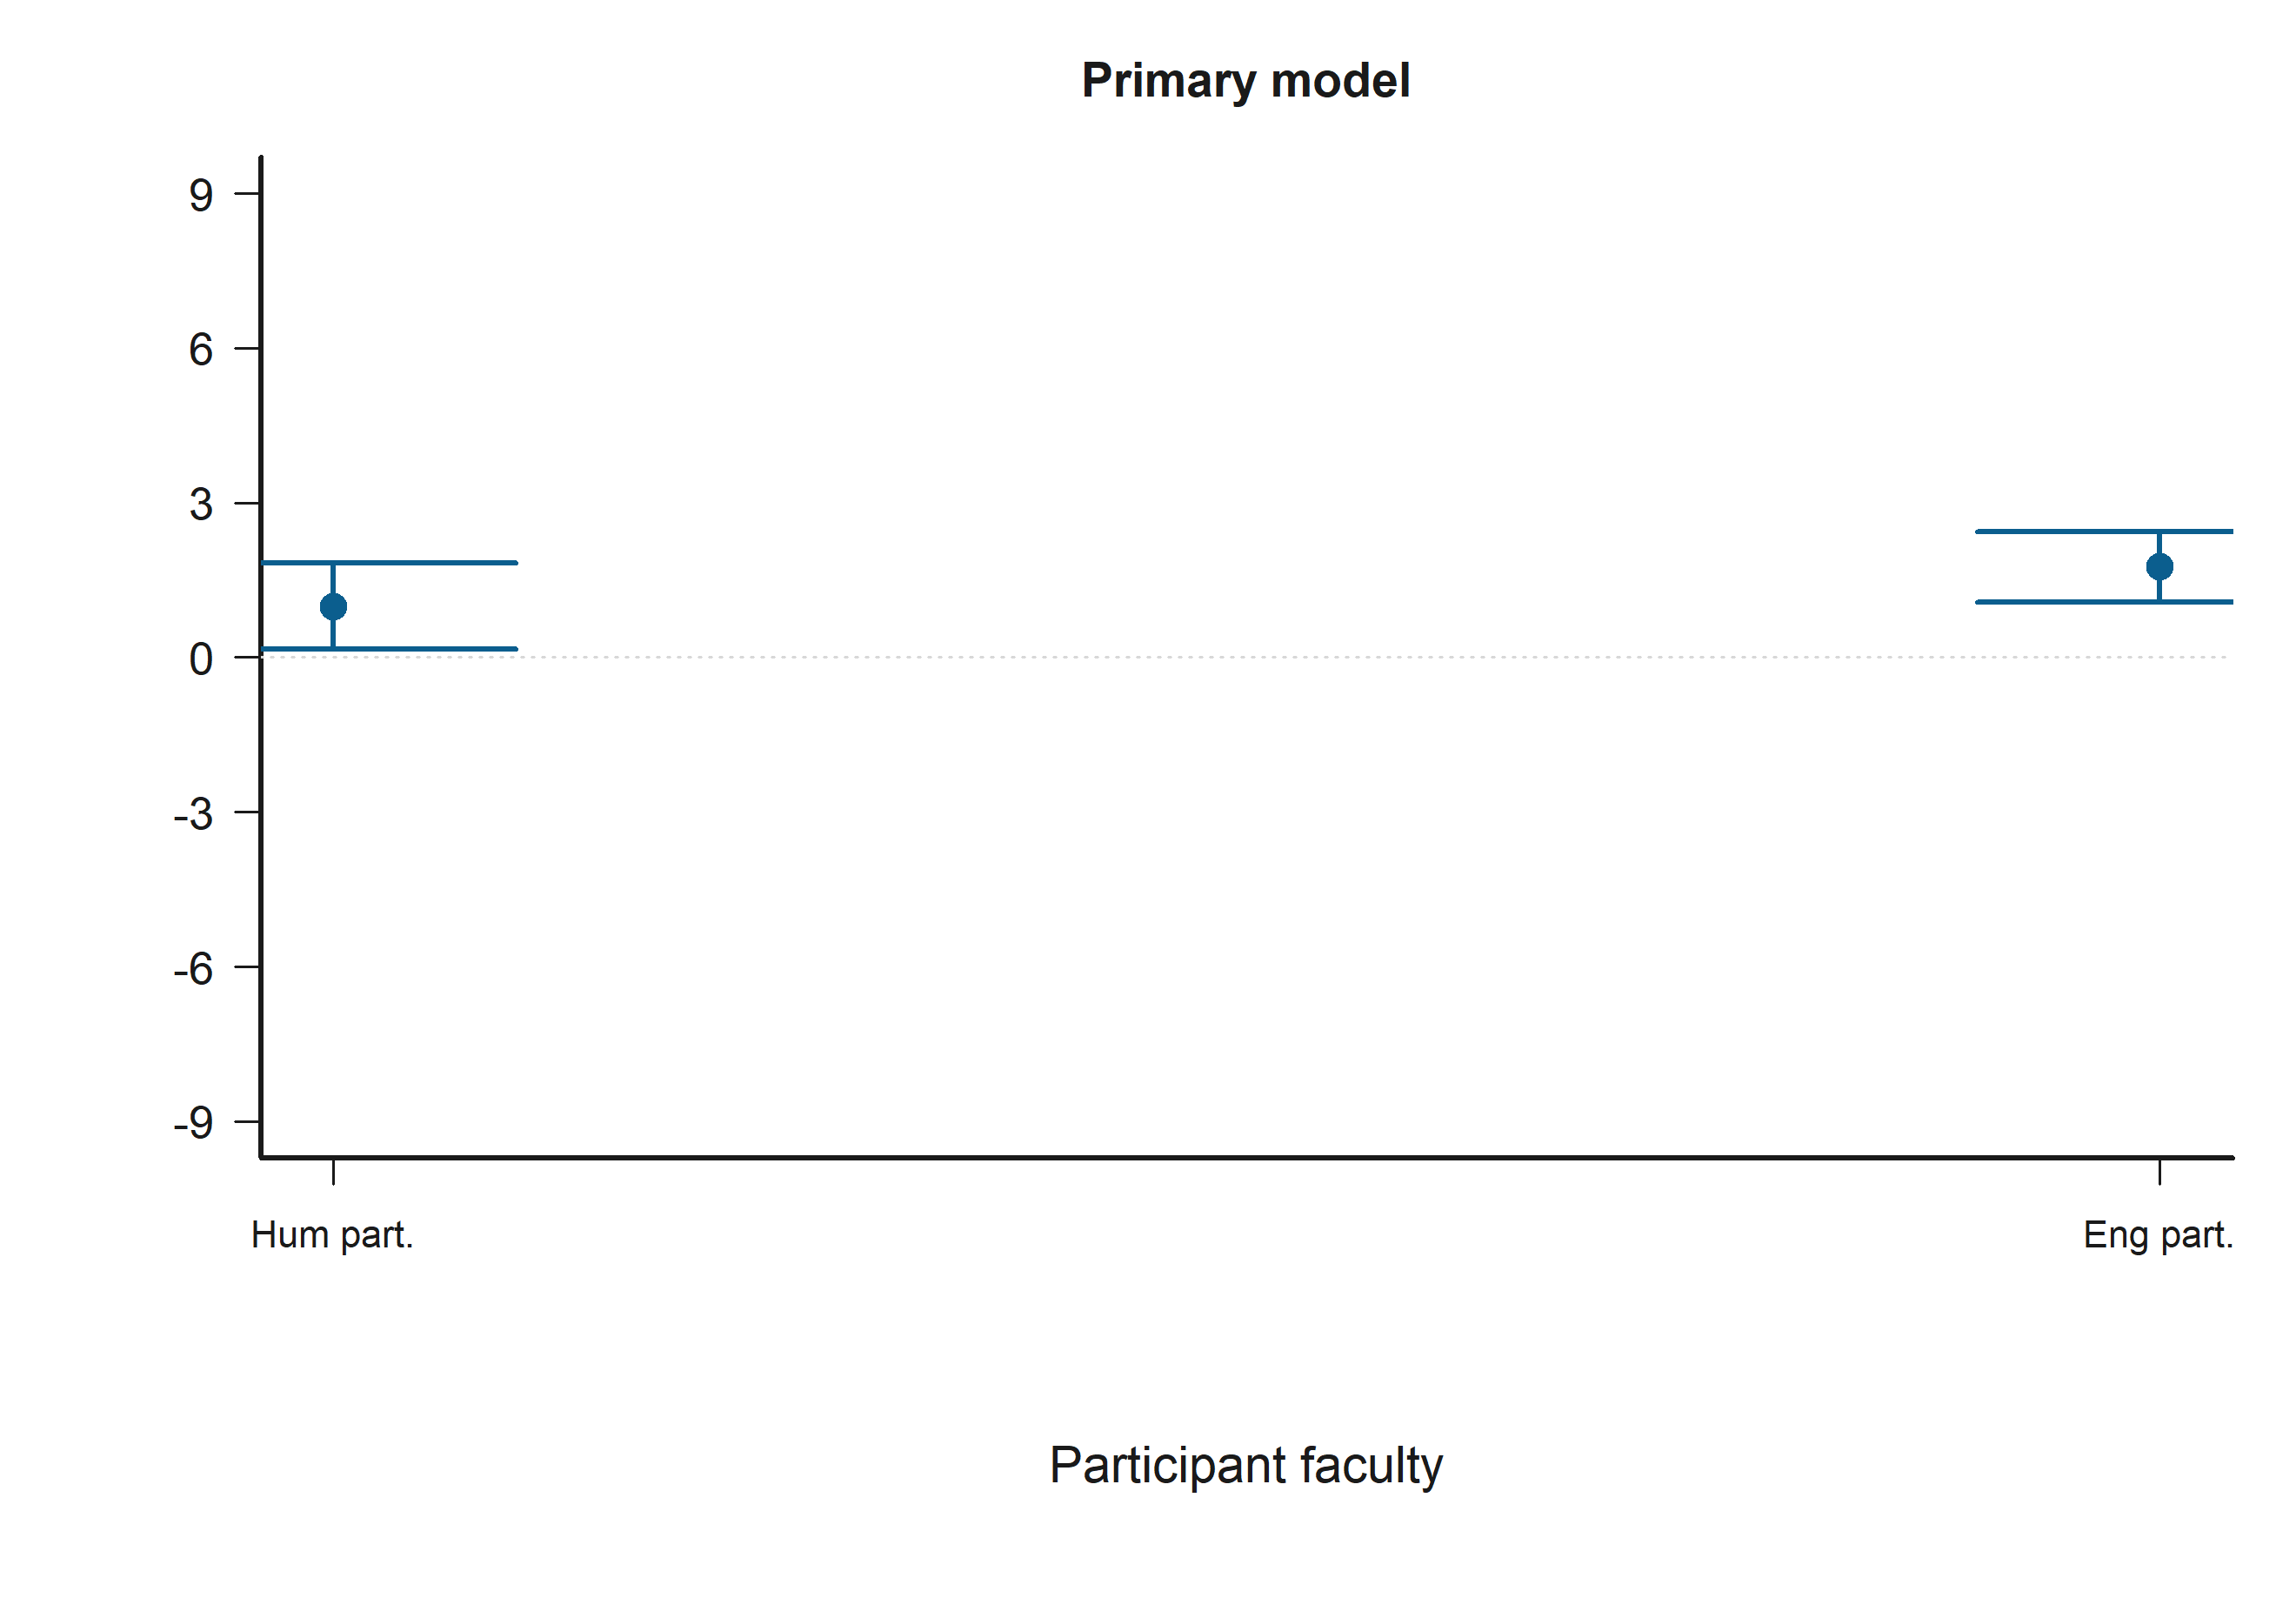
\includegraphics[width=0.92\textwidth]{../figures/figure_sig_all_judgments_victim_participant_engineering_judgments_victim_engineering_participant.png}
\caption{Grouped Prediction Plot for Engineering participant in the judgments\_victim. The panels show predicted judgments on the observed -9 to 9 scale with 95\% confidence intervals. Abbrev.: FS / EC / PT / PD = IRI subscales; N1 / N2 = negotiator 1 / negotiator 2; B-V = bystander-victim relation; V-N1 / V-N2 = victim-negotiator relations; B-N1 / B-N2 = bystander-negotiator relations; Vic / Obs = victim / observer subset; In / Out / Ctl = ingroup / outgroup / control label hidden; SameFac = N1 and N2 same faculty; SES = economic status.}
\label{fig:sig_all_judgments_victim_participant_engineering}
\end{figure}


\subsection{Integrated Hypothesis Conclusions}
The following summary restates each original hypothesis and indicates whether the available Tobit-random-intercepts estimates support it in the current data.
\begin{itemize}
\item H1. Original hypothesis: Empathy dimensions are associated with moral judgment severity after conditioning on role-specific N1/N2 relational predictors and the N1-N2 same-faculty context term. Victim subset: Tobit (random intercepts) conclusion: the available models point in the opposite direction of the hypothesis. Model B points in the opposite direction through Empathy: Perspective taking with a positive association (p = 0.017). Additional statistically significant signals include Empathy: Perspective taking with a positive association (p = 0.017) and Engineering participant with a positive association (p = 0.073). Bystander subset: Tobit (random intercepts) conclusion: the available models do not support the hypothesis. Model B does not support the hypothesis; none of four empathy dimensions are statistically significant, and the closest signal is Empathy: Empathic concern with a negative association (p = 0.144). Additional statistically significant signals include Age with a positive association (p = 0.002) and Bystander-N2: Ingroup (ref = Control) with a negative association (p = 0.054).
\item H2. Original hypothesis: Moral judgments vary with explicit N1/N2 relational structure and with the participant role. Bystander models retain participant-victim alignment and selective pairwise interactions. Victim subset: Tobit (random intercepts) conclusion: the available models do not support the hypothesis. Model B does not support the hypothesis; none of victim-side N1/N2 relational structure and interaction are statistically significant, and the closest signal is Victim-N1: Ingroup (ref = Control) x Victim-N2: Outgroup (ref = Control) with a positive association (p = 0.169). Additional statistically significant signals include Empathy: Perspective taking with a positive association (p = 0.019) and Engineering participant with a positive association (p = 0.073). Bystander subset: Tobit (random intercepts) conclusion: the available models support the hypothesis. Model B supports the hypothesis through Bystander-victim: Outgroup (ref = Ingroup) with a negative association (p = 0.035), Victim-N2: Ingroup (ref = Control) with a positive association (p = 0.071), Bystander-N2: Outgroup (ref = Control) with a negative association (p = 0.073), Bystander-N2: Ingroup (ref = Control) with a negative association (p = 0.083), and Bystander-N1: Ingroup (ref = Control) x Bystander-N2: Ingroup (ref = Control) with a negative association (p = 0.098). Additional statistically significant signals include Age with a positive association (p = 0.002) and Bystander-victim: Outgroup (ref = Ingroup) with a negative association (p = 0.035).
\item H3. Original hypothesis: The empathy effect depends on N1/N2 relational status indicators within each role-specific model while retaining relational controls and participant-level random intercepts. Victim subset: Tobit (random intercepts) conclusion: the available models support the hypothesis. Model B supports the hypothesis through Empathy: Perspective taking x Victim-N1: Outgroup (ref = Control) with a positive association (p = 0.014) and Empathy: Empathic concern x Victim-N1: Outgroup (ref = Control) with a negative association (p = 0.036). Additional statistically significant signals include Empathy: Perspective taking x Victim-N1: Outgroup (ref = Control) with a positive association (p = 0.014) and Empathy: Empathic concern x Victim-N1: Outgroup (ref = Control) with a negative association (p = 0.036). Bystander subset: Tobit (random intercepts) conclusion: the available models support the hypothesis. Model B supports the hypothesis through Bystander-N1: Outgroup (ref = Control) x Empathy: Fantasy scale with a negative association (p = 0.039), Bystander-victim: Outgroup (ref = Ingroup) x Empathy: Personal distress with a positive association (p = 0.064), and Bystander-N2: Outgroup (ref = Control) x Empathy: Perspective taking with a negative association (p = 0.084). Additional statistically significant signals include Age with a positive association (p = 0.002) and Bystander-N1: Outgroup (ref = Control) x Empathy: Fantasy scale with a negative association (p = 0.039).
\end{itemize}

\section{Hypothesis Validation and Results}
Detailed coefficient tables for each Tobit model with random intercepts, including predictor estimates, standard errors, p-values with conventional significance symbols, and estimator diagnostics for the victim and bystander subsets, are provided below.

\subsection{H1: Empathy Effect}
This section evaluates H1 separately in the victim and bystander subsets using the four IRI subscales as the active empathy specification: fantasy, empathic concern, perspective taking, and personal distress. The formula retains role-specific relational predictors for N1 and N2, the contextual same-faculty indicator between N1 and N2, and participant controls for sex, age, and economic status.
\subsubsection{Active Empathy-Construct Specification}
\textit{Model B subset-specific formulas.}
\begin{flushleft}
\textbf{Victim}
\[
\begin{aligned}
\texttt{judgement} &\sim iri\_fs + iri\_ec + iri\_pt + iri\_pd \\
&\quad + victim\_N1\_group + victim\_N2\_group + N1\_N2\_same\_faculty + participant\_engineering \\
&\quad + sex\_man + age + economic\_status
\end{aligned}
\]
\textbf{Bystander}
\[
\begin{aligned}
\texttt{judgement} &\sim iri\_fs + iri\_ec + iri\_pt + iri\_pd \\
&\quad + bystander\_victim\_group + bystander\_N1\_group + bystander\_N2\_group + victim\_N1\_group \\
&\quad + victim\_N2\_group + N1\_N2\_same\_faculty + participant\_engineering + sex\_man \\
&\quad + age + economic\_status
\end{aligned}
\]
\end{flushleft}

\paragraph{Victim subset}

\paragraph{Tobit estimator with random intercepts}

\begin{table}[H]
\centering
{\fontsize{11}{13}\selectfont
\renewcommand{\arraystretch}{1.10}
\caption{H1 active model: empathy-construct mixed-effects coefficients (Tobit estimator with random intercepts; Victim subset: 2,430 observations from 243 participants).}
\label{tab:h1_b_victim}
\begin{tabularx}{\textwidth}{>{\raggedright\arraybackslash}Xlll}
\toprule
Predictor & Estimate & Std. Error & p-value \\
\midrule
Base & -1.098 & 1.776 & 0.537 \\
FS & 0.420 & 0.268 & 0.117 \\
EC & -0.506 & 0.409 & 0.216 \\
PT & 0.864 & 0.362 & 0.017* \\
PD & -0.126 & 0.331 & 0.704 \\
V-N1 In & 0.076 & 0.352 & 0.830 \\
V-N1 Out & 0.363 & 0.355 & 0.307 \\
V-N2 In & 0.149 & 0.350 & 0.670 \\
V-N2 Out & -0.119 & 0.350 & 0.734 \\
SameFac & 0.292 & 0.306 & 0.341 \\
Eng part. & 0.733 & 0.408 & 0.073+ \\
Man & -0.199 & 0.423 & 0.639 \\
Age & -0.009 & 0.062 & 0.879 \\
SES & 0.287 & 0.189 & 0.129 \\
\bottomrule
\end{tabularx}
}
\end{table}
\begin{flushleft}
\footnotesize\textit{Note.} Estimator: Tobit estimator with random intercepts. Victim subset: 2,430 observations from 243 participants. Displayed predictors include FS, EC, PT, PD, V-N1 In, V-N1 Out, and 7 additional terms. Abbrev.: FS = fantasy; EC = empathic concern; PT = perspective taking; PD = personal distress; N1 = judged negotiator; N2 = counterpart negotiator; V-N1 = victim-negotiator 1 relation; V-N2 = victim-negotiator 2 relation; SameFac = N1 and N2 same faculty; SES = economic status.
\end{flushleft}

Interpretation:

Baseline judgment represents the starting moral score when all continuous variables are at their average and all group variables are at their reference levels (for active negotiator-status terms, the control-labeled condition). In this model, that baseline is estimated at -1.098 (p=0.537). The variable Empathy: Fantasy scale (the tendency to imaginatively get involved in fictitious stories (Fantasy subscale)) has an estimated effect of 0.420. The results show indicates little to no evidence of an effect, meaning the current data doesn't reliably show a relationship for this specific variable. For example, a 1-unit increase in this variable (or moving from the reference group to this group) would shift the moral judgment by approximately 0.42 points on the -9 to 9 scale. The variable Empathy: Empathic concern (the tendency to feel sympathy and compassion for others (Empathic Concern subscale)) has an estimated effect of -0.506. The results show indicates little to no evidence of an effect, meaning the current data doesn't reliably show a relationship for this specific variable. For example, a 1-unit increase in this variable (or moving from the reference group to this group) would shift the moral judgment by approximately -0.51 points on the -9 to 9 scale. The variable Empathy: Perspective taking (the tendency to look at things from another's point of view (Perspective Taking subscale)) has an estimated effect of 0.864. The results show indicates clear evidence of an effect, showing that this variable leads to an increase (higher scores) in the moral judgment. For example, a 1-unit increase in this variable (or moving from the reference group to this group) would shift the moral judgment by approximately 0.86 points on the -9 to 9 scale. The variable Empathy: Personal distress (the tendency to feel distress in uncomfortable social situations (Personal Distress subscale)) has an estimated effect of -0.126. The results show indicates little to no evidence of an effect, meaning the current data doesn't reliably show a relationship for this specific variable. For example, a 1-unit increase in this variable (or moving from the reference group to this group) would shift the moral judgment by approximately -0.13 points on the -9 to 9 scale. The variable Victim-N1: Ingroup (ref = Control) (whether N1 is ingroup to the victim (relative to the control-labeled baseline)) has an estimated effect of 0.076. The results show indicates little to no evidence of an effect, meaning the current data doesn't reliably show a relationship for this specific variable. For example, a 1-unit increase in this variable (or moving from the reference group to this group) would shift the moral judgment by approximately 0.08 points on the -9 to 9 scale. The variable Victim-N1: Outgroup (ref = Control) (whether N1 is outgroup to the victim (relative to the control-labeled baseline)) has an estimated effect of 0.363. The results show indicates little to no evidence of an effect, meaning the current data doesn't reliably show a relationship for this specific variable. For example, a 1-unit increase in this variable (or moving from the reference group to this group) would shift the moral judgment by approximately 0.36 points on the -9 to 9 scale. The variable Victim-N2: Ingroup (ref = Control) (whether N2 is ingroup to the victim (relative to the control-labeled baseline)) has an estimated effect of 0.149. The results show indicates little to no evidence of an effect, meaning the current data doesn't reliably show a relationship for this specific variable. For example, a 1-unit increase in this variable (or moving from the reference group to this group) would shift the moral judgment by approximately 0.15 points on the -9 to 9 scale. The variable Victim-N2: Outgroup (ref = Control) (whether N2 is outgroup to the victim (relative to the control-labeled baseline)) has an estimated effect of -0.119. The results show indicates little to no evidence of an effect, meaning the current data doesn't reliably show a relationship for this specific variable. For example, a 1-unit increase in this variable (or moving from the reference group to this group) would shift the moral judgment by approximately -0.12 points on the -9 to 9 scale. The variable N1 and N2 same faculty (whether N1 and N2 belong to the same faculty) has an estimated effect of 0.292. The results show indicates little to no evidence of an effect, meaning the current data doesn't reliably show a relationship for this specific variable. For example, a 1-unit increase in this variable (or moving from the reference group to this group) would shift the moral judgment by approximately 0.29 points on the -9 to 9 scale. The variable Engineering participant (whether the participant is from an Engineering faculty) has an estimated effect of 0.733. The results show indicates suggestive but inconclusive evidence of an effect, meaning the current data doesn't reliably show a relationship for this specific variable. For example, a 1-unit increase in this variable (or moving from the reference group to this group) would shift the moral judgment by approximately 0.73 points on the -9 to 9 scale. The variable Man participant (being a man (relative to being a woman)) has an estimated effect of -0.199. The results show indicates little to no evidence of an effect, meaning the current data doesn't reliably show a relationship for this specific variable. For example, a 1-unit increase in this variable (or moving from the reference group to this group) would shift the moral judgment by approximately -0.20 points on the -9 to 9 scale. The variable Age (the participant's age) has an estimated effect of -0.009. The results show indicates little to no evidence of an effect, meaning the current data doesn't reliably show a relationship for this specific variable. For example, a 1-unit increase in this variable (or moving from the reference group to this group) would shift the moral judgment by approximately -0.01 points on the -9 to 9 scale. The variable Economic status (the socioeconomic contextual stratum of the participant's background) has an estimated effect of 0.287. The results show indicates little to no evidence of an effect, meaning the current data doesn't reliably show a relationship for this specific variable. For example, a 1-unit increase in this variable (or moving from the reference group to this group) would shift the moral judgment by approximately 0.29 points on the -9 to 9 scale.

Diagnostics:

The Shapiro-Wilk test on the deviance residuals indicates a violation of the normality assumption (W = 0.949, p = 3.391e-28). The primary mixed-effects model retains participant-level random intercepts,.


\paragraph{Bystander subset}

\paragraph{Tobit estimator with random intercepts}

\begin{table}[H]
\centering
{\fontsize{11}{13}\selectfont
\renewcommand{\arraystretch}{1.10}
\caption{H1 active model: empathy-construct mixed-effects coefficients (Tobit estimator with random intercepts; Bystander subset: 2,430 observations from 243 participants).}
\label{tab:h1_b_bystander}
\begin{tabularx}{\textwidth}{>{\raggedright\arraybackslash}Xlll}
\toprule
Predictor & Estimate & Std. Error & p-value \\
\midrule
Base & -2.270 & 1.607 & 0.158 \\
FS & 0.095 & 0.242 & 0.696 \\
EC & -0.542 & 0.371 & 0.144 \\
PT & 0.381 & 0.327 & 0.244 \\
PD & 0.019 & 0.300 & 0.951 \\
B-V Out & -0.350 & 0.286 & 0.221 \\
B-N1 In & 0.653 & 0.396 & 0.099+ \\
B-N1 Out & 0.406 & 0.393 & 0.301 \\
B-N2 In & -0.760 & 0.394 & 0.054+ \\
B-N2 Out & -0.648 & 0.387 & 0.094+ \\
V-N1 In & -0.171 & 0.349 & 0.623 \\
V-N2 In & 0.576 & 0.350 & 0.100 \\
SameFac & 0.469 & 0.305 & 0.124 \\
Eng part. & 0.495 & 0.370 & 0.181 \\
Man & 0.516 & 0.383 & 0.178 \\
Age & 0.172 & 0.056 & 0.002** \\
SES & 0.089 & 0.171 & 0.602 \\
\bottomrule
\end{tabularx}
}
\end{table}
\begin{flushleft}
\footnotesize\textit{Note.} Estimator: Tobit estimator with random intercepts. Bystander subset: 2,430 observations from 243 participants. Displayed predictors include FS, EC, PT, PD, B-V Out, B-N1 In, and 10 additional terms. Abbrev.: FS = fantasy; EC = empathic concern; PT = perspective taking; PD = personal distress; N1 = judged negotiator; N2 = counterpart negotiator; B-V = bystander-victim relation; V-N1 = victim-negotiator 1 relation; V-N2 = victim-negotiator 2 relation; B-N1 = bystander-negotiator 1 relation; B-N2 = bystander-negotiator 2 relation; SameFac = N1 and N2 same faculty; SES = economic status.
\end{flushleft}

Interpretation:

Baseline judgment represents the starting moral score when all continuous variables are at their average and all group variables are at their reference levels (for active negotiator-status terms, the control-labeled condition). In this model, that baseline is estimated at -2.270 (p=0.158). The variable Empathy: Fantasy scale (the tendency to imaginatively get involved in fictitious stories (Fantasy subscale)) has an estimated effect of 0.095. The results show indicates little to no evidence of an effect, meaning the current data doesn't reliably show a relationship for this specific variable. For example, a 1-unit increase in this variable (or moving from the reference group to this group) would shift the moral judgment by approximately 0.09 points on the -9 to 9 scale. The variable Empathy: Empathic concern (the tendency to feel sympathy and compassion for others (Empathic Concern subscale)) has an estimated effect of -0.542. The results show indicates little to no evidence of an effect, meaning the current data doesn't reliably show a relationship for this specific variable. For example, a 1-unit increase in this variable (or moving from the reference group to this group) would shift the moral judgment by approximately -0.54 points on the -9 to 9 scale. The variable Empathy: Perspective taking (the tendency to look at things from another's point of view (Perspective Taking subscale)) has an estimated effect of 0.381. The results show indicates little to no evidence of an effect, meaning the current data doesn't reliably show a relationship for this specific variable. For example, a 1-unit increase in this variable (or moving from the reference group to this group) would shift the moral judgment by approximately 0.38 points on the -9 to 9 scale. The variable Empathy: Personal distress (the tendency to feel distress in uncomfortable social situations (Personal Distress subscale)) has an estimated effect of 0.019. The results show indicates little to no evidence of an effect, meaning the current data doesn't reliably show a relationship for this specific variable. For example, a 1-unit increase in this variable (or moving from the reference group to this group) would shift the moral judgment by approximately 0.02 points on the -9 to 9 scale. The variable Bystander-victim: Outgroup (ref = Ingroup) (whether the victim is outgroup to the bystander (reference = ingroup)) has an estimated effect of -0.350. The results show indicates little to no evidence of an effect, meaning the current data doesn't reliably show a relationship for this specific variable. For example, a 1-unit increase in this variable (or moving from the reference group to this group) would shift the moral judgment by approximately -0.35 points on the -9 to 9 scale. The variable Bystander-N1: Ingroup (ref = Control) (whether N1 is ingroup to the bystander (relative to the control-labeled baseline)) has an estimated effect of 0.653. The results show indicates suggestive but inconclusive evidence of an effect, meaning the current data doesn't reliably show a relationship for this specific variable. For example, a 1-unit increase in this variable (or moving from the reference group to this group) would shift the moral judgment by approximately 0.65 points on the -9 to 9 scale. The variable Bystander-N1: Outgroup (ref = Control) (whether N1 is outgroup to the bystander (relative to the control-labeled baseline)) has an estimated effect of 0.406. The results show indicates little to no evidence of an effect, meaning the current data doesn't reliably show a relationship for this specific variable. For example, a 1-unit increase in this variable (or moving from the reference group to this group) would shift the moral judgment by approximately 0.41 points on the -9 to 9 scale. The variable Bystander-N2: Ingroup (ref = Control) (whether N2 is ingroup to the bystander (relative to the control-labeled baseline)) has an estimated effect of -0.760. The results show indicates suggestive but inconclusive evidence of an effect, meaning the current data doesn't reliably show a relationship for this specific variable. For example, a 1-unit increase in this variable (or moving from the reference group to this group) would shift the moral judgment by approximately -0.76 points on the -9 to 9 scale. The variable Bystander-N2: Outgroup (ref = Control) (whether N2 is outgroup to the bystander (relative to the control-labeled baseline)) has an estimated effect of -0.648. The results show indicates suggestive but inconclusive evidence of an effect, meaning the current data doesn't reliably show a relationship for this specific variable. For example, a 1-unit increase in this variable (or moving from the reference group to this group) would shift the moral judgment by approximately -0.65 points on the -9 to 9 scale. The variable Victim-N1: Ingroup (ref = Control) (whether N1 is ingroup to the victim (relative to the control-labeled baseline)) has an estimated effect of -0.171. The results show indicates little to no evidence of an effect, meaning the current data doesn't reliably show a relationship for this specific variable. For example, a 1-unit increase in this variable (or moving from the reference group to this group) would shift the moral judgment by approximately -0.17 points on the -9 to 9 scale. The variable Victim-N2: Ingroup (ref = Control) (whether N2 is ingroup to the victim (relative to the control-labeled baseline)) has an estimated effect of 0.576. The results show indicates little to no evidence of an effect, meaning the current data doesn't reliably show a relationship for this specific variable. For example, a 1-unit increase in this variable (or moving from the reference group to this group) would shift the moral judgment by approximately 0.58 points on the -9 to 9 scale. The variable N1 and N2 same faculty (whether N1 and N2 belong to the same faculty) has an estimated effect of 0.469. The results show indicates little to no evidence of an effect, meaning the current data doesn't reliably show a relationship for this specific variable. For example, a 1-unit increase in this variable (or moving from the reference group to this group) would shift the moral judgment by approximately 0.47 points on the -9 to 9 scale. The variable Engineering participant (whether the participant is from an Engineering faculty) has an estimated effect of 0.495. The results show indicates little to no evidence of an effect, meaning the current data doesn't reliably show a relationship for this specific variable. For example, a 1-unit increase in this variable (or moving from the reference group to this group) would shift the moral judgment by approximately 0.49 points on the -9 to 9 scale. The variable Man participant (being a man (relative to being a woman)) has an estimated effect of 0.516. The results show indicates little to no evidence of an effect, meaning the current data doesn't reliably show a relationship for this specific variable. For example, a 1-unit increase in this variable (or moving from the reference group to this group) would shift the moral judgment by approximately 0.52 points on the -9 to 9 scale. The variable Age (the participant's age) has an estimated effect of 0.172. The results show indicates strong evidence of an effect, showing that this variable leads to an increase (higher scores) in the moral judgment. For example, a 1-unit increase in this variable (or moving from the reference group to this group) would shift the moral judgment by approximately 0.17 points on the -9 to 9 scale. The variable Economic status (the socioeconomic contextual stratum of the participant's background) has an estimated effect of 0.089. The results show indicates little to no evidence of an effect, meaning the current data doesn't reliably show a relationship for this specific variable. For example, a 1-unit increase in this variable (or moving from the reference group to this group) would shift the moral judgment by approximately 0.09 points on the -9 to 9 scale.

Diagnostics:

The Shapiro-Wilk test on the deviance residuals indicates a violation of the normality assumption (W = 0.968, p = 1.006e-22). The primary mixed-effects model retains participant-level random intercepts,.



\subsection{H2: Negotiator-Side Relational Structure}
This section estimates H2 separately in the victim and bystander subsets. In the victim subset, H2 evaluates the joint victim-N1 and victim-N2 structure through their interaction, while retaining the N1-N2 same-faculty context term. In the bystander subset, H2 retains bystander-victim alignment, bystander-victim x bystander-N1/N2 interactions, selective N1-by-N2 and victim-by-negotiator interaction blocks, and N1-N2 same-faculty as a contextual main effect.
\textbf{Victim-subset H2}
\[
\begin{aligned}
y_{isj,\mathrm{Victim}} &= \beta_0 + \beta_1\,\mathrm{Empathy}_i + \gamma_1\,\mathrm{Victim\text{-}N1}_{isj} + \gamma_2\,\mathrm{Victim\text{-}N2}_{isj} \\
&\quad +\ \gamma_3\,(\mathrm{Victim\text{-}N1}_{isj}\times\mathrm{Victim\text{-}N2}_{isj}) + \gamma_4\,\mathrm{SameFac}_{isj} + \boldsymbol{\delta}'\mathbf{Z}_i \\
&\quad +\ u_i + v_{\mathrm{case}(i,s,j)} + \epsilon_{isj} \\
\end{aligned}
\]

\textbf{Bystander-subset H2}
\[
\begin{aligned}
y_{isj,\mathrm{Obs}} &= \beta_0 + \beta_1\,\mathrm{Empathy}_i + \eta\,\mathrm{Bystander\text{-}Victim}_{isj} \\
&\quad +\ \boldsymbol{\kappa}'\bigl(\mathrm{Bystander\text{-}Victim}_{isj}\times\mathrm{Bystander\text{-}N}_{isj}\bigr) + \boldsymbol{\gamma}'\mathbf{R}_{isj} \\
&\quad +\ \boldsymbol{\delta}'\mathbf{Z}_i + u_i + v_{\mathrm{case}(i,s,j)} + \epsilon_{isj} \\
\end{aligned}
\]

\subsubsection{Active Empathy-Construct Specification}
\textit{Model B subset-specific formulas.}
\begin{flushleft}
\textbf{Victim}
\[
\begin{aligned}
\texttt{judgement} &\sim iri\_fs + iri\_ec + iri\_pt + iri\_pd \\
&\quad + victim\_N1\_group * victim\_N2\_group + N1\_N2\_same\_faculty + participant\_engineering + sex\_man \\
&\quad + age + economic\_status
\end{aligned}
\]
\textbf{Bystander}
\[
\begin{aligned}
\texttt{judgement} &\sim iri\_fs + iri\_ec + iri\_pt + iri\_pd \\
&\quad + bystander\_victim\_group + bystander\_N1\_group * bystander\_N2\_group + bystander\_victim\_group:bystander\_N1\_group + bystander\_victim\_group:bystander\_N2\_group \\
&\quad + victim\_N1\_group * victim\_N2\_group + N1\_N2\_same\_faculty + participant\_engineering + sex\_man \\
&\quad + age + economic\_status
\end{aligned}
\]
\end{flushleft}

\paragraph{Victim subset}

\paragraph{Tobit estimator with random intercepts}

\begin{table}[H]
\centering
{\fontsize{11}{13}\selectfont
\renewcommand{\arraystretch}{1.10}
\caption{H2 active model: empathy-construct mixed-effects coefficients (Tobit estimator with random intercepts; Victim subset: 2,430 observations from 243 participants).}
\label{tab:h2_b_victim}
\begin{tabularx}{\textwidth}{>{\raggedright\arraybackslash}Xlll}
\toprule
Predictor & Estimate & Std. Error & p-value \\
\midrule
Base & -1.160 & 1.798 & 0.519 \\
FS & 0.404 & 0.268 & 0.131 \\
EC & -0.491 & 0.409 & 0.230 \\
PT & 0.851 & 0.362 & 0.019* \\
PD & -0.129 & 0.331 & 0.697 \\
V-N1 In & -0.136 & 0.586 & 0.816 \\
V-N1 Out & 0.495 & 0.431 & 0.251 \\
V-N2 In & 0.382 & 0.625 & 0.540 \\
V-N2 Out & -0.460 & 0.429 & 0.284 \\
SameFac & 0.481 & 0.431 & 0.264 \\
Eng part. & 0.732 & 0.408 & 0.073+ \\
Man & -0.196 & 0.423 & 0.644 \\
Age & -0.007 & 0.062 & 0.909 \\
SES & 0.291 & 0.189 & 0.123 \\
V-N1 In x V-N2 In & -0.282 & 1.053 & 0.789 \\
V-N1 Out x V-N2 In & -0.399 & 0.769 & 0.604 \\
V-N1 In x V-N2 Out & 1.018 & 0.741 & 0.169 \\
\bottomrule
\end{tabularx}
}
\end{table}
\begin{flushleft}
\footnotesize\textit{Note.} Estimator: Tobit estimator with random intercepts. Victim subset: 2,430 observations from 243 participants. Displayed predictors include FS, EC, PT, PD, V-N1 In, V-N1 Out, and 10 additional terms. Abbrev.: FS = fantasy; EC = empathic concern; PT = perspective taking; PD = personal distress; N1 = judged negotiator; N2 = counterpart negotiator; V-N1 = victim-negotiator 1 relation; V-N2 = victim-negotiator 2 relation; SameFac = N1 and N2 same faculty; SES = economic status.
\end{flushleft}

Interpretation:

Baseline judgment represents the starting moral score when all continuous variables are at their average and all group variables are at their reference levels (for active negotiator-status terms, the control-labeled condition). In this model, that baseline is estimated at -1.160 (p=0.519). The variable Empathy: Fantasy scale (the tendency to imaginatively get involved in fictitious stories (Fantasy subscale)) has an estimated effect of 0.404. The results show indicates little to no evidence of an effect, meaning the current data doesn't reliably show a relationship for this specific variable. For example, a 1-unit increase in this variable (or moving from the reference group to this group) would shift the moral judgment by approximately 0.40 points on the -9 to 9 scale. The variable Empathy: Empathic concern (the tendency to feel sympathy and compassion for others (Empathic Concern subscale)) has an estimated effect of -0.491. The results show indicates little to no evidence of an effect, meaning the current data doesn't reliably show a relationship for this specific variable. For example, a 1-unit increase in this variable (or moving from the reference group to this group) would shift the moral judgment by approximately -0.49 points on the -9 to 9 scale. The variable Empathy: Perspective taking (the tendency to look at things from another's point of view (Perspective Taking subscale)) has an estimated effect of 0.851. The results show indicates clear evidence of an effect, showing that this variable leads to an increase (higher scores) in the moral judgment. For example, a 1-unit increase in this variable (or moving from the reference group to this group) would shift the moral judgment by approximately 0.85 points on the -9 to 9 scale. The variable Empathy: Personal distress (the tendency to feel distress in uncomfortable social situations (Personal Distress subscale)) has an estimated effect of -0.129. The results show indicates little to no evidence of an effect, meaning the current data doesn't reliably show a relationship for this specific variable. For example, a 1-unit increase in this variable (or moving from the reference group to this group) would shift the moral judgment by approximately -0.13 points on the -9 to 9 scale. The variable Victim-N1: Ingroup (ref = Control) (whether N1 is ingroup to the victim (relative to the control-labeled baseline)) has an estimated effect of -0.136. The results show indicates little to no evidence of an effect, meaning the current data doesn't reliably show a relationship for this specific variable. For example, a 1-unit increase in this variable (or moving from the reference group to this group) would shift the moral judgment by approximately -0.14 points on the -9 to 9 scale. The variable Victim-N1: Outgroup (ref = Control) (whether N1 is outgroup to the victim (relative to the control-labeled baseline)) has an estimated effect of 0.495. The results show indicates little to no evidence of an effect, meaning the current data doesn't reliably show a relationship for this specific variable. For example, a 1-unit increase in this variable (or moving from the reference group to this group) would shift the moral judgment by approximately 0.50 points on the -9 to 9 scale. The variable Victim-N2: Ingroup (ref = Control) (whether N2 is ingroup to the victim (relative to the control-labeled baseline)) has an estimated effect of 0.382. The results show indicates little to no evidence of an effect, meaning the current data doesn't reliably show a relationship for this specific variable. For example, a 1-unit increase in this variable (or moving from the reference group to this group) would shift the moral judgment by approximately 0.38 points on the -9 to 9 scale. The variable Victim-N2: Outgroup (ref = Control) (whether N2 is outgroup to the victim (relative to the control-labeled baseline)) has an estimated effect of -0.460. The results show indicates little to no evidence of an effect, meaning the current data doesn't reliably show a relationship for this specific variable. For example, a 1-unit increase in this variable (or moving from the reference group to this group) would shift the moral judgment by approximately -0.46 points on the -9 to 9 scale. The variable N1 and N2 same faculty (whether N1 and N2 belong to the same faculty) has an estimated effect of 0.481. The results show indicates little to no evidence of an effect, meaning the current data doesn't reliably show a relationship for this specific variable. For example, a 1-unit increase in this variable (or moving from the reference group to this group) would shift the moral judgment by approximately 0.48 points on the -9 to 9 scale. The variable Engineering participant (whether the participant is from an Engineering faculty) has an estimated effect of 0.732. The results show indicates suggestive but inconclusive evidence of an effect, meaning the current data doesn't reliably show a relationship for this specific variable. For example, a 1-unit increase in this variable (or moving from the reference group to this group) would shift the moral judgment by approximately 0.73 points on the -9 to 9 scale. The variable Man participant (being a man (relative to being a woman)) has an estimated effect of -0.196. The results show indicates little to no evidence of an effect, meaning the current data doesn't reliably show a relationship for this specific variable. For example, a 1-unit increase in this variable (or moving from the reference group to this group) would shift the moral judgment by approximately -0.20 points on the -9 to 9 scale. The variable Age (the participant's age) has an estimated effect of -0.007. The results show indicates little to no evidence of an effect, meaning the current data doesn't reliably show a relationship for this specific variable. For example, a 1-unit increase in this variable (or moving from the reference group to this group) would shift the moral judgment by approximately -0.01 points on the -9 to 9 scale. The variable Economic status (the socioeconomic contextual stratum of the participant's background) has an estimated effect of 0.291. The results show indicates little to no evidence of an effect, meaning the current data doesn't reliably show a relationship for this specific variable. For example, a 1-unit increase in this variable (or moving from the reference group to this group) would shift the moral judgment by approximately 0.29 points on the -9 to 9 scale. The variable Victim-N1: Ingroup (ref = Control) x Victim-N2: Ingroup (ref = Control) (whether N1 is ingroup to the victim (relative to the control-labeled baseline) in combination with whether N2 is ingroup to the victim (relative to the control-labeled baseline)) has an estimated effect of -0.282. The results show indicates little to no evidence of an effect, meaning the current data doesn't reliably show a relationship for this specific variable. For example, a 1-unit increase in this variable (or moving from the reference group to this group) would shift the moral judgment by approximately -0.28 points on the -9 to 9 scale. The variable Victim-N1: Outgroup (ref = Control) x Victim-N2: Ingroup (ref = Control) (whether N1 is outgroup to the victim (relative to the control-labeled baseline) in combination with whether N2 is ingroup to the victim (relative to the control-labeled baseline)) has an estimated effect of -0.399. The results show indicates little to no evidence of an effect, meaning the current data doesn't reliably show a relationship for this specific variable. For example, a 1-unit increase in this variable (or moving from the reference group to this group) would shift the moral judgment by approximately -0.40 points on the -9 to 9 scale. The variable Victim-N1: Ingroup (ref = Control) x Victim-N2: Outgroup (ref = Control) (whether N1 is ingroup to the victim (relative to the control-labeled baseline) in combination with whether N2 is outgroup to the victim (relative to the control-labeled baseline)) has an estimated effect of 1.018. The results show indicates little to no evidence of an effect, meaning the current data doesn't reliably show a relationship for this specific variable. For example, a 1-unit increase in this variable (or moving from the reference group to this group) would shift the moral judgment by approximately 1.02 points on the -9 to 9 scale.

Diagnostics:

The Shapiro-Wilk test on the deviance residuals indicates a violation of the normality assumption (W = 0.950, p = 4.527e-28). The primary mixed-effects model retains participant-level random intercepts,.


\paragraph{Bystander subset}

\paragraph{Tobit estimator with random intercepts}

\begin{table}[H]
\centering
{\fontsize{11}{13}\selectfont
\renewcommand{\arraystretch}{1.10}
\caption{H2 active model: empathy-construct mixed-effects coefficients (Tobit estimator with random intercepts; Bystander subset: 2,430 observations from 243 participants).}
\label{tab:h2_b_bystander}
\begin{tabularx}{\textwidth}{>{\raggedright\arraybackslash}Xlll}
\toprule
Predictor & Estimate & Std. Error & p-value \\
\midrule
Base & -1.923 & 1.659 & 0.246 \\
FS & 0.073 & 0.242 & 0.762 \\
EC & -0.560 & 0.370 & 0.130 \\
PT & 0.387 & 0.327 & 0.236 \\
PD & 0.050 & 0.300 & 0.868 \\
B-V Out & -1.343 & 0.637 & 0.035* \\
B-N1 In & 0.686 & 1.131 & 0.545 \\
B-N1 Out & 0.015 & 0.589 & 0.980 \\
B-N2 In & -1.937 & 1.116 & 0.083+ \\
B-N2 Out & -1.048 & 0.584 & 0.073+ \\
V-N1 In & -0.221 & 0.836 & 0.791 \\
V-N2 In & 1.509 & 0.837 & 0.071+ \\
SameFac & 0.723 & 0.499 & 0.147 \\
Eng part. & 0.526 & 0.369 & 0.154 \\
Man & 0.503 & 0.382 & 0.188 \\
Age & 0.175 & 0.056 & 0.002** \\
SES & 0.083 & 0.170 & 0.627 \\
B-N1 In x B-N2 In & -1.730 & 1.044 & 0.098+ \\
B-N1 Out x B-N2 In & 1.334 & 0.934 & 0.153 \\
B-N1 In x B-N2 Out & -0.164 & 0.942 & 0.862 \\
B-N1 In x B-V Out & 1.277 & 1.210 & 0.291 \\
B-N2 In x B-V Out & 1.660 & 1.204 & 0.168 \\
V-N1 In x V-N2 In & 1.027 & 1.046 & 0.326 \\
V-N1 Out x V-N2 In & -1.237 & 1.038 & 0.233 \\
\bottomrule
\end{tabularx}
}
\end{table}
\begin{flushleft}
\footnotesize\textit{Note.} Estimator: Tobit estimator with random intercepts. Bystander subset: 2,430 observations from 243 participants. Displayed predictors include FS, EC, PT, PD, B-V Out, B-N1 In, and 17 additional terms. Abbrev.: FS = fantasy; EC = empathic concern; PT = perspective taking; PD = personal distress; N1 = judged negotiator; N2 = counterpart negotiator; B-V = bystander-victim relation; V-N1 = victim-negotiator 1 relation; V-N2 = victim-negotiator 2 relation; B-N1 = bystander-negotiator 1 relation; B-N2 = bystander-negotiator 2 relation; SameFac = N1 and N2 same faculty; SES = economic status.
\end{flushleft}

Interpretation:

Baseline judgment represents the starting moral score when all continuous variables are at their average and all group variables are at their reference levels (for active negotiator-status terms, the control-labeled condition). In this model, that baseline is estimated at -1.923 (p=0.246). The variable Empathy: Fantasy scale (the tendency to imaginatively get involved in fictitious stories (Fantasy subscale)) has an estimated effect of 0.073. The results show indicates little to no evidence of an effect, meaning the current data doesn't reliably show a relationship for this specific variable. For example, a 1-unit increase in this variable (or moving from the reference group to this group) would shift the moral judgment by approximately 0.07 points on the -9 to 9 scale. The variable Empathy: Empathic concern (the tendency to feel sympathy and compassion for others (Empathic Concern subscale)) has an estimated effect of -0.560. The results show indicates little to no evidence of an effect, meaning the current data doesn't reliably show a relationship for this specific variable. For example, a 1-unit increase in this variable (or moving from the reference group to this group) would shift the moral judgment by approximately -0.56 points on the -9 to 9 scale. The variable Empathy: Perspective taking (the tendency to look at things from another's point of view (Perspective Taking subscale)) has an estimated effect of 0.387. The results show indicates little to no evidence of an effect, meaning the current data doesn't reliably show a relationship for this specific variable. For example, a 1-unit increase in this variable (or moving from the reference group to this group) would shift the moral judgment by approximately 0.39 points on the -9 to 9 scale. The variable Empathy: Personal distress (the tendency to feel distress in uncomfortable social situations (Personal Distress subscale)) has an estimated effect of 0.050. The results show indicates little to no evidence of an effect, meaning the current data doesn't reliably show a relationship for this specific variable. For example, a 1-unit increase in this variable (or moving from the reference group to this group) would shift the moral judgment by approximately 0.05 points on the -9 to 9 scale. The variable Bystander-victim: Outgroup (ref = Ingroup) (whether the victim is outgroup to the bystander (reference = ingroup)) has an estimated effect of -1.343. The results show indicates clear evidence of an effect, showing that this variable leads to a decrease (lower, more severe scores) in the moral judgment. For example, a 1-unit increase in this variable (or moving from the reference group to this group) would shift the moral judgment by approximately -1.34 points on the -9 to 9 scale. The variable Bystander-N1: Ingroup (ref = Control) (whether N1 is ingroup to the bystander (relative to the control-labeled baseline)) has an estimated effect of 0.686. The results show indicates little to no evidence of an effect, meaning the current data doesn't reliably show a relationship for this specific variable. For example, a 1-unit increase in this variable (or moving from the reference group to this group) would shift the moral judgment by approximately 0.69 points on the -9 to 9 scale. The variable Bystander-N1: Outgroup (ref = Control) (whether N1 is outgroup to the bystander (relative to the control-labeled baseline)) has an estimated effect of 0.015. The results show indicates little to no evidence of an effect, meaning the current data doesn't reliably show a relationship for this specific variable. For example, a 1-unit increase in this variable (or moving from the reference group to this group) would shift the moral judgment by approximately 0.02 points on the -9 to 9 scale. The variable Bystander-N2: Ingroup (ref = Control) (whether N2 is ingroup to the bystander (relative to the control-labeled baseline)) has an estimated effect of -1.937. The results show indicates suggestive but inconclusive evidence of an effect, meaning the current data doesn't reliably show a relationship for this specific variable. For example, a 1-unit increase in this variable (or moving from the reference group to this group) would shift the moral judgment by approximately -1.94 points on the -9 to 9 scale. The variable Bystander-N2: Outgroup (ref = Control) (whether N2 is outgroup to the bystander (relative to the control-labeled baseline)) has an estimated effect of -1.048. The results show indicates suggestive but inconclusive evidence of an effect, meaning the current data doesn't reliably show a relationship for this specific variable. For example, a 1-unit increase in this variable (or moving from the reference group to this group) would shift the moral judgment by approximately -1.05 points on the -9 to 9 scale. The variable Victim-N1: Ingroup (ref = Control) (whether N1 is ingroup to the victim (relative to the control-labeled baseline)) has an estimated effect of -0.221. The results show indicates little to no evidence of an effect, meaning the current data doesn't reliably show a relationship for this specific variable. For example, a 1-unit increase in this variable (or moving from the reference group to this group) would shift the moral judgment by approximately -0.22 points on the -9 to 9 scale. The variable Victim-N2: Ingroup (ref = Control) (whether N2 is ingroup to the victim (relative to the control-labeled baseline)) has an estimated effect of 1.509. The results show indicates suggestive but inconclusive evidence of an effect, meaning the current data doesn't reliably show a relationship for this specific variable. For example, a 1-unit increase in this variable (or moving from the reference group to this group) would shift the moral judgment by approximately 1.51 points on the -9 to 9 scale. The variable N1 and N2 same faculty (whether N1 and N2 belong to the same faculty) has an estimated effect of 0.723. The results show indicates little to no evidence of an effect, meaning the current data doesn't reliably show a relationship for this specific variable. For example, a 1-unit increase in this variable (or moving from the reference group to this group) would shift the moral judgment by approximately 0.72 points on the -9 to 9 scale. The variable Engineering participant (whether the participant is from an Engineering faculty) has an estimated effect of 0.526. The results show indicates little to no evidence of an effect, meaning the current data doesn't reliably show a relationship for this specific variable. For example, a 1-unit increase in this variable (or moving from the reference group to this group) would shift the moral judgment by approximately 0.53 points on the -9 to 9 scale. The variable Man participant (being a man (relative to being a woman)) has an estimated effect of 0.503. The results show indicates little to no evidence of an effect, meaning the current data doesn't reliably show a relationship for this specific variable. For example, a 1-unit increase in this variable (or moving from the reference group to this group) would shift the moral judgment by approximately 0.50 points on the -9 to 9 scale. The variable Age (the participant's age) has an estimated effect of 0.175. The results show indicates strong evidence of an effect, showing that this variable leads to an increase (higher scores) in the moral judgment. For example, a 1-unit increase in this variable (or moving from the reference group to this group) would shift the moral judgment by approximately 0.17 points on the -9 to 9 scale. The variable Economic status (the socioeconomic contextual stratum of the participant's background) has an estimated effect of 0.083. The results show indicates little to no evidence of an effect, meaning the current data doesn't reliably show a relationship for this specific variable. For example, a 1-unit increase in this variable (or moving from the reference group to this group) would shift the moral judgment by approximately 0.08 points on the -9 to 9 scale. The variable Bystander-N1: Ingroup (ref = Control) x Bystander-N2: Ingroup (ref = Control) (whether N1 is ingroup to the bystander (relative to the control-labeled baseline) in combination with whether N2 is ingroup to the bystander (relative to the control-labeled baseline)) has an estimated effect of -1.730. The results show indicates suggestive but inconclusive evidence of an effect, meaning the current data doesn't reliably show a relationship for this specific variable. For example, a 1-unit increase in this variable (or moving from the reference group to this group) would shift the moral judgment by approximately -1.73 points on the -9 to 9 scale. Because this is an interaction between two group conditions, the negative coefficient indicates that the judgment penalty or reward is magnified or increased when both conditions are present at once. The variable Bystander-N1: Outgroup (ref = Control) x Bystander-N2: Ingroup (ref = Control) (whether N1 is outgroup to the bystander (relative to the control-labeled baseline) in combination with whether N2 is ingroup to the bystander (relative to the control-labeled baseline)) has an estimated effect of 1.334. The results show indicates little to no evidence of an effect, meaning the current data doesn't reliably show a relationship for this specific variable. For example, a 1-unit increase in this variable (or moving from the reference group to this group) would shift the moral judgment by approximately 1.33 points on the -9 to 9 scale. The variable Bystander-N1: Ingroup (ref = Control) x Bystander-N2: Outgroup (ref = Control) (whether N1 is ingroup to the bystander (relative to the control-labeled baseline) in combination with whether N2 is outgroup to the bystander (relative to the control-labeled baseline)) has an estimated effect of -0.164. The results show indicates little to no evidence of an effect, meaning the current data doesn't reliably show a relationship for this specific variable. For example, a 1-unit increase in this variable (or moving from the reference group to this group) would shift the moral judgment by approximately -0.16 points on the -9 to 9 scale. The variable Bystander-N1: Ingroup (ref = Control) x Bystander-victim: Outgroup (ref = Ingroup) (whether N1 is ingroup to the bystander (relative to the control-labeled baseline) in combination with whether the victim is outgroup to the bystander (reference = ingroup)) has an estimated effect of 1.277. The results show indicates little to no evidence of an effect, meaning the current data doesn't reliably show a relationship for this specific variable. For example, a 1-unit increase in this variable (or moving from the reference group to this group) would shift the moral judgment by approximately 1.28 points on the -9 to 9 scale. The variable Bystander-N2: Ingroup (ref = Control) x Bystander-victim: Outgroup (ref = Ingroup) (whether N2 is ingroup to the bystander (relative to the control-labeled baseline) in combination with whether the victim is outgroup to the bystander (reference = ingroup)) has an estimated effect of 1.660. The results show indicates little to no evidence of an effect, meaning the current data doesn't reliably show a relationship for this specific variable. For example, a 1-unit increase in this variable (or moving from the reference group to this group) would shift the moral judgment by approximately 1.66 points on the -9 to 9 scale. The variable Victim-N1: Ingroup (ref = Control) x Victim-N2: Ingroup (ref = Control) (whether N1 is ingroup to the victim (relative to the control-labeled baseline) in combination with whether N2 is ingroup to the victim (relative to the control-labeled baseline)) has an estimated effect of 1.027. The results show indicates little to no evidence of an effect, meaning the current data doesn't reliably show a relationship for this specific variable. For example, a 1-unit increase in this variable (or moving from the reference group to this group) would shift the moral judgment by approximately 1.03 points on the -9 to 9 scale. The variable Victim-N1: Outgroup (ref = Control) x Victim-N2: Ingroup (ref = Control) (whether N1 is outgroup to the victim (relative to the control-labeled baseline) in combination with whether N2 is ingroup to the victim (relative to the control-labeled baseline)) has an estimated effect of -1.237. The results show indicates little to no evidence of an effect, meaning the current data doesn't reliably show a relationship for this specific variable. For example, a 1-unit increase in this variable (or moving from the reference group to this group) would shift the moral judgment by approximately -1.24 points on the -9 to 9 scale.

Diagnostics:

The Shapiro-Wilk test on the deviance residuals indicates a violation of the normality assumption (W = 0.969, p = 1.468e-22). The primary mixed-effects model retains participant-level random intercepts,.



\subsection{H3: Empathy x Relational-Status Moderation}
This section tests whether empathy slopes differ across relational N1/N2 status contrasts within each role-specific model. Victim and bystander subsets keep their own relational blocks; in the bystander subset, the model also retains bystander-victim x bystander-N1/N2 terms and empathy x bystander-victim when identifiable.
\textbf{Role-specific H3}
\[
\begin{aligned}
y_{isjr} &= \beta_0 + \beta_1\,\mathrm{Empathy}_i + \beta_2'\mathbf{G}_{isjr} + \beta_3'\bigl(\mathrm{Empathy}_i\times\mathbf{G}_{isjr}\bigr) \\
&\quad +\ \kappa_1\bigl(\mathrm{Bystander\text{-}Victim}_{isjr}\times\mathrm{Bystander\text{-}N}_{isjr}\bigr) + \kappa_2\bigl(\mathrm{Empathy}_i\times\mathrm{Bystander\text{-}Victim}_{isjr}\bigr) \\
&\quad +\ \phi'\mathbf{C}_{isjr} + \boldsymbol{\delta}'\mathbf{Z}_i + u_i + v_{\mathrm{case}(i,s,j)} + \epsilon_{isjr} \\
\end{aligned}
\]

\subsubsection{Active Empathy-Construct Specification}
\textit{Model B subset-specific formulas.}
\begin{flushleft}
\textbf{Victim}
\[
\begin{aligned}
\texttt{judgement} &\sim iri\_fs + iri\_ec + iri\_pt + iri\_pd \\
&\quad + victim\_N1\_group + victim\_N2\_group + victim\_N1\_group:victim\_N2\_group + iri\_fs:victim\_N1\_group \\
&\quad + iri\_ec:victim\_N1\_group + iri\_pt:victim\_N1\_group + iri\_pd:victim\_N1\_group + iri\_fs:victim\_N2\_group \\
&\quad + iri\_ec:victim\_N2\_group + iri\_pt:victim\_N2\_group + iri\_pd:victim\_N2\_group + N1\_N2\_same\_faculty \\
&\quad + participant\_engineering + sex\_man + age + economic\_status
\end{aligned}
\]
\textbf{Bystander}
\[
\begin{aligned}
\texttt{judgement} &\sim iri\_fs + iri\_ec + iri\_pt + iri\_pd \\
&\quad + bystander\_victim\_group + bystander\_N1\_group + bystander\_N2\_group + victim\_N1\_group \\
&\quad + victim\_N2\_group + bystander\_N1\_group:bystander\_N2\_group + bystander\_victim\_group:bystander\_N1\_group + bystander\_victim\_group:bystander\_N2\_group \\
&\quad + victim\_N1\_group:victim\_N2\_group + iri\_fs:bystander\_victim\_group + iri\_ec:bystander\_victim\_group + iri\_pt:bystander\_victim\_group \\
&\quad + iri\_pd:bystander\_victim\_group + iri\_fs:bystander\_N1\_group + iri\_ec:bystander\_N1\_group + iri\_pt:bystander\_N1\_group \\
&\quad + iri\_pd:bystander\_N1\_group + iri\_fs:bystander\_N2\_group + iri\_ec:bystander\_N2\_group + iri\_pt:bystander\_N2\_group \\
&\quad + iri\_pd:bystander\_N2\_group + N1\_N2\_same\_faculty + participant\_engineering + sex\_man \\
&\quad + age + economic\_status
\end{aligned}
\]
\end{flushleft}

\paragraph{Victim subset}

\paragraph{Tobit estimator with random intercepts}

\begin{table}[H]
\centering
{\fontsize{11}{13}\selectfont
\renewcommand{\arraystretch}{1.10}
\caption{H3 active model: empathy-construct mixed-effects coefficients (Tobit estimator with random intercepts; Victim subset: 2,430 observations from 243 participants).}
\label{tab:h3_b_victim}
\begin{tabularx}{\textwidth}{>{\raggedright\arraybackslash}Xlll}
\toprule
Predictor & Estimate & Std. Error & p-value \\
\midrule
Base & 0.161 & 2.380 & 0.946 \\
FS & 0.089 & 0.465 & 0.848 \\
EC & 0.291 & 0.692 & 0.674 \\
PT & -0.038 & 0.669 & 0.954 \\
PD & -0.409 & 0.581 & 0.482 \\
V-N1 In & -1.726 & 1.999 & 0.388 \\
V-N1 Out & -0.900 & 1.929 & 0.641 \\
V-N2 In & -1.155 & 1.968 & 0.557 \\
V-N2 Out & 0.100 & 1.904 & 0.958 \\
SameFac & 0.575 & 0.435 & 0.187 \\
Eng part. & 0.766 & 0.409 & 0.061+ \\
Man & -0.192 & 0.423 & 0.650 \\
Age & -0.007 & 0.062 & 0.914 \\
SES & 0.293 & 0.189 & 0.121 \\
V-N1 In x V-N2 In & -0.345 & 1.053 & 0.743 \\
V-N1 Out x V-N2 In & -0.369 & 0.770 & 0.632 \\
V-N1 In x V-N2 Out & 1.211 & 0.742 & 0.103 \\
FS x V-N1 In & 0.435 & 0.475 & 0.360 \\
FS x V-N1 Out & 0.073 & 0.489 & 0.882 \\
EC x V-N1 In & -0.915 & 0.705 & 0.194 \\
EC x V-N1 Out & -1.486 & 0.707 & 0.036* \\
PT x V-N1 In & 1.089 & 0.667 & 0.102 \\
PT x V-N1 Out & 1.600 & 0.649 & 0.014* \\
PD x V-N1 In & 0.163 & 0.585 & 0.781 \\
PD x V-N1 Out & 0.630 & 0.575 & 0.273 \\
FS x V-N2 In & 0.497 & 0.487 & 0.308 \\
FS x V-N2 Out & 0.038 & 0.475 & 0.935 \\
EC x V-N2 In & 0.696 & 0.706 & 0.324 \\
EC x V-N2 Out & -0.613 & 0.705 & 0.385 \\
PT x V-N2 In & -0.258 & 0.660 & 0.696 \\
PT x V-N2 Out & 0.163 & 0.657 & 0.805 \\
PD x V-N2 In & -0.389 & 0.588 & 0.508 \\
PD x V-N2 Out & 0.262 & 0.566 & 0.643 \\
\bottomrule
\end{tabularx}
}
\end{table}
\begin{flushleft}
\footnotesize\textit{Note.} Estimator: Tobit estimator with random intercepts. Victim subset: 2,430 observations from 243 participants. Displayed predictors include FS, EC, PT, PD, V-N1 In, V-N1 Out, and 26 additional terms. Abbrev.: FS = fantasy; EC = empathic concern; PT = perspective taking; PD = personal distress; N1 = judged negotiator; N2 = counterpart negotiator; V-N1 = victim-negotiator 1 relation; V-N2 = victim-negotiator 2 relation; SameFac = N1 and N2 same faculty; SES = economic status.
\end{flushleft}

Interpretation:

Baseline judgment represents the starting moral score when all continuous variables are at their average and all group variables are at their reference levels (for active negotiator-status terms, the control-labeled condition). In this model, that baseline is estimated at 0.161 (p=0.946). The variable Empathy: Fantasy scale (the tendency to imaginatively get involved in fictitious stories (Fantasy subscale)) has an estimated effect of 0.089. The results show indicates little to no evidence of an effect, meaning the current data doesn't reliably show a relationship for this specific variable. For example, a 1-unit increase in this variable (or moving from the reference group to this group) would shift the moral judgment by approximately 0.09 points on the -9 to 9 scale. The variable Empathy: Empathic concern (the tendency to feel sympathy and compassion for others (Empathic Concern subscale)) has an estimated effect of 0.291. The results show indicates little to no evidence of an effect, meaning the current data doesn't reliably show a relationship for this specific variable. For example, a 1-unit increase in this variable (or moving from the reference group to this group) would shift the moral judgment by approximately 0.29 points on the -9 to 9 scale. The variable Empathy: Perspective taking (the tendency to look at things from another's point of view (Perspective Taking subscale)) has an estimated effect of -0.038. The results show indicates little to no evidence of an effect, meaning the current data doesn't reliably show a relationship for this specific variable. For example, a 1-unit increase in this variable (or moving from the reference group to this group) would shift the moral judgment by approximately -0.04 points on the -9 to 9 scale. The variable Empathy: Personal distress (the tendency to feel distress in uncomfortable social situations (Personal Distress subscale)) has an estimated effect of -0.409. The results show indicates little to no evidence of an effect, meaning the current data doesn't reliably show a relationship for this specific variable. For example, a 1-unit increase in this variable (or moving from the reference group to this group) would shift the moral judgment by approximately -0.41 points on the -9 to 9 scale. The variable Victim-N1: Ingroup (ref = Control) (whether N1 is ingroup to the victim (relative to the control-labeled baseline)) has an estimated effect of -1.726. The results show indicates little to no evidence of an effect, meaning the current data doesn't reliably show a relationship for this specific variable. For example, a 1-unit increase in this variable (or moving from the reference group to this group) would shift the moral judgment by approximately -1.73 points on the -9 to 9 scale. The variable Victim-N1: Outgroup (ref = Control) (whether N1 is outgroup to the victim (relative to the control-labeled baseline)) has an estimated effect of -0.900. The results show indicates little to no evidence of an effect, meaning the current data doesn't reliably show a relationship for this specific variable. For example, a 1-unit increase in this variable (or moving from the reference group to this group) would shift the moral judgment by approximately -0.90 points on the -9 to 9 scale. The variable Victim-N2: Ingroup (ref = Control) (whether N2 is ingroup to the victim (relative to the control-labeled baseline)) has an estimated effect of -1.155. The results show indicates little to no evidence of an effect, meaning the current data doesn't reliably show a relationship for this specific variable. For example, a 1-unit increase in this variable (or moving from the reference group to this group) would shift the moral judgment by approximately -1.16 points on the -9 to 9 scale. The variable Victim-N2: Outgroup (ref = Control) (whether N2 is outgroup to the victim (relative to the control-labeled baseline)) has an estimated effect of 0.100. The results show indicates little to no evidence of an effect, meaning the current data doesn't reliably show a relationship for this specific variable. For example, a 1-unit increase in this variable (or moving from the reference group to this group) would shift the moral judgment by approximately 0.10 points on the -9 to 9 scale. The variable N1 and N2 same faculty (whether N1 and N2 belong to the same faculty) has an estimated effect of 0.575. The results show indicates little to no evidence of an effect, meaning the current data doesn't reliably show a relationship for this specific variable. For example, a 1-unit increase in this variable (or moving from the reference group to this group) would shift the moral judgment by approximately 0.57 points on the -9 to 9 scale. The variable Engineering participant (whether the participant is from an Engineering faculty) has an estimated effect of 0.766. The results show indicates suggestive but inconclusive evidence of an effect, meaning the current data doesn't reliably show a relationship for this specific variable. For example, a 1-unit increase in this variable (or moving from the reference group to this group) would shift the moral judgment by approximately 0.77 points on the -9 to 9 scale. The variable Man participant (being a man (relative to being a woman)) has an estimated effect of -0.192. The results show indicates little to no evidence of an effect, meaning the current data doesn't reliably show a relationship for this specific variable. For example, a 1-unit increase in this variable (or moving from the reference group to this group) would shift the moral judgment by approximately -0.19 points on the -9 to 9 scale. The variable Age (the participant's age) has an estimated effect of -0.007. The results show indicates little to no evidence of an effect, meaning the current data doesn't reliably show a relationship for this specific variable. For example, a 1-unit increase in this variable (or moving from the reference group to this group) would shift the moral judgment by approximately -0.01 points on the -9 to 9 scale. The variable Economic status (the socioeconomic contextual stratum of the participant's background) has an estimated effect of 0.293. The results show indicates little to no evidence of an effect, meaning the current data doesn't reliably show a relationship for this specific variable. For example, a 1-unit increase in this variable (or moving from the reference group to this group) would shift the moral judgment by approximately 0.29 points on the -9 to 9 scale. The variable Victim-N1: Ingroup (ref = Control) x Victim-N2: Ingroup (ref = Control) (whether N1 is ingroup to the victim (relative to the control-labeled baseline) in combination with whether N2 is ingroup to the victim (relative to the control-labeled baseline)) has an estimated effect of -0.345. The results show indicates little to no evidence of an effect, meaning the current data doesn't reliably show a relationship for this specific variable. For example, a 1-unit increase in this variable (or moving from the reference group to this group) would shift the moral judgment by approximately -0.35 points on the -9 to 9 scale. The variable Victim-N1: Outgroup (ref = Control) x Victim-N2: Ingroup (ref = Control) (whether N1 is outgroup to the victim (relative to the control-labeled baseline) in combination with whether N2 is ingroup to the victim (relative to the control-labeled baseline)) has an estimated effect of -0.369. The results show indicates little to no evidence of an effect, meaning the current data doesn't reliably show a relationship for this specific variable. For example, a 1-unit increase in this variable (or moving from the reference group to this group) would shift the moral judgment by approximately -0.37 points on the -9 to 9 scale. The variable Victim-N1: Ingroup (ref = Control) x Victim-N2: Outgroup (ref = Control) (whether N1 is ingroup to the victim (relative to the control-labeled baseline) in combination with whether N2 is outgroup to the victim (relative to the control-labeled baseline)) has an estimated effect of 1.211. The results show indicates little to no evidence of an effect, meaning the current data doesn't reliably show a relationship for this specific variable. For example, a 1-unit increase in this variable (or moving from the reference group to this group) would shift the moral judgment by approximately 1.21 points on the -9 to 9 scale. The variable Empathy: Fantasy scale x Victim-N1: Ingroup (ref = Control) (the tendency to imaginatively get involved in fictitious stories (Fantasy subscale) in combination with whether N1 is ingroup to the victim (relative to the control-labeled baseline)) has an estimated effect of 0.435. The results show indicates little to no evidence of an effect, meaning the current data doesn't reliably show a relationship for this specific variable. For example, a 1-unit increase in this variable (or moving from the reference group to this group) would shift the moral judgment by approximately 0.44 points on the -9 to 9 scale. The variable Empathy: Fantasy scale x Victim-N1: Outgroup (ref = Control) (the tendency to imaginatively get involved in fictitious stories (Fantasy subscale) in combination with whether N1 is outgroup to the victim (relative to the control-labeled baseline)) has an estimated effect of 0.073. The results show indicates little to no evidence of an effect, meaning the current data doesn't reliably show a relationship for this specific variable. For example, a 1-unit increase in this variable (or moving from the reference group to this group) would shift the moral judgment by approximately 0.07 points on the -9 to 9 scale. The variable Empathy: Empathic concern x Victim-N1: Ingroup (ref = Control) (the tendency to feel sympathy and compassion for others (Empathic Concern subscale) in combination with whether N1 is ingroup to the victim (relative to the control-labeled baseline)) has an estimated effect of -0.915. The results show indicates little to no evidence of an effect, meaning the current data doesn't reliably show a relationship for this specific variable. For example, a 1-unit increase in this variable (or moving from the reference group to this group) would shift the moral judgment by approximately -0.91 points on the -9 to 9 scale. The variable Empathy: Empathic concern x Victim-N1: Outgroup (ref = Control) (the tendency to feel sympathy and compassion for others (Empathic Concern subscale) in combination with whether N1 is outgroup to the victim (relative to the control-labeled baseline)) has an estimated effect of -1.486. The results show indicates clear evidence of an effect, showing that this variable leads to a decrease (lower, more severe scores) in the moral judgment. For example, a 1-unit increase in this variable (or moving from the reference group to this group) would shift the moral judgment by approximately -1.49 points on the -9 to 9 scale. Because this is a continuous-by-discrete interaction, the negative coefficient indicates that the effect of empathy on the judgment is dampened (pushed lower) for this specific condition compared to the baseline. This means the 'empathy gap' in judgment is more severe here. The variable Empathy: Perspective taking x Victim-N1: Ingroup (ref = Control) (the tendency to look at things from another's point of view (Perspective Taking subscale) in combination with whether N1 is ingroup to the victim (relative to the control-labeled baseline)) has an estimated effect of 1.089. The results show indicates little to no evidence of an effect, meaning the current data doesn't reliably show a relationship for this specific variable. For example, a 1-unit increase in this variable (or moving from the reference group to this group) would shift the moral judgment by approximately 1.09 points on the -9 to 9 scale. The variable Empathy: Perspective taking x Victim-N1: Outgroup (ref = Control) (the tendency to look at things from another's point of view (Perspective Taking subscale) in combination with whether N1 is outgroup to the victim (relative to the control-labeled baseline)) has an estimated effect of 1.600. The results show indicates clear evidence of an effect, showing that this variable leads to an increase (higher scores) in the moral judgment. For example, a 1-unit increase in this variable (or moving from the reference group to this group) would shift the moral judgment by approximately 1.60 points on the -9 to 9 scale. Because this is a continuous-by-discrete interaction, the positive coefficient indicates that the effect of empathy on the judgment is strengthened (pushed higher) for this specific condition compared to the baseline. This means the 'empathy gap' in judgment is less severe here. The variable Empathy: Personal distress x Victim-N1: Ingroup (ref = Control) (the tendency to feel distress in uncomfortable social situations (Personal Distress subscale) in combination with whether N1 is ingroup to the victim (relative to the control-labeled baseline)) has an estimated effect of 0.163. The results show indicates little to no evidence of an effect, meaning the current data doesn't reliably show a relationship for this specific variable. For example, a 1-unit increase in this variable (or moving from the reference group to this group) would shift the moral judgment by approximately 0.16 points on the -9 to 9 scale. The variable Empathy: Personal distress x Victim-N1: Outgroup (ref = Control) (the tendency to feel distress in uncomfortable social situations (Personal Distress subscale) in combination with whether N1 is outgroup to the victim (relative to the control-labeled baseline)) has an estimated effect of 0.630. The results show indicates little to no evidence of an effect, meaning the current data doesn't reliably show a relationship for this specific variable. For example, a 1-unit increase in this variable (or moving from the reference group to this group) would shift the moral judgment by approximately 0.63 points on the -9 to 9 scale. The variable Empathy: Fantasy scale x Victim-N2: Ingroup (ref = Control) (the tendency to imaginatively get involved in fictitious stories (Fantasy subscale) in combination with whether N2 is ingroup to the victim (relative to the control-labeled baseline)) has an estimated effect of 0.497. The results show indicates little to no evidence of an effect, meaning the current data doesn't reliably show a relationship for this specific variable. For example, a 1-unit increase in this variable (or moving from the reference group to this group) would shift the moral judgment by approximately 0.50 points on the -9 to 9 scale. The variable Empathy: Fantasy scale x Victim-N2: Outgroup (ref = Control) (the tendency to imaginatively get involved in fictitious stories (Fantasy subscale) in combination with whether N2 is outgroup to the victim (relative to the control-labeled baseline)) has an estimated effect of 0.038. The results show indicates little to no evidence of an effect, meaning the current data doesn't reliably show a relationship for this specific variable. For example, a 1-unit increase in this variable (or moving from the reference group to this group) would shift the moral judgment by approximately 0.04 points on the -9 to 9 scale. The variable Empathy: Empathic concern x Victim-N2: Ingroup (ref = Control) (the tendency to feel sympathy and compassion for others (Empathic Concern subscale) in combination with whether N2 is ingroup to the victim (relative to the control-labeled baseline)) has an estimated effect of 0.696. The results show indicates little to no evidence of an effect, meaning the current data doesn't reliably show a relationship for this specific variable. For example, a 1-unit increase in this variable (or moving from the reference group to this group) would shift the moral judgment by approximately 0.70 points on the -9 to 9 scale. The variable Empathy: Empathic concern x Victim-N2: Outgroup (ref = Control) (the tendency to feel sympathy and compassion for others (Empathic Concern subscale) in combination with whether N2 is outgroup to the victim (relative to the control-labeled baseline)) has an estimated effect of -0.613. The results show indicates little to no evidence of an effect, meaning the current data doesn't reliably show a relationship for this specific variable. For example, a 1-unit increase in this variable (or moving from the reference group to this group) would shift the moral judgment by approximately -0.61 points on the -9 to 9 scale. The variable Empathy: Perspective taking x Victim-N2: Ingroup (ref = Control) (the tendency to look at things from another's point of view (Perspective Taking subscale) in combination with whether N2 is ingroup to the victim (relative to the control-labeled baseline)) has an estimated effect of -0.258. The results show indicates little to no evidence of an effect, meaning the current data doesn't reliably show a relationship for this specific variable. For example, a 1-unit increase in this variable (or moving from the reference group to this group) would shift the moral judgment by approximately -0.26 points on the -9 to 9 scale. The variable Empathy: Perspective taking x Victim-N2: Outgroup (ref = Control) (the tendency to look at things from another's point of view (Perspective Taking subscale) in combination with whether N2 is outgroup to the victim (relative to the control-labeled baseline)) has an estimated effect of 0.163. The results show indicates little to no evidence of an effect, meaning the current data doesn't reliably show a relationship for this specific variable. For example, a 1-unit increase in this variable (or moving from the reference group to this group) would shift the moral judgment by approximately 0.16 points on the -9 to 9 scale. The variable Empathy: Personal distress x Victim-N2: Ingroup (ref = Control) (the tendency to feel distress in uncomfortable social situations (Personal Distress subscale) in combination with whether N2 is ingroup to the victim (relative to the control-labeled baseline)) has an estimated effect of -0.389. The results show indicates little to no evidence of an effect, meaning the current data doesn't reliably show a relationship for this specific variable. For example, a 1-unit increase in this variable (or moving from the reference group to this group) would shift the moral judgment by approximately -0.39 points on the -9 to 9 scale. The variable Empathy: Personal distress x Victim-N2: Outgroup (ref = Control) (the tendency to feel distress in uncomfortable social situations (Personal Distress subscale) in combination with whether N2 is outgroup to the victim (relative to the control-labeled baseline)) has an estimated effect of 0.262. The results show indicates little to no evidence of an effect, meaning the current data doesn't reliably show a relationship for this specific variable. For example, a 1-unit increase in this variable (or moving from the reference group to this group) would shift the moral judgment by approximately 0.26 points on the -9 to 9 scale.

Diagnostics:

The Shapiro-Wilk test on the deviance residuals indicates a violation of the normality assumption (W = 0.952, p = 1.653e-27). The primary mixed-effects model retains participant-level random intercepts,.


\paragraph{Bystander subset}

\paragraph{Tobit estimator with random intercepts}

\begin{table}[H]
\centering
{\fontsize{11}{13}\selectfont
\renewcommand{\arraystretch}{1.10}
\caption{H3 active model: empathy-construct mixed-effects coefficients (Tobit estimator with random intercepts; Bystander subset: 2,430 observations from 243 participants).}
\label{tab:h3_b_bystander}
\begin{tabularx}{\textwidth}{>{\raggedright\arraybackslash}Xlll}
\toprule
Predictor & Estimate & Std. Error & p-value \\
\midrule
Base & -5.948 & 2.358 & 0.012* \\
FS & 0.771 & 0.499 & 0.122 \\
EC & -0.588 & 0.747 & 0.431 \\
PT & 1.344 & 0.689 & 0.051+ \\
PD & 0.259 & 0.595 & 0.663 \\
B-V Out & -2.336 & 1.646 & 0.156 \\
B-N1 In & 4.273 & 2.218 & 0.054+ \\
B-N1 Out & 3.325 & 1.945 & 0.087+ \\
B-N2 In & 1.419 & 2.123 & 0.504 \\
B-N2 Out & 2.104 & 1.906 & 0.270 \\
V-N1 In & -0.372 & 0.837 & 0.657 \\
V-N2 In & 1.589 & 0.832 & 0.056+ \\
SameFac & 0.671 & 0.501 & 0.181 \\
Eng part. & 0.414 & 0.368 & 0.260 \\
Man & 0.544 & 0.380 & 0.152 \\
Age & 0.176 & 0.056 & 0.002** \\
SES & 0.061 & 0.170 & 0.720 \\
B-N1 In x B-N2 In & -1.425 & 1.045 & 0.173 \\
B-N1 Out x B-N2 In & 1.619 & 0.938 & 0.084+ \\
B-N1 In x B-N2 Out & 0.216 & 0.945 & 0.819 \\
B-N1 In x B-V Out & 1.256 & 1.211 & 0.300 \\
B-N2 In x B-V Out & 1.665 & 1.198 & 0.165 \\
V-N1 In x V-N2 In & 1.019 & 1.047 & 0.331 \\
V-N1 Out x V-N2 In & -1.500 & 1.040 & 0.149 \\
B-V Out x FS & -0.622 & 0.396 & 0.116 \\
B-V Out x EC & 0.490 & 0.589 & 0.406 \\
B-V Out x PT & -0.152 & 0.535 & 0.776 \\
B-V Out x PD & 0.879 & 0.475 & 0.064+ \\
B-N1 In x FS & 0.055 & 0.484 & 0.909 \\
B-N1 Out x FS & -0.977 & 0.473 & 0.039* \\
B-N1 In x EC & -0.429 & 0.711 & 0.547 \\
B-N1 Out x EC & -0.062 & 0.703 & 0.930 \\
B-N1 In x PT & -0.562 & 0.670 & 0.401 \\
B-N1 Out x PT & -0.245 & 0.630 & 0.697 \\
B-N1 In x PD & -0.785 & 0.560 & 0.161 \\
B-N1 Out x PD & -0.324 & 0.578 & 0.575 \\
B-N2 In x FS & -0.124 & 0.472 & 0.793 \\
B-N2 Out x FS & -0.296 & 0.489 & 0.546 \\
B-N2 In x EC & -0.221 & 0.711 & 0.756 \\
B-N2 Out x EC & 0.139 & 0.693 & 0.841 \\
B-N2 In x PT & -0.672 & 0.641 & 0.294 \\
B-N2 Out x PT & -1.119 & 0.647 & 0.084+ \\
B-N2 In x PD & -0.560 & 0.569 & 0.325 \\
B-N2 Out x PD & -0.079 & 0.563 & 0.889 \\
\bottomrule
\end{tabularx}
}
\end{table}
\begin{flushleft}
\footnotesize\textit{Note.} Estimator: Tobit estimator with random intercepts. Bystander subset: 2,430 observations from 243 participants. Displayed predictors include FS, EC, PT, PD, B-V Out, B-N1 In, and 37 additional terms. Abbrev.: FS = fantasy; EC = empathic concern; PT = perspective taking; PD = personal distress; N1 = judged negotiator; N2 = counterpart negotiator; B-V = bystander-victim relation; V-N1 = victim-negotiator 1 relation; V-N2 = victim-negotiator 2 relation; B-N1 = bystander-negotiator 1 relation; B-N2 = bystander-negotiator 2 relation; SameFac = N1 and N2 same faculty; SES = economic status.
\end{flushleft}

Interpretation:

Baseline judgment represents the starting moral score when all continuous variables are at their average and all group variables are at their reference levels (for active negotiator-status terms, the control-labeled condition). In this model, that baseline is estimated at -5.948 (p=0.012). The variable Empathy: Fantasy scale (the tendency to imaginatively get involved in fictitious stories (Fantasy subscale)) has an estimated effect of 0.771. The results show indicates little to no evidence of an effect, meaning the current data doesn't reliably show a relationship for this specific variable. For example, a 1-unit increase in this variable (or moving from the reference group to this group) would shift the moral judgment by approximately 0.77 points on the -9 to 9 scale. The variable Empathy: Empathic concern (the tendency to feel sympathy and compassion for others (Empathic Concern subscale)) has an estimated effect of -0.588. The results show indicates little to no evidence of an effect, meaning the current data doesn't reliably show a relationship for this specific variable. For example, a 1-unit increase in this variable (or moving from the reference group to this group) would shift the moral judgment by approximately -0.59 points on the -9 to 9 scale. The variable Empathy: Perspective taking (the tendency to look at things from another's point of view (Perspective Taking subscale)) has an estimated effect of 1.344. The results show indicates suggestive but inconclusive evidence of an effect, meaning the current data doesn't reliably show a relationship for this specific variable. For example, a 1-unit increase in this variable (or moving from the reference group to this group) would shift the moral judgment by approximately 1.34 points on the -9 to 9 scale. The variable Empathy: Personal distress (the tendency to feel distress in uncomfortable social situations (Personal Distress subscale)) has an estimated effect of 0.259. The results show indicates little to no evidence of an effect, meaning the current data doesn't reliably show a relationship for this specific variable. For example, a 1-unit increase in this variable (or moving from the reference group to this group) would shift the moral judgment by approximately 0.26 points on the -9 to 9 scale. The variable Bystander-victim: Outgroup (ref = Ingroup) (whether the victim is outgroup to the bystander (reference = ingroup)) has an estimated effect of -2.336. The results show indicates little to no evidence of an effect, meaning the current data doesn't reliably show a relationship for this specific variable. For example, a 1-unit increase in this variable (or moving from the reference group to this group) would shift the moral judgment by approximately -2.34 points on the -9 to 9 scale. The variable Bystander-N1: Ingroup (ref = Control) (whether N1 is ingroup to the bystander (relative to the control-labeled baseline)) has an estimated effect of 4.273. The results show indicates suggestive but inconclusive evidence of an effect, meaning the current data doesn't reliably show a relationship for this specific variable. For example, a 1-unit increase in this variable (or moving from the reference group to this group) would shift the moral judgment by approximately 4.27 points on the -9 to 9 scale. The variable Bystander-N1: Outgroup (ref = Control) (whether N1 is outgroup to the bystander (relative to the control-labeled baseline)) has an estimated effect of 3.325. The results show indicates suggestive but inconclusive evidence of an effect, meaning the current data doesn't reliably show a relationship for this specific variable. For example, a 1-unit increase in this variable (or moving from the reference group to this group) would shift the moral judgment by approximately 3.33 points on the -9 to 9 scale. The variable Bystander-N2: Ingroup (ref = Control) (whether N2 is ingroup to the bystander (relative to the control-labeled baseline)) has an estimated effect of 1.419. The results show indicates little to no evidence of an effect, meaning the current data doesn't reliably show a relationship for this specific variable. For example, a 1-unit increase in this variable (or moving from the reference group to this group) would shift the moral judgment by approximately 1.42 points on the -9 to 9 scale. The variable Bystander-N2: Outgroup (ref = Control) (whether N2 is outgroup to the bystander (relative to the control-labeled baseline)) has an estimated effect of 2.104. The results show indicates little to no evidence of an effect, meaning the current data doesn't reliably show a relationship for this specific variable. For example, a 1-unit increase in this variable (or moving from the reference group to this group) would shift the moral judgment by approximately 2.10 points on the -9 to 9 scale. The variable Victim-N1: Ingroup (ref = Control) (whether N1 is ingroup to the victim (relative to the control-labeled baseline)) has an estimated effect of -0.372. The results show indicates little to no evidence of an effect, meaning the current data doesn't reliably show a relationship for this specific variable. For example, a 1-unit increase in this variable (or moving from the reference group to this group) would shift the moral judgment by approximately -0.37 points on the -9 to 9 scale. The variable Victim-N2: Ingroup (ref = Control) (whether N2 is ingroup to the victim (relative to the control-labeled baseline)) has an estimated effect of 1.589. The results show indicates suggestive but inconclusive evidence of an effect, meaning the current data doesn't reliably show a relationship for this specific variable. For example, a 1-unit increase in this variable (or moving from the reference group to this group) would shift the moral judgment by approximately 1.59 points on the -9 to 9 scale. The variable N1 and N2 same faculty (whether N1 and N2 belong to the same faculty) has an estimated effect of 0.671. The results show indicates little to no evidence of an effect, meaning the current data doesn't reliably show a relationship for this specific variable. For example, a 1-unit increase in this variable (or moving from the reference group to this group) would shift the moral judgment by approximately 0.67 points on the -9 to 9 scale. The variable Engineering participant (whether the participant is from an Engineering faculty) has an estimated effect of 0.414. The results show indicates little to no evidence of an effect, meaning the current data doesn't reliably show a relationship for this specific variable. For example, a 1-unit increase in this variable (or moving from the reference group to this group) would shift the moral judgment by approximately 0.41 points on the -9 to 9 scale. The variable Man participant (being a man (relative to being a woman)) has an estimated effect of 0.544. The results show indicates little to no evidence of an effect, meaning the current data doesn't reliably show a relationship for this specific variable. For example, a 1-unit increase in this variable (or moving from the reference group to this group) would shift the moral judgment by approximately 0.54 points on the -9 to 9 scale. The variable Age (the participant's age) has an estimated effect of 0.176. The results show indicates strong evidence of an effect, showing that this variable leads to an increase (higher scores) in the moral judgment. For example, a 1-unit increase in this variable (or moving from the reference group to this group) would shift the moral judgment by approximately 0.18 points on the -9 to 9 scale. The variable Economic status (the socioeconomic contextual stratum of the participant's background) has an estimated effect of 0.061. The results show indicates little to no evidence of an effect, meaning the current data doesn't reliably show a relationship for this specific variable. For example, a 1-unit increase in this variable (or moving from the reference group to this group) would shift the moral judgment by approximately 0.06 points on the -9 to 9 scale. The variable Bystander-N1: Ingroup (ref = Control) x Bystander-N2: Ingroup (ref = Control) (whether N1 is ingroup to the bystander (relative to the control-labeled baseline) in combination with whether N2 is ingroup to the bystander (relative to the control-labeled baseline)) has an estimated effect of -1.425. The results show indicates little to no evidence of an effect, meaning the current data doesn't reliably show a relationship for this specific variable. For example, a 1-unit increase in this variable (or moving from the reference group to this group) would shift the moral judgment by approximately -1.43 points on the -9 to 9 scale. The variable Bystander-N1: Outgroup (ref = Control) x Bystander-N2: Ingroup (ref = Control) (whether N1 is outgroup to the bystander (relative to the control-labeled baseline) in combination with whether N2 is ingroup to the bystander (relative to the control-labeled baseline)) has an estimated effect of 1.619. The results show indicates suggestive but inconclusive evidence of an effect, meaning the current data doesn't reliably show a relationship for this specific variable. For example, a 1-unit increase in this variable (or moving from the reference group to this group) would shift the moral judgment by approximately 1.62 points on the -9 to 9 scale. Because this is an interaction between two group conditions, the positive coefficient indicates that the judgment penalty or reward is offset or reduced when both conditions are present at once. The variable Bystander-N1: Ingroup (ref = Control) x Bystander-N2: Outgroup (ref = Control) (whether N1 is ingroup to the bystander (relative to the control-labeled baseline) in combination with whether N2 is outgroup to the bystander (relative to the control-labeled baseline)) has an estimated effect of 0.216. The results show indicates little to no evidence of an effect, meaning the current data doesn't reliably show a relationship for this specific variable. For example, a 1-unit increase in this variable (or moving from the reference group to this group) would shift the moral judgment by approximately 0.22 points on the -9 to 9 scale. The variable Bystander-N1: Ingroup (ref = Control) x Bystander-victim: Outgroup (ref = Ingroup) (whether N1 is ingroup to the bystander (relative to the control-labeled baseline) in combination with whether the victim is outgroup to the bystander (reference = ingroup)) has an estimated effect of 1.256. The results show indicates little to no evidence of an effect, meaning the current data doesn't reliably show a relationship for this specific variable. For example, a 1-unit increase in this variable (or moving from the reference group to this group) would shift the moral judgment by approximately 1.26 points on the -9 to 9 scale. The variable Bystander-N2: Ingroup (ref = Control) x Bystander-victim: Outgroup (ref = Ingroup) (whether N2 is ingroup to the bystander (relative to the control-labeled baseline) in combination with whether the victim is outgroup to the bystander (reference = ingroup)) has an estimated effect of 1.665. The results show indicates little to no evidence of an effect, meaning the current data doesn't reliably show a relationship for this specific variable. For example, a 1-unit increase in this variable (or moving from the reference group to this group) would shift the moral judgment by approximately 1.66 points on the -9 to 9 scale. The variable Victim-N1: Ingroup (ref = Control) x Victim-N2: Ingroup (ref = Control) (whether N1 is ingroup to the victim (relative to the control-labeled baseline) in combination with whether N2 is ingroup to the victim (relative to the control-labeled baseline)) has an estimated effect of 1.019. The results show indicates little to no evidence of an effect, meaning the current data doesn't reliably show a relationship for this specific variable. For example, a 1-unit increase in this variable (or moving from the reference group to this group) would shift the moral judgment by approximately 1.02 points on the -9 to 9 scale. The variable Victim-N1: Outgroup (ref = Control) x Victim-N2: Ingroup (ref = Control) (whether N1 is outgroup to the victim (relative to the control-labeled baseline) in combination with whether N2 is ingroup to the victim (relative to the control-labeled baseline)) has an estimated effect of -1.500. The results show indicates little to no evidence of an effect, meaning the current data doesn't reliably show a relationship for this specific variable. For example, a 1-unit increase in this variable (or moving from the reference group to this group) would shift the moral judgment by approximately -1.50 points on the -9 to 9 scale. The variable Bystander-victim: Outgroup (ref = Ingroup) x Empathy: Fantasy scale (whether the victim is outgroup to the bystander (reference = ingroup) in combination with the tendency to imaginatively get involved in fictitious stories (Fantasy subscale)) has an estimated effect of -0.622. The results show indicates little to no evidence of an effect, meaning the current data doesn't reliably show a relationship for this specific variable. For example, a 1-unit increase in this variable (or moving from the reference group to this group) would shift the moral judgment by approximately -0.62 points on the -9 to 9 scale. The variable Bystander-victim: Outgroup (ref = Ingroup) x Empathy: Empathic concern (whether the victim is outgroup to the bystander (reference = ingroup) in combination with the tendency to feel sympathy and compassion for others (Empathic Concern subscale)) has an estimated effect of 0.490. The results show indicates little to no evidence of an effect, meaning the current data doesn't reliably show a relationship for this specific variable. For example, a 1-unit increase in this variable (or moving from the reference group to this group) would shift the moral judgment by approximately 0.49 points on the -9 to 9 scale. The variable Bystander-victim: Outgroup (ref = Ingroup) x Empathy: Perspective taking (whether the victim is outgroup to the bystander (reference = ingroup) in combination with the tendency to look at things from another's point of view (Perspective Taking subscale)) has an estimated effect of -0.152. The results show indicates little to no evidence of an effect, meaning the current data doesn't reliably show a relationship for this specific variable. For example, a 1-unit increase in this variable (or moving from the reference group to this group) would shift the moral judgment by approximately -0.15 points on the -9 to 9 scale. The variable Bystander-victim: Outgroup (ref = Ingroup) x Empathy: Personal distress (whether the victim is outgroup to the bystander (reference = ingroup) in combination with the tendency to feel distress in uncomfortable social situations (Personal Distress subscale)) has an estimated effect of 0.879. The results show indicates suggestive but inconclusive evidence of an effect, meaning the current data doesn't reliably show a relationship for this specific variable. For example, a 1-unit increase in this variable (or moving from the reference group to this group) would shift the moral judgment by approximately 0.88 points on the -9 to 9 scale. Because this is a continuous-by-discrete interaction, the positive coefficient indicates that the effect of empathy on the judgment is strengthened (pushed higher) for this specific condition compared to the baseline. This means the 'empathy gap' in judgment is less severe here. The variable Bystander-N1: Ingroup (ref = Control) x Empathy: Fantasy scale (whether N1 is ingroup to the bystander (relative to the control-labeled baseline) in combination with the tendency to imaginatively get involved in fictitious stories (Fantasy subscale)) has an estimated effect of 0.055. The results show indicates little to no evidence of an effect, meaning the current data doesn't reliably show a relationship for this specific variable. For example, a 1-unit increase in this variable (or moving from the reference group to this group) would shift the moral judgment by approximately 0.06 points on the -9 to 9 scale. The variable Bystander-N1: Outgroup (ref = Control) x Empathy: Fantasy scale (whether N1 is outgroup to the bystander (relative to the control-labeled baseline) in combination with the tendency to imaginatively get involved in fictitious stories (Fantasy subscale)) has an estimated effect of -0.977. The results show indicates clear evidence of an effect, showing that this variable leads to a decrease (lower, more severe scores) in the moral judgment. For example, a 1-unit increase in this variable (or moving from the reference group to this group) would shift the moral judgment by approximately -0.98 points on the -9 to 9 scale. Because this is a continuous-by-discrete interaction, the negative coefficient indicates that the effect of empathy on the judgment is dampened (pushed lower) for this specific condition compared to the baseline. This means the 'empathy gap' in judgment is more severe here. The variable Bystander-N1: Ingroup (ref = Control) x Empathy: Empathic concern (whether N1 is ingroup to the bystander (relative to the control-labeled baseline) in combination with the tendency to feel sympathy and compassion for others (Empathic Concern subscale)) has an estimated effect of -0.429. The results show indicates little to no evidence of an effect, meaning the current data doesn't reliably show a relationship for this specific variable. For example, a 1-unit increase in this variable (or moving from the reference group to this group) would shift the moral judgment by approximately -0.43 points on the -9 to 9 scale. The variable Bystander-N1: Outgroup (ref = Control) x Empathy: Empathic concern (whether N1 is outgroup to the bystander (relative to the control-labeled baseline) in combination with the tendency to feel sympathy and compassion for others (Empathic Concern subscale)) has an estimated effect of -0.062. The results show indicates little to no evidence of an effect, meaning the current data doesn't reliably show a relationship for this specific variable. For example, a 1-unit increase in this variable (or moving from the reference group to this group) would shift the moral judgment by approximately -0.06 points on the -9 to 9 scale. The variable Bystander-N1: Ingroup (ref = Control) x Empathy: Perspective taking (whether N1 is ingroup to the bystander (relative to the control-labeled baseline) in combination with the tendency to look at things from another's point of view (Perspective Taking subscale)) has an estimated effect of -0.562. The results show indicates little to no evidence of an effect, meaning the current data doesn't reliably show a relationship for this specific variable. For example, a 1-unit increase in this variable (or moving from the reference group to this group) would shift the moral judgment by approximately -0.56 points on the -9 to 9 scale. The variable Bystander-N1: Outgroup (ref = Control) x Empathy: Perspective taking (whether N1 is outgroup to the bystander (relative to the control-labeled baseline) in combination with the tendency to look at things from another's point of view (Perspective Taking subscale)) has an estimated effect of -0.245. The results show indicates little to no evidence of an effect, meaning the current data doesn't reliably show a relationship for this specific variable. For example, a 1-unit increase in this variable (or moving from the reference group to this group) would shift the moral judgment by approximately -0.25 points on the -9 to 9 scale. The variable Bystander-N1: Ingroup (ref = Control) x Empathy: Personal distress (whether N1 is ingroup to the bystander (relative to the control-labeled baseline) in combination with the tendency to feel distress in uncomfortable social situations (Personal Distress subscale)) has an estimated effect of -0.785. The results show indicates little to no evidence of an effect, meaning the current data doesn't reliably show a relationship for this specific variable. For example, a 1-unit increase in this variable (or moving from the reference group to this group) would shift the moral judgment by approximately -0.79 points on the -9 to 9 scale. The variable Bystander-N1: Outgroup (ref = Control) x Empathy: Personal distress (whether N1 is outgroup to the bystander (relative to the control-labeled baseline) in combination with the tendency to feel distress in uncomfortable social situations (Personal Distress subscale)) has an estimated effect of -0.324. The results show indicates little to no evidence of an effect, meaning the current data doesn't reliably show a relationship for this specific variable. For example, a 1-unit increase in this variable (or moving from the reference group to this group) would shift the moral judgment by approximately -0.32 points on the -9 to 9 scale. The variable Bystander-N2: Ingroup (ref = Control) x Empathy: Fantasy scale (whether N2 is ingroup to the bystander (relative to the control-labeled baseline) in combination with the tendency to imaginatively get involved in fictitious stories (Fantasy subscale)) has an estimated effect of -0.124. The results show indicates little to no evidence of an effect, meaning the current data doesn't reliably show a relationship for this specific variable. For example, a 1-unit increase in this variable (or moving from the reference group to this group) would shift the moral judgment by approximately -0.12 points on the -9 to 9 scale. The variable Bystander-N2: Outgroup (ref = Control) x Empathy: Fantasy scale (whether N2 is outgroup to the bystander (relative to the control-labeled baseline) in combination with the tendency to imaginatively get involved in fictitious stories (Fantasy subscale)) has an estimated effect of -0.296. The results show indicates little to no evidence of an effect, meaning the current data doesn't reliably show a relationship for this specific variable. For example, a 1-unit increase in this variable (or moving from the reference group to this group) would shift the moral judgment by approximately -0.30 points on the -9 to 9 scale. The variable Bystander-N2: Ingroup (ref = Control) x Empathy: Empathic concern (whether N2 is ingroup to the bystander (relative to the control-labeled baseline) in combination with the tendency to feel sympathy and compassion for others (Empathic Concern subscale)) has an estimated effect of -0.221. The results show indicates little to no evidence of an effect, meaning the current data doesn't reliably show a relationship for this specific variable. For example, a 1-unit increase in this variable (or moving from the reference group to this group) would shift the moral judgment by approximately -0.22 points on the -9 to 9 scale. The variable Bystander-N2: Outgroup (ref = Control) x Empathy: Empathic concern (whether N2 is outgroup to the bystander (relative to the control-labeled baseline) in combination with the tendency to feel sympathy and compassion for others (Empathic Concern subscale)) has an estimated effect of 0.139. The results show indicates little to no evidence of an effect, meaning the current data doesn't reliably show a relationship for this specific variable. For example, a 1-unit increase in this variable (or moving from the reference group to this group) would shift the moral judgment by approximately 0.14 points on the -9 to 9 scale. The variable Bystander-N2: Ingroup (ref = Control) x Empathy: Perspective taking (whether N2 is ingroup to the bystander (relative to the control-labeled baseline) in combination with the tendency to look at things from another's point of view (Perspective Taking subscale)) has an estimated effect of -0.672. The results show indicates little to no evidence of an effect, meaning the current data doesn't reliably show a relationship for this specific variable. For example, a 1-unit increase in this variable (or moving from the reference group to this group) would shift the moral judgment by approximately -0.67 points on the -9 to 9 scale. The variable Bystander-N2: Outgroup (ref = Control) x Empathy: Perspective taking (whether N2 is outgroup to the bystander (relative to the control-labeled baseline) in combination with the tendency to look at things from another's point of view (Perspective Taking subscale)) has an estimated effect of -1.119. The results show indicates suggestive but inconclusive evidence of an effect, meaning the current data doesn't reliably show a relationship for this specific variable. For example, a 1-unit increase in this variable (or moving from the reference group to this group) would shift the moral judgment by approximately -1.12 points on the -9 to 9 scale. Because this is a continuous-by-discrete interaction, the negative coefficient indicates that the effect of empathy on the judgment is dampened (pushed lower) for this specific condition compared to the baseline. This means the 'empathy gap' in judgment is more severe here. The variable Bystander-N2: Ingroup (ref = Control) x Empathy: Personal distress (whether N2 is ingroup to the bystander (relative to the control-labeled baseline) in combination with the tendency to feel distress in uncomfortable social situations (Personal Distress subscale)) has an estimated effect of -0.560. The results show indicates little to no evidence of an effect, meaning the current data doesn't reliably show a relationship for this specific variable. For example, a 1-unit increase in this variable (or moving from the reference group to this group) would shift the moral judgment by approximately -0.56 points on the -9 to 9 scale. The variable Bystander-N2: Outgroup (ref = Control) x Empathy: Personal distress (whether N2 is outgroup to the bystander (relative to the control-labeled baseline) in combination with the tendency to feel distress in uncomfortable social situations (Personal Distress subscale)) has an estimated effect of -0.079. The results show indicates little to no evidence of an effect, meaning the current data doesn't reliably show a relationship for this specific variable. For example, a 1-unit increase in this variable (or moving from the reference group to this group) would shift the moral judgment by approximately -0.08 points on the -9 to 9 scale.

Diagnostics:

The Shapiro-Wilk test on the deviance residuals indicates a violation of the normality assumption (W = 0.970, p = 3.279e-22). The primary mixed-effects model retains participant-level random intercepts,.



\section{Discussion and Limitations}
While the dual-estimator strategy strengthens the analysis, several limitations remain. First, both inference strategies assume  independence between participants, which may still be violated by broader shared institutional or contextual shocks. Second, we assume a  Gaussian residual structure in the primary mixed-effects branch; strong departures from that assumption can affect calibration of inferential summaries.   Finally, the use of unstandardized averages for empathy assumes a linear relationship between the survey score and actual moral preference.

\section{Conclusion}
Based on the Tobit-random-intercepts estimations using the four empathy constructs, empathy and relational judgment structure have been documented together under Option 2 through negotiator-level relational predictors rather than descriptive case labels.
\end{document}
